\documentclass[11pt]{book}
\pagestyle{plain}
%\documentclass{article}
\usepackage[utf8]{inputenc}
\usepackage[english]{babel}
\usepackage{latexsym,amsmath,amssymb}
\usepackage{amsthm}
%\usepackage[notref,notcite]{showkeys}
\usepackage{amsfonts}
\usepackage{geometry}
\usepackage{graphicx}
\usepackage{lmodern}
\usepackage{pifont}
\usepackage{tikz}
\usepackage{pgfplots}
\usepackage{thmtools}
\usepackage{wrapfig}
\usepackage{extarrows}
\usepackage{breqn}
\usepackage{physics}
\usepackage{afterpage}
%\usepackage{enumitem}
\usepackage[inline]{enumitem}
\usepackage{mathrsfs}
\usepackage{scalerel}
\usepackage{stackengine,wasysym}
\usepackage{aligned-overset}
\usepackage{stackengine}
\usepackage{mathtools}
\usepackage{nccmath}
\usepackage{url}
\usepackage{float}
\usepackage{lipsum}
\usepackage[toc]{appendix}
\usepackage{chngcntr}
\usepackage{etoolbox}
\usepackage{framed}
\usepackage{mdframed}
\usepackage{blindtext}
\usepackage{xcolor}
\usepackage{fancyhdr}
\usepackage{titlesec}
\usepackage{esint}
\usepackage{aligned-overset}
\graphicspath{{images/}}


\titleformat{\chapter}[block]{\huge\bfseries\itshape\raggedleft}{\chaptertitlename\  \thechapter.}{0.5ex}{}[]

\titleformat{\section}[block]{\Large\bfseries\itshape}{\thesection\ }{0.5ex}{}[]

\titleformat{\subsection}[block]{\large\bfseries\itshape}{\thesubsection\ }{0.5ex}{}[]

\usepackage{hyperref}
\hypersetup{
    colorlinks = true,
    linkcolor = blue,
    filecolor = blue,      
    urlcolor = blue,
    citecolor = blue,
    pdftitle = {Sharelatex Example},
    bookmarks = true,
    pdfpagemode = FullScreen,
}

\urlstyle{same}

\newcommand*\circled[1]{\tikz[baseline=(char.base)]{
            \node[shape=circle,draw,inner sep=2pt] (char) {#1};}}

\setlength{\oddsidemargin}{1pt}
\setlength{\evensidemargin}{1pt}
\setlength{\marginparwidth}{30pt} % these gain 53pt width
\setlength{\topmargin}{1pt}       % gains 26pt height
\setlength{\headheight}{1pt}      % gains 11pt height
\setlength{\headsep}{1pt}         % gains 24pt height
%\setlength{\footheight}{12 pt} 	  % cannot be changed as number must fit
\setlength{\footskip}{24pt}       % gains 6pt height
\setlength{\textheight}{650pt}    % 528 + 26 + 11 + 24 + 6 + 55 for luck
\setlength{\textwidth}{460pt}     % 360 + 53 + 47 for luck

\title{Sections and Chapters}

\newtheorem{definition}{Definition}[chapter]
\newtheorem{theorem}{Theorem}[chapter]
\newtheorem{corollary}{Corollary}[theorem]
\newtheorem{lemma}{Lemma}[chapter]
\newtheorem{proposition}{Proposition}[chapter]
\newtheorem{exercise}{Exercise}[section]
\newtheorem{remark}{Remark}[chapter]
\theoremstyle{definition}
\newtheorem{example}{Example}[chapter]
\numberwithin{equation}{chapter}


\AtBeginEnvironment{subappendices}{%
\Appendix*{Appendix}
\addcontentsline{toc}{chapter}{Appendices}
\counterwithin{figure}{section}
\counterwithin{table}{section}
}

\newmdenv[
  linewidth=1.5pt, 
  topline=false, 
  bottomline=false, 
  rightline=false,
  innerleftmargin=15pt,
  leftmargin=10pt,
  rightmargin=0pt,
  innerrightmargin=0pt, 
]{claim}

\def\MM{\mathfrak{M}}
\def\BB{\mathfrak{B}}
\def\CC{\mathfrak{C}}
\def\leb{{\mathcal L}}
\def\H{{\mathcal H}}
\def\L{{\mathcal L}}
\def\diam{{\operatorname{diam}\,}}
\def\co{{\overline{\operatorname{co}}\,}}
\def\dist{{\operatorname{dist}}}

\pagestyle{fancy}
\fancyhf{}
\fancyhead[LE]{{\em \thepage}}
\fancyhead[RE]{{\em \leftmark}}
\fancyhead[LO]{{\em \rightmark}}
\fancyhead[RO]{{\em \thepage}}


\counterwithout{footnote}{chapter}

\def\dsp{\def\baselinestretch{1.35}\large
\normalsize}
%%%%This makes a double spacing. Use this with 11pt style. If you
%%%%want to use this just insert \dsp after the \begin{document}
%%%%The correct baselinestretch for double spacing is 1.37. However
%%%%you can use different parameter.

\newcommand\blankpage{%
    \null
    \thispagestyle{empty}%
    \addtocounter{page}{-1}%
    \newpage}
    
\def\U{{\mathcal U}}

\begin{document}
\frontmatter

\begin{titlepage}
	\begin{center}
	\textbf{\LARGE{}} \\
	\vspace{40mm}
    \textbf{\Huge{Real Analysis}} \\
    \medskip
    \vspace{10mm} %5mm vertical space
    \large{\textsc{Zhen Yao}}\\
    %\large{\textsc{University of Pittsburgh}}
    \end{center}
\end{titlepage}

\tableofcontents{}
\mainmatter

\newpage

\chapter{Measure Theory}

Let $A \subset X$ be a subset of $X$, and we want to assign {\em measure} $\mu(A)$ to this set. Denote by $\MM \subset P(X)$ the class of sets for which the measure $\mu$ is defined, where $P(X)$ is the power set of $X$, that is the set of all subsets of $X$. Elements of $\MM$ are called {\em measurable sets}. What properties do we need to define measure?
\begin{enumerate}[label=(\alph*)]
    \item $X \subset \MM$;
    
    \item If $A \in \MM$, then $X \setminus A \in \MM$;
    
    \item If $A_1, A_2, \cdot \in \MM$, then $\bigcup^\infty_{i=1}A_i \in \MM$.
\end{enumerate}

\medskip

\section{$\sigma$-algebra}

\begin{definition}\label{definition_11}
Let $X$ be a set. A collection $\MM$ of subsets of $X$ is $\sigma$-algebra if $\MM$ has the following properties:
\begin{enumerate}[label=(\alph*)]
    \item $X \in \MM$;
    
    \item If $A \in \MM$, then $X \setminus A \in \MM$;
    
    \item If $A_1, A_2, \cdots \in \MM$, then $\bigcup^\infty_{i=1}A_i \in \MM$.
\end{enumerate}
Then the $(X,\MM)$ is called measurable space and elements of $\MM$ are called measurable sets.
\end{definition}

\medskip

\begin{exercise}\label{exercise_11} {\rm \cite{1}}
Let $(X, \MM)$ be a measurable space. Show that
\begin{enumerate}[label=(\alph*)]
    \item $\emptyset \in \MM$;
    
    \item $A, B \in \MM$, then $A \setminus B \in \MM$;
    
    \item $\MM$ is closed under finite and countable unions and intersections.
\end{enumerate}
\end{exercise}
\begin{proof}
~\begin{enumerate}[label=(\alph*)]
    \item $\emptyset = X \setminus X$, then $\emptyset \in \MM$.
   
    \item By Definition \ref{definition_11}(c), $A \cup B \cup \emptyset \cup \emptyset \cup \cdots \in \MM$, which implies $A \cup B \in \MM$. 
    
    By De Morgan's Laws, we have 
    \begin{align*}
        X \setminus (A \cap B) = (X \setminus A) \cup (X \setminus B),
    \end{align*}
    and since $X \setminus A, X \setminus B \in \MM$, $A \cap B \in \MM$.
    
    Now, $A \setminus B = A \cap (X \setminus B)$, then by the results above, we have $A \setminus B \in \MM$.
    
    \item Suppose $A_1, A_2, \cdots \in \MM$, by De Morgan's Laws, we have
    \begin{align*}
        X \setminus \bigcap^\infty_{i=1} A_i = \bigcup^\infty_{i=1} (X \setminus A_i),
    \end{align*}
    and since $X \setminus A_i \in \MM$, then $X \setminus \bigcap^\infty_{i=1} A_i \in \MM$, and thus $\bigcap^\infty_{i=1} A_i \in \MM$. 
\end{enumerate}
\end{proof}

\medskip

\begin{example}[Examples of $\sigma$-algebra]
~\begin{enumerate}[label=(\alph*)]
    \item $P(X)$, or $2^X$, the family of all subsets of $X$ is a $\sigma$-algebra.
    
    \item $\MM = \{\emptyset, X\}$ is a $\sigma$-algebra.
    
    \item If $E \subset X$ is a fixed set, then $\MM = \{\emptyset, X, E, X\setminus E\}$ is a $\sigma$-algebra.
\end{enumerate}
\end{example}

\medskip

\begin{proposition}\label{prop_11}
A family $\MM$ of subsets of $X$ is a $\sigma$-algebra if and only if
\begin{enumerate}[label=(\alph*)]
    \item $X \in \MM$;
    
    \item If $A,B \in \MM$, then $A \setminus B \in \MM$;
    
    \item If $A_1, A_2, \cdots \in \MM$ are pairwise disjoint, then $\bigcup^\infty_{i=1} A_i \in \MM$.
\end{enumerate}
\end{proposition}
\begin{proof} 
~\begin{enumerate}
    \item[($\Rightarrow$)] (a) and (c) are obvious, it remains to show (b). By definition of $\sigma$-algebra, $A \cup B \cup \emptyset \cup \emptyset \cup \cdots \in \MM$, which implies $A \cup B \in \MM$. Also, by De Morgan's Laws, we have 
    \begin{align*}
        X \setminus (A \cap B) = (X \setminus A) \cup (X \setminus B),
    \end{align*}
    and since $X \setminus A, X \setminus B \in \MM$, $A \cap B \in \MM$. Now, $A \setminus B = A \cap (X \setminus B)$, then by the results above, we have $A \setminus B \in \MM$.
    
    \item[($\Leftarrow$)] It suffices to show that for any $A_1, A_2,\cdots \in \MM$, $\bigcup^\infty_{i=1}A_i \in \MM$. Let $B_1 = A_1$, $B_2 = A_2 \setminus A_1$, $B_3 = A_3 \setminus (B_1 \cup B_2)$ and so on. It gives a pairwise disjoint sequence of sets $B_1, B_2, \cdots \in \MM$. By the assumption, $\bigcup^\infty_{i=1}A_i = \bigcup^\infty_{i=1}B_i \in \MM$.
\end{enumerate}
\end{proof}

\medskip

\begin{proposition}
If $\{\MM_i\}_{i\in I}$ is a family of $\sigma$-algebras, then
\begin{align*}
    \MM = \bigcap_{i \in I} \MM_i
\end{align*}
is a $\sigma$-algebra. Note that $I$ can be uncountable.
\end{proposition}
\begin{proof}
~\begin{enumerate}[label=(\alph*)]
    \item For any $i \in I$, $\emptyset \in \MM_i$, then $\emptyset \in \bigcap_{i \in I} \MM_i$.
    
    \item If $A_i \in \bigcap_{i \in I} \MM_i$, then $A_i \in \MM_i$ for all $i \in I$, which implies $X\setminus A_i \in \MM_i$ for all $i \in I$. Hence, $X\setminus A_i \in \bigcap_{i \in I} \MM_i$.
    
    \item For $A_j \in \bigcap_{i \in I} \MM_i$, $j = 1, 2, \cdots$, it means that for all $j = 1, 2, \cdots$ and all $i \in I$, $A_j \in \MM_i$, and then for all $i \in I$, $\bigcup^\infty_{j=1} A_j \in \MM_i$. Thus, $\bigcup^\infty_{j=1} A_j \in \bigcap_{i \in I} \MM_i$.
\end{enumerate}

\end{proof}


\medskip

Let $\mathcal{R}$ be a family of subsets of $X$. Denote by $\sigma(\mathcal{R})$ the intersection of all $\sigma$-algebras that contain $\mathcal{R}$. Note that there is at least one $\sigma$-algebra that contains $\mathcal{R}$, namely the power set $P(X)$. We say that $\sigma(\mathcal{R})$ a {\em $\sigma$-algebra generated by $\mathcal{R}$}. Also, $\sigma(\mathcal{R})$ is the {\em smallest} $\sigma$-algebra that contains $\mathcal{R}$ in the sense that if $\MM$ is a $\sigma$-algebra that contains $\mathcal{R}$, then $\sigma(\mathcal{R}) \subset \MM$.

\medskip

\begin{example}
If $\mathcal{R} = \{E\}$, then $\sigma(\mathcal{R}) = \{\emptyset, X, E, X\setminus E\}$.
\end{example}

\medskip

\begin{theorem}{\rm \cite{2}}
If $\mathcal{R}$ is any collection of subsets of $X$, there exists a smallest $\sigma$-algebra $\sigma(\mathcal{R})$ in $X$ such that $\mathcal{R} \in \sigma(\mathcal{R})$.
\end{theorem}
\begin{proof}
Let $\Omega$ be the family of all $\sigma$-algebras $\MM$ in $X$ that contains $\mathcal{R}$. Since
the collection of all subsets of $X$ is such a $\sigma$-algebra, then $\Omega$ is not empty. Let $\MM^*$ be the intersection of all $\MM \in \Omega$. It is clear that $\mathcal{R} \subset \MM^*$ and that $\MM^*$ lies in every $\sigma$-algebra in $X$ which contains $\mathcal{R}$. It suffices to show that $\MM^*$ is itself a $\sigma$-algebra.

If $A_n \in \MM^*$ for $n = 1,2,3,\cdots$, and it $\MM \in \Omega$, then $A_n \in \MM$, so $\bigcup A_n \in \MM$, since $\MM$ is a $\sigma$-algebra. Since $\bigcup A_n \in \MM$ for every $\MM \in \Omega$, we conclude that $\bigcup A_n \in \MM^*$.
\end{proof}

\medskip


\section{Borel sets}

\begin{definition}
Let $X$ be a metric space (or topological space). Denote by $\mathfrak{B}(X)$ the $\sigma$-algebra generated by the family of all open sets in $X$. Elements of $\mathfrak{B}(X)$ are called Borel sets and $\mathfrak{B}(X)$ is called $\sigma$-algebra of Borel sets. So,
\begin{enumerate}[label=(\alph*)]
    \item All closed sets are Borel sets;
    
    \item If $G_1, G_2, \cdots$ are open, then $\bigcap^\infty_{i=1}G_i$ is Borel, and such sets are called $G_\delta$ sets.
    
    \item If $F_1, F_2, \cdots$ are closed, then $\bigcup^\infty_{i=1}F_i$ is Borel, and such sets are called $F_\sigma$ sets.
\end{enumerate}
The notations $G_\delta$ and $F_\sigma$ is due to Hausdorff {\rm \cite{2}}.
\end{definition}

\medskip

\begin{example}
Every closed set is $G_\delta$. Indeed, suppose $F$ is closed, and let
\begin{align*}
    G_i = \left\{x\,:\, \operatorname{dist}(x,F) < \frac{1}{i}\right\},
\end{align*}
where $G_i$ are open, and then $F = \bigcap^\infty_{i=1} G_i$.

Similarly, every open set is $F_\sigma$. Suppose $G$ is open set, and let $F = X \setminus E$, which is closed. Then,
\begin{align*}
    G = X \setminus F = X \setminus \bigcap^\infty_{i=1} G_i = \bigcup^\infty_{i=1} (X \setminus G_i),
\end{align*}
where $X \setminus G_i$ are closed.
\end{example}

\medskip

\begin{proposition}
Let $A \subset X$. $A$ is $F_\sigma$ set if and only if $X \setminus A$ is $G_\delta$.
\end{proposition}
\begin{proof}
~\begin{enumerate}[label=(\alph*)]
    \item ($\Rightarrow$) By assumption, $A = \bigcup^\infty_{i=1} F_i$, where $F_i$ are closed. Then, $X \setminus A = \bigcap^\infty_{i=1} (X \setminus F_i)$, where $X \setminus F_i$ are open. This implies $X \setminus A$ is $G_\delta$.
    
    \item ($\Leftarrow$) This direction is similar.
\end{enumerate}
\end{proof}

\medskip

\begin{example}
$\mathbb{Q}$ is a $F_\delta$ set, where $\mathbb{Q}$ is the set of all rational number.
\end{example}
\begin{proof}
Since $\mathbb{Q}$ is countable, we could write it as $\mathbb{Q} = \{q_1, q_2, \cdots\}$, and it is obvious that $\mathbb{Q} = \bigcup^\infty_{i=1} \{q_i\}$, where $\{q_i\}$ is closed. Thus, $\mathbb{Q}$ is $F_\delta$.
\end{proof}

\medskip

\begin{theorem}[{\bf Baire Category}]
Let $X$ be a complete metric space, $G_i \subset X, i = 1,2,\cdots$ are open and dense in $X$. Then, $\bigcap^\infty_{i=1} G_i$ is also dense.
\end{theorem}
\begin{proof}
The proof is from Rudin's {\em Real and Complex Analysis}\cite{2}. Let $W$ be any open set in $X$, a subset is dense if and only if every nonempty open subset intersects it. Thus, to show that the intersection is dense it suffice to show that $\bigcap^\infty_{i=1} G_i$ has a point in $W$ if $W \neq \emptyset$.

Since $G_1$ is dense, then $G_1 \cap W \neq \emptyset$, then there is a point $x_1$ and $0 < r_1 < 1$ such that
\begin{align}\label{Baire_Category_1}
    \overline{B}\left(x_1,r_1\right) \subset (G_1 \cap W),
\end{align}
where $\overline{B}(x,r)$ denotes the closure of $B(x,r)$. Since each $G_i$ is dense, continuing this process gives sequences $\{x_n\} \in X$ and $\{r_n\}$ such that 
\begin{align}\label{Baire_Category_2}
    B\left(x_n,r_n\right) \subset \left( B\left(x_{n-1},r_{n-1}\right) \cap G_n \right), \quad 0 < r_n < \frac{1}{n}.
\end{align}
Then, for $n > m$, we have $x_n \in B(x_m,r_m)$, and hence $\{x_n\}$ is a Cauchy sequence. By completeness of $X$, there exists some point $x$ in $X$ such that $\lim_{n\to\infty} x_n = x$.

Since $x_n \in \overline{B}(x_m,r_m)$ for $n > m$, then $x \in \overline{B}(x_n,r_n)$ for each $n \in \mathbb{N}$ and by (\ref{Baire_Category_2}), $x \in G_i$ for $i = 1,2,\cdots$. By (\ref{Baire_Category_1}), $x \in W$, and thus $\bigcap^\infty_{i=1} G_i$ is dense. 
\end{proof}

\medskip

\begin{example}
$\mathbb{Q}$ is not a $G_\sigma$ set, i.e. $\mathbb{Q} \in F_\delta \setminus G_\sigma$.
\end{example}
\begin{proof}
Suppose $\mathbb{Q}$ is $G_\sigma$, then $\mathbb{Q} = \bigcap^\infty_{i=1} G_i$, where $G_i$ is dense in $\mathbb{R}$. Let $\widetilde{G_i} = \mathbb{R} \setminus \{q_i\}, q_i \in \mathbb{Q}$ for $i = 1,2,\cdots$, which are open and dense. Now,
\begin{align*}
    \left(\bigcap^\infty_{i=1}G_i\right) \cap \left(\bigcap^\infty_{i=1}\widetilde{G_i}\right) = \mathbb{Q} \cap (\mathbb{R} \setminus \mathbb{Q}) = \emptyset,
\end{align*}
and this is a contradiction to Baire Category theorem.
\end{proof}

\medskip

Now what are Borel sets? Recall that open, closed sets, $G_\delta, F_\sigma$, intersections of countable many $F_\sigma$'s and union of countable many $G_\delta$'s are all in Borel sets $\mathfrak{B}(X)$, but these are only a small part of Borel sets. We need well-ordering and ordinal numbers\footnote{See Appendix \ref{appendix_a}.}to construct Borel sets.

\medskip


\begin{definition}[{\bf Borel sets of finite order}]\footnote{This is called {\em finite Borel hierarchy}.}
Let
\begin{align*}
    \Sigma_1 & = \{G\,:\, G \subseteq X, G\,\, \text{is open}\}, \\
    \Pi_1 & = \{F\,:\, F \subseteq X, F\,\, \text{is closed}\},
\end{align*}
and then inductively define the following collection of subsets of $X$
\begin{align*}
    \Sigma_{n+1} = \left\{\bigcup^\infty_{i=1} F_i \,:\, F_i \in \Pi_{n}\right\}, \quad \Pi_{n+1} = \left\{\bigcup^\infty_{i=1} G_i \,:\, G_i \in \Sigma_{n}\right\}.
\end{align*}
\end{definition}

\medskip

\begin{theorem}
~\begin{enumerate}[label=(\alph*)]
    \item If $S \subset \mathbb{R}$, then $S \subset \Sigma_{n}$ if and only if $\mathbb{R} \setminus S \in \Pi_{n}$.
    
    \item For any $n \in \mathbb{N}$, $\Sigma_{n} \subset \Sigma_{n+1}$, $\Pi_{n} \in \Pi_{n+1}$ and $\Sigma_{n} \in \Pi_{n+1}$, $\Pi_{n} \in \Sigma_{n+1}$. Also, 
    \begin{align*}
        \left(\Pi_{n} \cap \Sigma_{n}\right) \subset \left(\Pi_{n+1} \cap \Sigma_{n+1}\right).
    \end{align*}
\end{enumerate}
\end{theorem}

\medskip

\begin{definition}
Let $B \subset \mathbb{R}$ be a Borel set. $B$ has Borel rank $n \in \mathbb{N}$ if $n$ is the least integer such that $$B \subset \left(\Sigma_n \cup \Pi_n \right) \setminus \left(\Sigma_{n-1} \cap \Pi_{n-1}\right).$$
\end{definition}

\medskip

\begin{example}
Open and closed subset of $\mathbb{R}$ has Borel rank $1$, $\mathbb{Q}$ has Borel rank $2$.
\end{example}

\medskip

\begin{theorem}
There are Borel sets of infinite rank.
\end{theorem}

\medskip

We considered all Borel sets of finite rank, but how to construct a set belong to $\mathfrak{B}(X)$ but with infinite rank?

Let $S_n \subset (n,n+1)$ with Borel rank $n$, then $S_1 \cup S_2 \cup \cdots$ is also Borel but with infinite rank. Now let $\Sigma_\omega$ be the unions of Borel sets of finite rank, and $\Pi_\omega$ be the intersections of Borel sets of finite rank. And we can define $\Sigma_{\omega+1}$ and $\Pi_{\omega+1}$ accordingly. 

Clearly, the sets in 
\begin{align}\label{equation_13}
    \bigcup^\infty_{n=1} (\Sigma_n \cup \Pi_n)
\end{align}
are Borel. Note that the sets in (\ref{equation_13}) are obtained by applying countable number of operations of union, intersection and taking complement to open sets, so it seems that (\ref{equation_13}) should be closed under such operations and therefore (\ref{equation_13}) should be equal to the class of all Borel sets. However, this is not true.

Indeed, if 
\begin{align*}
    A_n \in (\Sigma_n \cup \Pi_n), n = 1,2,\cdots,
\end{align*}
the set $A = \bigcup^\infty_{n=1} A_n$ is still Borel, but it is not necessarily of finite type, i.e. it may happen that for all $n \in \mathbb{N}$, $A \notin (\Sigma_n \cup \Pi_n)$, so $A \notin \bigcup^\infty_{n=1} (\Sigma_n \cup \Pi_n)$. So, how can we construct Borel sets? To do this, we need to extend the construction of $\Sigma_n$ and $\Pi_n$ to indices $n$ being ordinal numbers. 

Recall that $\omega$ is the ordinal number of $\mathbb{N}$ and we define $\Sigma_{\omega}$ and $\Pi_{\omega}$ as
\begin{align*}
    \Sigma_{\omega} = \left\{\bigcup^\infty_{i=1} F_i \,:\, F_i \in \bigcup^\infty_{n=1} \Pi_n\right\}, \quad \Pi_{\omega} = \left\{\bigcup^\infty_{i=1} G_i \,:\, G_i \in \bigcup^\infty_{n=1} \Sigma_n\right\},
\end{align*}
so the set $A$ belongs to $\Sigma_{\omega}$. Also, we can define $\Sigma_{\omega + 1}$ and $\Pi_{\omega + 1}$ as
\begin{align*}
    \Sigma_{\omega+1} = \left\{\bigcup^\infty_{i=1} F_i \,:\, F_i \in \bigcup^\infty_{n=1} \Pi_{\omega}\right\},\quad \Pi_{\omega+1} = \left\{\bigcup^\infty_{i=1} G_i \,:\, G_i \in \bigcup^\infty_{n=1} \Sigma_{\omega}\right\}.
\end{align*}
In general, we define $\Pi_{\alpha}$ and $\Sigma_{\omega}$, where $\alpha$ is an ordinal number by the transfinite induction: $A \in \Sigma_{\alpha}, \alpha > 1$ if there are sets $A_i \in \Pi_{\alpha_i}, \alpha_i < \alpha$, $A = \bigcup^\infty_{i=1} A_i$; $A \in \Pi_{\alpha}, \alpha > 1$ if there are sets $A_i \in \Pi_{\alpha_i}, \alpha_i < \alpha$, $A = \bigcap^\infty_{i=1} A_i$.

Any set of ordinal numbers is well ordered. In particular, the set $S$ of all countable ordinal numbers is well ordered. Is the set $S$ countable? The ordinal number of $S$ is denoted by $\omega_1$. Every countable ordinal $\alpha$ corresponds to an initial interval in $S$ and it follows that $\alpha \leq \omega_1$ for every countable ordinal $\alpha$. Now suppose $\alpha_1$ is countable, then $\alpha = \omega_1 + 1$ is countable and hence $\omega_1 + 1 \leq \omega_1$, but clearly $\omega_1 < \omega_1 + 1$, which is a contradiction. 

The ordinal number $\omega_1$ is the smallest uncountable ordinal number. The cardinality of the set is less than or equal to that of the set $\mathbb{R}$ (as the smallest uncountable cardinal number) and a continuum hypothesis claimed that it equals to the cardinality of $\mathbb{R}$. Paul Cohen proved that the continuum hypothesis is independent of the axiom of the set theory (ZFC), so we can build models in which the continuum hypothesis is true and models where it is false.

Again, $\omega_1$ is the ordinal number of the set of all countable ordinal numbers so an ordinal number $\alpha$ is countable if and only if $\alpha < \omega_1$. 

\medskip



\medskip

\begin{theorem}
\begin{align*}
    \mathfrak{B}(\mathbb{R}) = \bigcup_{\alpha<\omega_1} \Sigma_\alpha = \bigcup_{\alpha<\omega_1} \Pi_\alpha = \bigcup_{\alpha<\omega_1} \left(\Sigma_\alpha \cap \Pi_\alpha\right).
\end{align*}
\end{theorem}

\medskip

This gives a complete description of the class of Borel sets.

\medskip

\section{Measure}

\begin{definition}\label{def_15}
Let $(X, \MM)$ be a measurable space. A measure (also called positive measure) is a function $\mu: \MM \to [0,\infty]$ such that
\begin{enumerate}[label=(\alph*)]
    \item $\mu(\emptyset) = 0$;
    
    \item $\mu$ is countably additive, i.e. if $A_1, A_2, \cdots \in \MM$ are pairwise disjoint, then
    \begin{align*}
        \mu \left( \bigcup^\infty_{i=1} A_i \right) = \sum^\infty_{i=1} \mu(A_i).
    \end{align*}
\end{enumerate}
And ``ordered triples'' $(X, \MM, \mu)$ is called a measure space. If $\mu(X) < \infty$, then $\mu$ is called finite measure. If $\mu(X) = 1$, then $\mu$ is called probability or probability measure. If $X = \bigcup^\infty_{i=1} A_i$, where $A_i \in \MM$ and $\mu(A_i) < \infty$ for all $i = 1,2,\cdots$, then we say $\mu$ is $\sigma$-finite. 
\end{definition}

\medskip

\begin{example}
If $X$ is an arbitrary set, and $\mu: P(X) \to [0,\infty]$ is defined by $\mu(E) = m$ if $E$ is finite and has $m$ elements, $\mu(E) = \infty$ if $E$ is infinite, then $\mu$ is a measure and called {\em counting measure}.
\end{example}

\begin{theorem}[{\bf Elementary properties of measures}]\label{theorem_16}
Let $(X, \MM, \mu)$ be a measure space. Then
\begin{enumerate}[label=(\alph*)]
    \item If the sets $A_1, A_2, \cdots, A_n \in \MM$ are pairwise disjoint, then $\mu \left(\bigcup^n_{i=1} A_i \right) = \sum^n_{i=1} \mu(A_i)$.
    
    \item If $A, B \in \MM$, $A \subset B$, then $\mu(A) \leq \mu(B)$.
    
    \item If $A, B \in \MM$, $A \subset B$, $\mu(B) < \infty$, then $\mu(B\setminus A) = \mu(B) - \mu(A)$.
    
    \item If $A_1, A_2, \cdots \in \MM$, then 
    \begin{align*}
        \mu \left(\bigcup^\infty_{i=1} A_i \right) \leq \sum^\infty_{i=1} \mu(A_i).
    \end{align*}
    
    \item If $A_1, A_2, \cdots \in \MM$, $\mu(A_i) = 0$ for $i = 1,2,\cdots$, then $\mu \left(\bigcup^\infty_{i=1} A_i \right) = 0$.
    
    \item If $A_1, A_2, \cdots \in \MM$, $A_1 \subset A_2 \subset \cdots$, then
    \begin{align*}
        \mu \left(\bigcup^\infty_{i=1} A_i \right) = \lim_{i\to\infty} \mu(A_i).
    \end{align*}
    
    \item If $A_1, A_2, \cdots \in \MM$, $A_1 \supset A_2 \supset \cdots$ and $\mu(A_1) < \infty$, then
    \begin{align*}
        \mu \left(\bigcap^\infty_{i=1} A_i \right) = \lim_{i\to\infty} \mu(A_i).
    \end{align*}
\end{enumerate}
\end{theorem}
\begin{proof}
~\begin{enumerate}[label=(\alph*)]
    \item Considering the sequence $A_1, A_2, \cdots, A_n, \emptyset, \emptyset, \cdots$, which are pairwise disjoint, then by definition of measure, \begin{align*}
        \mu(A_1 \cup A_2 \cup \cdots \cup A_n) & = \mu(A_1) + \cdots + \mu(A_n) + \mu(\emptyset) + \cdots + \mu(\emptyset) \\
        & = \mu(A_1) + \cdots + \mu(A_n).
    \end{align*}
    
    \item Since $B = A \cup (B)$ and $A \cap (B \setminus A) = \emptyset$, then $\mu(B) = \mu(A) + \mu(B \setminus A) \geq \mu(A)$.
    
    \item By $\mu(B) = \mu(A) + \mu(B \setminus A)$ in (b). Note that we need $\mu(B) < \infty$. Otherwise, it could happen that $\mu(A) = \mu(B) = \infty$ and then $\mu(B \setminus A) = \mu(B) - \mu(A) = \infty - \infty$.
    
    \item Since
    \begin{align*}
        \bigcup^\infty_{i=1} A_i = \underbrace{A_1}_{B_1} \cup \underbrace{(A_2\setminus A_1)}_{B_2} \cup \underbrace{(A_3 \setminus (A_1\cup A_2))}_{B_3} \cup \cdots,
    \end{align*}
    and $B_1, B_2, \cdots$ are pairwise disjoint, then 
    \begin{align}\label{equaiton_11}
        \mu(A) = \sum^\infty_{i=1} \mu(B_i) \leq \sum^\infty_{i=1} \mu(A_i).
    \end{align}
    
    \item It follows from (\ref{equaiton_11}).
    
    \item Since $A_i \subset A_{i+1}$, then 
    \begin{align*}
        \bigcup^\infty_{i=1} A_i =  \underbrace{A_1}_{B_1} \cup \underbrace{(A_2\setminus A_1)}_{B_2} \cup \underbrace{(A_3 \setminus A_2)}_{B_3} \cup \underbrace{(A_4 \setminus A_3)}_{B_4} \cup \cdots,
    \end{align*}
    and $B_i$ are pairwise disjoint. Therefore,
    \begin{align*}
        \mu \left(\bigcup^\infty_{i=1} A_i \right) = \sum^\infty_{i=1} \mu(B_i) = \lim_{i\to\infty} \sum^i_{k=1} \mu(B_k) = \lim_{i\to\infty} \mu \left(\bigcup^i_{k=1} B_k \right) = \lim_{i\to\infty} \mu(A_i).
    \end{align*}
    The limit exists because $\mu(A_i) \leq \mu(A_{i+1})$.
    
    \item Apply (f) to the sets $A_1\setminus A_i$. Let $C_i = A_1 \setminus A_i$, then $C_1 \subset C_2 \subset \cdots$ and $\mu(C_i) = \mu(A_1) - \mu(A_i)$. Also, $A \setminus \left( \bigcap^\infty_{i=1} A_i\right) = \bigcup^\infty_{i=1} C_i$, then by (f), we have
    \begin{align*}
        \mu(A_1) - \mu \left(\bigcap^\infty_{i=1} A_i\right) = \mu\left(A_1 \setminus \bigcap^\infty_{i=1} A_i\right) = \lim_{i\to\infty} \mu(C_i) = \mu(A_1) - \lim_{i\to\infty} \mu(A_i),
    \end{align*}
    and this is where we used the fact that $\mu(A_1) < \infty$.
\end{enumerate}
\end{proof}

\medskip

\section{Outer measure and Carathéodory construction}

Constructing a measure with desired properties is difficult, but it is much easier to construct {\em outer measure}, since it has less restrictive properties. Then the Carathéodory theorem shows how to construct a measure from an outer measure.

\medskip

\begin{definition}
Let $X$ be a set. A function $\mu^*: P(X) \to [0,\infty]$ is called outer measure if 
\begin{enumerate}[label=(\alph*)]
    \item $\mu^*(\emptyset) = 0$;
    
    \item If $A \subset B$, the $\mu^*(A) \leq \mu^*(B)$;
    
    \item For all sets $A_1, A_2, \cdots \subset X$,
    \begin{align*}
        \mu^* \left( \bigcup^\infty_{i=1} A_i \right) \leq \sum^\infty_{i=1} \mu^*(A_i).
    \end{align*}
\end{enumerate}
\end{definition}

\medskip

\begin{definition}
A set $E$ is said to be $\mu^*$-measurable if for all $A \subset X$,
\begin{align}\label{equation_14}
    \mu^*(A) = \mu^*(A \cup E) + \mu^*(A \setminus E).
\end{align}
Condition (\ref{equation_14}) is called Carathéodory condition.
\end{definition}

\begin{remark}
The inequality 
\begin{align*}
    \mu^*(A) \leq \mu^*(A \cup E) + \mu^*(A \setminus E)
\end{align*}
always holds. In order to verify measurability of a set $E$, it suffices to show that 
\begin{align*}
    \mu^*(A) \geq \mu^*(A \cup E) + \mu^*(A \setminus E).
\end{align*}
\end{remark}

\medskip

\begin{proposition}\label{prop_14}
All sets with $\mu^*(E) = 0$ are $\mu^*$-measurable.
\end{proposition}
\begin{proof}
If $\mu^*(E) = 0$, then for an arbitrary set $A \subset X$, we have
\begin{align*}
    \mu^*(A) \geq \mu^*(A \setminus E) = \mu^*(A \setminus E) + \underbrace{\mu^*(A \cap E)}_{=\,0},
\end{align*}
where the last term follows from $(A \cap E) \subset E$.
\end{proof}

\medskip

\begin{definition}
Let $\MM^*$ be the class of all $\mu^*$-measurable sets.
\end{definition}

\medskip

\begin{theorem}[{\bf Carathéodory}]\label{caratheodory_theorem}
$\MM^*$ is a $\sigma$-algebra and $\mu^*: \MM^* \to [0, \infty]$ is a measure.
\end{theorem}
\begin{proof}
We will prove this theorem in seven steps.
\begin{enumerate}[label=(\Roman*)]
    \item $X \in \MM^*$. This is obvious. \label{Caratheodory_step1}
    
    \item If $E, F \in \MM^*$, then $E \cup F \in \MM^*$.
    
    For fixed subset $A \subset X$, we have
    \begin{align*}
        \mu^*(A) & = \mu^*(A \cap E) + \mu^*(A \setminus E) \\
        & = \mu^*(A \cap E) + \mu^*((A \setminus E) \cap F) + \mu^*(A \setminus E) \setminus F).
    \end{align*}
    Since $A \cap E = A \cap (E \cup F) \cap F$ and $(A \setminus E)\cap F = (A \cap (E \cup F)) \setminus E$, then 
    \begin{align*}
        \mu^*(A) & = \mu^*(A \cap (E \cup F)) + \mu^*((A \cap (E \cup F)) \setminus E) + \mu^*(A \setminus (E \cup F)) \\
        & = \mu^*(A \cap (E \cup F)) + \mu^*(A \setminus (E \cup F)),
    \end{align*}
    and hence $E \cup F \in \MM^*$. \label{Caratheodory_step2}
    
    \item If $E \in \MM^*$, then $X \setminus E \in \MM^*$. For any $A \subset X$, we have
    \begin{align*}
        \mu^*(A) & = \mu^*(A \cap E) + \mu^*(A \setminus E) \\
        & = \mu^*(A \setminus (X \setminus E)) + \mu^*(A \cap (X \setminus E)),
    \end{align*}
    and hence $E \in \MM^*$. \label{Caratheodory_step3}
    
    \item If $E, F \in \MM^*$, then $E \setminus F \in \MM^*$. Since $E \setminus F = X \setminus ((X \setminus E) \cup F)$, the claim follows. \label{Caratheodory_step4}
    
    \item If $E_1, E_2, \cdots \in \MM^*$ are pairwise disjoint, then for any $A \subset X$,
    \begin{align*}
        \mu^* \left(A \cap \bigcup^\infty_{i=1} E_i\right) = \sum^\infty_{i=1} \mu^*(A \cap E_i).
    \end{align*}
    Indeed, suppose $E, F \in \MM^*$ are disjoint subsets, then for any $A \subset X$,
    \begin{align*}
        \mu^*(A \cap (E \cup F)) & = \mu^*(A \cap (E \cup F) \cap E) + \mu^*(A \cap (E \cup F) \setminus E) \\
        & = \mu^*(A \cap E) + \mu^*(A \cap F).
    \end{align*}
    Step \ref{Caratheodory_step2} and induction imply that for every $n \in \mathbb{N}$,
    \begin{align*}
        \mu^* \left(A \cap \bigcup^n_{i=1} E_i\right) = \sum^n_{i=1} \mu^*(A \cap E_i).
    \end{align*}
    Then, 
    \begin{align*}
        \mu^* \left(A \cap \bigcup^\infty_{i=1} E_i\right) \geq \sum^n_{i=1} \mu^*(A \cap E_i),
    \end{align*}
    and letting $n \to \infty$ gives
    \begin{align*}
        \mu^* \left(A \cap \bigcup^\infty_{i=1} E_i\right) \geq \sum^\infty_{i=1} \mu^*(A \cap E_i).
    \end{align*}
    Since the opposite direction is obvious, then the claim follows. \label{Caratheodory_step5}
    
    \item If $E_i \in \MM^*, i = 1, 2, \cdots$ are pairwise disjoint, then $\bigcup^\infty_{i=1} E_i$ is $\mu^*$-measurable. 
    
    By Step \ref{Caratheodory_step2} and induction, we have $\bigcup^n_{i=1} E_i \in \MM^*$, and then
    \begin{align*}
        \mu^*(A) & = \mu^*\left( A \cap \bigcup^n_{i=1} E_i\right) + \mu^*\left( A \setminus \bigcup^n_{i=1} E_i\right) \\
        & \geq \sum^n_{i=1} \mu^*(A \cap E_i) + \mu^*\left( A \setminus \bigcup^n_{i=1} E_i\right),
    \end{align*}
    letting $n \to \infty$ gives
    \begin{align*}
        \mu^*(A) & \geq \sum^\infty_{i=1} \mu^*(A \cap E_i) + \mu^*\left( A \setminus \bigcup^\infty_{i=1} E_i\right) \\
        & = \mu^*\left( A \cap \bigcup^\infty_{i=1} E_i\right) + \mu^*\left( A \setminus \bigcup^\infty_{i=1} E_i\right).
    \end{align*}
    Since the opposite direction is obvious, then the claim follows. \label{Caratheodory_step6}
    
    \item By Step \ref{Caratheodory_step1}, \ref{Caratheodory_step4}, \ref{Caratheodory_step6} and Proposition \ref{prop_11}, $\MM^*$ is a $\sigma$-algebra. 
    
    Also, $\mu^*(\emptyset) = 0$ and applying Step \ref{Caratheodory_step5} by taking $A = X$ gives
    \begin{align*}
        \mu^* \left(\bigcup^\infty_{i=1} E_i\right) = \sum^\infty_{i=1} \mu^*(E_i),
    \end{align*}
    and thus $\mu^*|_{\MM^*}$ is a measure.
\end{enumerate}
\end{proof}

\medskip

For a measure $\mu: \MM \to [0,1]$, it may happen that $A \subset X$ is measurable, but $B \subset A$ is not. Now we introduce {\em complete measure}. 

\medskip

\begin{definition}\label{def_19}
A measure $\mu: \MM \to [0,1]$ is said to be complete if every subset of a set of measure zero is measurable (and hence has measure zero).
\end{definition}

\medskip

It follows from Proposition \ref{prop_14} that the measure described in the Carathéodory theorem is complete.

\medskip

\begin{corollary}\label{coro_171}
The measure $\mu^*: \MM^* \to [0,\infty]$ is complete.
\end{corollary}
\begin{proof}
Suppose $A \in \MM^*$, $\mu^*(A) = 0$ and $B \subset A$, then $\mu^*(B) = 0$. By Proposition \ref{prop_14}, $B \in \MM^*$. 
\end{proof}

\medskip

Now we want to ask can it happen that $\MM^* = \{\emptyset, X\}$? The answer is that we do not know if it does not happen. Fortunately, in some cases, we can prove that $\MM^*$ is large.

Let $(X,d)$ be a metric space, and for $E, F \subset X$, we can define
\begin{align*}
    \operatorname{dist}(E,F) = \inf_{x\in E,y\in F} d(x,y),\quad \diam(E) = \sup_{x,y\in E} d(x,y).
\end{align*}

\medskip

\begin{definition}
An outer measure $\mu^*$ defined on subsets of a metric space $(X,d)$ is called metric outer measure if 
\begin{align*}
    \mu^*(E \cup F) = \mu^*(E) + \mu^*(F),
\end{align*}
whenever $\operatorname{dist}(E,F) > 0$.
\end{definition}

\medskip

\begin{theorem}\label{theorem_113}
If $\mu^*$ is a metric outer measure, then all Borel sets are $\mu^*$-measurable, i.e. $\mathfrak{B}(X) \subset \MM^*$.
\end{theorem}
\begin{proof}
Recall that $E \in \MM^*$ if for any $A \subset X$, $\mu^*(A) \geq \mu^*(A \cap E) + \mu^*(A \setminus E)$. Thus it suffice to show that for open $G$ , $\mu^*(A) \geq \mu^*(A \cap G) + \mu^*(A \setminus G)$, since $\mathfrak{B}(X)$ is the smallest $\sigma$-algebra that contains all open sets in $X$.

Let $G_n = \left\{x \in G \,:\, \operatorname{dist}(x, X \setminus G) > 1/n \right\}$, and then 
\begin{align*}
    \operatorname{dist}(G_n, X \setminus G) \geq \frac{1}{n}.
\end{align*}
Also, we define 
\begin{align*}
    D_n = G_{n+1}\setminus G_n = \left\{x \in G \, :\, \frac{1}{n+1} < \operatorname{dist}(x, X \setminus G) \leq \frac{1}{n} \right\}.
\end{align*}
Clearly, we have 
\begin{align}\label{equation_15}
    G \setminus G_n = \bigcup^\infty_{i=n} D_i,
\end{align}
and for $j \geq i + 2$, 
\begin{align*}
    \operatorname{dist}(D_j,D_i) \geq \frac{1}{i+1} - \frac{1}{j} > 0.
\end{align*}
Now we have sets $D_1, D_3, \cdots, D_{2n-1}$ that are pairwise disjoint, for any $A \subset X$ such that $\mu^*(A) < \infty$, we have
\begin{align*}
    \sum^{n-1}_{i=0}\mu^*\left(A \cap D_{2i+1}\right) = \mu^* \left(A \cap \bigcup^{n-1}_{i=0} D_{2i+1} \right) \leq \mu^*(A),
\end{align*}
since $\mu^*$ is a measure under $\MM^*$. If $\mu^*(A) = \infty$, then the theorem follows easily. Similarly, we have
\begin{align*}
    \sum^{n}_{i=1}\mu^*\left(A \cap D_{2i}\right) \leq \mu^*(A),
\end{align*}
and letting $n \to \infty$ implies 
\begin{align*}
    \sum^\infty_{i=1} \mu^* \left(A \cup D_i \right) < 2 \mu^*(A) < \infty.
\end{align*}

Now (\ref{equation_15}) implies
\begin{align*}
    \mu^*(A \cap (\underbrace{G \setminus G_n}_{\bigcup^\infty_{i=n}D_i})) \leq \sum^\infty_{i=n} \mu^*(A \cap D_i) \xrightarrow[]{n \to \infty} 0,
\end{align*}
and since $\operatorname{dist}(G_n, X \setminus G) \geq 1/n$, $\operatorname{dist}(A \cap G_n, A\setminus G) > 0$, and hence
\begin{align*}
    \mu^*(A \cap G_n) + \mu^*(A\setminus G) = \mu^*((A \cap G_n) \cup (A\setminus G)) \leq \mu^*(A).
\end{align*}
Thus,
\begin{align*}
    \mu^*(A \cap G) + \mu^*(A\setminus G) & \leq \mu^*(A \cap G_n) + \mu^*(A \cap (G \setminus G_n)) + \mu^*(A\setminus G) \\
    & \leq \mu^*(A) + \mu^*(A \cap (G \setminus G_n)) \xrightarrow[]{n \to \infty} \mu^*(A),
\end{align*}
which proves the theorem.
\end{proof}

\medskip

Outer measure can lead to following important results.

\medskip

\begin{theorem}\label{theorem_114}
Let $X$ be a metric space and $\mu$ a measure in $\mathfrak{B}(X)$. Suppose that $X$ is a union of countable many open sets of finite measure. Then, for any $E \in \mathfrak{B}(X)$, 
\begin{align*}
    \mu(E) = \inf_{\substack{U \supset E\\ U - \text{open}}} \mu(U) = \sup_{\substack{C \subset E\\ C - \text{closed}}} \mu(C).
\end{align*}
\end{theorem}


This theorem gives a fantastic result to compute measure. For example, if there is a measure on $\mathfrak{B}(\mathbb{R})$ such that $\mu((a,b)) = b - a$, then it is easy to compute $\mu(U)$, where $U \subset \mathbb{R}$ is open and hence for $E \in \mathfrak{B}(\mathbb{R})$,
\begin{align*}
    \mu(E) = \inf_{\substack{U \supset E\\ U \in \mathbb{R} - \text{open}}} \mu(U).
\end{align*}
The existence of such a measure will be proved later.

Before proving this theorem, we talk two of its corollaries. The first one shows that in a situation described by the above theorem, in order to prove that two measures are equal, it suffices to compare them on the class of open sets.

\medskip

\begin{corollary}\label{coro_191}
If $\mu$ is a measure in the Theorem \ref{theorem_114}, and $\nu$ is another measure on $\mathfrak{B}(X)$ such that 
$$\mu(U) = \nu(U),\,\, \text{for all open sets}\,\, U \subset X,$$ 
 then 
$$\mu(E) = \nu(E),\,\, \text{for all}\,\, E \subset \mathfrak{B}(X).$$
\end{corollary}
\begin{proof}
\begin{align*}
    \mu(E) = \inf_{U \supset E} \mu(U) = \inf_{U \supset E} \nu(U) = \nu(E),
\end{align*}
where the last step comes from the theorem above.
\end{proof}

\medskip

\begin{definition}\label{def_111}
Let $X$ be a metric space and $\mu$ is a measure defined on the $\sigma$-algebra of Borel sets. We say $\mu$ is a Radon measure if $\mu(K) < \infty$ for any compact set $K$ and 
\begin{align*}
    \mu(E) = \inf_{\substack{U \supset E\\ U - \text{open}}} \mu(U) = \sup_{\substack{K \subset E\\ K - \text{compact}}} \mu(K), \,\, \text{for all}\,\, E \subset \mathfrak{B}(X).
\end{align*}
\end{definition}

\medskip

\begin{corollary}\label{coro_192}
If $X$ is a locally compact\footnote{A metric space $X$ is called {\em locally compact} if every point $x$ of $X$ has a compact neighbourhood, i.e. there exists an open set $U$ and a compact set $K$, such that $x\in U \subseteq K$. Also, there are other definitions as well, such as every point has a neighborhood whose closure is compact. For example, $\mathbb{R}^n$ is locally compact, as well as $\mathbb{R}^n \setminus \{0\}$. Note that being locally compact does not imply it is bounded and closed.}and separable metric space\footnote{{\bf Lemma}. Every separable metric space has a countable base\cite{10}. A collection $\{V_\alpha\}$ of open subsets of $X$ is said to be a {\em base} for $X$ if for every $x\in X$ and every open set $G \subset X$ such that $x \in G$, there exists $\alpha$ such that $x \in V_\alpha \subset G$.}and $\mu$ is a measure on $\mathfrak{B}(X)$ such that $\mu(K) < \infty$ for any compact set $K$, then $X$ is a union of countable many open sets of finite measure and $\mu$ is a Radon measure.
\end{corollary}
\begin{proof}
Since $X$ is separable, then it has a countable, dense subsets. Also, since $X$ is locally compact, then there exists countable open sets $U_i$ such that $X = \bigcup^\infty_{i=1} U_i$, and each $\overline{U_i}$ is compact.\footnote{Indeed, since $X$ is locally compact, then for every point $x \in X$, there is a compact set $K_x$ that contains an open neighborhood $U_x$ of $x$, that is $x \in U_x \subset K_x$. Also, since $X$ is separable, then it has a countable base $\{V_n \}^\infty_{n=1}$. Then for any $x \in U_x \subset X$, there is a $n_x$ such that $x \in V_{n_x} \subset U_x \subset K_x$. Taking closure yields $x \in \overline{V}_{n_x}$, where $\overline{V}_{n_x}$ is compact since $\overline{V}_{n_x} \subset \overline{K}_x = K_x$. Thus, $X = \bigcup_{n_x} V_{n_x}$, which is a countable union since $\{n_x\}$ is a subsequence of $\{n\}$ and $\overline{V}_{n_x}$ is compact.} By assumption, $\mu(U_i) \leq \mu(\overline{U_i}) < \infty$. By Theorem \ref{theorem_114},
\begin{align*}
    \mu(E) = \inf_{\substack{U \supset E\\ U - \text{open}}} \mu(U) = \sup_{\substack{C \subset E\\ C - \text{closed}}} \mu(C), \,\, \text{for all}\,\, E \subset \mathfrak{B}(X).
\end{align*}

We need to show 
\begin{align*}
    \mu(E) =  \sup_{\substack{K \subset E\\ K - \text{compact}}} \mu(K), \,\, \text{for all}\,\, E \subset \mathfrak{B}(X).
\end{align*}

Let 
\begin{align*}
    C = \bigcup^\infty_{n=1} \left(C \cap \bigcup^n_{i=1} \overline{U_i} \right),
\end{align*}
and $K = C \cap \bigcup^n_{i=1} \overline{U_i}$ is compact. By Theorem \ref{theorem_16}(f), for any closed set $C \subset X$,
\begin{align*}
    \mu(C) = \sup_{K \subset C} \mu(K),
\end{align*}
then the proof is complete.
\end{proof}

\medskip

\begin{proof}[Proof of Theorem \ref{theorem_114}]
~\begin{enumerate}[label=(\alph*)]
    \item For $E \subset X$, we define
    \begin{align*}
        \mu^*(E) = \inf_{\substack{U \supset E\\ U - \text{open}}} \mu(U),
    \end{align*}
    It is easy to see that $\mu^*$ is a metric outer measure. By Carathéodory theorem \ref{caratheodory_theorem} and Theorem \ref{theorem_113}, $\mu^*$ on $\mathfrak{B}(X)$ is a measure. Then, 
    \begin{align}\label{theorem_114_1}
        \mu(U) = \mu^*(U), \,\, \text{for all open set} \,\, U \subset X,
    \end{align}
    and since $\mu^*(E) = \inf \mu(U)$, where $E \subset U$, then
    \begin{align}\label{theorem_114_2}
        \mu(E) \leq \mu^*(E), \,\, \text{for all} \,\, E \subset \mathfrak{B}(X).
    \end{align}

    $X$ can be a union of increasing sequence of open sets with finite measure, i.e. 
    \begin{align*}
        X = \bigcup^\infty_{i=1} V_i, \quad V_i \subset V_{i+1}, \quad \mu(V_i) < \infty.
    \end{align*}
    Indeed, since $X = \bigcup^\infty_{i=1} U_i$, where $U_i$ are open and $\mu(U_i) < \infty$, taking $V_n = \bigcup^n_{i=1} U_i$ will do. Now inequality (\ref{theorem_114_2}) implies that for any $E \subset \mathfrak{B}(X)$,
    \begin{align}\label{theorem_114_3}
        \mu(V_n \setminus E) \leq \mu^*(V_n \setminus E), \quad \mu(V_n \cap E) \leq \mu^*(V_n \cap E),
    \end{align}
    since $V_n \setminus E, V_n \cap E \subset \mathfrak{B}(X)$. However, inequalities (\ref{theorem_114_3}) are a contradiction to the equality (\ref{theorem_114_1}), since 
    \begin{align*}
        \mu(V_n) = \mu(V_n \setminus E) + \mu(V_n \cap E) < \mu^*(V_n \setminus E) + \mu^*(V_n \cap E) = \mu^*(V_n),
    \end{align*}
    then we could only have equalities in (\ref{theorem_114_3}). In particular, $\mu(V_n \cap E) = \mu^*(V_n \cap E)$. Letting $n \to \infty$ and by Theorem \ref{theorem_16}(f), 
    \begin{align*}
        \mu(E) \leftarrow \mu(V_n \cap E) = \mu^*(V_n \cap E) \rightarrow \mu^*(E).
    \end{align*}
    Then $\mu(E) = \mu^*(E)$ and thus
    \begin{align*}
        \mu(E) = \inf_{\substack{U \supset E\\ U - \text{open}}} \mu(U).
    \end{align*}
    
    \item It remains to show that $\mu(E) = \sup \mu(C), C \subset E$ and $C$ is closed. Since $\mu(V_n \setminus E) < \infty$ and there exists an open set $G_n$ such that
    \begin{align*}
        \left(V_n \setminus E\right) \subset G_n, \quad \mu\left(G_n \setminus (V_n \setminus E)\right) < \frac{\varepsilon}{2^n},
    \end{align*}
    since we already proved that for any $E \subset \mathfrak{B}(X)$, $\mu(E)$ can be approximated by measure of open set that contains $E$ and clearly, $V_n \setminus E \in \mathfrak{B}(X)$ and can be approximated by the measure of open sets $G_n$. 
    
    Let $G = \bigcup^\infty_{n=1} G_n$, and then $G$ is open and $C = X \setminus G \in E$ is closed. Indeed, if $x \in C$, then $x \notin G$ and hence $x \notin G_n$ for all $n = 1, 2, \cdots$. By definition of $G_n$, $x \notin (V_n \setminus E)$ for all $n = 1, 2, \cdot$, and then $x \notin X\setminus E$, which implies $x \in E$.
    
    Now, 
    \begin{align*}
        E \setminus C = E \cap \left(\bigcup^\infty_{n=1} G_n\right) = \bigcup^\infty_{n=1}(E \cap G_n) \subset \bigcup^\infty_{n=1} \left( G_n\setminus (V_n \setminus E) \right).
    \end{align*}
    Indeed, if $x \in (E \cap G_n)$, then $x \in G_n$ or $x \in E$, which implies $x \in G_n$ or $x \notin (V_n \setminus E)$, and hence $x \in G_n\setminus (V_n \setminus E)$. Since $\mu\left(G_n \setminus (V_n \setminus E)\right) < \varepsilon / 2^n$, then 
    \begin{align*}
        \mu(E \setminus C) < \sum^\infty_{n=1} \frac{\varepsilon}{2^n} = \varepsilon,
    \end{align*}
    and since $C \subset E$, we have 
    \begin{align*}
        \mu(E) = \sup_{\substack{C \subset E\\ C - \text{closed}}} \mu(C).
    \end{align*}
\end{enumerate}
\end{proof}

\medskip

\section{Hausdroff measure}\label{hausdorff_measure}

Let $\omega_s = \pi^{s/2} / \Gamma(1 + s/2)$, $s \geq 0$, $\Gamma$ is Euler gamma function. Note that $\omega_0 = 1$ and if $s = n \in \mathbb{N}$, then $\omega_n$ is the volume of the unit ball in $\mathbb{R}^n$.\footnote{See Appendix \ref{appendix_b}.}And the volume of ball $B = B^n(x,r) \subset \mathbb{R}^n$ equals 
\begin{align*}
    \operatorname{vol}(B) = \omega_n r^n = \frac{\omega_n}{2^n} \left(\diam B\right)^n.
\end{align*}

Let $X$ be a metric space, $d \geq 0$. For any $\varepsilon > 0$ and any $E \subset X$, we define
\begin{align*}
    \mathcal{H}^s_{\varepsilon}(E) = \inf \frac{\omega_s}{2^s} \sum^\infty_{i=1} \left(\diam A_i\right)^s,
\end{align*}
where the infimum is taken over all possible coverings
\begin{align*}
    E \subset \bigcup^\infty_{i=1} A_i, \,\, \text{with} \,\, \diam A_i < \varepsilon.
\end{align*}
Sometimes, $\H^s_\varepsilon(E)$ is called $\varepsilon$-{\em approximate} $s$-{\em dimensional Hausdorff measure} of $E$\cite{5}.

Note that the function $\varepsilon \mapsto \mathcal{H}^s_{\varepsilon}$ is nonincreasing. Indeed, if $\varepsilon_1 > \varepsilon_2$, then there are more $A_i$ in family $\{A_i\}$ with $\diam A_i < \varepsilon_1$ than that with $\diam A_i < \varepsilon_2$. Then $\mathcal{H}^s_{\varepsilon_1}(E)$ is the infimum over a bigger set of coverings than $\mathcal{H}^s_{\varepsilon_2}(E)$ and hence 
\begin{align*}
    \mathcal{H}^s_{\varepsilon_1}(E) \leq \mathcal{H}^s_{\varepsilon_2}(E).
\end{align*}
Since $\varepsilon \mapsto \mathcal{H}^s_{\varepsilon}$ is nonincreasing, then the limit
\begin{align*}
    \mathcal{H}^s(E) = \lim_{\varepsilon \to 0} \mathcal{H}^s_{\varepsilon}(E)
\end{align*}
exists and is called Hausdroff $h$-measure of $E$.\footnote{Hausdorff $h$-measure and Hausdorff $h$-content are from \cite{6} \label{footnote_hausdorff_content}.}Also, $\mathcal{H}^s(E)$ can be defined as
\begin{align*}
    \mathcal{H}^s(E) = \sup_{\varepsilon > 0} \H^s_\varepsilon(E).
\end{align*}

\medskip

\begin{definition}
$\mathcal{H}^s(E)$ is called ($s$-dimensional) Hausdorff measure and $\mathcal{H}^s: P(X) \to [0,\infty]$.
\end{definition}

\medskip

\begin{remark}
For any $\varepsilon > 0$, $\mathcal{H}^s_{\varepsilon}(E) \leq \mathcal{H}^s(E)$ and if $s = 0$, $\mathcal{H}^0$ is the counting measure. In particular, Hausdorff $h$-content of $E$ is defined as:\textsuperscript{{\rm \ref{footnote_hausdorff_content}}}
\begin{align*}
    \mathcal{H}^n_{\infty}(E) = \inf \frac{\omega_s}{2^s} \sum^\infty_{i=1} \left(\diam A_i\right)^s,
\end{align*}
where the infimum is taken over all possible coverings
\begin{align*}
    E \subset \bigcup^\infty_{i=1} A_i.
\end{align*}
Also, it is easy to see that $\mathcal{H}^s(E) = 0$ if and only if $\mathcal{H}_\infty^s(E) = 0$, and we will prove it.
\end{remark}

\medskip

\begin{proposition}
If $0 < s < \infty$ and $E \subset X$ is a subset of a metric space, then $\mathcal{H}^s(E) = 0$ if and only if $\mathcal{H}_\infty^s(E) = 0$.
\end{proposition}
\begin{proof}\cite{11}
~\begin{enumerate}
    \item[($\Rightarrow$)] If $\H^s(E) = 0$, then  $\H^s_\infty(E) = 0$ follows easily. Indeed, \begin{align*}
        \H^s_\infty(E) \leq \inf \frac{\omega_s}{2^s} \sum_{i=1}^\infty (\diam A_i)^s = \H^s_\varepsilon(E) \xrightarrow[]{\varepsilon \to 0} \H^s(E),
    \end{align*}  
    since the infimum is taken over all coverings $E \subset \bigcup^\infty_{i=1} A_i$ with $\diam A_i < \varepsilon$, which is a smaller collection of coverings.
    
    \item[($\Leftarrow$)] If $\H^s_\infty(E) = 0$, then for any $\varepsilon > 0$, there exists a covering $\{G^\varepsilon_i\}$ of $E$ with $\diam G^\varepsilon_i < \varepsilon^{1/s}, i = 1,2,\cdots$. Otherwise, there exists $\varepsilon > 0$ such that for all coverings $\{G_i\}$ of $E$ with $\diam G_i \geq \varepsilon^{1/s}$, $\H^s_\infty(E) = 0$, which is a contradiction. Letting $\varepsilon \to 0$ implies
    \begin{align*}
        \H^s(E) = \lim_{\varepsilon^{1/s} \to 0}\H^s_{\varepsilon^{1/s}}(E) \leq \lim_{\varepsilon^{1/s} \to 0} \frac{\omega_s}{2^s} \sum^\infty_{i=1} (\diam G^\varepsilon_i)^s = 0, \quad \diam G^\varepsilon_i < \varepsilon^{1/s}.
    \end{align*}
\end{enumerate}
\end{proof}


\medskip

\begin{example}
Let $X = \mathbb{R}^n$, $B = B^n(x,r)$, then $\mathcal{H}^n_{\infty}(B) \leq \operatorname{vol}(B)$. Indeed,
\begin{align*}
    \mathcal{H}^n_{\infty}(B) = \inf \frac{\omega_n}{2^n} \sum^\infty_{i=1} \left(\diam A_i\right)^n \leq \frac{\omega_n}{2^n} \sum^\infty_{i=1} \left(\diam A_i\right)^n = \operatorname{vol}(B).
\end{align*}
\end{example}

\medskip

\begin{theorem}
For any $0 < \varepsilon \leq \infty$, $\operatorname{vol}(B) = \mathcal{H}^n_{\varepsilon}(B) = \mathcal{H}^s(B)$.
\end{theorem}

\medskip

We will prove this theorem later.

\medskip

\begin{theorem}
$\mathcal{H}^s$ is a metric outer measure.
\end{theorem}
\begin{proof}
~\begin{enumerate}[label=(\alph*)]
    \item In order to prove $\mathcal{H}^s: P(X) \to [0,\infty]$ is an outer measure, it suffice to show that
    \begin{enumerate}[label=\arabic*)]
        \item $\mathcal{H}^s(\emptyset) = 0$, and this is obvious.
    
        \item If $A \subset B$, then $\mathcal{H}^s(A) \leq \mathcal{H}^s(B)$, and this is also obvious.
    
        \item For all $E_1, E_2, \cdots \in X$, 
        \begin{align*}
            \mathcal{H}^s\left(\bigcup^\infty_{n=1} E_n\right) \leq \sum^\infty_{n=1} \mathcal{H}^s(E_n).
        \end{align*}
    
        Assume that the right hand side is finite. Then, for any $\varepsilon > 0$, by $\mathcal{H}^s_\varepsilon \leq \mathcal{H}^s$, we have
        \begin{align*}
            \sum^\infty_{n=1} \mathcal{H}^s_\varepsilon(E_n) < \infty.
        \end{align*}
        For fixed $\delta > 0$, there exists a covering for each $E_n$,
        \begin{align*}
            E_n \subset \bigcup^\infty_{i=1} A_{ni},\quad  \diam A_{ni} < \varepsilon,
        \end{align*}
        such that
        \begin{align*}
            \mathcal{H}^s_\varepsilon(E_n) \geq \frac{\omega_s}{2^s} \sum^\infty_{i=1} \left(\diam A_{ni}\right)^s - \frac{\delta}{2^n}.
        \end{align*}
        Then,
        \begin{align*}
            \sum^\infty_{n=1} \mathcal{H}^s_\varepsilon(E_n) \geq \frac{\omega_s}{2^s} \sum^\infty_{n,i=1} \left(\diam A_{ni}\right)^s - \delta \geq \mathcal{H}^s_\varepsilon \left(\bigcup^\infty_{n=1} E_n\right) - \delta,
        \end{align*}
        where the last step comes from $\bigcup^\infty_{n=1} E_n \subset \bigcup^\infty_{n,i=1} A_{ni}, \diam A_{ni} < \varepsilon$ and the definition of $\mathcal{H}^s_\varepsilon$. Letting $\delta \to 0$ yields
        \begin{align*}
            \sum^\infty_{n=1} \mathcal{H}^s(E_n) \geq \sum^\infty_{n=1} \mathcal{H}^s_\varepsilon (E_n) \geq \mathcal{H}^s_\varepsilon \left(\bigcup^\infty_{n=1} E_n\right).
        \end{align*}
        Also, letting $\varepsilon \to 0$ 
        \begin{align*}
            \sum^\infty_{n=1} \mathcal{H}^s(E_n) \geq \mathcal{H}^s \left(\bigcup^\infty_{n=1} E_n\right).
        \end{align*}
    \end{enumerate}
    
    \item 
    It remains to show that $\mathcal{H}^s$ is a metric outer measure, that is, for any $E, F \subset X$ and $\operatorname{dist}(E,F) > 0$, \begin{align*}
        \mathcal{H}^s(E \cup F) = \mathcal{H}^s(E) + \mathcal{H}^s(F).
    \end{align*}
    And it suffices to show that for any $\varepsilon < \operatorname{dist}(E,F)$,
    \begin{align*}
        \mathcal{H}^s_\varepsilon(E \cup F) = \mathcal{H}^s_\varepsilon(E) + \mathcal{H}^s_\varepsilon(F).
    \end{align*}
    
    \begin{enumerate}[label=\arabic*)]
        \item Let $\{A_i\}$ be a covering for $E \cup F$, such that
        \begin{align*}
            E \cup F \subset \bigcup^\infty_{i=1} A_i, \,\, \text{with} \,\, \diam A_i < \varepsilon,
        \end{align*}
        and assume that $A_i \cap (E \cup F) \neq \emptyset$ for all $i \in \mathbb{N}$, since otherwise we could remove this $A_i$ from the covering. Since $\diam A_i < \varepsilon < \operatorname{dist}(E,F)$, then each $A_i$ has a nonempty intersection with only one set $E$ or $F$. Then the family $\{A_i\}_i$ can be split into two disjoint subfamilies
        \begin{align*}
            \{B_j\}_j & = \{A_j\, :\, A_j \cap E \neq \emptyset\}, \\
            \{C_j\}_j & = \{A_j\, :\, A_j \cap F \neq \emptyset\},
        \end{align*}
        and $E \subset \bigcup^\infty_{j=1} B_j$, $F \subset \bigcup^\infty_{j=1} C_j$. Hence,
        \begin{align*}
            \frac{\omega_s}{2^s} \sum^\infty_{i=1} \left(\diam A_i\right)^s & = \frac{\omega_s}{2^s} \sum^\infty_{j=1} \left(\diam B_i\right)^s + \frac{\omega_s}{2^s} \sum^\infty_{j=1} \left(\diam C_i\right)^s \\
            & \geq \mathcal{H}^s_\varepsilon(E) + \mathcal{H}^s_\varepsilon(E).
        \end{align*}
        Since $\{A_i\}_i$ is an arbitrary covering of $E \cup F$, then taking infimum over coverings yields
        \begin{align*}
            \mathcal{H}^s_\varepsilon(E \cup F) \geq \mathcal{H}^s_\varepsilon(E) + \mathcal{H}^s_\varepsilon(E).
        \end{align*}
        
        \item The opposite inequality is obvious. Suppose $\{B_j\}_j$ and $\{C_j\}_j$ are coverings for $E$ and $F$ respectively, with $\diam(B_j) < \varepsilon$ and $\diam(C_j) < \varepsilon$. Let $C_i$ be replaced by $D_i = C_i \cap F$ and $B_i$ remain the same. Then, $\diam(D_i) \leq \diam(C_i) < \varepsilon$.
        
        Now we can arrange $B_j$ and $D_j$ into a new family $\{A_i\}_i = \{B_i, D_i\}_i$, which is a covering of $E \cup F$. Hence,
        \begin{align*}
            \frac{\omega_s}{2^s} \sum^\infty_{j=1} \left(\diam B_j\right)^s + \frac{\omega_s}{2^s} \sum^\infty_{j=1} \left(\diam C_j\right)^s & \geq \frac{\omega_s}{2^s} \sum^\infty_{i=1} \left(\diam A_i\right)^s \geq \mathcal{H}^s_\varepsilon(E \cup F),
        \end{align*}
        then taking infimum over coverings yields
        \begin{align*}
            \mathcal{H}^s_\varepsilon(E) + \mathcal{H}^s_\varepsilon(E) \geq \mathcal{H}^s_\varepsilon(E \cup F).
        \end{align*}
    \end{enumerate}
\end{enumerate}
Thus, $\mathcal{H}^s$ is a metric outer measure.
\end{proof}

\medskip

\begin{corollary}\label{coro_1111}
$\mathcal{H}^s$ is countable additive measure on the class of all Borel sets $\mathfrak{B}(X)$.
\end{corollary}

\medskip

\begin{exercise}\label{exercise_12}
Prove that
\begin{enumerate}[label=(\alph*)]
    \item if $\mathcal{H}^s(E) < \infty$, then $\mathcal{H}^t(E) = 0$ for all $t > s$;
    
    \item if $\mathcal{H}^s(E) > 0$, then $\mathcal{H}^t(E) = \infty$ for all $0 < t < s$.
\end{enumerate}
\end{exercise}
\begin{proof}\footnote{This proof is based on \cite{12}, with a different definition of $\mathcal{H}^s_{\varepsilon}$.}
~\begin{enumerate}[label=(\alph*)]
    \item Since $\H^s(E) < \infty$, then for each $\varepsilon > 0$, there exists family $\{A_i\}$ of open sets $A_i$ with $\diam A_i < \varepsilon$, such that $E \subset \bigcup^\infty_{i=1} A_i$ and
    \begin{align*}
        \frac{\omega_s}{2^s} \sum^\infty_{i=1} (\diam A_i)^s \leq \H^s(E) + 1.
    \end{align*}
    Thus, we have
    \begin{align*}
        \H^t_{\varepsilon}(E) & \leq \frac{\omega_t}{2^t} \sum^\infty_{i=1} (\diam A_i)^s (\diam A_i)^{t - s} \leq \frac{\omega_t}{2^t} \sum^\infty_{i=1} \varepsilon^{t - s} (\diam A_i)^s \\
        & \leq \frac{\omega_t}{2^t} \frac{2^s}{\omega_s} \varepsilon^{t-s} \left( \H^s(E) + 1\right) \xrightarrow[]{\varepsilon \to 0} 0.
    \end{align*}
    
    \item It follows the similar argument in (a). Another way to prove this is interchanging the positions of $s$ and $t$ in the contrapositive of (b), which is 
    \begin{align*}
        \exists t \in (0,s), \H^t(E) < \infty \Longrightarrow \H^s(E) = 0,
    \end{align*}
    and it gives (a), and hence it proves (b). (Interchanging $s$ and $t$ is from \cite{13}.)
\end{enumerate}
\end{proof}

\medskip

\begin{remark}
This exercise implies that at most one $s \geq 0$ such that $\mathcal{H}^s(E) < \infty$.
\end{remark}

\medskip

\begin{definition}
The Hausdorff dimension is defined as follows. If $\mathcal{H}^s(E) > 0$ for all $s \geq 0$, then $\dim_{\mathcal{H}}(E) = \infty$ (in this case, $\mathcal{H}^s(E) = \infty$ for all $s \geq 0$). Otherwise, we define
\begin{align*}
    \dim_{\mathcal{H}}(E) = \inf \{s \geq 0\, :\, \mathcal{H}^s(E) = 0 \}.
\end{align*}
\end{definition}

It follows from the Exercise \ref{exercise_12} that there is $s \in [0,\infty]$ such that $\mathcal{H}^t(E) = 0$ for $t > s$ and $\mathcal{H}^t(E) = \infty$ for $0 < t < s$. Then, the Hausdorff dimension of $E$ equals $s$.

\medskip

\begin{example}[The Cantor set]
The Cantor set is constructed as follows:
\begin{enumerate}[label=(\alph*)]
    \item Let $\CC_1$ be the interval $[0,1]$.
    \item Remove the segment $\left(1/3,2/3\right)$, and let $\CC_2$ be the union of the interval of $\left[0,1/3\right],\left[1/3,1\right]$.
    \item Remove the middle thirds of these two intervals and let $\CC_3$ be the union of $\left[0,1/9\right]$, $\left[2/9,1/3\right]$, $\left[6/9,7/9\right]$ and $\left[8/9,1\right]$.
    \item Continue this way and we can get a sequence of compact sets $\CC_n$, such that $\CC_1\supset \CC_2\supset \CC_3\supset\cdots$ and $\CC_n$ is the union of $2^n$ intervals with length $3^{-n}$.
\end{enumerate}
Then the Cantor set is defined as $$\CC = \bigcap^\infty_{i=1}\CC_i.$$ and shown as below:\footnote{Figure source: \url{https://en.wikipedia.org/wiki/File:Cantor_set_in_seven_iterations.svg}.}
\begin{figure}[H]
    \centering
    \includegraphics[width=0.9\textwidth]{Cantor_set_in_seven_iterations}
    \caption{Cantor set in seven iterations.}
    \label{fig:Cantor_set}
\end{figure}
One can prove that the Cantor set is uncountable. 
\end{example}

\medskip

\begin{theorem}
Cantor set is uncountable.
\end{theorem}
\begin{proof}\cite{14} Instead of the diagonal proof directly, we use Cantor's first proof of uncountability. Let $C$ be the cantor set, and let $E = \{u_1,u_2,\cdots\}$ be a countable set. We construct a point of $\CC$ but not in $E$. First, $\CC \subseteq [0,1/3] \cup [2/3,1]$, and point $u_1$ does not belong to both of those intervals, so there is an interval $I_1$of length $1/3$ (one of the ones in the first stage of the construction of the Cantor set) with $u_1 \notin I_1$. Now when we remove the middle third of $I_1$ we get two intervals of length $1/3^2$. As before, $u_2$ does not belong to both of these intervals, so there is an interval $I_2 \subset I_1$ of length $1/3^2$ (one of the ones in the second stage of the construction of the Cantor set) with $u_2 \notin I_2$. Continue in this way to get $I_1 \supset I_2 \supset I_3 \supset \cdots \supset I_k \supset \cdots$ where $I_k$ has length $1/3^k$ (one of the intervals in the kth stage of the construction of the Cantor set) and $u_k \notin I_k$. Finally, we get a point $x \in \bigcap^\infty_{k=1} I_k$ where $x \in \CC$ but $x \neq u_k$ for all $k$.
\end{proof}

\medskip

Next, we show a result regarding to the Hausdorff  dimension of the Cantor set.

\medskip

\begin{exercise}\label{exe_13}
Let $\CC \subset [0,1]$ be the ternary Cantor set. Prove that $\dim_{\H}(\CC) \leq \log 2/\log 3$.
\end{exercise}
\begin{proof}
Cantor set $\CC$ can be covered by $1$ segment of length $1$, or $2$ segments of length $1/3$, or $4$ segments of length $1/3^2$, $\cdots$, or $2^n$ segments of length $3^{-n}$ and so on. Let $s = \log 2/\log 3$, then by the definition of $\H^s_{\varepsilon}$, we have
\begin{align*}
    \H^s_{3^{-n}}(\CC) \leq \frac{\omega_s}{2^s} 2^n \left(3^{-n}\right)^s.
\end{align*}
Note that $3^s = \left(e^{\log 3}\right)^{\log 2/\log 3} = 2$ and $\left(3^{-n}\right)^3 = 2^{-n}$, then 
\begin{align*}
    \H^s_{3^{-n}}(\CC) \leq \frac{\omega_s}{2^s} 2^n \left(3^{-n}\right)^s = \frac{\omega_s}{2^s},
\end{align*}
letting $n \to \infty$ implies $\H^s(\CC) \leq \omega_s / 2^s$. Thus, $\dim_{\H}(\CC) \leq \log 2/\log 3$.
\end{proof}

\medskip

Furthermore, $\dim_{\H}(\CC) = \log 2/\log 3$. It follows from the following theorem.

\medskip

\begin{theorem}\footnote{See Appendix \ref{appendix_c} for the proof of this theorem.}
For the Cantor set $\CC$, then
\begin{align*}
    \H^s(\CC) = \frac{\omega_s}{2^s}, \quad s = \frac{\log 2}{\log 3}.
\end{align*}
\end{theorem}

\medskip

\begin{example}[Koch snowflak]
Let's introduce von Koch snowflake $K$ show as below:\footnote{Figure source: \url{https://en.wikipedia.org/wiki/File:KochFlake.svg}.}
\begin{figure}[H]
    \centering
    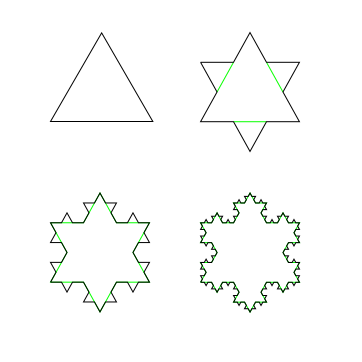
\includegraphics[width=0.3\textwidth]{KochFlake}
    \caption{The first four iterations of the Koch snowflake.}
    \label{fig:koch_snowflake}
\end{figure}

Then $K$ is homeomorphic to the circle $S^1$. For $s = \log/\log 3$, then we have $0 < \H^s(K) < \infty$ and in fact,
\begin{align*}
    \dim_{\H}(K) = \frac{\log 4}{\log 3}.
\end{align*}
\end{example}

\medskip

\begin{proposition}\label{prop_15}
In the definition of the Hausdorff measure, we can always assume that
\begin{enumerate}[label=(\alph*)]
    \item all sets $A_i$ are closed;
    
    \item or all sets $A_i$ are open.
\end{enumerate}
\end{proposition}
\begin{proof}
~\begin{enumerate}[label=(\alph*)]
    \item It is obvious, since $\diam \overline{A_i} = \diam A_i$ and we can replace $A_i$ by its closure.
    
    \item For any $E$ and fixed $\delta > 0$, there exists a family $\{A_i\}$ such that
    \begin{align*}
        \frac{\omega_s}{2^s} \sum^\infty_{i=1} (\diam A_i)^s \leq \H^s_{\varepsilon}(E) + \frac{\delta}{2}, \quad \diam A_i < \varepsilon.
    \end{align*}
    Let $U_i = \bigcup_{x \in A_i} B(x, r_i)$ such that $A_i \subset U_i$, and $U_i$ is open. Also, 
    \begin{align*}
        \diam U_i \leq \diam A_i + 2r_i < \varepsilon,
    \end{align*}
    for some $r_i$ small enough. And we can take $r_i$ small such that
    \begin{align*}
        \frac{\omega_s}{2^s} (\diam U_i)^s \leq \frac{\omega_s}{2^s} (\diam A_i)^s + \frac{\delta}{2^{i+1}}.
    \end{align*}
    
    Then, since $\{U_i\}$ is also a covering of $E$ with $\diam U_i < \varepsilon$, then
    \begin{align*}
        \H^s_{\varepsilon}(E) \leq \frac{\omega_s}{2^s} (\diam U_i)^s \leq \frac{\omega_s}{2^s} (\diam A_i)^s + \frac{\delta}{2} \leq \H^s_{\varepsilon}(E) + \delta,
    \end{align*}
    which implies
    \begin{align*}
        \H^s_{\varepsilon}(E) = \inf \frac{\omega_s}{2^s} (\diam U_i)^s,
    \end{align*}
    and the infimum is taken over all open coverings $\{U_i\}$.
\end{enumerate}
\end{proof}

\medskip

\begin{corollary}\label{coro_15}
In the definition of $\H^s$ on $\mathbb{R}$, we can take coverings by open intervals.
\end{corollary}
\begin{proof}
We can take coverings by open sets, but each open set is contained in an open interval of equal diameter.
\end{proof}

\medskip

Recall that $\H^s$ is a metric outer measure on a metric space $X$. Also, $\H^s$ restricted to $\BB(X)$ is countably additive, i.e. $\H^s$ is a Borel measure.\footnote{A {\em Borel measure} is any measure $\mu$  defined on the $\sigma$-algebra of Borel sets\cite{4}.}

\medskip

\begin{theorem}\label{theorem_119}
$\H^1$ is a measure on $\BB(\mathbb{R})$ such that
\begin{align}\label{theorem_119_1}
    \H^1((a,b)) = b - a,
\end{align}
if $- \infty < a < b < \infty$. Moreover, $\H^1$ is a unique measure with this property, that is, if $\mu$ is a measure on $\BB(\mathbb{R})$ such that $\mu((a,b)) = b - a$ if $- \infty < a < b < \infty$, then $\mu(E) = \H^1(E)$ for all $E \in \BB(\mathbb{R})$.
\end{theorem}

\medskip

$\H^1$ is a measure on $\BB(\mathbb{R})$. Assuming condition (\ref{theorem_119_1}), the uniqueness is easy to prove. 

\medskip

\begin{theorem}\label{theorem_120}
Let $X$ be a metric space, $\mu$ is a measure on $\BB(X)$, $X = \bigcup^\infty_{i=1}U_i$, where $U_i$ is open and $\mu(U_i) < \infty$. Suppose $\nu$ is another measure such that for any open set $U \subset X$, $\nu(U) = \mu(U)$, then for any $E \in \BB(X)$, $\nu(E) = \mu(E)$.
\end{theorem}
\begin{proof}
Since $X$ is a countable union of open sets with finite measure, by Theorem \ref{theorem_114}, then
\begin{align*}
    \mu(E) = \inf_{\substack{U \subset E\\ U - \text{open}}} \mu(U) = \inf_{\substack{U \subset E\\ U - \text{open}}} \nu(U) = \nu(E).
\end{align*}
\end{proof}

\medskip

Now let's use this theorem to prove the uniqueness of the previous theorem.

\medskip

\begin{proof}[Proof of Theorem \ref{theorem_119}]
~\begin{enumerate}[label=(\alph*)]
    \item Since $\H^1((a,b)) = \mu((a,b))$, by Corollary \ref{coro_15}, $\H^1(U) = \mu(U)$ for any open set $U \subset \mathbb{R}$. Thus, by Theorem \ref{theorem_120}, $\H^1(E) = \mu(E)$ for any $E \in \BB(\mathbb{R})$. Hence, the uniqueness is proved.
    
    \item It remains to prove that $\H^1((a,b)) = b - a$. 

    First, for any $\varepsilon > 0$, divide $[a,b]$ into small intervals $I_1, I_2, \cdots$, such that $\diam I_i < \varepsilon$. Note that $\sum^\infty_{i=1}\diam I_i = b - a$. Then,
    \begin{align*}
        \H^1_{\varepsilon}([a,b]) \leq \frac{\omega_1}{2^1} \sum^\infty_{i=1}(\diam I_i)^1 = b - a,
    \end{align*}
    since $\omega_1 = \operatorname{vol}\left(B^1(0,1)\right) = \operatorname{vol}\left((-1,1)\right) = 2$. Letting $\varepsilon \to 0$ gives $\H^1([a,b]) \leq b - a$.
    
    Second, taking infimum over coverings by open intervals $[a,b] \subset \bigcup^\infty_{i=1}U_i$, where $U_i$ is open interval and $\diam U_i < \varepsilon$ and then we have
    \begin{align*}
        \H^1_{\varepsilon}([a,b]) = \inf \sum^\infty_{i=1} \diam U_i.
    \end{align*}
    Since $[a,b]$ is compact, then there exists finite coverings of $[a,b]$ by open intervals. Choose a finite open covering $\{I_i\}$ from $\{U_i\}$ such that $[a,b] \subset \bigcup^k_{i=1} I_i$, then 
    \begin{align*}
        \sum^\infty_{i=1}\diam U_i \geq \sum^k_{i=1} \diamI_i \geq b - a.
    \end{align*}
    Taking infimum over all covering by open intervals with $\diamU_i < \varepsilon$ implies
    \begin{align*}
        \H^1([a,b]) = \inf \sum^\infty_{i=1} \diamU_i \geq b - a.
    \end{align*}
    
    It follows that $\H^1([a,b]) = b - a$, and thus $\H^1((a,b)) = b - a$.
\end{enumerate}
\end{proof}

\medskip

Let's talk more about properties of the Hausdorff measure.

\medskip

\begin{theorem}\label{theorem_121}
For $0 \leq s < \infty$ and every $E \subset X$ (not necessarily measurable), there is a sequence of open sets $V_1 \supset V_2 \supset V_3 \supset \cdots \supset E$ such that 
\begin{align*}
    E \subset \widetilde{E} \coloneqq \bigcap^\infty_{i=1} V_i,
\end{align*}
and $\H^s(E) = \H^s (\widetilde{E})$.
\end{theorem}
\begin{proof}
Note that $\widetilde{E}$ is $G_\delta$ set and hence Borel.

If $\H^s(E) = \infty$, take $v_i = X$ for all $I \in \mathbb{N}$ would yield the statement.

If $\H^s(E) < \infty$, by Proposition \ref{prop_15}, we can taking coverings by open sets in the definition of $\H^s$. So, we could find a covering $\{U_{i_j}\}$ such that
\begin{align*}
    E \subset \bigcup^\infty_{j=1} U_{i_j} \coloneqq U_i, \quad \diam U_{i_j} < \frac{1}{i}.
\end{align*}
and by the definition of $\H^s_{1/i} (E)$, we have
\begin{align*}
    \frac{\omega_s}{2^s} \sum^\infty_{j=1} \left(\diam U_{i_j}\right)^s \leq \H^s_{1/i} (E) + \frac{1}{i}.
\end{align*}

Let $V_i = \bigcap^i_{k=1}U_k$ be open, and clearly, $V_1 \supset V_2 \supset V_3 \supset \cdots \supset E$. Also, 
\begin{align*}
    \widetilde{E} \coloneqq \bigcap^\infty_{i=1} V_i = \bigcap^\infty_{i=1} U_i.
\end{align*}

We need to prove that $\H^s(E) = \H^s (\widetilde{E})$, and since $E \subset \widetilde{E}$ implies $\H^s(E) \leq \H^s(\widetilde{E})$, it remains to prove that $\H^s(E) \geq \H^s(\widetilde{E})$. Clearly,
\begin{align*}
    \widetilde{E} \subset U_i = \bigcup^\infty_{j=1} U_{i_j},
\end{align*}
then $\{U_{i_j}\}$ is a covering of $\widetilde{E}$ with $\diam U_{i_j} < 1/i$. Therefore,
\begin{align*}
    \H^s_{1/i}(\widetilde{E}) \leq \frac{\omega_s}{2^s} \sum^\infty_{j=1} \left(\diam U_{i_j}\right)^s \leq \H^s_{1/i}(E) + \frac{1}{i},
\end{align*}
and letting $i \to \infty$ gives
\begin{align*}
    \H^s(\widetilde{E}) \leq \H^s(E).
\end{align*}
Thus, $\H^s(E) = \H^s (\widetilde{E})$.
\end{proof}

\medskip

\begin{corollary}
If $0 \leq s < \infty$, $\H^s(X) < \infty$ and $E \subset X$ (not necessarily measurable), then \begin{align*}
    \H^s(E) =  \inf_{\substack{U \supset E\\ U - \text{open}}} \H^s(U).
\end{align*}
\end{corollary}
\begin{proof}
Let $V_i$ be as in the previous theorem. Clearly, $\H^1(V_1) \leq \H^s(X) < \infty$ and then, by Theorem \ref{theorem_16}(g) and Corollary \ref{coro_1111}, we have
\begin{align*}
    \lim_{i\to\infty} \H^1(V_i) = \H^s\left( \bigcap^\infty_{i=1} V_i\right) = \H^s(\widetilde{E}) = \H^s(E).
\end{align*}
\end{proof}

\medskip

\begin{remark}
Comparing this corollary with Theorem \ref{theorem_114}, we does not require $E$ being Borel set in the corollary.
\end{remark}

\medskip

\begin{theorem}
Let $E \subset X$ be any $\H^s$-measurable set, $0 \leq s < \infty$. If $\H^s(E) < \infty$, then \begin{align*}
    \H^s(E) = \sup_{\substack{C \subset E\\ C - \text{closed}}} \H^s(C).
\end{align*}
\end{theorem}
\begin{proof}
It is enough to prove that for any $\varepsilon > 0$, there exists a $F_\sigma$ subset of $E$ with $\H^s(F_\sigma) > \H^s(E) - \varepsilon$. For fixed $\varepsilon > 0$, by Theorem \ref{theorem_121}, let $\widetilde{E} = \bigcap^\infty_{i=1} V_i$, $V_i$ is open, such that $V_1 \supset V_2 \supset V_3 \supset \cdots \supset E$ and $\H^s(E) = \H^s(\widetilde{E})$. Hence, $\widetilde{E}$ is a $G_\delta$ set.

Since $E$ has finite measure, so does $\widetilde{E}$. Also, since $E \subset \widetilde{E}$, we have $\H^s(\widetilde{E} \setminus E) = 0$. 

We claim that each open set is a union of an increasing sequence of closed sets.\footnote{Let $E \subset X$ be open. Define $C_i = \left\{x \,|\, \operatorname{dist}(x, (X\setminus E)) \geq 1/i\right\}$, then $C_1 \subset C_2 \subset \cdots$, and $E = \bigcup^\infty_{i=1}C_i$. This is based on an example in $\mathbb{R}^n$ \cite{15}.}Then, $V_i$ is a union of such closed sets $F_i$. Since $E \subset V_i$, then there exists a closed set $F_i \subset V_i$ such that $\H^s(E \setminus F_i) < \varepsilon / 2^i$. Define
\begin{align*}
    F \coloneqq \bigcap^\infty_{i=1} F_i \subset \bigcap^\infty_{i=1} V_i = \widetilde{E},
\end{align*}
then
\begin{align*}
    \H^s(E \setminus F) = \H^s \left(\bigcup^\infty_{i=1} (E \setminus F_i)\right) < \varepsilon.
\end{align*}
Also, $\H^s(F \setminus E) \leq \H^s(\widetilde{E} \setminus E) = 0$. Therefore, there is a $G_\delta$ set of $G$ such that $F \setminus E \subset G$ and $\H^s(G) = 0$. 

Clearly, $F \setminus G$ is $F_\sigma$ set. Indeed, $G = \bigcap^\infty_{i=1} G_i$, and since $F \setminus G_i$ is closed, then
\begin{align*}
    F \setminus G = F \setminus \left(\bigcap^\infty_{i=1} G_i\right) = \bigcup^\infty_{i=1} (F \setminus G_i)
\end{align*}
is $F_\sigma$. Also, $F \setminus G \subset E$. Indeed, for $x \in F \setminus G$, we have $x \in F, x \notin G$. Since $F \setminus E \subset G$, then $x \in E$ and hence $F \setminus G \subset E$. Since $\H^s(G) = 0$, then 
\begin{align*}
    \H^s(F \setminus G) = \H^s(F) \geq \H^s(E \cap F) = \H^s(E) - \H^s(E \setminus F) > \H^s(E) - \varepsilon,
\end{align*}
and $F \setminus G$ is the subset we seek.
\end{proof}

\medskip

\begin{remark}
Comparing this theorem with Theorem \ref{theorem_114}, we does not require $X$ being of finite measure in this theorem.
\end{remark}

\medskip

\begin{theorem}
If $0 \leq s < \infty$ and $A_1 \subset A_2 \subset \cdots$ is an increasing sequence of not necessarily measurable sets, then
\begin{align*}
    \H^s \left(\bigcup^\infty_{i=1}A_i\right) = \lim_{i\to\infty} \H^s(A_i).
\end{align*}
\end{theorem}
\begin{proof}
It suffices to show $\H^s \left(\bigcup^\infty_{i=1}A_i\right) \geq \lim_{i\to\infty} \H^s(A_i)$, since the other direction is obvious by the fact that $\lim_{i\to\infty}A_i \subset \bigcup^\infty_{i=1}A_i$.

Let $A_i \subset \widehat{A}_i$, where $\widehat{A}_i$ is a Borel set\footnote{This is possible by Theorem \ref{theorem_121} that any set (not necessarily measurable) is contained in a $G_\delta$ set of equal measure.}and $\H^s(A_i) = \H^s(\widehat{A}_i)$. Define $\widetilde{A}_i = \bigcap^\infty_{j=i} \widehat{A}_j$, and $\widetilde{A}_i$ is also Borel. Then, $A_i \subset \widetilde{A}_i$. Indeed,
\begin{align*}
    A_i \subset A_{i+1} & \subset \widehat{A}_{i+1}, \\
    A_i \subset A_{i+2} & \subset \widehat{A}_{i+2}, \\
    \vdots & 
\end{align*}
and hence $A_i \subset \bigcap^\infty_{j=i} \widehat{A}_i = \widetilde{A}_i$. Also, since $A_i \subset \widetilde{A}_i \subset \widehat{A}_i$ and $\H^s(A_i) = \H^s(\widehat{A}_i)$, then $\H^s(A_i) = \H^s(\widetilde{A}_i)$. Note that $\widetilde{A}_1 \subset \widetilde{A}_2 \subset \cdots$ are measurable sets, thus we have 
\begin{align*}
    \H^s\left(\bigcup^\infty_{i=1}A_i\right) \leq \H^s\left(\bigcup^\infty_{i=1}\widetilde{A}_i\right) = \lim_{i\to\infty} \H^s(\widetilde{A}_i) = \lim_{i\to\infty} \H^s(A_i),
\end{align*}
which is exactly the inequality we need.
\end{proof}

\medskip

\section{Lebesgue measure}

Consider a closed interval in $\mathbb{R}^n$,
\begin{align}\label{closed_interval}
    P = [a_1,b_1] \times \cdots [a_n,b_n] \subset \mathbb{R}^n,
\end{align}
and we define its volume as 
\begin{align*}
    \left|P\right| \coloneqq (b_1-a_1) \cdots (b_n-a_n).
\end{align*}

\medskip

\begin{definition}
For any $A \subset \mathbb{R}^n$, the outer Lebesgue measure of $A$ is defined as
\begin{align*}
    \mathcal{L}^*_n(A) = \inf \sum^\infty_{i=1} \left|P_i\right|,
\end{align*}
where the infimum is taken over all coverings 
\begin{align*}
    A \subset \bigcup^\infty_{i=1} P_i,
\end{align*}
by intervals as in (\ref{closed_interval}). $\mathcal{L}^*_n$-measurable sets are called Lebesgue measurable. $\mathcal{L}^*_n$ restricted to Lebesgue measurable sets is called Lebesgue measure and is denoted by $\mathcal{L}_n$.
\end{definition}

\medskip

\begin{theorem}
$\mathcal{L}^*_n$ is a metric outer measure.
\end{theorem}

\medskip

\begin{remark}
By Theorem \ref{theorem_113}, $\BB(\mathbb{R}^n)$ is Lebesgue measurable.
\end{remark}

\medskip

\begin{corollary}\label{coro_17}
All Borel sets in $\mathbb{R}^n$ are Lebesgue measurable. 
\end{corollary}

\medskip

\begin{remark}\label{remark_17}
Recall that if $\mu^*$ is an outer measure, by Proposition \ref{prop_14}, all sets $A$ such that $\mu^*(A) = 0$ are $\mu^*$-measurable. Therefore, if $\mathcal{L}^*_n(A) = 0$, then $A$ is Lebesgue measurable, and $\mathcal{L}_n(A) = 0$. Note that $\mathcal{L}_n(A) = 0$ if and only if for all $\varepsilon > 0$, there is a family of closed intervals $\{P_i\}$ such that 
\begin{align*}
    A \subset \bigcup^\infty_{i=1} P_i, \quad \text{and} \quad \sum^\infty_{i=1} \left|P_i\right| < \varepsilon.
\end{align*}
\end{remark}

\medskip

\begin{theorem}\label{theorem_125}
If $P$ is a closed interval as in (\ref{closed_interval}), then $\mathcal{L}_n(P) = \left|P\right|$.
\end{theorem}

We often write $\left|A\right|$ to denote the Lebesgue measure of a Lebesgue measurable set $A$.

\begin{proof}
By definition,
\begin{align*}
    \mathcal{L}_n(P) = \inf \sum^\infty_{i=1} \left|P_i\right|, \quad P \subset \bigcup^\infty_{i=1} P_i.
\end{align*}
Taking covering of $P$ by itself, then $P \subset P$, then $\mathcal{L}_n(P) \leq \left|P\right|$.

It remains to show that $\left|P\right| \leq \sum^\infty_{i=1} \left|P_i\right|$. And we need a lemma to prove this.

\begin{lemma}\label{lemma_121}
If $P \subset \bigcup^k_{i=1} P_i$ is a finite covering of a closed interval $P$ by closed intervals $P_i$, then $\left|P\right| \leq \sum^k_{i=1} \left|P_i\right|$.
\end{lemma}
\begin{proof}[``Proof'']
We use the Riemann integral to prove this. Since $P \subset \bigcup^k_{i=1} P_i$, then
\begin{align*}
    \chi_P \leq \sum^k_{i=1} \chi_{P_i}.
\end{align*}
Then, we have
\begin{align*}
    \left|P\right| = \int_{\mathbb{R}^n} \chi_P \leq \sum^k_{i=1} \int_{\mathbb{R}^n} \chi_{P_i} = \sum^k_{i=1} \left|P_i\right|.
\end{align*}
\end{proof}
\begin{figure}[H]
    \centering
    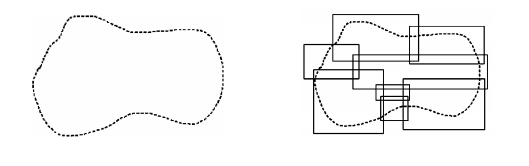
\includegraphics[width=0.6\textwidth]{closed_interval_covering.png}
    \caption{Example of a set covered by intervals(From \cite{6}).}
    \label{fig:closed_intervals}
\end{figure}

Now we can complete the proof of the theorem. Each interval $P_i$ is contained in a slightly bigger open interval $P_i^\varepsilon$ such that
\begin{align*}
    \left|\overline{P_i^\varepsilon}\right| = \left|P_i\right| + \frac{\varepsilon}{2^i},
\end{align*}
where $\overline{P_i^\varepsilon}$ is the closure of $P_i^\varepsilon$. Since $P$ is compact, then we can select a finite subcovering 
\begin{align*}
    P \subset \bigcup^k_{j=1} P_{i_j}^\varepsilon,
\end{align*}
and the lemma implies
\begin{align*}
    \left|P\right| \leq \sum^k_{j=1} \left|\overline{P_{i_j}^\varepsilon} \right| \leq \sum^\infty_{j=1} \left| \overline{P_{i}^\varepsilon} \right| = \sum^\infty_{i=1} \left|P_{i}\right| + \varepsilon,
\end{align*}
since $\varepsilon > 0$ is arbitraty, then the theorem follows.
\end{proof}

\medskip

\begin{proposition}
Let $P$ ba an open interval.
\begin{enumerate}
    \item[(a)] If $P = (a_1,b_1) \times \cdots (a_n,b_n)$ is a bounded interval, then 
    \begin{align*}
        \mathcal{L}_n(P) = (b_1-a_1) \cdots (b_n-a_n).
    \end{align*}
    
    \item[(b)] $\mathcal{L}_n(\partial P) = 0$.
    
    \item[(c)] If $P$ is an unbounded interval in $\mathbb{R}_n$ and has nonempty interior (i.e. each side has positive length and at least one of the sides has infinite length, which is of form $(-\infty,b), (a,\infty)$ or $(-\infty,\infty)$), then $\mathcal{L}_n(P) = \infty$.
\end{enumerate}
\end{proposition}
\begin{proof}
~\begin{enumerate}
    \item[(a)] For $P$, we could find a slightly smaller interval $P_\varepsilon$ contained in $P$ and a slightly bigger interval $P^\varepsilon$ which contains $P$, where\footnote{Here, $\bigtimes$ denotes the Cartesian product.}
    \begin{align*}
        P_\varepsilon = \bigtimes^n_{i=1} \left[a_i+\varepsilon,b_i-\varepsilon\right], \quad P^\varepsilon = \bigtimes^n_{i=1} \left[a_i-\varepsilon,b_i+\varepsilon\right].
    \end{align*}
    Then, $\mathcal{L}_n(P_\varepsilon) \leq \mathcal{L}_n(P) \leq \mathcal{L}_n(P^\varepsilon)$. Letting $\varepsilon \to 0$ yields the result:
    \begin{align*}
        (b_1-a_1) \cdots (b_n-a_n) \leftarrow \mathcal{L}_n(P_\varepsilon) \leq \mathcal{L}_n(P) \leq \mathcal{L}_n(P^\varepsilon) \to (b_1-a_1) \cdots (b_n-a_n).
    \end{align*}
    
    \item[(b)] $\mathcal{L}_n(\partial P) =  \mathcal{L}_n(\overline{P}) - \mathcal{L}_n(\operatorname{int}(P)) = 0$.
    
    \item[(c)] $P$ contains closed intervals of arbitrarily large measure.
\end{enumerate}
\end{proof}

\medskip

\begin{corollary}\label{coro_19161}
If $k < n$, then $\mathcal{L}_n (\mathbb{R}^k) = 0$.
\end{corollary}
\begin{proof}\footnote{This proof is based on that $\mathbb{R}^n\times\{0\}$ has measure zero in $\mathbb{R}^{n+1}$\cite{16}.} 
It suffice to show that $[-k,k]^{k} \times \{0\}^{n-k}$ has Lebesgue measure zero for all $k \in \mathbb{N}$.

For any $\varepsilon > 0$, choose $\delta > 0$ such that
\begin{align*}
    (2\delta)^{n-k} (2k+2\varepsilon)^k < \varepsilon.
\end{align*}
Now we define $$U_k = (-k-\varepsilon,k+\varepsilon)^k \times (-\delta,\delta)^{n-k},$$ 
and clearly $U_k$ contains $[-k,k]^{k} \times \{0\}^{n-k}$. Also, by the choice of $\delta$, $\mathcal{L}_n(U_k) < \varepsilon$, and since
\begin{align*}
    \mathcal{L}_n(\mathbb{R}^k) = \lim_{k\to\infty} \mathcal{L}_n\left([-k,k]^{k} \times \{0\}^{n-k}\right) < \varepsilon,
\end{align*}
we have $\mathcal{L}_n(\mathbb{R}^k) = 0$.
\end{proof}

\medskip

\begin{proof}[Second Proof of Corollary \ref{coro_19161}]
Finite intervals in $\mathbb{R}^k$ are contained in $\partial P$ for some interval $P$ in $\mathbb{R}^n$. Then, finite intervals in $\mathbb{R}^k$ have Lebesgue measure zero. Since $\mathbb{R}^k$ is a union of finite intervals in $\mathbb{R}^k$, then $\mathcal{L}_n(\mathbb{R}_k) = 0$.
\end{proof}

\medskip

\begin{theorem}[{\bf Steinhaus}]
Prove that is a set $E \subset \mathbb{R}$ has positive measure $\mathcal{L}_1(E) > 0$, then the set $E -E = \{x - y \,:\, x,y\in E\}$ contains an interval.
\end{theorem}
\begin{proof}
The following is a simple proof by Karl Stromberg \cite{30}. For any $\varepsilon > 0$, there exist a closed set $F$ and an open set $G$ such that $F \subset E \subset G$ and
\begin{align*}
    \mu(G) - \varepsilon < \mu(E) < \mu(F) + \varepsilon,
\end{align*}
where $\mu$ is the Lebesgue measure. Also, without loss of generality, we could assume $2 \mu(F) > \mu(G)$. Since $F \subset G$, for each $x \in F$, there is a neighborhood $W_x$ of $0$ such that $x + W_x \subset G$. Furthermore, there is a neighborhood $V_x$ of $0$ such that $2V_k \subset W_x$, i.e. if $W_x = (-\varepsilon,\varepsilon)$, then we can take $V_x = (-\varepsilon/2,\varepsilon/2)$.

Now, the family $\{x_i + V_{x_i} \,:\, x_i\in F \}$ is an open covering of $F$. Since $F$ is closed, it is compact, and hence there is a finite subcovering $\{x_i + V_{x_i}\}^n_{i=1}$. Let $V \coloneqq \bigcap^n_{i=1} V_{x_i}$, then
\begin{align*}
    F + V \subset \bigcup^n_{i=1} \left(x_i + V_{x_i}\right) + V \subset \bigcup^n_{i=1} \left(x_i + 2V_{x_i}\right) \subset G.
\end{align*}
Let $v \in V$ and suppose $(F + v) \cap F = \emptyset$, then $2 \mu(F) = \mu(F + v) + \mu(F) < \mu(G)$, which is a contradiction. Hence, for all $v \in V$, there exist $x_1, x_2 \in F \subset E$ such that $v + x_1 = x_2$, which means $E - E$ contains a neighborhood of $0$.
\end{proof}

\medskip

\begin{theorem}\label{theorem_122}
For an arbitrary set $E \subset \mathbb{R}^n$ (not necessarily measurable),
\begin{align*}
    \mathcal{L}_n^*(E) = \inf_{\substack{U \subset E\\ U - \text{open}}} \mathcal{L}_n(U).
\end{align*}
\end{theorem}
\begin{proof}
Clearly, $\mathcal{L}_n^*(E) \leq \inf_{U \subset E} \mathcal{L}_n(U)$. It remains to show the other direction.

By definition, $\mathcal{L}^*_n(E) = \inf \sum^\infty_{i=1} \left|P_i\right|$, $E \subset \bigcup_i P_i$, where $P_i$ are closed intervals. Now let $P_i^\varepsilon$ be open interval such that $P_i \subset P_i^\varepsilon$ and
\begin{align*}
    \left|P_i^\varepsilon\right| = \left|P_i\right| + \frac{\varepsilon}{2^i}.
\end{align*}

This approximation yields
\begin{align*}
    \mathcal{L}_n^*(E) = \inf \sum^\infty_{i=1} \left|P_i\right|, \quad E \subset \bigcup^\infty_{i=1} P_i,
\end{align*}
where $P_i$ are open. Indeed, by the subadditivity of the outer measure, $\mathcal{L}_n^*(E) \leq \sum^\infty_{i=1} \left|P_i\right|$, which implies $\mathcal{L}_n^*(E) \leq \inf \sum^\infty_{i=1} \left|P_i\right|$. Also, every closed interval can be approximated by a slighter bigger open interval, and this implies the equality.

Now, for $E \subset \bigcup^\infty_{i=1}P_i$, $P_i$ are open intervals, by Theorem \ref{theorem_125},
\begin{align*}
    \sum^\infty_{i=1} \left|P_i\right| \geq \left|\bigcup^\infty_{i=1}P_i\right| = \mathcal{L}_n\left(\bigcup^\infty_{i=1}P_i\right) \geq \inf_{U \supset E} \mathcal{L}_n(U),
\end{align*}
where $U$ is open, and taking the infimum over all coverings $E \subset \bigcup^\infty_{i=1}P_i$ by open intervals yields
\begin{align*}
    \mathcal{L}_n^*(E) \geq  \inf_{U \supset E} \mathcal{L}_n(U).
\end{align*}
\end{proof}

\medskip

So how to compute $\mathcal{L}_n(U)$ for open set $U$? Let's introduce the dyadic cubes. Consider cubes vertices in $\mathbb{Z}^n$, and divide each cubes into $2^k$ cubes, $k = 0,1,2,\cdots$. 

\medskip

\begin{theorem}\label{theorem_123}
An arbitrary open set in $\mathbb{R}^n$ is a union of closed dyadic cubes with pairwise disjoint interiors. Then the Lebesgue measure of the open set equals the sum of the measures of these cubes.
\end{theorem}
\begin{figure}[H]
    \centering
    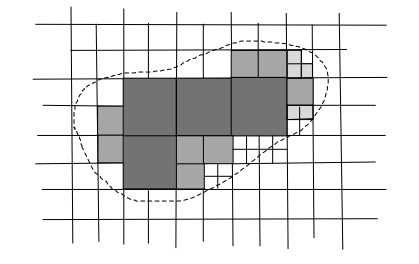
\includegraphics[width=0.5\textwidth]{dyadic_cube.png}
    \caption{Example of open set represented by the dyadic cubes in $\mathbb{R}^2$(From \cite{6}).}
    \label{fig:dyadic_cube}
\end{figure}

\medskip

Recall that by a $G_\delta$ set we mean a set of the form $G = \bigcap^\infty_{i=1} G_i$, where $G_i \subset X$ are open and by a $F_\sigma$ set we mean a set of the form $F = \bigcap^\infty_{i=1} F_i$, where $F_i \subset X$ are closed. Clearly, all $G_\delta$ and $F_\sigma$ sets are Borel sets.

\medskip

\begin{theorem}\label{theorem_124}
Let $A \subset \mathbb{R}^n$, then the following conditions are equivalent:
\begin{enumerate}[label=(\alph*)]
    \item $A$ is Lebesgue measurable;
    
    \item For every $\varepsilon > 0$, there is an open set $G$ such that $A \subset G$ and $\L^*_n(G\setminus A) < \varepsilon$;
    
    \item There is a $G_\delta$ set $H$ such that $A \subset H$ and $\L^*_n(H\setminus A) = 0$;
    
    \item For every $\varepsilon > 0$, there is a closed set $F$ such that $F \subset A$ and $\L^*_n(A\setminus F) < \varepsilon$;
    
    \item There is a $F_\sigma$ set $M$ such that $M \subset A$ and $\L^*_n(A\setminus M) = 0$;
    
    \item For every $\varepsilon > 0$, there is an open set $G$ and a closed set $F$ such that $F \subset A \subset G$ and $\L_n(G \setminus F) < \varepsilon$.
\end{enumerate}
\end{theorem}
\begin{proof}
~\begin{enumerate}
    \item[(a)]$\Rightarrow$ (b) Every measurable set can be represented as a union of sets with finite measure $A = \bigcup^\infty_{i=1}A_i$, $\L_n(A_i) < \infty$, where $A_i$ is Lebesgue measurable and $\L_n(A_i) < \infty$. Indeed, since $A$ is arbitrary Lebesgue measurable set, then we can define $A_i = A \cap B(0,i), i = 1,2,\cdots,n$, where $B(0,i) \subset \mathbb{R}^n$ is the closed ball centered at the origin with radius $i$. Since $A$ is measurable and bounded, then $\L_n(A_i) < \infty$. By Theorem \ref{theorem_122}, for every $i$, there is an open set $G_i$ such that $A_i \subset G_i$ and $\L_n(G_i\setminus A_i) < \varepsilon / 2^i$. Hence $A \subset \bigcup^\infty_{i=1} G_i \coloneqq G$, and $\L_n(G \setminus A) \leq \sum^\infty_{i=1} \L_n(G_i \setminus A_i) = \varepsilon$.\footnote{Indeed, since $(G \setminus A) \subset (G \setminus A_i)$, then $G \setminus A = \bigcup^\infty_{i=1} (G_i \setminus A) \subset \bigcup^\infty_{i=1} (G_i \setminus A_i).$}
    
    \item[(b)]$\Rightarrow$ (c) By (b), we can find an open set $G_i$ such that $A \subset G_i$ and $\L_n^*(G_i\setminus A) < 1/i$. Let $H = \bigcap^\infty_{i=1} G_i$, then $H$ is $G_\delta$ set and $A \subset H$. Then, $\L_n^*(H\setminus A) \leq 1/i$ for every $i \in \mathbb{N}$, which yields $\L_n^*(H\setminus A) = 0$. Hence, by Remark \ref{remark_17}, $\L_n(H \setminus A) = 0$.
    
    \item[(c)]$\Rightarrow$ (a) We know that $A = H \setminus (H \setminus A)$, $H$ is $G_\delta$ set and it follows from Corollary \ref{coro_17}, $H$ is measurable. Since $H \setminus A$ is measurable, hence $A$ is also measurable.
    
    \item[(a)] $\Leftrightarrow	$ (d) $\Leftrightarrow$ (e)\footnote{It follows from the equivalence of the conditions (a), (b) and (c) applied to the set $\mathbb{R}^n\setminus A$.} $A$ is measurable, then $\mathbb{R}^n \setminus A$ is also measurable. By (b), there is an open set $G$ such that $(\mathbb{R}^n \setminus A) \subset G$ and $\L_n^*(G \setminus (\mathbb{R}^n \setminus A)) < \varepsilon$. Let $F \coloneqq \mathbb{R}^n \setminus G \subset A$, then $F$ is closed. Since $A \setminus F = G \setminus (\mathbb{R}^n \setminus A)$, then $\L_n(A \setminus F) < \varepsilon$, which indicates (d).
    
    Now for $\mathbb{R}^n \setminus A$, by (c), there exists a $G_\delta$ set $H$ such that $(\mathbb{R}^n \setminus A) \subset H$ and $\L_n^*(H \setminus (\mathbb{R}^n \setminus A)) = 0$. Let $M \coloneqq \mathbb{R}^n \setminus H \subset A$, then $M$ is a $F_\sigma$ set. Since $A \setminus M = H \setminus (\mathbb{R}^n \setminus A$, then $\L_n(A \setminus M) = 0$, which indicates (e).
    
    \item[(a)] $\Rightarrow$ (f) By (d), there is a closed set $F \subset A$ such that $\L_n(A \setminus F) < \varepsilon/2$. By (b), there is an open set $G \supset A$ such that  $\L_n(G \setminus A) < \varepsilon/2$. Hence, $F \subset A \subset G$ and $\L_n(G \setminus F) < \varepsilon/2 + \varepsilon/2 = \varepsilon$.
    
    \item[(f)] $\Rightarrow$ (a) There exists a closed set $F_i$ and an open set $G_i$ such that $\L_n(G_i\setminus F_i) < 1/i$. Let $H \coloneqq \bigcap^\infty_{i=1} G_i$, then $H$ is a $G_\delta$ set and $A \subset H$. Then,
    \begin{align*}
        \L_n^*(H \setminus A) \leq \L_n^*\left(H \setminus \bigcup^\infty_{i=1}F_i\right) \leq \L_n^*\left(\bigcap^\infty_{i=1}(G_i \setminus F_i)\right) = 0.
    \end{align*}
    Therefore, (f) implies (c), and hence (a).\footnote{The second inequality follows from that if $x \in H \setminus \bigcup^\infty_{i=1}F_i$, then $x \in G_i$ but $x \notin F_i$ for all $i$. Hence, $x \notin G_i \setminus F_i$ for all $i$, which is equivalent to $x \in \bigcap^\infty_{i=1} (G_i \setminus F_i)$.}
\end{enumerate}
\end{proof}

\medskip

The Lebesgue measure has an important property of being invariant under translations, i.e. $E \subset \mathbb{R}^n$ is Lebesgue measurable if and only if for all $a \in \mathbb{R}^n$, $E+a = \{x+a\,|\, x \in E\}$ is Lebesgue measurable. Moreover, $\L_n(E) = \L_n(A)$. Now we want to discuss an example of set that is not Lebesgue measurable.

\medskip

\begin{theorem}[\bf Vitali]\label{Vitali_theorem}
There is a set $E \in \mathbb{R}^n$ which is not Lebesgue measurable.
\end{theorem}
\begin{proof}[``Idea'']
We will prove the theorem for $n = 1$, and the same argument can be applied to an arbitrary $n$. The idea is to find a countable family of pairwise disjoint and isometric sets $V_i$ whose union $E$ contains $(0,1)$ and is contained in $(-1,2)$, that is find countable many $V_i \in (-1,2)$ such that $V_i \cap V_j = \emptyset$ for all $i \neq j$, and for all $i$, there is a set $V \in (0,1)$ such that $V_i$ is a translation of $V$. Also, $(0,1) \subset \bigcup^\infty_{i=1} V_i \subset (-1,2)$. Then $V$ cannot be Lebesgue measurable.

Suppose $V$ is Lebesgue measurable. Since $V_i$ is a translation of $V$, then $\L_1(V) = \L_1(V_i)$ for all $i$. If $\L_1(V) = 0$, then
\begin{align*}
    \L_1((0,1)) \leq \sum^\infty_{i=1} \L_1(V_i) = 0,
\end{align*}
which is a contradiction.

If $\L_1(V) > 0$, then
\begin{align*}
    3 = \L_1((-1,2)) \geq \L_1\left(\bigcup^\infty_{i=1} V_i\right) = \sum^\infty_{i=1} \L_1(V_i) = \infty,
\end{align*}
which is also a contradiction. Thus, $V$ is not Lebesgue measurable.
\end{proof}

\medskip

Now let's construct such $V$ properly.

\medskip

\begin{proof}[Proof of Vitali Theorem]
Consider the following equivalence relation among point in $(0,1)$, $x \sim y$ if $x - y \in \mathbb{Q}$. Therefore, $(0,1)$ is the union of a family $\mathcal{F}$ of pairwise disjoint equivalent classes 
\begin{align*}
    \{x\} = \{y \in (0,1)\,:\, x - y \in \mathbb{Q}\}.
\end{align*}
Then $\{x\} = \{y\}$ if and only if $x \sim y$. Also, $\mathbb{F} = \{\{x\}\,|\, x \in (0,1)\}$, then 
\begin{align*}
    (0,1) = \bigcup_{\{x\} \in \mathcal{F}} \{x\}.
\end{align*}
By the axiom of choice,\footnote{The construction of $V$ involves the axiom of choice, see Theorem \ref{axiom_of_choice}.}there is a set $V \subset (0,1)$ such that $V$ contains exactly one element from each equivalence class. Then, $V$ has following properties:
\begin{enumerate}[label=(\alph*)]
    \item If $x,y \in V, x \neq y$, then $x - y \notin \mathbb{Q}$. Otherwise, $\{x\} = \{y\}$.
    
    \item If $x \in (0,1)$, then there is $a \in \mathbb{Q}$ such that $x - a \in V$. Indeed, there is $y \in \{x\}$ such that $y \in V$, then $x \sim y$, which implies $y = x - a$, $a \in \mathbb{Q}$.\label{vitali_property_b}
\end{enumerate}

Next we will prove that $V$ is not Lebesgue measurable. Let
\begin{align*}
    E = \bigcup_{a\in\mathbb{Q}\cap(-1,1)} V_a,
\end{align*}
where $V_a = V + a = \{x+a\,:\, x\in V\}$. Clearly,
\begin{enumerate}[label=(\roman*)]
    \item $V_a \cap V_b = \emptyset$, if $a,b \in \mathbb{Q}, a \neq b$. Indeed, suppose $x \in (V_a \cap V_b)$, then $x = x_1 + a$ and $x = x_2 + b$, then $x_1 - x_2 = b - a \in \mathbb{Q}$. Therefore, $\{x_1\} = \{x_2\}, x_1 \neq x_2$. Hence, $x_1, x_2 \in V$ are two different points from the same equivalence class, which is a contradiction.
    
    \item $(0,1) \subset E \subset (-1,2)$. Clearly, $V \subset (0,1)$, $a \in (-1,1)$, then $V_a \subset (-1,2)$ for all $a \in \mathbb{Q}\cap(-1,1)$. Therefore, $E \subset (-1,2)$. Now let $x \in (0,1)$, then there is $y \in \mathbb{Q}$ such that $x - y \in V \subset (0,1)$ by property \ref{vitali_property_b} above. And since $x - y \in (0,1)$, then $y \in \mathbb{Q} \cap (-1,1)$, which implies $x \in V_y \subset E$. Hence, $(0,1) \subset E$.
\end{enumerate}
Now suppose $V$ is Lebesgue measurable, then each $V_a$ is measurable and since $V_a$ is a translation of $V$, then $\L_1(V) = \L_1(V_a)$. If $\L_1(V) > 0$, then $\L_1(E) = \infty$, which is a contradiction. If $\L_1(V) = 0$, then $\L_1(E) = 0$, which is also a contradiction. Thus, $V$ is not Lebesgue measurable.
\end{proof}

\medskip

The Lebesgue measure is translation invariant and $\L_n([0,1]^n) = 1$, and this two properties uniquely determine Lebesgue measure. This indicates that the
Lebesgue measure is in a sense the only natural way of measuring length, area, volume of general sets in finite-dimensional Euclidean spaces, which gives the following theorem.

\medskip

\begin{theorem}\label{theorem_126}
If $\mu$ is a measure on $\BB(\mathbb{R}^n)$ such that $\mu(a+E) = \mu(E)$ for all $a \in \mathbb{R}^n$ and $E \subset \BB(\mathbb{R}^n)$ and $\mu([0,1]^n) = 1$, then $\mu(E) = \L_n(E)$ on $\BB(\mathbb{R}^n)$.
\end{theorem}
\begin{proof}
By Corollary \ref{coro_191}, it suffice to prove that $\mu(U) = \L_n(U)$ for all open set $U$. 

Let $K$ be a face of the boundary $\partial Q$ of a unit cube $Q = [0,1]^n$, and there are $2^n$ faces. There are infinitely many pairwise parallel copies of $K$ inside $Q$, denoted by $K_1, K_2, \cdots$, shown in the following
\begin{figure}[H]
    \centering
    \begin{tikzpicture}[scale=2.5]
        \draw[-] (0,0)--(1,0)node[pos=.5,below]{$Q$};
        \draw[-] (1,0)--(1,1);
        \draw[-] (1,1)--(0,1);
        \draw[-] (0,1)--(0,0);
        \draw[-] (0,1)--(0.424,1.424);
        \draw[-] (0.424,1.424)--(1.424,1.424);
        \draw[-] (1.424,0.424)--(1.424,1.424);
        \draw[dotted,-] (0,0)--(0.424,0.424);
        \draw[dotted,-] (0.424,0.424)--(1.424,0.424);
        \draw[dotted,-] (0.424,0.424)--(0.424,1.424);
        \draw[fill=gray] (1,0)--(1,1)--(1.424,1.424)--(1.424,0.424);
        \filldraw[black] (1.106,0.7) circle (0pt) node[anchor=west]{$K$};
        \draw[-] (1,0)--(1.424,0.424);
        \draw[-] (1,1)--(1.424,1.424);
        
        \draw[-] (0.5,0)--(0.5,1);
        \draw[-] (0.5,1)--(0.912,1.424);
        \draw[dotted,-] (0.912,1.424)--(0.912,0.424);
        \draw[dotted,-] (0.912,0.424)--(0.5,0);
        \filldraw[black] (0.606,0.7) circle (0pt) node[anchor=west]{$K_1$};
    \end{tikzpicture}
    \caption{Parallel copy $K_1$ of face $K$ inside a $3$-dimensional unit cube.}
    \label{fig:unit_cube_cut}
\end{figure}
Since $\mu$ is translation invariant, then 
\begin{align*}
    \mu(K_1) = \mu(K_2) = \cdots = \mu(K).
\end{align*}
Since $\mu(Q) = 1$, then $\mu(K) = 0$. Indeed, otherwise $\mu(K) > 0$, then $1 = \mu(Q) \geq \mu\left(\bigcup_i K_i\right) = \sum_i \mu(K_i) = \infty$, which is a contradiction. This implies that $\mu(\partial Q) = 0$. 

Let $k \in \mathbb{N}$, $k > 0$ and let $Q_k = (0,2^{-k})^n$, then $\mu(\partial Q_k) = 0$. Note there are $2^{kn}$ open cubes contained in $Q$, denoted by $A_1, A_2, \cdots, A_{2^{kn}}$,\footnote{These are the dyadic cubes.}each being a translation of $Q_k$. Then, 
\begin{align*}
    2^{kn} \mu(Q_k) = \sum^{2^{kn}}_{i=1} \mu(A_i) \leq \mu(Q) = 1,
\end{align*}
which implies $\mu(Q_k) \leq 2^{-kn}$. Since $\mu(\partial Q_k) = 0$, then 
\begin{align*}
    \mu(\overline{Q}_k) = \mu(Q_k) \leq 2^{-kn}.
\end{align*}

On the other hand, $Q$ can be covered by $2^{kn}$ cubes $\overline{A}_1, \overline{A}_2, \cdots, \overline{A}_{2^{kn}}$, then
\begin{align*}
    1 = \mu(Q) \leq \sum^{2^{kn}}_{i=1} \mu(\overline{A}_i) = 2^{kn} \mu(\overline{Q}_k).
\end{align*}
Hence, $\mu(\overline{Q}_k) = \mu(Q_k) = 2^{-kn}$. Also, since $\L_n(\overline{Q}_k) = 2^{-kn}$, we have $\mu(\overline{Q}_k) = \L_n(\overline{Q}_k)$. Therefore, $\L_n = \mu$ on the dyadic cubes. 

For any open set $U \subset \mathbb{R}^n$, by Theorem \ref{theorem_123}, then $U$ can be written as a union of the dyadic cubes, that is 
\begin{align*}
    U = \bigcup^\infty_{i=1} \overline{D}_i = \left(\bigcup^\infty_{i=1} D_i\right) \cup \left(\bigcup^\infty_{i=1} \partial D_i\right),
\end{align*}
and since $\L_n(\bigcup_i \partial D_i) = \mu(\bigcup_i \partial D_i) = 0$, then 
\begin{align*}
    \mu(U) = \mu\left(\bigcup^\infty_{i=1} D_i\right) = \sum^\infty_{i=1} \mu(D_i) = \sum^\infty_{i=1} \L_n(D_i) = \L_n\left(\bigcup^\infty_{i=1} D_i\right) = \L_n(U),
\end{align*}
and thus the theorem follows.
\end{proof}

\medskip

Observe that by Corollary \ref{coro_1111}, $\H^n$ is a measure on $\BB(\mathbb{R}^n)$, and $\H^n(a+E) = \H^n(E)$ and $\H^n([0,1]^n) < \infty$. If we can prove $\H^n([0,1]^n) = 1$, then $\H^n = \L_n$ on $\BB(\mathbb{R}^n)$.

\medskip

\begin{theorem}
$\H^n = \L_n$ on $\BB(\mathbb{R}^n)$.
\end{theorem}
\begin{proof}
This theorem follows from the next theorem.
\end{proof}

\medskip

\begin{theorem}\label{theorem_129}
For any $A \subset \mathbb{R}^n$, $0 < \delta \leq \infty$, we have
\begin{align*}
    \L_n^*(A) = \H^n(A) = \H^n_{\delta} (A).
\end{align*}
\end{theorem}

\medskip

Before proving this theorem, we need some propositions and theorems. Recall that $E \subset \mathbb{R}^n$ has measure zero if and only if for any $\varepsilon > 0$, there is a covering $E \subset \bigcup_i P_i$ such that $\sum_i \left|P_i\right| < \varepsilon$.

\medskip

\begin{proposition}\label{prop_18}
$E \subset \mathbb{R}^n$ has measure zero if and only if for any $\varepsilon > 0$, there is a family of balls $\{B(x_i,r_i)\}^\infty_{i=1}$ such that
\begin{align*}
    E \subset \bigcup^\infty_{i=1} B(x_i,r_i), \quad \sum^\infty_{i=1} r_i^n < \varepsilon.
\end{align*}
\end{proposition}
\begin{proof}
~\begin{enumerate}
    \item[($\Leftarrow$)] Each ball $B(x_i,r_i)$ is contained in a cube $Q_i$ of sidelength $2r_i$ so we can cover $E$ by cubes $E \subset \bigcup_i Q_i$ such that
    \begin{align*}
        \sum^\infty_{i=1} \left|Q_i\right| = \sum^\infty_{i=1} (2r_i)^n < 2^n \varepsilon,
    \end{align*}
    letting $\varepsilon \to 0$ proves this direction.
    
    \item[($\Rightarrow$)] Since $\L_n(E) = 0$, then there is an open set $U$ such that $E \subset U$, $\L_n(U) < 2^{-n}n^{-n/2} \varepsilon$. Also, by Theorem \ref{theorem_123}, $U$ is a union of the closed dyadic cubes $\overline{D}_i$ with disjoint interiors $D_i$, that is $U = \bigcup^\infty_{i=1} \overline{D}_i$. Any cube $\overline{D}$ of sidelength $\ell$ is contained in a ball of radius $r = 2\sqrt{n}\ell$\cite{17}, and $r^n = 2^nn^{n/2}|\overline{D}|$. 
    
    Therefore, $\overline{D}_i \subset B(x_i,r_i)$ of radius $r_i$ similar to the above. Thus, $U \subset \bigcup^\infty_{i=1} B(x_i,r_i)$, and
    \begin{align*}
        \sum^\infty_{i=1} r_i^n = 2^nn^{n/2} \sum^\infty_{i=1} |\overline{D}|\, = 2^nn^{n/2} \L_n(U) < \varepsilon.
    \end{align*}
\end{enumerate}
\end{proof}

\medskip

\begin{theorem}[{\bf Brunn–Minkowski inequality}]\label{theorem_130}
Let $n \geq 1$ and let $\mu$ denote the Lebesgue measure on $\mathbb{R}^n$. Let $A$ and $B$ be two nonempty compact subsets of $\mathbb{R}^n$. Then,
\begin{align*}
    \mu(A + B)^{1/n} \geq \mu(A)^{1/n} + \mu(B)^{1/n}.
\end{align*}
\end{theorem}

\medskip

See some applications of Brunn–Minkowski inequality and the proof of this inequality in Appendix \ref{appendix_d}.

\medskip

\begin{definition}
We say a set $W \subset \mathbb{R}^n$ is convex if for any $x,y \in W$ and $t \in [0,1]$, $tx + (1-t)y \in W$.
\end{definition}

\medskip

\begin{definition}
If $E \subset \mathbb{R}^n$ is compact, then its closed convex hull $\mathcal{C}(E)$ of $E$ is defined as the intersection of all convex closed sets that contain $E$.
\end{definition}

\begin{figure}[H]
    \centering
    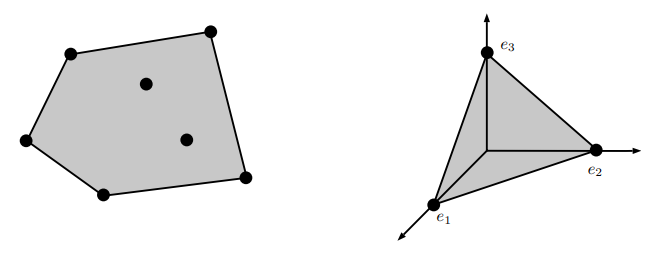
\includegraphics[width=0.6\textwidth]{convex_hull.png}
    \caption{The convex hull of several points in the plane and the convex hull of the standard basis in $\mathbb{R}^3$ (From \cite{31}).}
    \label{fig:convex_hull}
\end{figure}

\medskip

Clearly, $\mathcal{C}(E)$ is convex, compact and is the smallest convex set that contains $E$. Also, $\diam E = \diam (\mathcal{C}(E))$.

\medskip

\begin{theorem}[{\bf Isodiametric inequality}]\label{theorem_131}
If $E \subset \mathbb{R}^n$ is compact, then
\begin{align*}
    \mu(E) \leq \mu(\mathcal{C}(E)) \leq \frac{\omega_n}{2^n} (\diam E)^n,
\end{align*}
where $\omega_n$ is the volume of the unit ball in $\mathbb{R}^n$, see Theorem \ref{theorem_B4}.
\end{theorem}
\begin{proof}
It suffices to assume tat $E$ is convex. Indeed, if we know the result for convex sets, then for any $E \subset \mathbb{R}^n$, since $\diam E = \diam (\mathcal{C}(E))$, we have
\begin{align*}
    \mu(E) \leq \mu(\mathcal{C}(E)) \leq \frac{\omega_n}{2^n} (\diam (\mathcal{C}(E)))^n = \frac{\omega_n}{2^n} (\diam E)^n.
\end{align*}

Now we claim that it suffices to show that there is a set $F$ that is convex, compact and central symmetric with respect to $0$ (i.e., if $x \in F$, then $-x \in F$) such that 
\begin{align*}
    \mu(F) \geq \mu(E), \quad \diam F \leq \diam E.
\end{align*}
Indeed, first we have
\begin{align}\label{theorem_131_equ1}
    F \subset \overline{B}\left(0, \frac{\diam F}{2}\right).
\end{align}
To see this, note that there two points $x,y \in F$ such that $d(x,y) = \diam F$, and by the triangle inequality, one of the following is satisfied
\begin{align*}
    d(x,0) \geq \frac{d(x,y)}{2} \,\,\text{or}\,\, d(y,0) \geq \frac{d(x,y)}{2}.
\end{align*}
Suppose we have the former one: $d(x,0) \geq d(x,y)/2$, since $-x \in F$, we have $d(x,-x) = 2d(x,0) \geq d(x,y) = \diam F$, which implies that only equality can hold here. Hence, \eqref{theorem_131_equ1} holds.

It remains to prove the existence of such $F$ in the claim. Let $E' = \{-x \,:\, X \in E\}$, and define
\begin{align*}
    F = \frac{E + E'}{2} = \left\{\frac{x - y}{2} \,:\, x, y \in E\right\}.
\end{align*}
Then, we have
\begin{enumerate}[label=(\alph*)]
    \item Clearly, $F$ is central symmetric and $F$ is convex, since for $(x-y)/2, (x'-y')/2 \in F$,
    \begin{align*}
        t \frac{x - y}{2} + (1 - t) \frac{x' - y'}{2} = \frac{tx - (1-t)x' - (ty + (1-t)y')}{2} \in F.
    \end{align*}
    
    By Brunn–Minkowski theorem \ref{theorem_130}, and the fact that $\mu(aE) = a^n \mu(E)$, we have
    \begin{align*}
        \mu(F)^{1/n} = \mu\left(\frac{E+E'}{2}\right)^{1/n} \geq \mu\left(\frac{E}{2}\right)^{1/n} + \mu\left(\frac{E'}{2}\right)^{1/n} = \frac{\mu(E)^{1/n}}{2} + \frac{\mu(E')^{1/n}}{2} = \mu(E)^{1/n},
    \end{align*}
    which implies $\mu(F) \geq \mu(E)$.
    
    \item Let $x,y \in F$ such that $d(x,y) = \diam F$. Also, by definition of $F$, $x = (x' - x'')/2, y = (y' - y'')/2$ for some $x',x'',y',y'' \in E$. Then,
    \begin{align*}
        \diam F = d(x - y) = \frac{1}{2} d(x'-x'',y'-y'') \leq \frac{1}{2} d(x',y') + \frac{1}{2} d(x'',y'') \leq \diam E,
    \end{align*}
    which implies $\diam F \leq \diam E$.
\end{enumerate}

Now $F$ exists and by the claim, we have
\begin{align*}
    \mu(E) \leq \mu(F) \leq \omega_n \left(\frac{\diam F}{2}\right)^n \leq \frac{\omega_n}{2^n} (\diam E)^2,
\end{align*}
which proves the theorem.
\end{proof}

\medskip

\begin{lemma}\label{lemma_12}
If $Z \subset \mathbb{R}^n$ and $\L_n(Z) = 0$, then $\H^n_{\delta}(Z) = 0$ for any $0 < \delta \leq \infty$.
\end{lemma}
\begin{proof}
Since $\L_n(Z) = 0$, then for any $\varepsilon > 0$, there is a covering $Z \subset \bigcup^\infty_{i=1} B(x_i,r_i)$ of open balls with $\sum^\infty_{i=1} r_i^n < \varepsilon$. For any $0 < \varepsilon < (\delta/2)^n$, we have
\begin{align*}
    \frac{\omega_n}{2^n} \sum^\infty_{i=1}(\diam B_i)^n = \omega_n \sum^\infty_{i=1} r_i^n < \omega_n \varepsilon = \omega_n \left(\frac{\delta}{2}\right)^n,
\end{align*}
which implies $\diam B_i < \delta$, and hence $\H^n_{\delta}(Z) < \omega_n \varepsilon$. Letting $\varepsilon \to 0$ yields the lemma.
\end{proof}

\begin{lemma}\label{lemma_13}
If $U \subset \mathbb{R}^n$ is open and bounded, then for any $\delta > 0$, there is a family of pairwise disjoint closed balls $\overline{B}_i \subset U$ with $\diam B_i < \delta$ and such that
\begin{align*}
    \left|U \setminus \bigcup^\infty_{i=1} \overline{B}_i\right| = 0.
\end{align*}
\end{lemma}
\begin{proof}
Let $Q \subset \mathbb{R}^n$ be a cube and $\overline{B} \subset \operatorname{int} Q$ be a ball. Then $\left|Q \setminus \overline{B}\right| = \theta \left|Q\right|$ for some $0 < \theta < 1$. 

Now let $U_1 = U$ and $U = \bigcup^\infty_{j=1} Q_{1j}$, where $Q_{1j}$ are pairwise disjoint cubes with $\diam Q_{1j} < \delta$, i.e., $\operatorname{int} Q_{1i} \cap \operatorname{int} Q_{1j} = \emptyset$ for all $i \neq j$, see Theorem \ref{theorem_123}. For $Q_{1j}$, we can find a closed ball $\overline{B}_{1j} \subset \operatorname{int} Q_{1j}$ such that 
\begin{align*}
    \diam \overline{B}_{1j} < \delta, \quad \left|Q_{1j} \setminus \overline{B}_{1j}\right| = \theta \left|Q_{1j}\right|,
\end{align*}
for some $0 < \theta < 1$. Clearly,
\begin{align*}
    \left|U_1 \setminus \bigcup^\infty_{j=1} \overline{B}_{1j}\right| = \theta \left|U_1\right|.
\end{align*}
To see that $U_1 \setminus \bigcup^\infty_{j=1} \overline{B}_{1j}$ is open, let $\theta < \eta < 1$, there exists $N_1 > 0$ such that
\begin{align*}
    \left|U_1 \setminus \bigcup^{N_1}_{j=1} \overline{B}_{1j}\right| \leq \eta \left|U_1\right|,
\end{align*}
and denote $U_1 \setminus \bigcup^{N_1}_{j=1} \overline{B}_{1j}$ by $U_2$, which is open, since the finite union of closed sets is closed. 

Similarly, $U_2 = \bigcup^\infty_{j=1} Q_{2j}$ as above, and for each $Q_{2j}$, we can find a closed ball $\overline{B}_{2j} \subset \operatorname{int} Q_{2j}$ such that
\begin{align*}
    \diam \overline{B}_{2j} < \delta, \quad \left|U_2 \setminus \bigcup^{N_2}_{j=1} \overline{B}_{2j}\right| = \eta \left|U_2\right|,
\end{align*}
let $U_3 = U_2 \setminus \bigcup^{N_2}_{j=1} \overline{B}_{2j}$. Continue this process to $U_k$ and we have
\begin{align*}
    \left|U_2 \setminus \bigcup^k_{i=1} \bigcup^{N_i}_{j=1} \overline{B}_{ij}\right| \leq \eta^k \left|U\right| \xrightarrow[]{k \to \infty} 0,
\end{align*}
which implies
\begin{align*}
    \left|U_2 \setminus \bigcup^\infty_{i=1} \bigcup^{N_i}_{j=1} \overline{B}_{ij}\right| = 0,
\end{align*}
\end{proof}

\medskip

\begin{proof}[Proof of Theorem \ref{theorem_129}]
In order to prove 
\begin{align*}
    \L_n^*(A) = \H^n(A) = \H^n_{\delta} (A),
\end{align*}
it suffices to prove that $\L_n^*(A) = \H^n_{\delta} (A)$, since letting $\varepsilon \to 0$ yields the equality. 
\begin{enumerate}[label=(\alph*)]
    \item First, we prove that $\H^n_{\delta} (A) \leq \L_n^*(A)$. By Theorem \ref{theorem_122}, there is an open set $U \subset \mathbb{R}^n$ such that $A \subset U$ and $\L_n(U) \leq \L_n^*(A) + \varepsilon$. By Lemma \ref{lemma_13}, $U$ can be covered a countable collection of closed balls $\{\overline{B}_i\}$ with $\diam \overline{B}_i < \delta$ such that 
    \begin{align*}
        \left|U \setminus \bigcup^\infty_{i=1} \overline{B}_i\right| = 0.
    \end{align*}
    
    Let $Z \coloneqq \bigcup^\infty_{i=1} \overline{B}_i$, then we have
    \begin{align*}
        \H^n_{\delta}(Z) \leq \omega_n \sum^\infty_{i=1} \left(\frac{\diam \overline{B}_i}{2}\right)^n = \sum^\infty_{i=1} \left|\overline{B}_i\right| = \L_n(U) \leq \L_n^*(A) + \varepsilon.
    \end{align*}
    Also, by Proposition \ref{prop_18}, $U\setminus Z$ can be covered by a family of balls $\{B(r_i)\}$ with radius $r_i$ such that $\sum^\infty_{i=1} r_i^n < \varepsilon$, which implies $\H^n_{\infty}(U\setminus Z) = 0$.\footnote{Also, $\H^n_{\infty}(U\setminus Z) = 0$ follows easily from Lemma \ref{lemma_12}.} Hence, $\H^n_{\delta}(U\setminus Z) = 0$. Thus,
    \begin{align*}
        \H^n_{\delta}(A) \leq \H^n_{\delta}(A \cap Z) + \H^n_{\delta}(A \setminus Z) \leq \H^n_{\delta}(Z) + \H^n_{\delta}(U \setminus Z) \leq \L_n^*(A) + \varepsilon,
    \end{align*}
    and letting $\varepsilon \to 0$ proves this direction.
    
    \item The opposite direction follows from Isodiametric inequality \ref{theorem_131}. Indeed, given $\delta \in (0,\infty]$, let $A \subset \bigcup^\infty_{i=1} E_i$ be a compact covering of $A$ with $\diam E_i < \delta$, then
    \begin{align*}
        \L_n(A) \leq \sum^\infty_{i=1} \L_n(E_i) \leq \frac{\omega_n}{2^n} \sum^\infty_{i=1} (\diam E_i)^n.
    \end{align*}
    Taking infimum on the right hand side yields $\L_n(A) \leq \H^n_{\delta}(A)$.
\end{enumerate}
\end{proof}

\medskip

\begin{definition}
A function between metric spaces $f:(X,d_X) \to (Y,d_Y)$ is Lipschitz continuous if there is a constant $L > 0$ such that for all $x, y\in X$, $d_Y(f(x),f(y)) \leq L d_X(x,y)$.
\end{definition}



\medskip

\begin{proposition}\label{proposition_19}
If $f:\mathbb{R}^n \to \mathbb{R}^n$ is Lipschitz and $E \subset \mathbb{R}^n$ has measure zero, then $f(E)$ has measure zero.
\end{proposition}
\begin{proof}
Since $\L_n(E) = 0$, then there is a covering $E \subset \bigcup^\infty_{i=1} B(x_i,r_i)$ by balls such that $\sum^\infty_{i=1} r_i^n < L^{-n} \varepsilon$. Then, by Lipschitz continuity, we have
\begin{align*}
    f(E) \subset \bigcup^\infty_{i=1} f(B(x_i,r_i)) \subset \bigcup^\infty_{i=1} B(f(x_i),Lr_i), \quad \sum^\infty_{i=1} (Lr_i)^n < \varepsilon.
\end{align*}
Therefore, $f(E)$ can be covered by balls of radius $\rho_i = Lr_i$, $\sum^\infty_{i=1} \rho_i^n < \varepsilon$. Thus, $\L_n(f(E)) = 0$.
\end{proof}

\medskip

\begin{proposition}\label{proposition_110}
If $f:\mathbb{R}^n \to \mathbb{R}^n$ is a homeomorphism, then $A \subset \mathbb{R}^n$ is Borel set if and only if $f(A)$ is a Borel set.
\end{proposition}
\begin{proof}\footnote{This proof is based on the result in\cite{18}.}
Let $\mathfrak{B}(\mathbb{R}^n)$ be the $\sigma$-algebra generated by the family of all open sets in $\mathbb{R}^n$. Now define $\widetilde{\mathfrak{B}} = \{f(E)\,:\,E \in \mathfrak{B}(\mathbb{R}^n)\}$. Note that $\widetilde{\mathfrak{B}}$ is also a $\sigma$-algebra. Indeed, since $f$ is honeomorphism,
\begin{enumerate}[label=(\alph*)]
    \item $f(\mathbb{R}^n) = \mathbb{R}^n$, and hence $\mathbb{R}^n \in \widetilde{\mathfrak{B}}$.
        
    \item For any $f(E) \in \widetilde{\mathfrak{B}}$, we have $\mathbb{R}^n \setminus f(E) = f(\mathbb{R}^n) \setminus f(E) = f(\mathbb{R}^n \setminus E) \in \widetilde{\mathfrak{B}}$, since $\mathbb{R}^n \setminus E \in \mathfrak{B}(\mathbb{R}^n)$.
        
    \item For any $f(E_i) \in \widetilde{\mathfrak{B}}$, then $\bigcup^\infty_{i=1} f(E_i) = f \left( \bigcup^\infty_{i=1} E_i\right) \in \widetilde{\mathfrak{B}}$, since $\bigcup^\infty_{i=1} E_i \subset \BB(\mathbb{R}^n)$.
\end{enumerate}

We claim that $\widetilde{\mathfrak{B}}$ contains all open sets. Indeed, if an open set $U \in \mathbb{R}^n$, then $f^{-1}(U) \in \mathbb{R}^n$ is also open by the continuity of $f^{-1}$. Hence, $U = f\left(f^{-1}(U)\right) \in \widetilde{\mathfrak{B}}$, which implies $\mathfrak{B}(\mathbb{R}^n) \subset \widetilde{\mathfrak{B}}$. Therefore, if $A \in \mathfrak{B}(\mathbb{R}^n)$, then $f(A) \in \mathfrak{B}(\mathbb{R}^n) \subset \widetilde{\mathfrak{B}}$, and thus $f(A)$ is Borel.

Also, for any $V \in \widetilde{\mathfrak{B}}$, there exists an open set $U \in \mathfrak{B}(\mathbb{R}^n) \subset \widetilde{\mathfrak{B}}$ such that $V = f(U)$. By continuity of $f^{-1}$, $U = f^{-1}(f(U)) = f^{-1}(V)$, which implies $V \in \mathfrak{B}(\mathbb{R}^n)$, and hence $\widetilde{\mathfrak{B}} \subset \mathfrak{B}(\mathbb{R}^n)$. Thus, if $f(A)$ is Borel, then $A$ is also Borel.
\end{proof}

\medskip

\begin{remark}
It may happen for a homeomorphism $f:\mathbb{R}^n \to \mathbb{R}^n$ that $A \subset \mathbb{R}^n$ is Lebesgue measurable, but $f(A)$ is not.
\end{remark}

\medskip

As we know, $\L_n([0,1]^n) = 1$, now $Q$ is a rotation of the unit cube $[0,1]^n$, i.e. $Q = L([0,1]^n)$, where $L$ is a rotation. Then how do we know that $\L_n(Q) = 1$? This is absolutely not trivial. To show this, we need the following theorem.

\medskip

\begin{theorem}
If $L:\mathbb{R}^n\to\mathbb{R}^n$ is a non-degenerate, linear transformation represented by a matrix $A$ ($\det A \neq 0$), then $L(E)$ is Borel (Lebesgue measurable) set if and only if $E$ is Borel (Lebesgue measurable) set. Moreover, $\L_n(L(E)) = \left|\det A\right| \L_n(E)$.
\end{theorem}
\begin{proof}
Since $L$ is a homeomorphism, by Proposition \ref{proposition_110}, $E$ is Borel if and only is $L(E)$ is Borel. Also, by continuity, $L$ and $L^{-1}$ are Lipschitz continuous. Moreover, by Proposition \ref{proposition_19}, $\L_n(E) = 0$ implies that $\L_n(L(E)) = 0$ and if $\L_n(L(E)) = 0$, the $\L_n(E) = \L_n(L^{-1}(L(E))) = 0$. Therefore, $E$ has measure zero if and only if $L(E)$ has measure zero, that is $L$ preserves the class of sets of measure zero.

By Theorem \ref{theorem_124}(e), $E$ is Lebesgue measurable if and only if $E$ can be written as a disjoint union of a Borel set $F$ and a set $K$ of measure zero. Then, $L(E) = L(F) + L(K)$ and $L(F)$ is Borel, hence $L(E)$ is Lebesgue measurable. Therefore, $L$ preserves the class of Lebesgue measurable sets.

It remains to prove that $\L_n(L(E)) = \left|\det A\right| \L_n(E)$. Define a new measure $\mu$ on $\BB(\mathbb{R}^n)$ such that $\mu(E)= \L_n(L(E))$. Clearly, $\mu$ is translation invariant by the continuity of $L$. Let $a = \mu([0,1]^n) = \L_n(L([0,1]^n))$, then $a > 0$ because $L([0,1]^n)$ has nonempty interior. Consider the measure $E \mapsto a^{-1} \mu(E)$, then this map is translation invariant and $a^{-1} \mu([0,1]^n) = 1$. By Theorem \ref{theorem_126}, $a^{-1} \mu(E) = \L_n(E)$ on $\BB(\mathbb{R}^n)$. Then, $\L_n(L(E)) = a \L_n(E)$ for $E \subset \BB(\mathbb{R}^n)$. 

Now we need to prove that $a = \left|\det A\right|$. Note that $a:{\rm GL}(n) \to (0,\infty)$ is a function defined on the class of invertible matrices. This function has following properties:
\begin{enumerate}[label=(\alph*)]
    \item\label{theorem_128_a} $a(A_1A_2) = a(A_1)a(A_2)$. Indeed, if $A_1$ and $A_2$ are matrices representing linear transformations $L_1$ and $L_2$, then
    \begin{align*}
        a(A_1A_2)\L_n(E) = \L_n(L_1(L_2(E))) = a(A_1) \L_n(L_2(E)) = a(A_1) a(A_2) \L_n(E).
    \end{align*}
    \item $a(sI) = s^n, s > 0$. Indeed, let $L = sI$, then $L(E) = sE = \{sx\,|\,x\in E\}$. And by the definition of the Lebesgue measure and the fact that $E$ is stretched $s$ times under $L$, $\L_n(L(E)) = s^n \L_n(E)$, since each dyadic cube covering $E$ is stretches $s$ times in $n$ dimension.\label{theorem_128_b}
\end{enumerate}
Now it remains to prove the following fact.
\begin{proposition}
Let $a:{\rm GL}(n) \to (0,\infty)$ be a function satisfying \ref{theorem_128_a} and \ref{theorem_128_b} above, then $a(A) = \left|\det A\right|$.
\end{proposition}
\begin{proof}
For $k \neq l$, let $B_{kl}(s) = (a_{ij})_{n\times n}$, where $a_{kl} = s, a_{ii} = 1, i = 1,2,\cdots,n$ and all other entries equal zero. Multiplication by the matrix $B_{kl}(s)$ from the right (left) is equivalent to adding $k$th column ($\ell$th row) multiplied by $s$ to $\ell$th column ($k$th row).

Applying this operation to any invertible matrix $A$ can transform $A$ into a matrix of the form
\begin{align*}
    T_1 = \begin{pmatrix}
        t & & & \\
        & t & & \\
        & & \ddots & \\
        & & & t
    \end{pmatrix} \,\, {\rm or}\,\, 
    T_2 = \begin{pmatrix}
        t & & & \\
        & \ddots & & \\
        & & t & \\
        & & & -t
    \end{pmatrix}, t > 0.
\end{align*}
Let
\begin{align*}
    A_k(s) = \begin{pmatrix}
        s & & & & \\
        & \ddots & & &\\
        & & -s & &\\
        & & & \ddots & \\
        & & & & s
    \end{pmatrix},
\end{align*}
where $-s$ appears at $k$th row and $s > 0$. Now, we have
\begin{align*}
    a\left(A_k(s)\right)^2 = a\left(A_k(s)^2\right) = a(s^2I) = s^{2n},
\end{align*}
which implies $a\left(A_k(s)\right) = s^n$. Therefore, $a(T_1) = a(T_2) = t^n$. Since multiplication by $B_{kl}(s)$ does not change determinant, then $\left|\det A\right| = t^n$. 

It remains to prove that $a(B_{kl}(s)) = 1$. Since $B_{kl}(-s) = A_k(1)B_{kl}(s)A_k(1)$, then we have $a(B_{kl}(-s)) = a(B_{kl}(s))$. On the other hand, $B_{kl}(s)B_{kl}(-s) = I$ and hence $a(B_{kl}(s))^2 = 1$. Thus, $a(B_{kl}(s)) = 1$.
\end{proof}
The theorem follows from the proposition easily.
\end{proof}

\medskip

Now with the theorem above, we can know that the rotation of a set $S$ has the same measure as the $S$, since any rotation can be represented by a matrix $A$ with $\left|\det A\right| = 1$. Also, we can view this in another way, by Lemma \ref{lemma_13}, $S$ can be covered by disjoint closed balls and the measure of balls remains the same after rotation.

\medskip














\chapter{Integration}

\section{Measurable functions}

\begin{definition}\label{def_21}
Let $(X,\mathfrak{M})$ be a measurable space and $Y$ a metric space. We say that a function $f:X \to Y$ is measurable if $f^{-1}(U) \in \mathfrak{M}$ for every open set $U \subset Y$.

If $E \subset \mathfrak{M}$,\footnote{By Definition \ref{definition_11}, the elements of $\mathfrak{M}$ are called measurable sets. In this case, we assume that $E$ is measurable.}then we say that $f:E \to Y$ is measurable if $f^{-1}(U) \in \mathfrak{M}$ for every open set $U \subset Y$.
\end{definition}

\medskip

\begin{remark}
If $E \subset \mathfrak{M}$, then $f:E \to Y$ is measurable if and only if $f = F|_E$ for some measurable function $F: X \to Y$. 

There is another point of view, let
\begin{align*}
    \mathfrak{M}_E = \{A \subset E\,:\, A \in \mathfrak{M} \} = \{B \cap E\,:\, B \in \mathfrak{M}\},
\end{align*}
and clearly $\mathfrak{M}_E$ is a $\sigma$-algebra of subsets of $E$. So, $f:E \to Y$ if and only if it is measurable with respect to $\mathfrak{M}_E$, i.e. measurable as a function defined on the measurable space $(E,\mathfrak{M}_E)$.
\end{remark}

\medskip

\begin{theorem}\label{theorem_21}
Let $(X,\mathfrak{M})$ be a measurable space, $Y,Z$ metric spaces, $f:X \to Y$ a measurable function and $g:Y \to Z$ a continuous function. Then, the function $g\circ f: X \to Z$ is measurable.
\end{theorem}
\begin{proof}
For every open set $U \subset Z$, by continuity of $g$, $g^{-1}(U)$ is open in $Y$, and hence
\begin{align*}
    (g\circ f)^{-1}(U) = f^{-1} \left(g^{-1}(U)\right) \in \mathfrak{M},
\end{align*}
which proved the theorem.
\end{proof}

\medskip

\begin{theorem}\label{theorem_22}
Let $(X,\mathfrak{M})$ be a measurable space and $Y$ a metric space. Let $f_i: X \to \mathbb{R}, i = 1,2,\cdots,n$ be measurable functions. Then, $f = (f_1,\cdots,f_n):X\to\mathbb{R}^n$ is measurable.
\end{theorem}
\begin{proof}
If $P = (a_1,b_1)\times\cdots\times(a_n,b_n)$, then $f^{-1}(P) = \bigcap^n_{i=1} f_i^{-1}((a_i,b_i))$. Since $f_i$ are measurable, then $f_i^{-1}((a_i,b_i)) \in \mathfrak{M}$, and hence $f^{-1}(P) \in \mathfrak{M}$. 

Any open set $U \subset \mathbb{R}^n$ is a union of countable many intervals $P_i$ as above, that is $U = \bigcup^\infty_{i=1} P_i$. Thus, 
\begin{align*}
    f^{-1}(U) = \bigcup^\infty_{i=1} f^{-1}(P_i) \in \mathfrak{M}.
\end{align*}
\end{proof}

\medskip

\begin{corollary}
Let $(X,\mathfrak{M})$ be a measurable space and $Y$ a metric space. If the functions $u,v:X\to\mathbb{R}$ are measurable and $\Phi:\mathbb{R}^2 \to Y$ is continuous, then the function
$$h(x) = \Phi(u(x),v(x)): X \to Y$$
is measurable.
\end{corollary}
\begin{proof}
Let $f(x) = (u(x),v(x))$, and by Theorem \ref{theorem_21}, it suffices to prove that $f$ is measurable. Let $P = (a,b) \times (c,d)$ be open rectangle. Since $u$ and $v$ are measurable, then
\begin{align*}
    f^{-1}(P) = u^{-1}((a,b)) \cap v^{-1}((c,d)) \in \mathfrak{M}.
\end{align*}

Similar to Theorem \ref{theorem_22}, any open set $U \subset \mathbb{R}^2$ is a union of countable many open rectangles, and hence $U \in \mathfrak{M}$.
\end{proof}

\medskip

\begin{remark}\label{remark_22}
This theorem has many applications:
\begin{enumerate}[label=(\alph*)]
    \item If $f = u + iv: X \to \mathbb{C}$, where $u,v:X\to\mathbb{R}$ are measurable, then $f$ is measurable. Indeed, we can take $\Phi:\mathbb{R}^2 \to \mathbb{C}$ as $\Phi(u,v) = u + iv$.
    
    \item If $f = u + iv: X \to \mathbb{C}$, is measurable, then $u,v,\left|f\right|: X \to \mathbb{R}$ are measurable. Indeed, we can take $\Phi_1(u+iv) = u$, and then $\Phi_1\circ f(u+iv) = u$, which is measurable. Similarly, we can take $\Phi_2(u+iv) = v$ and $\Phi_3(u+iv) = \left|u+iv\right|$.
    
    \item If $f,g: X \to \mathbb{C}$ are measurable, then $f+g,fg: X \to \mathbb{C}$ are measurable. Indeed, if $f = f_1 + if_2$, $g = g_1 + ig_2$, where $f_1,f_2,g_1,g_2$ are measurable. Then, by Theorem \ref{theorem_22}, $F = (f_1,f_2,g_1,g_2): X \to \mathbb{R}^4$ is measurable. Let $\Phi:\mathbb{R}^4 \to \mathbb{C}^2$ be defined as
    \begin{align*}
        \Phi(u,v,w,z) = (u+iv,w+iz),
    \end{align*}
    and $\Phi$ is continuous. Then, $h = \Phi\circ F = (f_1+if_2,g_1+ig_2) = (f,g): X \to \mathbb{C}^2$ is measurable. Now define $\Phi_1, \Phi_2: \mathbb{C}^2 \to \mathbb{C}$ be defined as
    \begin{align*}
        \Phi_1(z_1,z_2) = z_1 + z_2, \quad \Phi_1(z_1,z_2) = z_1 z_2,
    \end{align*}
    and $\Phi_1, \Phi_2$ are continuous. Thus, $\Phi_1\circ h = f+g$, $\Phi_2 \circ h = fg$ are measurable.
    
    \item A set $E \subset X$ is measurable if and only if the characteristic function $\chi_E$ of $E$ is measurable.\footnote{The characteristic function $\chi_E$ is defined as: $\chi_E(x) = 1$ if $x \in E$ and $\chi_E(x) = 0$ if $x \notin E$.}Indeed, for any open set $U \subset \mathbb{R}$,
    \begin{align*}
        \chi_E^{-1}(U) = \begin{cases}
            \emptyset, & {\rm if}\,\, 0 \notin U, 1 \notin U, \\
            E, & {\rm if}\,\, 0 \notin U, 1 \in U, \\
            X \setminus E, & {\rm if}\,\, 0 \in U, 1 \notin U,\\
            X, & {\rm if}\,\, 0 \in U, 1 \in U.
        \end{cases}
    \end{align*}
    If $E$ is measurable, then $\chi_E^{-1}$ is measurable, and hence $\chi_E$ is measurable. If $\chi_E$ is measurable, then $\chi_E^{-1}(U) \in \mathfrak{M}$ and this holds for $0 \notin U, 1 \in U$, where $\chi_E^{-1}(U) = E \in \mathfrak{M}$.
    
    \item If $f:X \to \mathbb{C}$ is a measurable function, then there is a measurable function $\alpha: X \to \mathbb{C}$ such that $\left|\alpha\right| = 1$ and $f = \alpha \left|f\right|$. Indeed, the set $E = f^{-1}(0)$ is measurable, since
    \begin{align*}
        E = \bigcap^\infty_{i=1} f^{-1}\left(B\left(0,1/i\right)\right),
    \end{align*}
    and $B\left(0,1/i\right)$ is open. Now define a function $h(x) = f(x) + \chi_E(x)$, clearly,
    \begin{align*}
        h(x) = \begin{cases}
            f(x), & f(x) \neq 0, \\
            1, & f(x) = 0,
        \end{cases}
    \end{align*}
    and also, $h(x)$ is measurable. Also, $h(x) \neq 0$ for all $x$. Therefore, $h:X \to \mathbb{C} \setminus \{0\}$ is a measurable function. Since $\varphi:\mathbb{C} \setminus \{0\} \to S^1$, $\varphi(z) = z/|z|$ is continuous, then 
    \begin{align*}
        \alpha(x) = (\varphi\circ h)(x) = \varphi(f(x) + \chi_E(x)).
    \end{align*}
    is measurable. If $x \in E$, then $\alpha(x) = 1$, if $x \notin E$, $\varphi(x) = f(x)/|f(x)|$. Thus, $f(x) = \alpha(x) |f(x)|$ for all $x \in X$.
\end{enumerate}
\end{remark}



\medskip

\begin{definition}\label{def_borel_map}
Let $X,Y$ be two metric spaces. We say that $f:X\to Y$ is a Borel mapping (or Borel measurable mapping) if it is measurable with respect to the $\sigma$-algebra of Borel sets in $X$, i.e. $f^{-1}(U) \in \BB(X)$ for all open set $U \subset Y$.
\end{definition}

\medskip

\begin{example}
Every continuous mapping is Borel.
\end{example}

\medskip

\begin{theorem}\label{theorem_23}
Let $(X,\mathfrak{M})$ be a measurable space and $Y$ a metric space. Let $f:X\to Y$ be a measurable mapping.
\begin{enumerate}[label=(\alph*)]
    \item If $E \subset Y$ is a Borel set, then $f^{-1}(E) \in \mathfrak{M}$.\label{theorem_23_a}
    
    \item It $Z$ is another metric space and $g:Y\to Z$ is a Borel mapping, then $g\circ f:X \to Z$ is measurable.
\end{enumerate}
\end{theorem}
\begin{proof}
~\begin{enumerate}[label=(\alph*)]
    \item Let $\mathcal{R} = \{A \subset Y\,:\, f^{-1}(A) \in \mathfrak{M}\}$. Clearly, by Definition \ref{def_21}, $\mathcal{R}$ contains all open sets. It suffices to prove that $\mathcal{R}$ is a $\sigma$-algebra, since then we will have $\BB(Y) \subset \mathcal{R}$.\footnote{Indeed, any $\sigma$-algebra that contains open sets contains Borel set $\BB(Y)$.}Indeed, 
    \begin{enumerate}[label=\arabic*)]
        \item $Y \subset \mathcal{R}$. Indeed, $f^{-1}(Y) = X \in \mathfrak{M}$.
        
        \item If $A \in \mathcal{R}$, then $Y \setminus A \in \mathcal{R}$. Indeed, $f^{-1}(Y\setminus A) = X \setminus f^{-1}(A) \in \mathfrak{M}$.
        
        \item If $A_1, A_2, \cdots \in \mathcal{R}$, then $\bigcup^\infty_{i=1}A_i \in \mathcal{R}$. Indeed, $f^{-1}\left(\bigcup^\infty_{i=1}A_i\right) = \bigcup^\infty_{i=1} f^{-1}(A_i) \in \mathfrak{M}$.
    \end{enumerate}
    Thus, $\mathcal{R}$ is a $\sigma$-algebra and hence $\BB(Y) \subset \mathcal{R}$.
    
    \item It suffices to prove that for any open set $U \subset Z$, $(g\circ f)^{-1}(U) \in \mathfrak{M}$. Thus, we have
    \begin{align*}
        (g\circ f)^{-1}(U) = f^{-1} \left(g^{-1}(U)\right) \in \mathfrak{M},
    \end{align*}
    since $g^{-1}(U)$ is open and the rest follows \ref{theorem_23_a}.
\end{enumerate}
\end{proof}

\medskip

\begin{definition}
Let $(X,\mathfrak{M})$ be a measurable space. Let $\overline{\mathbb{R}} = \mathbb{R} \cup \{-\infty, \infty\}$. We say that a function $f: X \to \overline{\mathbb{R}}$ is measurable if 
\begin{enumerate}[label=(\alph*)]
    \item $f^{-1}(U) \in \mathfrak{M}$ for every open set $U \subset \mathbb{R}$,
    
    \item $f^{-1}(-\infty), f^{-1}(+\infty) \in \mathfrak{M}$.
\end{enumerate}
Similarly, for $E \in \mathfrak{M}$, we can define measurable function $f: E \to \overline{\mathbb{R}}$.
\end{definition}

\medskip

\begin{theorem}\label{theprem_24}
Let $(X,\mathfrak{M})$ be a measurable space. Prove that a function $f: X \to \overline{\mathbb{R}}$ is measurable if and only if $f^{-1}((a,\infty]) \in \mathfrak{M}$ for all $a \in \mathbb{R}$.\footnote{Actually, we could prove that the followings are equivalent\cite{9}:
\begin{enumerate}[label=(\alph*)]
    \item $f$ is measurable.
    
    \item $f^{-1}((a,\infty]) \in \mathfrak{M}$ for all $a \in \mathbb{R}$.
    
    \item $f^{-1}([a,\infty]) \in \mathfrak{M}$ for all $a \in \mathbb{R}$.
    
    \item $f^{-1}([-\infty,a)) \in \mathfrak{M}$ for all $a \in \mathbb{R}$.
    
    \item $f^{-1}([-\infty,a]) \in \mathfrak{M}$ for all $a \in \mathbb{R}$.
\end{enumerate}}
\end{theorem}
\begin{proof}
~\begin{enumerate}
    \item[($\Rightarrow$)] Note that for any $a \in \mathbb{R}$, $(a,\infty]$ is an open set in $\overline{\mathbb{R}}$, and $\{x \in X\,:\, f(x) > a\} = f^{-1}((a,\infty]) \in \mathfrak{M}$. Also,
    \begin{align*}
        (a,\infty] = \bigcup^\infty_{n=1} (a, a + n),
    \end{align*}
    then we have
    \begin{align*}
        f^{-1}((a,\infty]) = \bigcup^\infty_{n=1} f^{-1}((a,a + n)),
    \end{align*}
    where $f^{-1}((a,a + n)) \in \mathfrak{M}$ since $f$ is measurable. By the property of $\sigma$-algebra, we have $f^{-1}((a,\infty]) \in \mathfrak{M}$.
    
    \item[($\Leftarrow$)] Note that
    \begin{align*}
        (a,\infty] = \bigcup^\infty_{n=1} (a, a + n), \quad [-\infty,b] = \overline{\mathbb{R}} \setminus (b,\infty],
    \end{align*}
    and hence for $a < b$, the open set $(a,b)$ can be written as
    \begin{align*}
        (a,b) = (a,\infty] \cap [-\infty,b].
    \end{align*}
    Since $\{x \in X\,:\, f(x) > a\} = f^{-1}((a,\infty]) \in \mathfrak{M}$, then $[-\infty,b] = f^{-1}(\overline{\mathbb{R}}) \setminus f^{-1}((a,\infty]) \in \mathfrak{M}$. By the property of $\sigma$-algebra, we have $f^{-1}((a,b)) \in \mathfrak{M}$.
\end{enumerate}
\end{proof}

\medskip

Let $\{x_n\}$ be a sequence in $\overline{\mathbb{R}}$. For $k = 1,2,\cdots$, let
\begin{align*}
    b_k = \sup \{x_k,x_{k+1},x_{k+2}\cdots\}, \quad \beta = \inf \{b_1,b_2,b_3,\cdots\}.
\end{align*}
We call $\beta$ {\em upper limit} of $\{x_n\}$ and write
\begin{align*}
    \beta = \limsup_{n\to\infty} x_n = \lim_{k\to\infty} \sup\{x_k, x_{k+1}, x_{k+2}\cdots\}.
\end{align*}
Clearly, $\{b_k\}$ is a decreasing sequence, so $\lim_{k\to\infty} b_k$ exists and $\beta = \inf_k b_k = \lim_{k\to\infty} b_k$.

Any sequence $\{x_n\}$ in $\overline{\mathbb{R}}$ has subsequence that has limit. Among all limits of such subsequences of $\{x_n\}$, there is a largest limit, that is, there is $\beta \in \overline{\mathbb{R}}$ such that there exists a subsequence $\{x_{n_k}\}$ such that $\lim_{k\to\infty} x_{n_k} = \beta$, and if another subsequence $\{x_{m_l}\}$ with limit $g$, then $g \leq \beta$.

The {\em lower limit} is defined by 
\begin{align*}
    \liminf_{n\to\infty} x_n = - \limsup_{n\to\infty} (-x_n).
\end{align*}
The natural way to define the lower limit is that let
\begin{align*}
    a_k = \inf\{x_k,x_{k+1},x_{k+2},\cdots\}, \quad \alpha = \sup \{a_1,a_2,a_3,\cdots\}.
\end{align*}
Then $\alpha$ is called {\em lower limit} of $\{x_n\}$ and write
\begin{align*}
    \alpha = \liminf_{n\to\infty} x_n = \lim_{k\to\infty} \inf \{x_k,x_{k+1},x_{k+2},\cdots\}.
\end{align*}
Similarly, $\alpha$ is the smallest limit among all limits of subsequences of $\{x_n\}$ that have limit.

For a sequence $f_n:X \to \overline{\mathbb{R}}$, we define new functions $\sup_n f_n$, $\lim_n f_n$, $\limsup_n f_n$, $\liminf_n f_n: X \to \overline{\mathbb{R}}$ in a pointwise way that for every $x \in X$,
\begin{align*}
    \left(\sup_n f_n\right)(x) & = \sup_n f_n(x),\\
    \left(\limsup_n f_n\right)(x) & = \limsup_n f_n(x),
\end{align*}
$\lim_n f_n$ and $\liminf_n f_n: X \to \overline{\mathbb{R}}$ are defined similarly.

If $f(x) = \lim_{n\to\infty} f_n(x)$ for all $x \in X$, the we say that $f$ is a {\em pointwise limit} of $\{f_n\}$. Observe, that in the case the pointwise limit exists, we have
\begin{align*}
    f(x) = \liminf_{n\to\infty} f_n(x).
\end{align*}

\medskip

\begin{theorem}\label{theorem_25}
Suppose that $f_n: X \to \overline{\mathbb{R}}$ is a sequence of measurable functions, then the functions $\sup_n f_n$, $\lim_n f_n$, $\limsup_n f_n$, $\liminf_n f_n: X \to \overline{\mathbb{R}}$ are measurable.
\end{theorem}
\begin{proof}
Suppose $\sup_n f_n(x) \in (a,\infty]$, then there is a $n \in \mathbb{N}$ such that $f_n(x) \in (a,\infty]$, which implies $x \in f_n^{-1}((a,\infty])$. Then, $x \in \bigcup^\infty_{n=1} f_n^{-1}((a,\infty])$, which implies\footnote{Indeed, if $x \in \left(\sup_n f_n\right)^{-1}((a,\infty])$, then there is $n$ such that $x \in f_n^{-1}((a,\infty]) \subset \bigcup^\infty_{n=1} f_n^{-1}((a,\infty])$. On the other hand, if $x \in \bigcup^\infty_{n=1} f_n^{-1}((a,\infty])$, then $f_n(x) > a$ for all $n \in \mathbb{N}$. Then $\sup_n f_n(x) \geq f_n(x) > a$, which implies $x \in \left(\sup_n f_n\right)^{-1}((a,\infty])$.}
\begin{align*}
    \left(\sup_n f_n\right)^{-1}((a,\infty]) = \bigcup^\infty_{n=1} f_n^{-1}((a,\infty]).
\end{align*}
By Theorem \ref{theprem_24}, $f_n^{-1}((a,\infty]) \in \mathfrak{M}$, and hence $\left(\sup_n f_n\right)^{-1}((a,\infty]) \in \mathfrak{M}$. Similarly, $\inf_n f_n$ is measurable.

The two facts imply that $\limsup_n f_n, \liminf_n f_n$ are measurable because
\begin{align*}
    \limsup_n f_n = \inf_{k\geq 1} \left\{\sup_{i\geq k}f_i\right\}, \quad \liminf_n f_n = \sup_k \left\{\inf_{i\geq k}f_i\right\}.
\end{align*}
\end{proof}

\medskip

\begin{corollary}\label{coro_251}
If $f(x) = \liminf_n f_n(x)$ is a pointwise limit of the measurable function $f_n: X \to \overline{\mathbb{R}}$ (or $f_n: X \to \overline{\mathbb{C}}$), then $f$ is measurable.
\end{corollary}

\medskip

\begin{corollary}
If $f,g: X \to \overline{\mathbb{R}}$ are measurable, then the functions $\max\{f,g\}, \min\{f,g\}$ are measurable. In particular, $f^+ = \max\{f,0\}, f^- = - \min\{f,0\}$ are also measurable.
\end{corollary}
\begin{proof}
Note that $\max\{f,g\} = \sup\{f,g,g,g,\cdots\}$ and $\min\{f,g\} = \inf\{f,g,g,g,\cdots\}$, then the result is obvious.
\end{proof}

\medskip

\begin{remark}
The functions $f^+$ and $f^-$ are called positive part and negative part of $f$, and $f = f^+ + f^-, \left|f\right| = f^+ + f^-$.
\end{remark}

\medskip

Corollary \ref{coro_251} has generalization to the case of arbitrary metric spaces.

\medskip

\begin{theorem}\label{theorem_26}
Let $f_n: X \to Y$ be a sequence of measurable mappings with values in a separable metric space $Y$. If $\lim_{n\to\infty}f_n(x) = f(x)$ for every $x \in X$,\footnote{$f_n$ pointwise converges to $f$.}then $f: X \to Y$ is measurable.
\end{theorem}
\begin{proof}
Since $Y$ is separable metric space, then $Y$ contains a countable dense subset. Let $\{y_i\}^\infty_{i=1}$ be a countable dense subset of $Y$. Then the functions $d_i: Y \to \overline{\mathbb{R}}, d_i(y) = d(y_i,y)$ are continuous. By Themreom \ref{theorem_21}, $d_i \circ f_n: X \to \overline{\mathbb{R}}$ is measurable. Since $d_i \circ f_n \to d_i \circ f$ pointwisely, then the functions $d_i \circ f: X \to \overline{\mathbb{R}}$ are measurable by Corollary \ref{coro_251}. 

It suffices to prove that $f^{-1}(F) \in \mathfrak{M}$ for every closed subset $F \in Y$. It follows from the equality
\begin{align*}
    f^{-1}(F) = \bigcap^\infty_{i=1} \{x\,:\,d(y_i,f(x)) \geq d(y_i,F)\}.
\end{align*}
Indeed, if $x \in ^{-1}(F)$, we have $f(x) \in F$, and hence $d(y_i,f(x)) \geq d(y_i,F)$ for all $i \in \mathbb{N}$. Then, for all $i \in \mathbb{N}$, $x \in \{x\,:\,d(y_i,f(x)) \geq d(y_i,F)\}$, therefore, $x \in \bigcap^\infty_{i=1} \{x\,:\,d(y_i,f(x)) \geq d(y_i,F)\}$. If $x$ belongs to the right hand side, then $d(y_i,f(x)) \geq d(y_i,F)$ for all $i \in \mathbb{N}$. Since $\{y_i\}$ is dense subset, then there exists a subsequence $\{y_{i_j}\}$ such that $y_{i_j} \to f(x)$, which implies $d(y_{i_j},f(x)) \geq d(y_{i_j},F)$. Therefore,
\begin{align*}
    0 = d(f(x),f(x)) \leftarrow	d(y_{i_j},f(x)) \geq d(y_{i_j},F) \to d(f(x),F),
\end{align*}
and since $F$ is closed, then $f(x) \in F$. Hence, $x \in f^{-1}(F)$.

It remains to show that the sets $\{x\,:\,d(y_i,f(x)) \geq d(y_i,F)\}$ are measurable. Indeed,
\begin{align*}
    \{x\,:\,d(y_i,f(x)) \geq d(y_i,F)\} = (d_i \circ f)^{-1} ([d(y_i,F), \infty)),
\end{align*}
which are measurable. Thus, $f^{-1}(F)$ is measurable and $f$ is a measurable mapping.
\end{proof}

\medskip

\section{Integral}

\begin{definition}
Let $(X,\mathfrak{M})$ be a measurable space. A measurable function $s: X \to \mathbb{R}$ is a simple function if it has only a finite number of values. Simple function can be represented in the form
\begin{align*}
    s = \sum^n_{i=1} \alpha_i \chi_{A_i},
\end{align*}
where $\alpha_i \neq \alpha_j$ for $i \neq j$, $A_i$ are pairwise disjoint measurable sets and $\bigcup^n_{i=1} A_i = X$.
\end{definition}

\medskip

To see why {\em simple function} is so important, see the following theorem.

\medskip

\begin{theorem}\label{theorem_27}
Let $(X,\mathfrak{M})$ be a measurable space. If $f: X \to [0,\infty]$ is measurable, then there is a sequence of simple functions $s_n$ on $X$ such that 
\begin{enumerate}[label=(\alph*)]
    \item $0 \leq s_1 \leq s_2 \leq \cdots \leq f$;
    
    \item $\lim_{n\to\infty} s_n(x) = f(x)$ for every $x \in X$.
\end{enumerate}
\end{theorem}
\begin{proof}
Define
\begin{align*}
    s_n(x) = \begin{cases}
        n, & \text{if}\,\, f(x) \geq n, \\
        \frac{k}{2^n}, & \text{if}\,\, \frac{k}{2^n} \leq f(x) \leq \frac{k+1}{2^n} \leq n,
    \end{cases}
\end{align*}
and then $s_n$ has finite number of values. Also, $s_n$ is measurable as constant on measurable sets, since $s_n$ is defined on the set
\begin{align*}
    f^{-1}([n,\infty]) \cup \bigcup^n_{k=1} f^{-1}\left(\left[\frac{k}{2^n},\frac{k+1}{2^n}\right)\right),
\end{align*}
which is measurable. Thus, $s_n$ is a simple function.

It remains to show that $s_n$ converges pointwise to $f$. For any $x \in X$, if $f(x) = +\infty$, then $s_n(x) = n \to \infty$ as $n \to \infty$. If $f(x) < \infty$, then for $n > f(x)$, there exists a unique $k$ such that $k/2^n \leq f(x) \leq (k+1)/2^n$, and then
\begin{align*}
    \left|f(x) - s_n(x)\right| < \frac{1}{2^n} \xrightarrow[]{n\to\infty} 0.
\end{align*}
Thus, $s_n$ converges pointwise to $f$.\footnote{It is easy to see that $0 \leq s_1 \leq s_2 \leq \cdots \leq f$. Indeed, for any $x \in X$, there is a unique $k$ such that $k/2^n \leq f(x) \leq (k+1)/2^n$. If $f(x)\in [k/2^n,(2k+1)/2^{n+1})$, then $s_{n+1}(x) = s_n(x) \leq f(x)$. If $f(x)\in [(2k+1)/2^{n+1},(k+1)/2^n)$, then $s_n(x) < s_{n+1}(x) = (2k+1)/2^{n+1} \leq f(x)$. Thus, $s_n \leq s_{n+1} \leq f$.}
\end{proof}

\begin{figure}[h]
    \centering
    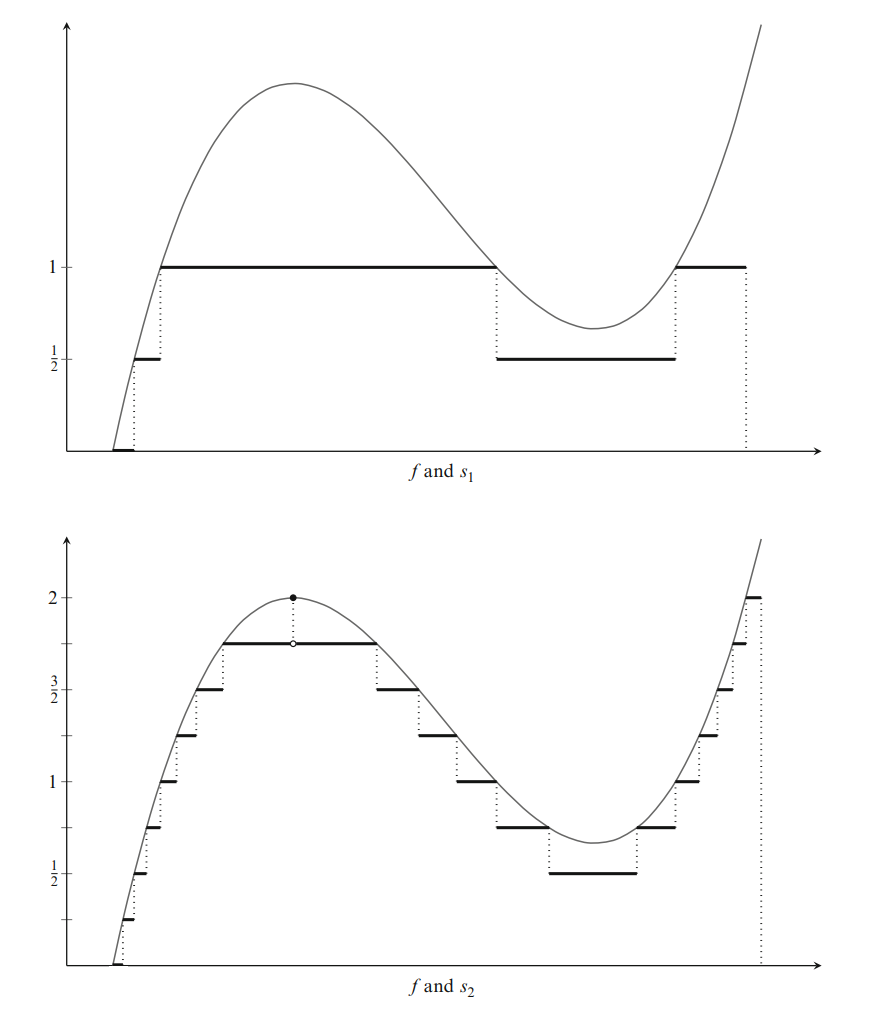
\includegraphics[width=0.8\textwidth]{simple_function.png}
    \caption{Example of simple functions $s_1$ and $s_2$(From \cite{27}).}
    \label{fig:simple_functions}
\end{figure}

\medskip

In the integration theory, we assume $\infty\cdot 0 = 0 \cdot \infty = 0$. And from now on, $(X,\mu,\mathfrak{M})$ is a measure space.

\medskip

\begin{definition}
If $s:X \to [0,\infty)$ is a simple function of the form 
\begin{align*}
    s = \sum^n_{i=1} \alpha_i \chi_{A_i},
\end{align*}
where $\alpha_i \neq \alpha_j$ for $i \neq j$, $A_i$ are pairwise disjoint measurable sets, then for any $E \in \mathfrak{M}$, we define
\begin{align*}
    \int_E s\, d\mu \coloneqq \sum^n_{i=1} \alpha_i \mu(A_i \cap E).
\end{align*}
Even if $\mu(A_i \cap E) = \infty$, but $\alpha_i = 0$, then $\alpha_i \cdot \mu(A_i \cap E) = 0$.
\end{definition}

\medskip

\begin{definition}
If $f:X \to [0,\infty]$ is measurable, and $E \in \mathfrak{M}$, we define the Lebesgue integral of $f$ over $E$ by
\begin{align*}
    \int_E f\,d\mu = \sup \int_E s\, d\mu,
\end{align*}
where the supremum is taken over all simple functions $s$ such that $0 \leq s \leq f$.
\end{definition}

\medskip

\begin{proposition}
Suppose $f,g:X \to [0,\infty]$ are measurable, and $A,B,E \in \mathfrak{M}$. Then,
\begin{enumerate}[label=(\alph*)]
    \item If $0 \leq f \leq g$, then $\int_E f\,d\mu \leq \int_E g\,d\mu$.
    
    \item If $A\subset B$ and $f \geq 0$, then $\int_A f\,d\mu \leq \int_B f\,d\mu$.
    
    \item If $f \geq 0$ and $c$ is a constant $0 \leq c < \infty$, then $\int_E cf\,d\mu = c \int_E f\,d\mu$.
    
    \item If $f(x) = 0$ for all $x \in E$, then $\int_E f\,d\mu = 0$ even if $\mu(E) = \infty$.
    
    \item If $\mu(E) = 0$, then $\int_E f\,d\mu = 0$ even if $f(x) = \infty$ for all $x\in E$.
    
    \item If $f \geq 0$, then $\int_E f\,d\mu = \int_X f \chi_E \,d\mu$.
\end{enumerate}
\end{proposition}

\medskip

\begin{lemma}\label{lemma_28}
Let $s$ and $t$ be nonnegative measurable simple functions $X$. Then the function
\begin{align*}
    \varphi(E)_s \coloneqq \int_E s\,d\mu, \quad E\in \mathfrak{M}
\end{align*}
defines a measure in $\mathfrak{M}$. Moreover,
\begin{align*}
    \int_X (s + t)\, d\mu = \int_X s\,d\mu + \int_X t\,d\mu.
\end{align*}
\end{lemma}
\begin{proof}
Denote $\varphi_s$ by $\varphi$. First, $\varphi(\emptyset) = 0$. Second, suppose $E_1, E_2, \cdots \in \mathfrak{M}$, $E_i \cap E_j = \emptyset$ for all $i \neq j$, then
\begin{align*}
    \varphi\left(\bigcup^\infty_{k=1} E_k\right) & = \int_{\bigcup E_k} s\, d\mu = \sum^n_{i=1} \alpha_i \mu \left(A_i \cap \bigcup^\infty_{k=1} E_k\right) = \sum^n_{i=1} \alpha_i \sum^\infty_{k=1} \mu(A_i \cap E_k) \\
    & = \sum^\infty_{k=1} \sum^n_{i=1} \alpha_i \mu(A_i \cap E_k) = \sum^\infty_{k=1} \int_{E_k} S\,d\mu = \sum^\infty_{k=1} \varphi(E_k),
    \end{align*}
which implies that $\varphi$ is countable additive. Therefore, $\varphi$ is a measure. 
    
It remains to prove that $\int_X (s + t)\, d\mu = \int_X s\,d\mu + \int_X t\,d\mu$, i.e. $\varphi_{s+t}(X) = \varphi_s(X) + \varphi_t(X)$. Since $s$ and $t$ are simple function, then they can be written in form
\begin{align*}
    s = \sum^n_{i=1} \alpha_i \chi_{A_i}, \quad t = \sum^m_{j=1} \beta_j \chi_{B_j}.
\end{align*}
Let $E_{ij} = A_i \cap B_j$, which are pairwise disjoint, then $s + t = \alpha_i + \beta_j$ on $E_{ij}$ and $X = \bigcup_{i,j} E_{ij}$. Now,
\begin{align*}
    \varphi_{s+t}(E_{ij}) = \int_{E_{ij}} (s + t)\,d\mu = (\alpha_i + \beta_j) \mu(E_{ij}) = \int_{E_{ij}}s\,d\mu + \int_{E_{ij}}t\,d\mu = \varphi_s(E_{ij}) + \varphi_t(E_{ij}),
\end{align*}
and hence
\begin{align*}
    \varphi_{s+t}(X) = \varphi_{s+t}\left(\bigcup_{i,j} E_{ij}\right) = \sum_{i,j} \varphi_{s+t}(E_{ij}) = \sum_{i,j}\varphi_s(E_{ij}) + \sum_{i,j}\varphi_t(E_{ij}) = \varphi_s(X) + \varphi_t(X),
\end{align*}
where we used the fact that $\varphi$ is countable additive.
\end{proof}

\medskip

The following theorem is one of the most important results of the theory of integration.

\medskip

\begin{theorem}[{\bf Lebesgue monotone convergence theorem}]\label{theorem_29}
Let $\{f_n\}$ be sequence of measurable functions on $X$ such that
\begin{enumerate}[label=(\alph*)]
    \item $0 \leq f_1 \leq f_2 \leq \cdots \leq \infty$ for every $x \in X$;
    
    \item $\lim_{n\to\infty} f_n(x) = f(x)$ for every $x \in X$.
\end{enumerate}
Then $f$ is measurable and 
\begin{align*}
    \lim_{n\to\infty} \int_X f_n\,d\mu = \int_X \lim_{n\to\infty}  f_n\,d\mu = \int_X f\,d\mu.
\end{align*}
\end{theorem}
\begin{proof}
Measurability of $f$ follows from Corollary \ref{coro_251}.

The sequence $\int_X f_n\,d\mu$ is increasing and hence it has a limit $\alpha = \lim_{n\to\infty} \int_X f_n\,d\mu$.\footnote{It may happen that the limit is infinity, but the limit exists.}Since $f_n \leq f$, then $\int_X f_n\,d\mu \leq \int_X f\,d\mu$ and hence $\alpha \leq \int_X f\,d\mu$. It remains to prove the opposite inequality. 
Let $0 \leq s \leq f$ be a simple function. Fix a constant $0 < c < 1$, and define
\begin{align*}
    E_n = \{x \in X \,:\, f_n(x) \geq cs(x)\}, \quad n = 1,2,3,\cdots
\end{align*}
Clearly, $E_1 \subset E_2 \subset \cdots$ and $\bigcup^\infty_{n=1} E_n = X$.\footnote{Indeed, for any $x \in X$, if $f(x) = 0$, then $f_n(x) = cs(x) = f(x) = 0$, and hence $x \in E_n$ for all $n$. If $f(x) > 0$, then $f(x) > cs(x)$. Since $f_n(x) \to f(x)$, then there is $n_0 > 0$ such that $f_n(x) > cs(x)$ for all $n \geq n_0$, and hence $x \in E_{n_0}$.}Then, we have
\begin{align*}
    \int_X f_n\,d\mu \geq \int_{E_n} f_n\,d\mu \geq c \int_{E_n} s\,d\mu.
\end{align*}
By Lemma \ref{lemma_28}, $\varphi(E) = \int_E s\, d\mu$ is a measure, and by Theorem \ref{theorem_16}(f), we have
\begin{align*}
    \int_{E_n} s\,d\mu = \varphi(E_n) \to \varphi\left(\bigcup^\infty_{n=1} E_n\right) = \varphi(X) = \int_X s\,d\mu.
\end{align*}
Then, letting $n \to \infty$ yields
\begin{align*}
    \alpha \leftarrow \int_X f_n\,d\mu \geq c \int_{E_n} s\,d\mu \to c\int_X s\,d\mu,
\end{align*}
then $\alpha \geq c\int_X s\,d\mu$. Therefore,
\begin{align*}
    \int_X f\,d\mu \geq \alpha \geq \int_X s\,d\mu,
\end{align*}
since $0 < c < 1$ is arbitrary. Taking supremum over all simple functions $0 \leq s \leq f$  yields
\begin{align*}
    \int_X f\,d\mu \geq \alpha \geq \int_X f\,d\mu,
\end{align*}
and thus $\alpha = \int_X f\,d\mu$.
\end{proof}

\medskip

\begin{lemma}
If $f,g: X \to [0,\infty]$ be measurable functions. Then,
\begin{align*}
    \int_X (f + g)\,d\mu = \int_X f\,d\mu + \int_X g\,d\mu.
\end{align*}
\end{lemma}
\begin{proof}
According to Theorem \ref{theorem_27}, there are increasing sequences $\{s_n\}, \{t_n\}$ of simple functions such that $s_n \to f$ and $t_n \to g$ for every point $x \in X$. Then, $0 \leq s_1 + t_1 \leq s_2 + t_2 \leq \cdots$, and $s_n + t_n$ converges pointwise to $f + g$.

By Lemma \ref{lemma_28}, for simple functions $s_n, t_n$,
\begin{align*}
    \int_X(s_n + t_n)\,d\mu = \int_X s_n\,d\mu + \int_X t_n\,d\mu,
\end{align*}
then, by Theorem \ref{theorem_29},
\begin{align*}
    \int_X(f + g)\,d\mu \leftarrow \int_X(s_n + t_n)\,d\mu = \int_X s_n\,d\mu + \int_X t_n\,d\mu \to \int_X f\,d\mu + \int_X g\,d\mu,
\end{align*}
which proves the lemma.
\end{proof}

\medskip

Applying an induction argument to this lemma, we obtain
\begin{align*}
    \int_X \sum^N_{n=1} f_n\,d\mu = \sum^N_{n=1}\int_X f_n\,d\mu.
\end{align*}

\medskip

\begin{theorem}\label{theorem_211}
If $f_n: X \to [0,\infty]$ are measurable functions for $n = 1,2,3,\cdots$, then for every $x \in X$,
\begin{align*}
    f(x) = \sum^\infty_{n=1} f_n(x)
\end{align*}
is measurable and 
\begin{align*}
    \int_X f\,d\mu = \int_X \sum^\infty_{n=1} f_n(x)\,d\mu = \sum^\infty_{n=1} \int_X f_n\,d\mu.
\end{align*}
\end{theorem}
\begin{proof}
Observe that $f$ is a limit of measurable functions, so $f$ is measurable. Indeed, $\sum^N_{n=1} f_n$ converges pointwise to $f$. Since $\sum^N_{n=1} f_n$ is an increasing sequence of measurables functions and it converges pointwise to $f$, by Theorem \ref{theorem_29}, we have
\begin{align*}
    \int_X f\,d\mu \xleftarrow[]{N \to \infty} \int_X \sum^N_{n=1} f_n\,d\mu = \sum^N_{n=1}\int_X f_n\,d\mu \xrightarrow[]{N \to \infty} \sum^\infty_{n=1}\int_X f_n\,d\mu,
\end{align*}
which proves the theorem.
\end{proof}

\medskip

\begin{theorem}[{\bf Fatou's lemma}]\label{theorem_212}
If $f_n: X \to [0,\infty]$ are measurable functions for $n = 1,2,3,\cdots$,\footnote{We do not assume that $f_n$ is convergent.}then
\begin{align*}
    \int_X \left(\liminf_{n\to\infty} f_n\right)\,d\mu \leq \liminf_{n\to\infty} \int_X f_n\,d\mu.
\end{align*}
\end{theorem}
\begin{proof}
Let $g_n = \inf\{f_n,f_{n+1},f_{n+1},\cdots\}$, by Theorem \ref{theorem_25}, $g_n$ are measurable. Clearly, $g_1 \leq g_2 \leq g_3 \cdots$ and $g_n$ converges pointwise to $\liminf_{n\to\infty} f_n$. Also, $g_n \leq f_n$ for all $n \in \mathbb{N}$, then
\begin{align*}
    \int_X g_n\,d\mu \leq \int_X f_n\,d\mu.
\end{align*}
Taking $\liminf$ on both sides gives
\begin{align}\label{theorem_212_equ_1}
    \liminf_{n\to\infty} \int_X g_n\,d\mu \leq \liminf_{n\to\infty} \int_X f_n\,d\mu,
\end{align}
since $g_n$ is increasing, then the left hand side equals to $\lim_{n\to\infty} \int_X g_n\,d\mu$. By the monotone convergence theorem \ref{theorem_29}, 
\begin{align*}
    \lim_{n\to\infty} \int_X g_n\,d\mu = \int_X \left(\liminf_{n\to\infty} f_n\right)\,d\mu,
\end{align*}
and thus, by \eqref{theorem_212_equ_1}, 
\begin{align*}
    \int_X \left(\liminf_{n\to\infty} f_n\right)\,d\mu \leq \liminf_{n\to\infty} \int_X f_n\,d\mu.
\end{align*}
\end{proof}

\medskip

\begin{remark}
In general, we do not have equality.
\end{remark}
\begin{proof}
Now we construct a sequence of measurable functions $f_n: \mathbb{R} \to [0,\infty]$ such that the inequality in Fatou’s lemma is strict.\footnote{Here is another simple example: Let $X = \mathbb{R}$, $E = [0,\infty)$ and let $f_n: E \to [0,\infty]$ be defined as for all $x \in E$, $f_n(x) = \chi_E$ if $n$ is even, and $f_n(x) = 1 - \chi_E$ if $n$ is odd. Then, $0 = \int_X \left(\liminf f_n\right)\,d\mu < \liminf \int_X f_n\,d\mu = n \cdot \frac{2}{n} = \infty$.}Let
\begin{align*}
    f_n(x) = \begin{cases}
        n, & -\frac{1}{n} \leq x \leq \frac{1}{n}, \\
        0, & \text{otherwise}.
    \end{cases}
\end{align*}
Then, we have 
\begin{align*}
    0 = \int_X \left(\liminf_{n\to\infty} f_n\right)\,d\mu < \liminf_{n\to\infty} \int_X f_n\,d\mu = n \cdot \frac{2}{n} = 2.
\end{align*}
\end{proof}

\medskip

\begin{theorem}\label{theorem_213}
Let $f: X \to [0,\infty]$ be measurable function. Then, for $E \in \mathfrak{M}$,
\begin{align}\label{theorem_213_equ1}
    \varphi(E) = \int_E f\,d\mu
\end{align}
defines a measure in $\mathfrak{M}$. Moreover, for every measurable function $g: X \to [0,\infty]$,
\begin{align}\label{theorem_213_equ2}
    \int_X g\,d\varphi = \int_X gf\, d\mu.
\end{align}
\end{theorem}

\begin{remark}
~\begin{enumerate}[label=(\alph*)]
    \item It is natural to think $d\varphi = f\,d\mu$ and regard $f\,d\mu$ as a measure.
    
    \item We already proved \eqref{theorem_213_equ1} when $f$ is a simple function in Lemma \ref{lemma_28}.
\end{enumerate}
\end{remark}

\medskip

\begin{proof}[Proof of Theorem \ref{theorem_213}]
Clearly, $\varphi(\emptyset) = 0$. To prove that $\varphi$ is a measure, it suffices to prove that $\varphi$ is countable additive. Let $E_1,E_2,\cdots \in \mathfrak{M}$ be pairwise disjoint and $E = \bigcup^\infty_{n=1} E_n$. Observe that
\begin{align*}
    \chi_E f = \sum^\infty_{n=1} \chi_{E_n}f,
\end{align*}
and by Theorem \ref{theorem_211}, we have
\begin{align*}
    \varphi(E) = \int_X \chi_Ef\,d\mu = \int_X \sum^\infty_{n=1} \chi_{E_n}f\,d\mu = \sum^\infty_{n=1} \int_X \chi_{E_n}f\,d\mu = \sum^\infty_{n=1} \varphi(E_n),
\end{align*}
which implies the countable additivity of $\varphi$. Hence, $\varphi$ is a measure.

Now it remains to prove that
\begin{align*}
    \int_X g\,d\varphi = \int_X gf\, d\mu.
\end{align*}
If $g = \chi_E, E \in \mathfrak{M}$, then
\begin{align*}
    \int_X g\,d\varphi = \int_X \chi_E\,d\varphi = \varphi(E) = \int_X \chi_Ef\,d\mu,
\end{align*}
which implies that \eqref{theorem_213_equ2} holds if $g = \chi_E$. Hence, it also holds for any simple functions, since simple function is a linear combination of the characteristic functions. If $g$ is any measurable function, then there are simple functions $0 \leq g_1 \leq g_2 \leq \cdots$ and $g_n \to g$, by the monotone convergence theorem \ref{theorem_29},
\begin{align*}
    \int_X g\,d\varphi \leftarrow \int_X g_n\,d\varphi = \int_X g_nf\,d\mu \to \int_X gf\,d\mu.
\end{align*}
\end{proof}

\medskip

Recall that $f^+ = \max\{f,0\}, f^- = - \min\{f,0\}$ are measurable, and $f^+$ and $f^-$ are called positive part and negative part of $f$. Also $f = f^+ + f^-, \left|f\right| = f^+ + f^-$.

If $f: X \to \overline{\mathbb{R}}$ is measurable and each of the integrals $\int_X f^+\,d\mu$ and $\int_X f^-\,d\mu$ is finite, then we define
\begin{align*}
    \int_X f\,d\mu = \int_X f^+\,d\mu - \int_X f^-\,d\mu.
\end{align*}

\medskip

Now we can extend the measurable function $f:X \to \overline{\mathbb{R}}$ to complex valued measurable function $f: X \to \mathbb{C}$.

\medskip

\begin{definition}\label{def_27}
Let $(X,\mathfrak{M},\mu)$ be a measurable space. The space $L^1(\mu)$ of all measurable function $f: X \to \mathbb{C}$ such that
\begin{align*}
    \left\|f\right\|_1 = \int_X \left|f\right|\,d\mu < \infty.
\end{align*}
Elements of $L^1(\mu)$ is called Lebesgue integral functions or summable functions.
\end{definition}

\medskip

If $f = u + iv$ is Lebesgue integral, then the functions $u^+, n^-, v^+, v^-$ are measurable and Lebesgue integral as bounded by $\left|f\right|$. For any $E \in \mathfrak{M}$, we define
\begin{align*}
    \int_E f\,d\mu = \left(\int_E u^+\,d\mu - \int_E u^-\,d\mu\right) + i \left(\int_E v^+\,d\mu - \int_E v^-\,d\mu\right).
\end{align*}

\medskip

\begin{theorem}
$L^1(\mu)$ is a linear space and if $\alpha,\beta \in \mathbb{C}$, then $\alpha f + \beta g \in L^1(\mu)$ and
\begin{align*}
    \int_X (\alpha f + \beta g)\,d\mu = \alpha \int_X f\,d\mu + \beta \int_X g\,d\mu.
\end{align*}
\end{theorem}

\medskip

\begin{remark}
In other words, $f \mapsto \int_X f\,d\mu$ is a linear functional in $L^1(\mu)$.
\end{remark}

\medskip

\begin{definition}
Similarly, we define $L^1(\mu,\mathbb{R}^n)$ be the class of all measurable functions $f = (f_1,\cdots,f_n): X \to \mathbb{R}^n$ such that
\begin{align*}
    \left\|f\right\|_1 = \int_X \left|f\right|\,d\mu < \infty.
\end{align*}
Then we define 
\begin{align*}
    \int_X f\,d\mu = \left(\int_X f_1\,d\mu,\cdots,\int_X f_n\,d\mu\right).
\end{align*}
\end{definition}

\medskip

\begin{theorem}\label{theorem_215}
If $f \in L^1(\mu,\mathbb{R}^n)$, then
\begin{align*}
    \left|\int_X f\,d\mu\right| \leq \int_X \left|f\right|\,d\mu.
\end{align*}
\end{theorem}
\begin{proof}
Let $\alpha = (\alpha_1,\cdots,\alpha_n) \in \mathbb{R}^n$ be a unit vector and $\left|\int_X f\,d\mu\right| = \left\langle \alpha,\int_X f\,d\mu \right\rangle$. Then, by Cauchy Schwarz inequality,
\begin{align*}
    \left|\int_X f\,d\mu\right| & = \left\langle \alpha,\int_X f\,d\mu \right\rangle = \sum^n_{i=1} \alpha_i \int_X f_i\,d\mu = \int_X \sum^n_{i=1} \alpha_i f_i\,d\mu = \int_X \left\langle \alpha,f\mu \right\rangle \leq \int_X \left|f\right|\,d\mu.
\end{align*}
\end{proof}

\medskip

\begin{theorem}[{\bf Lebesgue dominated convergence theorem}]
Suppose $\{f_n\}$ is a sequence of complex valued functions on $X$ such that $f_n$ converges pointwise to $f$ for every $x\in X$, that is $f(x) = \lim_{n\to\infty}f_n(x)$ for every $x\in X$. If there is a function $g \in L^1(\mu)$ ($g$ is real valued) such that $\left|f_n(x)\right| \leq g(x)$ for every $x \in X$ and all $n = 1,2,\cdots$, then $f \in L^1(\mu)$,
\begin{align*}
    \lim_{n\to\infty} \int_X \left|f - f_n\right|\,d\mu = 0,
\end{align*}
and
\begin{align*}
    \lim_{n\to\infty} \int_X f_n\,d\mu = \int_X f\,d\mu.
\end{align*}
\end{theorem}
\begin{proof}
Clearly, $f$ is measurable and $\left|f\right| \leq g$. Hence, $f \in L^1(\mu)$. Since $\left|f - f_n\right| \leq \left|f\right| + \left|f_n\right| \leq 2g$, then $2g - \left|f - f_n\right| \geq 0$. Also, 
\begin{align*}
    \int_X 2g\,d\mu = \int_X \lim_{n\to\infty} \left(2g - \left|f - f_n\right|\right)\, d\mu = \int_X \liminf_{n\to\infty} \left(2g - \left|f - f_n\right|\right)\, d\mu
\end{align*}
and by Fatou's lemma \ref{theorem_212}, we have
\begin{align*}
    \int_X 2g\,d\mu \leq \liminf_{n\to\infty} \int_X \left(2g - \left|f - f_n\right|\right)\, d\mu = \int_X 2g\,d\mu - \limsup_{n\to\infty} \int_X \left|f - f_n\right|\, d\mu.
\end{align*}
Since $\int_X 2g\,d\mu$ is finite, $\limsup_{n\to\infty} \int_X \left|f - f_n\right|\, d\mu \leq 0$, and this implies that
\begin{align*}
    \lim_{n\to\infty} \int_X \left|f - f_n\right|\, d\mu = 0.
\end{align*}

Now, by Theorem \ref{theorem_215}, we have
\begin{align*}
    \left|\int_X f\,d\mu - \int_X f_n\,d\mu\right| \leq \int_X \left|f - f_n\right|\, d\mu \to 0,
\end{align*}
and thus,
\begin{align*}
    \lim_{n\to\infty} \int_X f_n\,d\mu = \int_X f\,d\mu.
\end{align*}
\end{proof}

\medskip

\section{Almost everywhere}

\begin{definition}
Given measurable space $(X,\mathfrak{M},\mu)$, a property holds almost everywhere (a.e.) if there is a set $N \in \mathfrak{M}$, $\mu(N) = 0$ such that the property holds for all $x \in X \setminus N$.
\end{definition}

\medskip

\begin{example}
$f_n \to f$ a.e. if there is a set $N \in \mathfrak{M}$, $\mu(N) = 0$ such that $f_n(x) \to f(x)$ for all $x \in X \setminus N$.
\end{example}

\medskip

\begin{example}
$f = g$ a.e. if $f(x) = g(x)$ for all $x \in X \setminus N$, $N \in \mathfrak{M}$, $\mu(N) = 0$. Note that if $f = g$ a.e, then for every $E \in \mathfrak{M}$,
\begin{align*}
    \int_E f\,d\mu = \int_E g\,d\mu.
\end{align*}
Therefore from the point of view of the integration theory, functions which are equal a.e. cannot be distinguished.
\end{example}

\medskip

\begin{theorem}\label{theorem_215}
~\begin{enumerate}[label=(\alph*)]
    \item If $f: X \to [0,\infty]$ is measurable, $E \in \mathfrak{M}$ and $\int_E f\,d\mu = 0$, then $f = 0$ a.e. in $E$.
    
    \item If $f \in L^1(\mu)$ and $\int_E f\,d\mu = 0$ for every $E \in \mathfrak{M}$, then $f = 0$ a.e. in $X$.
\end{enumerate}
\end{theorem}
\begin{proof}
~\begin{enumerate}[label=(\alph*)]
    \item Let $A_n = \left\{x \in E \,:\, f(x) \geq 1/n \right\}$. Then,
    \begin{align*}
        0 \leq \frac{1}{n} \mu(A_n) \leq \int_{A_n} f\,d\mu \leq \int_E f\,d\mu = 0,
    \end{align*}
    which implies $\mu(A_n) = 0$. Therefore,
    \begin{align*}
        \mu\left(\{x \in E \,:\, f(x) > 0 \}\right) = \mu\left(\bigcup^\infty_{n=1} A_n \right) \leq \sum^\infty_{n=1} \mu(A_n) = 0.
    \end{align*}
    Hence, $f = 0$ a.e. in $E$.
    
    \item Let $f = u + iv$. Define $E = \{x \in X \,:\, u(x) \geq 0 \}$, then 
    \begin{align*}
        0 = \int_E f\,d\mu = \int_E u\,d\mu + i \int_E v\,d\mu = \int_X u^+\,d\mu + i \int_E v\,d\mu,
    \end{align*}
    which implies $u^+ = 0$ a.e. in $X$. Similarly, $u^-, v^+, v^- = 0$ a.e. in $X$. Thus, $f = (u^+ - u^-) + i(v^+ - v^-) = 0$ a.e. in $X$.
\end{enumerate}
\end{proof}

\begin{corollary}
If $f,g \in L^1(\mu)$ and for every $E \in \mathfrak{M}$, $\int_E f\,d\mu = \int_E g\,d\mu$, then $f = g$ a.e.
\end{corollary}
\begin{proof}
It follows from Theorem \ref{theorem_215}(b) applied to $f - g$.
\end{proof}

\medskip


Recall Definition \ref{def_19} that a measure $\mu$ is {\em complete} if every subset of a set of measure zero is measurable (and hence has measure zero). All the measures obtained through the Carathéodory construction are complete by Proposition \ref{prop_14}, e.g. the Hausforff measure and the Lebesgue measure are complete. However, the Lebesgue measure on $\mathfrak{B}(\mathbb{R}^n)$ is not complete, i.e. there are sets of Lebesgue measure zero that are not Borel, see Example \ref{example_32}. However, we can assume that any measure is complete, because we can add all subsets of sets of measure zero to the $\sigma$-algebra.

\medskip

\begin{theorem}{\rm \cite{2}}\label{theorem_218}
Let $(X,\mathfrak{M},\mu)$ be a measure space, let $\mathfrak{M}^*$ be a collection of all $E \subset X$ for which there exist sets $A, B \in \mathfrak{M}$ such that $A \subset E \subset B$ and $\mu(B\setminus A) = 0$ and define $\mu(E) = \mu(A)$ in this situation. Then $\mathfrak{M}^*$ is a $\sigma$-algebra and $\mu$ is a complete measure on $\mathfrak{M}^*$.
\end{theorem}

\medskip

\begin{definition}\label{def_210}
Suppose now that $(X,\mathfrak{M},\mu)$ is a complete space. $Y$ is any metric space, $N \in \mathfrak{M}$ and $\mu(N) = 0$. We say the function $f: X\setminus N \to Y$ is measurable if there is $y_0 \in Y$ such that
\begin{align*}
    \widetilde{f}(x) = \begin{cases}
        f(x), & x \in X \setminus N, \\
        y_0, & x \in N,
    \end{cases}
\end{align*}
is measurable. 
\end{definition}


It follows from the assumption that $\mu$ is complete, then if $\bar{f}(x): X \to Y$ is any function such that $\widetilde{f} = \bar{f}$ a.e., then $\bar{f}$ is measurable too. In particular, we can take $\bar{f}(x)$ as
\begin{align*}
    \bar{f}(x) = \begin{cases}
        f(x), & x \in X \setminus N, \\
        y, & x \in N,
    \end{cases}
\end{align*}
where $y$ is arbitrary.

Now if $f = g$ a.e., we write $f \sim g$. Clearly, $f \sim g$ is an equivalence relation. In particular functions in $L^1(\mu)$ need to be defined a.e. only. Since we identify functions in $L^1(\mu)$ that are equal a.e., we identify $L^1(\mu)$ with the quotient space $L^1(\mu)/\sim$. Therefore, $f \in L^1(\mu)$, $f = 0$ a.e. if and only if $\left\|f\right\| = \int_X|f|\,d\mu = 0$.

\medskip


\begin{theorem}[{\bf Lebesgue dominated convergence theorem}]\label{theorem_217}
Suppose that $\{f_n\}$ is a sequence of complex valued functions on $X$ defined a.e. If $f(x) = \lim_{n\to\infty} f_n(x)$ for almost all $x \in X$, and if there is a function $g \in L^1(\mu)$ such that $\left|f_n(x)\right| \leq g(x)$ for all $n = 1,2,3,\cdots$, then $f \in L^1(\mu)$,
\begin{align*}
    \lim_{n\to\infty} \int_X \left|f - f_n\right|\,d\mu = 0,
\end{align*}
and
\begin{align*}
    \lim_{n\to\infty} \int_X f_n\,d\mu = \int_X f\,d\mu.
\end{align*}
\end{theorem}

\medskip

Recall that if $Y$ is a metric space, then a mapping $f: X \to Y$ is Borel if it is measurable with respect to $\mathfrak{B}(X)$, that is for every open set $U \subset Y$, $f^{-1}(U) \in \mathfrak{B}(X)$. Since $\sigma$-algebra of Lebesgue measurable sets is larger, then not every Lebesgue measurable mapping $f: \mathbb{R}^n \to Y$ is Borel. However, we could have the following result.

\medskip

\begin{theorem}\label{theorem_220}
If $Y$ is a separable metric space and $f: \mathbb{R}^n \to Y$ is Lebesgue measurable, then there is a Borel mapping $g: \mathbb{R}^n \to Y$ such that $f = g$ a.e.
\end{theorem}
\begin{proof}
Since $Y$ is separable, then there is a countable family of open sets $\{U_i\}^\infty_{i=1}$ such that every open set in $Y$ is a union of open sets from this family. Indeed, it suffices to take the family of open balls with rational length radii and centers in a countable dense set in $Y$.

For $i = 1,2,3,\cdots$, let $M_i \subset \mathbb{R}^n$ be a $F_\sigma$ set such that 
\begin{align*}
    M_i \subset f^{-1}(U_i), \quad \mathcal{L}_n\left(f^{-1}(U_i) \setminus M_i\right) = 0,
\end{align*}
see Theorem \ref{theorem_124}(e). Let $E = \bigcup^\infty_{i=1} \left(f^{-1}(U_i) \setminus M_i\right)$, then clearly $E$ has Lebesgue measure zero and hence by Theorem \ref{theorem_124}(c), there is a $G_\delta$ set $H$ such that $E \subset H$ and $\mathcal{L}_n(H) = 0$. 

Now fix $y_0 \in Y$ and define 
\begin{align*}
    g(x) = \begin{cases}
        f(x), & x \notin H,\\
        y_0, & x \in H.
    \end{cases}
\end{align*}
Clearly $f = g$ a.e., because $f = g$ on $\mathbb{R}^n \setminus H$ and $\mathcal{L}_n(H) = 0$. 

It remains to prove that $g$ is Borel. It is easy to see that if $y_0 \notin U_i$, then $g^{-1}(U_i) = M_i \setminus H$, and if $y_0 \in U_i$, then $g^{-1}(U_i) = M_i \cup H$.\footnote{Drawing a picture would be clear.}In each case, $g^{-1}(U_i)$ is a Borel set. Since every open set $U \subset Y$ can be represented as $U = \bigcup^\infty_{j=1} U_{i_j}$, then the set 
$$g^{-1}(U) = \bigcup^\infty_{j=1} g^{-1}(U_{i_j})$$ 
is Borel.
\end{proof}

\medskip

\section{Theorems of Lusin and Egorov}

\begin{theorem}[{\bf Lusin}]
Let $X$ be a metric space and $\mu$ a measure in $\mathfrak{B}(X)$ such that $X$ is a union of countable many open sets of finite measure. Let $Y$ be a separable metric space, if $f: X \to Y$ is a Borel mapping, then for any $\varepsilon > 0$, there is a closed set $F \subset X$ such that $\mu(X \setminus F) < \varepsilon$ and $f|_{F}$ is continuous.
\end{theorem}
\begin{proof}
Since $X$ is a union of countable many open sets of finite measure, by Theorem \ref{theorem_114}, for any $E \in \mathfrak{B}(X)$,
\begin{align*}
    \mu(E) = \inf_{\substack{U \supset E\\ U \in \mathbb{R} - \text{open}}} \mu(U).
\end{align*}
In fact, we can choose $U$ such that $\mu(U \setminus E) < \varepsilon$. Indeed, $E = \bigcup^\infty_i E_i$, $\mu(E_i) < \infty$, and according to Theorem \ref{theorem_124}(b), let $V_i \supset E_i$ be open such that $\mu(V_i \setminus E_i) < \varepsilon/2^i$. Then, $E \subset \bigcup^\infty_{i=1} V_i \coloneqq V$, and $V \setminus E \subset \left(\bigcup_{i} V_i\right) \setminus \left(\bigcup_{i} E_i\right) \subset \bigcup_i(V_i \setminus E_i)$, and hence
\begin{align*}
    \mu(V \setminus E) \leq \sum^\infty_{i=1} \mu(V_i \setminus E_i) < \varepsilon.
\end{align*}

Let $\{U_i\}^\infty_{i=1}$ be a countable collection of open sets such that every open set in $Y$ is a union of open sets from this collection, that is for any open set $U \subset Y$, $U = \bigcup^\infty_{j=1}U_{i_j}$. For any open set $U_i \subset Y$, since $f$ is a Borel mapping, then there is open set $V_i \subset X$ such that
\begin{align*}
    f^{-1}(U_i) \subset V_i, \quad \mu\left(V_i\setminus f^{-1}(U_i)\right) < \frac{\varepsilon}{2^{i+1}}.
\end{align*}
Let
\begin{align*}
    E \coloneqq \bigcup^\infty_{i=1} \left(V_i\setminus f^{-1}(U_i)\right),
\end{align*}
and clearly, $\mu(E) < \varepsilon/2$. 

Now we want to prove that $g = f|_{X \setminus E}$ is continuous. Note that\footnote{Indeed, $g^{-1}(U_i) \subset f^{-1}(U_i) \subset V_i$, also since $g$ is defined on $X \setminus E$, then $g^{-1}(U_i) \subset X \setminus E$. Hence, $g^{-1}(U_i) \subset V_i \cap (X \setminus E)$. For the other direction, since $V_i\setminus f^{-1}(U_i) \subset E$ is a smaller set compared with $E$, $V_i \cap (X \setminus E) \subset V_i \cap \left(X \setminus (V_i\setminus f^{-1}(U_i))\right) = f^{-1}(U_i)$ (drawing a picture would yield the last equality). And since $f = g$ on $X \setminus E$, $V_i \cap (X \setminus E) \subset f^{-1}(U_i) \cap (X \setminus E) = g^{-1}(U_i)$. Thus, the equality holds.}
\begin{align*}
    g^{-1}(U_i) = V_i \cap (X \setminus E).
\end{align*}
In order to prove that $g$ is continuous, it suffices to prove that for every open set $U \subset Y$, there is an open set $V \subset X$ such that $g^{-1}(U) = V \cap (X \setminus E)$.\footnote{{\bf Theorem 4.8} in Rudin's {\em Principles of Mathematical Analysis}: A mapping $f$ of a metric space $X$ into a metric space $Y$ is continuous on $X$ if and only if $f^{-1}(V)$ is open in $X$ for every set $V$ in $Y$ \cite{28}. (Note that the class of open sets in the metric space $X \setminus E$ is exactly the class of sets of the form $V \cap (X \setminus E)$, where $V \subset X$ is open.)}Since $U = \bigcup^\infty_{j=1} U_{i_j}$, we have
\begin{align*}
    g^{-1}(U) = \bigcup^\infty_{j=1} g^{-1}(U_{i_j}) = \bigcup^\infty_{j=1}\left(V_{i_j} \cap (X \setminus E)\right) = \left(\bigcup^\infty_{j=1} V_{i_j} \right) \cap (X \setminus E),
\end{align*}
which proves the continuity of $g$ in $X \setminus E$. Again, by Theorem \ref{theorem_114}, there is an open set $G \subset X$ such that $E \subset G$ and $\mu(G \setminus E) < \varepsilon/2$. Then, 
\begin{align*}
    \mu(G) = \mu(E) + \mu(G \setminus E) < \varepsilon.
\end{align*}
Thus, $F = X \setminus G \subset X \setminus E$ is closed, which implies $f|_F$ is continuous, and $\mu(X \setminus F) = \mu(G) < \varepsilon$.
\end{proof} 

\medskip
As a corollary we will prove the following characterization of Lebesgue measurable functions also known as the Lusin theorem. Recall that let $E \subset \mathbb{R}^n$ be Lebesgue measurable, we say $f: E \to \mathbb{R}$ is Lebesgue measurable if $f^{-1}(U)$ is Lebesgue measurable for every open set $U \subset \mathbb{R}$.

\medskip

\begin{theorem}[{\bf Lusin}]
Let $E \subset \mathbb{R}^n$ be Lebesgue measurable. Then a function $f: E \to \mathbb{R}$ is Lebesgue measurable if and only if for any $\varepsilon > 0$, there is a closed set $F \subset E$ such that $f|_F$ is continuous and $\mathcal{L}_n(E \setminus F) < \varepsilon$.
\end{theorem}
\begin{proof}
~\begin{enumerate}
    \item[($\Rightarrow$)] By Theorem \ref{theorem_220}, there is a set $N \subset E$, $\mathcal{L}_n(N) = 0$ such that
    \begin{align*}
        \widetilde{f}(x) = \begin{cases}
            f(x), & x \in E \setminus N, \\
            y_0, & x \in N,
        \end{cases}
    \end{align*}
    is Borel. Observe that $f = \widetilde{f}$ a.e. By previous theorem, there is a closed set $\widetilde{F} \subset E$ such that $\mathcal{L}_n(E \setminus \widetilde{F}) < \varepsilon/2$ and $\widetilde{f}|_{\widetilde{F}}$ is continuous. Since $f = \widetilde{f}$ on $E \setminus N$, $f|_{\widetilde{F} \setminus N}$ is continuous.
    
    Also, $\mathcal{L}_n(N) = 0$, then $N$ is measurable, and hence there is an open set $G$ such that $N \subset G$ and $\mathcal{L}_n(G \setminus N) < \varepsilon/2$ (see Theorem \ref{theorem_124}(b)). Clearly, $f|_{\widetilde{F} \setminus G}$ is continuous, and $F \coloneqq \widetilde{F} \setminus G$ is closed. Observe that $E \setminus F = E \setminus (\widetilde{F} \setminus G) \subset ((E \setminus \widetilde{F}) \cup G)$, and then
    \begin{align*}
        \mathcal{L}_n(E \setminus F) \leq \mathcal{L}_n(E \setminus \widetilde{F}) + \mathcal{L}_n(G) < \varepsilon,
    \end{align*}
    also, we have $f|_F$ is continuous, hence this direction is proved.
    
    \item[($\Leftarrow$)] It suffices to prove that $E_a = \{x \in E \,:\, f(x) \geq a \}$ is Lebesgue measurable for any $a \in \mathbb{R}$ (see Theorem \ref{theprem_24}). By assumption, there is a closed subset $F_m \subset E$ such that $\mathcal{L}_n(E \setminus F_m) < 1/m$ and $f|_{F_m}$ is continuous. 
    
    Let $F_m' = \{x \in F_m \,:\, \left(f|_{F_m}\right)(x) \geq a \}$, and clearly, $F_m' = E_a \cap F_m$. Observe that $F_m'$ is closed, since $F_m$ is closed and $f|_{F_m}$ is continuous. Also, since $E_a \setminus F_m' = E_a \setminus F_m$ and $E_a \setminus F_m \subset E \setminus F_m$, we have
    \begin{align*}
        \mathcal{L}_n^*(E_a \setminus F_m') \leq \mathcal{L}_n^*(E \setminus F_m) < \frac{1}{m},
    \end{align*}
    which implies
    \begin{align*}
        \mathcal{L}_n^*\left(E_a \setminus \bigcup_m F_m'\right) = 0.
    \end{align*}
    Since
    \begin{align*}
        E_a = \underbrace{\left(E_a \setminus \bigcup_m F_m'\right)}_{\text{measure zero}}  \cup \underbrace{\left(\bigcup_m F_m'\right)}_{F_\sigma},
    \end{align*}
    then $E_a$ is measurable, which proves this direction.
\end{enumerate}
\end{proof}

\medskip

\begin{theorem}[{\bf Egorov}]\label{theorem_223}
Let $\mu$ be a complete finite measure on a set $X$. Let $f_n: X \to Y$ be a sequence of measurable mappings with values in a separable metric space $Y$. If $f_n \to f$ a.e., then $f$ is measurable and for any $\varepsilon > 0$, there is a measurable set $E \subset X$ such that $\mu(X \setminus E) < \varepsilon$ and $f_n$ uniformly converges to $f$ on $E$.
\end{theorem}
\begin{proof}
Measurability of $f$ follows from Theorem \ref{theorem_26}.\footnote{Now we show how to transfer from $f_n \to f$ everywhere to $f_n \to f$ almost everywhere. $f_n \to f$ a.e. means that $f_n(x) \to f(x)$ for $x \in X \setminus N$, $\mu(N) = 0$. Then, $\widetilde{f}_n \to \widetilde{f}$ everywhere, where
\begin{align*}
    \widetilde{f}_n(x) = \begin{cases}
        f_n(x), & x \in X \setminus N,\\
        y_0, & x \in N,
    \end{cases} \quad 
    \widetilde{f}(x) = \begin{cases}
        f(x), & x \in X \setminus N,\\
        y_0, & x \in N.
    \end{cases}
\end{align*}
Since $f_n$ is measurable, by Definition \ref{def_210}, $\widetilde{f}_n$ is measurable. Also, $\widetilde{f}_n \to \widetilde{f}$ everywhere, and then $\widetilde{f}$ is measurable. Since $\widetilde{f}$ and $f$ differ on a set of measure zero, $f$ is measurable.}Let
\begin{align*}
    C_{i,j} = \bigcup^\infty_{n=j} \left\{x \in X \,:\, d(f_n(x),f(x)) \geq \frac{1}{2^i}\right\}.
\end{align*}
We want to prove that $C_{i,j}$ is measurable. First, observe that the mapping $F \coloneqq (f_n,f): X \to Y \times Y$ is measurable. Indeed, if $\{U_i\}^\infty_{i=1}$ is a countable base of open sets in $Y$, that is every open set in $Y$ is a countable union of open sets from $\{U_i\}$. Then, $\{U_i \times U_j\}_{i,j}$ is a countable base of open sets in $Y \times Y$. Therefore,
\begin{align*}
    F^{-1}(U_i \times U_j) = f_n^{-1}(U_i) \cup f^{-1}(U_j),
\end{align*}
which is measurable, since $f_n, f$ are measurable. Every open set $U \subset Y \times Y$ can be written as $U = \bigcup^\infty_{k=1} U_{i_k} \times U_{j_k}$, then
\begin{align*}
    F^{-1}(U) = \bigcup^\infty_k F^{-1}\left(U_{i_k} \times U_{j_k}\right),
\end{align*}
which is measurable. Hence, $F$ is measurable.

Now, $d: Y \times Y \to \mathbb{R}$ is continuous, by Theorem \ref{theorem_21}, $d \circ F: X \to \mathbb{R}$ defined as $d\circ F(x) = d(f_n(x),f(x))$ is measurable. Hence,
\begin{align*}
    \left\{x \in X \,:\, d(f_n(x),f(x)) \geq \frac{1}{2^i}\right\} & = F^{-1} \left\{(y_1,y_2) \in Y \times Y \,:\, d(y_1,y_2) \geq \frac{1}{2^i}\right\} \\
    & = F^{-1} \left(d^{-1}([2^{-i},\infty))\right) \\
    & = (d \circ F)^{-1} ([2^{-i},\infty))
\end{align*}
is measurable, and therefore $C_{i,j}$ is measurable. 

Observe that for fixed $i$, $C_{i,1} \supset C_{i,2} \supset C_{i,3} \supset \cdots$ is a decreasing sequence of sets. Also, $\mu(C_{i,1}) < \mu(X) < \infty$, and then by Theorem \ref{theorem_16}(g), we have
\begin{align}\label{theorem_223_equ1}
    \lim_{j\to\infty} \mu\left(C_{i,j}\right) = \mu \left(\bigcap^\infty_{j=1} C_{i,j}\right) = 0.
\end{align}
Indeed, the intersection has measure zero because if $x \in \bigcap^\infty_{j=1} C_{i,j}$, then
\begin{align*}
    x \in \bigcap^\infty_{j=1} \bigcup^\infty_{n=j} \left\{x \in X \,:\, d(f_n(x),f(x)) \geq \frac{1}{2^i}\right\},
\end{align*}
which implies for all $j$, there exists $n \geq j$ such that $d(f_n(x),f(x)) \geq 2^{-i}$. And this means that $f_n$ does not converge to $f$, and this can only happen in a set of measure zero according to the definition of $f_n$.

Now it follows from \eqref{theorem_223_equ1} that for every $i \in \mathbb{N}$, there is an integer $J(i)$ such that $\mu(C_{i,J(i)}) < \varepsilon/2^i$. Clearly, 
\begin{align*}
    \mu\left(\bigcup^\infty_{i=1} C_{i,J(i)}\right) < \varepsilon.
\end{align*}

Let $E = X \setminus \bigcup^\infty_{i=1} C_{i,J(i)}$, and clearly $\mu(X \setminus E) < \varepsilon$. It remains to prove that $f_n$ converges uniformly on $E$. Take any $i$, let $n \geq J(i)$ and $x \in E$ be arbitrary. Then, 
\begin{align*}
    x \notin C_{i,J(i)} & = \bigcup^\infty_{k=J(i)} \left\{x \in X \,:\, d(f_k(x),f(x)) \geq \frac{1}{2^i} \right\} \\
    & = \bigcap^\infty_{k=J(i)} \left\{x \in X \,:\, d(f_k(x),f(x)) < \frac{1}{2^i} \right\}.
\end{align*}
Since $n \geq J(i)$, $d(f_n(x),f(x)) < 2^{-i}$. Now we have for all $i \in \mathbb{N}$ and all $n \geq J(i)$, take any $x \in E$, and we have $d(f_n(x),f(x)) < 2^{-i}$, which proves the uniform convergence of $f_n$.
\end{proof}

\medskip

\begin{remark}
This theorem does not hold if $\mu(X) = \infty$. $(X,\mathfrak{M},\mu)$ is an arbitrary measure space, in Lusin theorem, it requires $X$ to be a metric space. Also, $\mu$ need to be complete in order to talk about almost everywhere (see Theorem \ref{theorem_218}). In particular, if $f$ is measurable, $\widetilde{f} = f$ a.e., then $\widetilde{f}$ is measurable.
\end{remark}

\medskip

\begin{remark}
If $X$ is a metric space, $\mu$ is a measure on Borel set and $\mu(X) < \infty$, then we can take $E$ to be closed. 
\end{remark}

\medskip

\section{Convergence in measure}

\begin{definition}
We say a sequence of measurable functions $f_n: X \to \mathbb{R}$ converges in measure to a measurable function $f: X \to \mathbb{R}$ if for every $\varepsilon > 0$,
\begin{align*}
    \lim_{n\to\infty} \mu\left(\{x \in X \,:\, \left|f_n(x) - f(x)\right| \geq \varepsilon\} \right) = 0.
\end{align*}
We denote the convergence in measure by $f_n \xrightarrow[]{\mu} f$. In general, we assume that the functions $f_n$ and $f$ are defined a.e.
\end{definition}

\medskip

\begin{theorem}[{\bf Lebesgue}]
If $\mu(X) < \infty$ and a sequence of measurable functions $f_n: X \to \mathbb{R}$ converges to $f: X \to \mathbb{R}$ a.e., then it converges in measure, $f_n \xrightarrow[]{\mu} f$.
\end{theorem}
\begin{proof}
Given $\varepsilon > 0$, let $E_i = \{x \in X \,:\, \left|f_i(x) - f(x)\right| \geq \varepsilon\}$. The family of set $\bigcup^\infty_{i=n} E_i$ is a decreasing sequence of sets of finite measure, since $\mu(X) < \infty$ and hence
\begin{align*}
    \mu\left(\bigcup^\infty_{i=n} E_i\right) \to \mu\left(\bigcap^\infty_{n=1} \bigcup^\infty_{i=n} E_i\right) = 0.
\end{align*}
Indeed, if $x \in \bigcap^\infty_{n=1} \bigcup^\infty_{i=n} E_i$, then for all $n \in \mathbb{N}$, there is $i \geq n$ such that $\left|f_i(x) - f(x)\right| \geq \varepsilon$, which implies $f_i(x)$ does not converge to $f(x)$, and the set of such points has measure zero, since $f_n \to f$ a.e. Hence,
\begin{align*}
    \mu\left(\{x \in X \,:\, \left|f_n(x) - f(x)\right| \geq \varepsilon\}\right) = \mu(E_n) \leq \mu\left(\bigcup^\infty_{i=n} E_i\right) \to 0,
\end{align*}
which proves the convergence in measure.
\end{proof}

\medskip

\begin{theorem}[{\bf Riesz}]\label{theorem_225}
If $f_n \xrightarrow[]{\mu} f$, then there is a subsequence $f_{n_k}$ such that $f_{n_k} \xrightarrow[]{\mu} f$ a.e.
\end{theorem}
\begin{proof}
Since $f_n \xrightarrow[]{\mu} f$, then for every $i \in \mathbb{N}$, 
\begin{align*}
    \lim_{i\to\infty}\mu\left(\left\{x \,:\, \left|f_n(x) - f(x)\right| \geq \frac{1}{i} \right\}\right) = 0,
\end{align*}
which implies for every $i$, there is $N_i$ such that for all $n \geq N_i$,
\begin{align*}
    \mu\left(\left\{x \,:\, \left|f_n(x) - f(x)\right| \geq \frac{1}{i} \right\}\right) \leq \frac{1}{2^i}.
\end{align*}
We can take $n_1 < n_2 < n_3 < \cdots$. Let 
\begin{align*}
    F_k = X \setminus \bigcup^\infty_{i=k} \left\{x \,:\, \left|f_{n_i}(x) - f(x)\right| \geq \frac{1}{i} \right\}.
\end{align*}

We claim $f_{n_i}$ uniformly converges to $f$ on $F_k$. Indeed, if $x \in F_k$, then
\begin{align*}
    x \in \bigcap^\infty_{i=k} \left(X \setminus \left\{\left|f_{n_i}(x) - f(x)\right| \geq \frac{1}{i} \right\}\right),
\end{align*}
that is $x \in \bigcap^\infty_{i=k} \{\left|f_{n_i}(x) - f(x)\right| < 1/i \}$. Hence, for all $x \in F_k$, for all $i \geq k$, we have
\begin{align*}
    \left|f_{n_i}(x) - f(x)\right| \leq \frac{1}{i},
\end{align*}
which proves the uniform convergence of $f_{n_i}$ to $f$ on $F_k$.

It remains to show that $\mu\left(X \setminus \bigcup^\infty_{k=1} F_k \right) = 0$. Clearly, 
\begin{align*}
    \mu(X \setminus F_n) \leq \sum^\infty_{i=n} 2^{-i} = \frac{1}{2^{n-1}},
\end{align*}
and hence
\begin{align*}
    \mu\left(X \setminus \bigcup^\infty_{k=1} F_k \right) \leq \mu(X \setminus F_n) \leq \frac{1}{2^{n-1}} \xrightarrow[]{n \to \infty} 0.
\end{align*}
\end{proof}

\begin{remark}
In this theorem, the measure of the space can be infinite, $\mu(X) = \infty$. Also, we actually proved not only convergence a.e. but also uniform convergence
on subsets of $X$ whose complement has arbitrary small measure. Note that Lebesgue theorem combined with this stronger conclusion of Riesz theorem implies Egorov
theorem for sequences of real valued functions.
\end{remark}

\medskip

\begin{theorem}\label{theorem_226}
If $f_n, f \in L^1(\mu)$ and $\int_X \left|f_n - f\right|\,d\mu \to 0$, then $f_n \xrightarrow[]{\mu} f$.
\end{theorem}
\begin{proof}
Observe that $\varepsilon \chi_{\{x \,:\, \left|f_n - f\right| \geq \varepsilon\}} \leq \left|f_n - f\right|$, and taking integral on both sides yields
\begin{align*}
    \varepsilon \mu(\{x \,:\, \left|f_n - f\right| \geq \varepsilon\}) \leq \int_X \left|f_n - f\right| \, d\mu \to 0.
\end{align*}
Hence, $\mu(\{x \,:\, \left|f_n - f\right| \geq \varepsilon\}) \to 0$, which proves the convergence in measure.
\end{proof}

\medskip

\section{Absolute continuity of the integral}

The following result is known as the absolute continuity of the integral.

\medskip

\begin{theorem}\label{theorem_227}
Let $f \in L^1(\mu)$. Then for any $\varepsilon > 0$, there is $\delta > 0$ such that if $\mu(E) < \delta$,
\begin{align*}
    \int_E \left|f\right|\,d\mu < \varepsilon.
\end{align*}
\end{theorem}
\begin{proof}
Suppose to the contrary that there is $\varepsilon > 0$ and for all $\delta > 0$, there is $E \in \mathfrak{M}$ and $\mu(E) < \delta$ such that $\int_E \left|f\right|\,d\mu \geq \varepsilon$. Fix such $\varepsilon$, for $\delta = 1/2^n$, we can find $E_n \in \mathfrak{M}$ such that $\mu(E_n) < 1/2^n$ and $\int_{E_n} \left|f\right|\,d\mu \geq \varepsilon$. 

Let $A_k = \bigcup^\infty_{n=k} E_n$, which is a decreasing sequence of sets. For every $n$,
\begin{align*}
    \mu\left(\bigcap^\infty_{k=1} A_k\right) \leq \mu(A_n) \leq \sum^\infty_{i=n} \mu(E_i) \leq \sum^\infty_{i=n} \frac{1}{2^i} = \frac{1}{2^{n-1}},
\end{align*}
and since it holds for all $n$, then we have
\begin{align}\label{theorem_227_equ1}
    \mu\left(\bigcap^\infty_{k=1} A_k\right) = 0.
\end{align}

Recall that $\varphi(E) = \int_E \left|f\right|\,d\mu$ defines a measure in $\mathfrak{M}$, see Theorem \ref{theorem_213}, and since $f \in L^1(\mu)$,
\begin{align*}
    \varphi(A_1) = \int_{A_1} \left|f\right|\,d\mu \leq \int_X \left|f\right|\,d\mu < \infty.
\end{align*}
Now by Theorem \ref{theorem_16}(g) and \eqref{theorem_227_equ1},
\begin{align*}
    \lim_{n\to\infty} \varphi(A_n) = \varphi\left(\bigcap^\infty_{k=1} A_k\right) = \int_{\bigcap^\infty_{k=1} A_k} \left|f\right|\,d\mu = 0.
\end{align*}
On the other hand,
\begin{align*}
    \varphi(A_n) \geq \varphi(E_n) = \int_{E_n} \left|f\right|\,d\mu \geq \varepsilon,
\end{align*}
which is a contradiction.
\end{proof}

\medskip

\begin{definition}
We say that a family of functions $\mathcal{F} \subset L^1(\mu)$ is uniformly integrable (or equiintegrable) if for any $\varepsilon > 0$, there is $\delta > 0$ such that for all $f \in \mathcal{F}$ and all $E \in \mathfrak{M}$, if $\mu(E) < \delta$, then
\begin{align*}
    \int_E \left|f\right|\,d\mu < \varepsilon.
\end{align*}
\end{definition}

\medskip

\begin{theorem}\label{theorem_228}
If $f_n, f \in L^1(\mu)$ and $\lim_{n\to\infty}\int_X \left|f_n - f\right|\,d\mu = 0$, then the family $\{f_n\}^\infty_{n=1}$ is uniformly integrable.
\end{theorem}
\begin{proof}
Given $\varepsilon > 0$ and let $n_0$ be such that for $n > n_0$,
\begin{align*}
    \int_X \left|f_n - f\right|\,d\mu < \frac{\varepsilon}{2}.
\end{align*}
Let $\delta > 0$ be such that for $\mu(E) < \delta$,\footnote{This is possible since $f_n,f \in L^1(\mu)$ and the rest follows from Theorem \ref{theorem_227}.}
\begin{align*}
    \int_E \left|f\right| + \left|f_1\right| + \cdots + \left|f_{n_0}\right|\,d\mu < \frac{\varepsilon}{2}.
\end{align*}
If $\mu(E) < \delta$, then for any $n$, if $n \leq n_0$, then $\int_E \left|f_n\right|\,d\mu < \varepsilon$; if $n > n_0$, then
\begin{align*}
    \int_E \left|f_n\right|\,d\mu \leq \int_E \left|f_n - f\right|\,d\mu + \int_E \left|f\right|\,d\mu < 2 \cdot \frac{\varepsilon}{2} = \varepsilon,
\end{align*}
which proves that $\{f_n\}$ is uniformly integrable.
\end{proof}

\medskip

\begin{theorem}[{\bf Vitali}]
If $\mu(X) < \infty$ and $f,f_n \in L^1(\mu)$, then $\lim_{n\to\infty}\int_X \left|f_n - f\right|\,d\mu = 0$ if and only if $f_n \xrightarrow[]{\mu} f$ and $\{f_n\}^\infty_{n=1}$ is uniformly integrable.
\end{theorem}
\begin{proof}
~\begin{enumerate}
    \item[($\Rightarrow$)] This direction is obvious by Theorem \ref{theorem_226} and  \ref{theorem_228}.
    
    \item[($\Leftarrow$)] Suppose to the contrary that there is a subsequence $f_{n_k}$ and $\varepsilon > 0$ such that
    \begin{align}\label{theorem_229_equ1}
        \int_X \left|f_{n_k} - f\right|\,d\mu \geq \varepsilon.
    \end{align}
    By the Riesz theorem \ref{theorem_225}, we can further assume that $f_{n_k} \to f$ a.e. Let $\delta > 0$ be such that for all $n$, if $\mu(E) < \delta$,\footnote{This is possible since $f \in L^1(\mu)$ and $\{f_n\}$ is uniformly integrable.}
    \begin{align*}
        \int_E \left|f\right| + \left|f_n\right| \, d\mu < \frac{\varepsilon}{2}.
    \end{align*}
    By the Egorov theorem \ref{theorem_223}, there is a set $F \in \mathfrak{M}$ such that $\mu(X \setminus F) < \delta$ and $f_{n_k}$ uniformly converges to $f$ on $F$. Therefore, 
    \begin{align*}
        \int_X \left|f_{n_k} - f\right|\,d\mu & = \int_F \left|f_{n_k} - f\right|\,d\mu + \int_{X \setminus F} \left|f_{n_k} - f\right|\,d\mu \\
        & \leq \int_F \left|f_{n_k} - f\right|\,d\mu + \int_{X \setminus F} \left|f_{n_k}\right| + \left|f\right|\,d\mu < \varepsilon,
    \end{align*}
    for $k$ large enough, which is a contradiction to \eqref{theorem_229_equ1}. 
\end{enumerate}
\end{proof}



\medskip


\chapter{$L^p$-space}

\section{The $L^p$-spaces and inequalities}

In Definition \ref{def_27}, we talked about $L^1(\mu)$ space. Now we talk more about $L^p$ spaces.

\medskip

\begin{definition}
Let $(X, \mathfrak{M}, \mu)$ be measure space and $0 < p < \infty$. Denote $\widetilde{L}^p(\mu)$ the class of all measurable functions $f: X \to \mathbb{R}$ such that
\begin{align*}
    \left\|f\right\|_p = \left(\int_X \left|f\right|^p\, d\mu \right)^{1/p} < \infty.
\end{align*}
The space $L^p(\mu) = \widetilde{L}^p(\mu) / \sim$ is defined as the equivalence classes of measurable functions in $\widetilde{L}^p(\mu)$, where $f \sim g$ if and only if $f = g$ a.e. 
\end{definition}

\medskip

\begin{definition}
$\widetilde{L}^\infty (\mu)$ is the class of essentially bounded functions, i.e, $f \in \widetilde{L}^\infty (\mu)$ if there exists $M > 0$ such that $\left|f\right| \leq M$ a.e. Such smallest $M$ is denoted by $\left\|f\right\|_{\infty}$ and it is called essential supremum of $f$.\footnote{In other book\cite{33}, {\em essential supremum} of $f$ on $X$ is defined as 
\begin{align*}
    \operatorname{ess~sup}_X f = \inf \{M \in \mathbb{R} \,:\, \mu(\{x \,:\, f(x) > M\}) = 0\}.   
\end{align*}
Equivalently, 
\begin{align*}
    \operatorname{ess~sup}_X f =\inf \left\{\sup_X g \,:\, g = f \,\,\text{pointwise a.e.} \right\}.   
\end{align*}
And $\left\|f\right\|_{\infty}$ is defined as $\operatorname{ess~sup}_X \left|f\right|$.
}
\end{definition}

\medskip

Usually, $f \in L^p(\mu), 0 < p < \infty$ are complex valued, but sometimes we also consider $L^p(\mu)$ for real valued functions.

\medskip

\begin{exercise}
Prove the existence of essential supremum.
\end{exercise}
\begin{proof}
Let $S$ be the set of all real $\alpha$ such that
\begin{align*}
    \mu\left(g^{-1}((\alpha,\infty])\right) = 0.
\end{align*}
Let $M = \inf S$, since
\begin{align*}
    g^{-1} ((M,\infty]) = \bigcup^\infty_{n=1} g^{-1} \left(\left(M + \frac{1}{n},\infty\right]\right),
\end{align*}
and the countable union of sets with measure zero has measure zero, we see that $M \in S$.
\end{proof}

\medskip

\begin{example}
Function $f: \mathbb{N} \to \mathbb{C}$ can be identified with sequences $\{x_n\}^\infty_{n=1}$. Let $\mu$ be a counting measure on $\mathbb{N}$. Then, for $x = \{x_n\}^\infty_{n=1}$,
\begin{align*}
    L^p(\mu) = \left\{x \,:\, \left(\sum^\infty_{n=1} \left|x_n\right|^p \right)^{1/p} < \infty \right\},
\end{align*}
we write this sequence space as $\ell^p(\mathbb{N})$ with norm
\begin{align*}
    \left\|x\right\|_{\ell^p} = \left(\sum^\infty_{n=1} \left|x_n\right|^p \right)^{1/p}.
\end{align*}
Similarly, $\ell^\infty(\mathbb{N})$ is defined as
\begin{align*}
    \ell^\infty(\mathbb{N}) = L^\infty(\mu) = \left\{x \,:\, \sup \left|x_n\right| < \infty \right\}.
\end{align*}
\end{example}

\medskip

\begin{theorem}[{\bf Jensen's inequality}]
Let $(X,\mathfrak{M},\mu)$ be a measure space and $\mu(X) = 1$ ($\mu$ is a probability measure). If $f \in L^1(\mu)$, $a < f(x) < b$ a.e. and $\varphi$ is convex on $(a,b)$, then 
\begin{align*}
    \varphi \left(\int_X f\,d\mu\right) \leq \int_X \varphi \circ f \,d\mu.
\end{align*}
We allow $a = - \infty$ and $b = + \infty$.
\end{theorem}

\begin{remark}
For general finite measure $0 < \mu(X) < \infty$, then
\begin{align*}
    \varphi \left(\frac{1}{\mu(X)}\int_X f\,d\mu\right) \leq \frac{1}{\mu(X)} \int_X \varphi \circ f \,d\mu,
\end{align*}
since $\frac{d\mu}{\mu(X)} = d\nu$ is a probability measure.
\end{remark}

To prove this theorem, we need two facts about convex function, see Exercise 23, Chapter 4 in Rudin's {\em Principles of Mathematical Analysis}. If $f$ is convex on $(a,b)$, then
\begin{enumerate}[label=(\alph*)]
    \item $f$ is continuous on $(a,b)$.
    
    \item If $a < s < t < u < b$, then
    \begin{align*}
        \frac{f(t) - f(s)}{t - s} \leq \frac{f(u) - f(s)}{u - s} \leq \frac{f(u) - f(t)}{u - t}.
    \end{align*}
\end{enumerate}

\begin{proof}
Let $t = \int_X f\,d\mu$, then $a < t < b$. Let
\begin{align*}
    \beta \coloneqq \sup_{a < s < b} \frac{\varphi(t) - \varphi(s)}{t - s}.
\end{align*}
Clearly, $\beta \leq \frac{\varphi(u) - \varphi(t)}{u - t}$ for $t < u < b$ and $\beta \geq \frac{\varphi(t) - \varphi(s)}{t - s}$ for $a < s < t$, which implies
\begin{align*}
    \varphi(u) & \geq \varphi(t) + \beta(u - t), \\
    \varphi(s) & \geq \varphi(t) + \beta(s - t).
\end{align*}
This means that for all $a < s < b$, $\varphi(s) \geq \varphi(t) + \beta(s - t)$. 

Let $s = f(x)$, then $\varphi(f(x)) \geq \varphi(t) + \beta (f(x) - t)$, and hence
\begin{align*}
    \int_X \left(\varphi(f(x)) - \varphi(t) - \beta (f(x) - t)\right)\,d\mu \geq 0.
\end{align*}
Since $\mu(X) = 1$ and $t = \int_X f\,d\mu$ is a constant, integrating both sides of the above equation yields
\begin{align*}
    \int_X \varphi(f(x))\,d\mu - \varphi\left(\int_X f\,d\mu\right) - \beta \left(\int_X \varphi(f(x))\,d\mu - \int_X \varphi(f(x))\,d\mu\right) \geq 0,
\end{align*}
which implies
\begin{align*}
    \int_X \varphi(f(x))\,d\mu - \varphi\left(\int_X f\,d\mu\right) \geq 0.
\end{align*}
\end{proof}

\medskip

\begin{definition}
If $1 < p,q < \infty$, $1/p + 1/q = 1$ or if $p = 1, q = \infty$, then we say $p$ and $q$ are Hölder conjugate exponents. 
\end{definition}

\medskip

\begin{theorem}[{\bf Hölder's inequality}]\label{theorem_42}
Let $(X,\mathfrak{M},\mu)$ be a measure space and let $p, q$ be Hölder conjugate, for any measurable functions $f$ and $g$,
\begin{align*}
    \int_X \left|fg\right|\,d\mu \leq \left\|f\right\|_p \left\|g\right\|_q, 
\end{align*}
where $\left\|f\right\|_p = \left(\int_X \left|f\right|^p \,d\mu\right)^{1/p}$.
\end{theorem}

We need the following lemma to prove this theorem.

\begin{lemma}[{\bf Young's inequality}]\label{lemma_41}
If $a, b > 0$ and $p, q$ are Hölder conjugate, then
\begin{align}\label{lemma_41_equ1}
    ab \leq \frac{a^p}{p} + \frac{b^q}{q},
\end{align}
and equality hold if $a^p = b^q$.
\end{lemma}
\begin{proof}
There exist unique $s,t \in \mathbb{R}$ such that $a = e^{s/p}$ and $b = e^{t/q}$. By convexity of the function $e^x$,\footnote{For $\lambda \in (0,1)$, $e^{\lambda s + (1-\lambda)t} \leq \lambda e^s + (1-\lambda) e^t$. Now let $p = 1/\lambda$ and $q = 1/(1-\lambda)$, then the equivalence is easy to see.}
\begin{align*}
    e^{\frac{s}{p}+\frac{t}{q}} \leq \frac{1}{p} e^s + \frac{1}{q} e^t,
\end{align*}
which is equivalent to \eqref{lemma_41_equ1}.
\end{proof}

\begin{proof}[Proof of Theorem \ref{theorem_42}]
We can assume $0 \leq \left\|f\right\|_p < \infty$ and $0 \leq \left\|g\right\|_q < \infty$, since otherwise the inequality easily holds. By Young's inequality,
\begin{align*}
    \frac{\left|fg\right|}{\left\|f\right\|_p \left\|g\right\|_q} \leq \frac{1}{p} \left(\frac{\left|f\right|}{\left\|f\right\|_p}\right)^p + \frac{1}{q} \left(\frac{\left|g\right|}{\left\|g\right\|_q}\right)^q.
\end{align*}
Integrating the both sides of the above inequality yields
\begin{align*}
    \int_X \left|fg\right|\,d\mu \leq \left\|f\right\|_p \left\|g\right\|_q \left(\frac{1}{p\left\|f\right\|_p^p} \int_X \left|f\right|^p\,d\mu + \frac{1}{q\left\|g\right\|_q^q} \int_X \left|g\right|^q\,d\mu \right) = \left\|f\right\|_p \left\|g\right\|_q \left(\frac{1}{p} + \frac{1}{q}\right),
\end{align*}
which proves the inequality.
\end{proof}

\medskip

\begin{theorem}[{\bf Minkowski's inequality}]\label{theorem_43}
Let $(X,\mathfrak{M},\mu)$ be a measure space and $0 < p < \infty$. Then for any measurable functions $f,g$, we have
\begin{align}\label{theorem_43_equ1}
    \left\|f+g\right\|_p \leq \left\|f\right\|_p + \left\|g\right\|_p.
\end{align}
\end{theorem}
\begin{proof}
For $p = 1$, it is obvious since $\left|f+g\right| \leq \left|f\right| + \left|g\right|$. For $p = \infty$, it is also obvious since $\left\|f+g\right\|_{\infty} \leq \left\|f\right\|_{\infty} + \left\|g\right\|_{\infty}$. Now we assume $1 < p < \infty$. Now, by Hölder's inequality,
\begin{align*}
    \left\|f+g\right\|_p^p & = \int_X \left|f+g\right|^p\,d\mu = \int_X \left|f+g\right| \left|f+g\right|^{p-1}\,d\mu \\
    & \leq \int_X \left|f\right| \left|f+g\right|^{p-1}\,d\mu + \int_X \left|g\right| \left|f+g\right|^{p-1}\,d\mu \\
    & \leq \left(\int_X \left|f\right|^p\right)^{1/p} \left(\int_X \left|f+g\right|^{(p-1)\frac{p}{p-1}}\right)^{\frac{p-1}{p}} + \left(\int_X \left|g\right|^p\right)^{1/p} \left(\int_X \left|f+g\right|^{(p-1)\frac{p}{p-1}}\right)^{\frac{p-1}{p}} \\
    & = \left\|f\right\|_p \left(\int_X \left|f+g\right|^{p}\right)^{\frac{p-1}{p}} + \left\|g\right\|_p \left(\int_X \left|f+g\right|^{p}\right)^{\frac{p-1}{p}} \\
    & = \left(\left\|f\right\|_p + \left\|g\right\|_p\right) \left\|f+g\right\|_p^{p-1},
\end{align*}
which is equivalent to \eqref{theorem_43_equ1}.
\end{proof}

\medskip

\begin{example}
In $\ell^p(\mathbb{N})$ space, the Hölder's inequality is 
\begin{align*}
    \sum^\infty_{n=1} \left|x_ny_n\right| \leq \left(\sum^\infty_{n=1} \left|x_n\right|^p \right)^{1/p} \left(\sum^\infty_{n=1} \left|y_n\right|^q \right)^{1/q},
\end{align*}
where $1 < p,q < \infty$ and $1/p + 1/q = 1$. The Minkowski's inequality is 
\begin{align*}
    \left(\sum^\infty_{n=1} \left|x_n + y_n\right|^p \right)^{1/p} \leq \left(\sum^\infty_{n=1} \left|x_n\right|^p \right)^{1/p} + \left(\sum^\infty_{n=1} \left|y_n\right|^p \right)^{1/p},
\end{align*}
where $1 \leq p \leq \infty$.
\end{example}

\medskip

\section{The $L^p$-space as a Banach space}

\begin{definition}\label{def_44}
Let the field $K$ be $\mathbb{R}$ or $\mathbb{C}$. A normed space is a pair $(X, \left\|\cdot\right\|)$, where $X$ is a normed linear space over $K$ and $\left\|\cdot\right\|: X \to [0,\infty)$ is norm such that
\begin{enumerate}[label=(\alph*)]
    \item $\left\|x + y\right\| \leq \left\|x\right\| + \left\|y\right\|$ for all $x,y \in X$.\label{def_44_a}
    
    \item $\left\|\alpha x\right\| = \left|\alpha\right| \left\|x\right\|$ for $x \in X$ and $\alpha$ is a scalar.\label{def_44_b}
    
    \item $\left\|x\right\| = 0$ if and only if $x = 0$.\label{def_44_c}
\end{enumerate}
\end{definition}

\medskip

Recall the definition of a metric space.

\medskip

\begin{definition}
A set $X$, whose elements we call points, is said to be a metric space if with any two points $x$ and $y$ of $X$ there is associated a real number $d(x,y): \mathbb{R}^n \times \mathbb{R}^n \rightarrow \mathbb{R}$ called the distance from $x$ to $y$, which is defined as 
\begin{align*}
    d(x,y) = \left\|x - z\right\|
\end{align*}
which has the following properties
\begin{enumerate}[label=(\alph*)]
    \item $d(x,y) > 0$ if $x\neq y$.
    \item $d(x,y) = 0$ if $x = y$.
    \item $d(x,y) = d(y,x)$.
    \item $d(x,y) \leq d(x,z) + d(z,y)$.
\end{enumerate}
\end{definition}

\medskip

By Definition \ref{def_44} \ref{def_44_a}, the triangle inequality
\begin{align*}
    \left\|x - y\right\| \leq \left\|x - z\right\| + \left\|z - y\right\|,
\end{align*}
holds. Combined with \ref{def_44_b} (taking $\alpha = 0$, $\alpha = -1$) and \ref{def_44_c} shows that every normed linear space may be regarded as a metric space, the distance between $x$ and $y$ being $\left\|x - y\right\|$ or $d(x,y)$. 
\medskip

\begin{example}
$X = \mathbb{R}^n$ and $\left\|x\right\| = \left(\sum^n_{i=1}x_i^2\right)^{1/2}$ is Euclidean norm. 
\end{example}

\medskip

\begin{definition}
A normed space $(X, \left\|\cdot\right\|)$ is a Banach space if it is a complete metric space with respect to the metric $d(x,y) = \left\|x - y\right\|$.
\end{definition}

\medskip

\begin{example}[Examples of Banach space]
~\begin{enumerate}[label=(\alph*)]
    \item Since $\mathbb{R}^n$ is complete, $\mathbb{R}^n$ with the Euclidean metric $d(x,y) = \left\|x - y\right\|$ is a Banach space.
    
    \item $(L^p(\mu), \left\|\cdot\right\|_p)$ is clearly a normed space, and actually $L^p(\mu)$ is a Banach space, which will be proved later.
\end{enumerate}
\end{example}

\medskip

\begin{theorem}
$L^p(\mu)$ is a Banach space, $1 \leq p \leq \infty$.
\end{theorem}
\begin{proof}
~\begin{enumerate}[label=(\alph*)]
    \item For $1 \leq p < \infty$. Let $\{f_n\}$ be a Cauchy sequence, i.e. for every $\varepsilon > 0$, there is $N > 0$ such that for all $n, m \geq N$, $\left\|f_n - f_m\right\| < \varepsilon$. We need to prove there is $f \in L^p(\mu)$ such that $\lim_{n\to\infty} \left\|f_n - f\right\|_p = 0$. 

    Also, since $\{f_n\}$ is a Cauchy sequence, then there is a subsequence $\{f_{n_k}\}$ such that
    \begin{align*}
        \left\|f_{n_k} - f_{n_{k+1}}\right\|_p < \frac{1}{2^k}, k = 1,2,3,\cdots.
    \end{align*}
    Indeed, let $\varepsilon = 2^{-1}$, then there exists $n_1$ such that for all $n,m \geq n_1$, $\left\|f_{n} - f_{m}\right\|_p < 2^{-1}$. Then, for $m > n_1$, we have $\left\|f_{n_1} - f_{m}\right\|_p < 2^{-1}$. Now let $\varepsilon = 2^{-2}$, then there exists $n_2 > n_1$ such that for all $n,m \geq n_2$, $\left\|f_{n} - f_{m}\right\|_p < 2^{-2}$. Then, for all $m > n_2$, we have $\left\|f_{n_2} - f_{m}\right\|_p < 2^{-2}$. Continue this process and we have
    \begin{align*}
        \left\|f_{n_1} - f_{n_2}\right\|_p & < \frac{1}{2}, \\
        \left\|f_{n_2} - f_{n_3}\right\|_p & < \frac{1}{2^2}, \\
        \left\|f_{n_3} - f_{n_4}\right\|_p & < \frac{1}{2^3},\\
        & \,\, \vdots \\
        \left\|f_{n_k} - f_{n_{k+1}}\right\|_p & < \frac{1}{2^k}.
    \end{align*}

    Now let $g_k = \sum^k_{k=1} \left|f_{n_k} - f_{n_{k+1}}\right|$, and $g = \sum^\infty_{k=1} \left|f_{n_k} - f_{n_{k+1}}\right|$. By Minkowski's inequality \ref{theorem_43}, we have
    \begin{align*}
        \left\|g_k\right\|_p \leq \sum^k_{k=1} \left\|f_{n_k} - f_{n_{k+1}}\right\|_p < 1.
    \end{align*}
    By Fatou's lemma \ref{theorem_212}, we have
    \begin{align*}
        \int_X \left|g\right|^p\,d\mu = \int_X \left(\liminf_{k\to\infty} \left|g_k\right|^p\right) \,d\mu \leq \liminf_{k\to\infty} \int_X \left|g_k\right|^p\,d\mu \leq 1,
    \end{align*}
    and hence $\left|g\right|_p = \left(\int_X \left|g\right|^p\,d\mu\right)^{1/p} \leq 1$, which means $g(x) < \infty$ for almost all $x \in X$. Also, note that
    \begin{align*}
        \left|f_{n_1}(x)\right| + \sum^\infty_{k=1} \left|f_{n_{k+1}}(x) - f_{n_k}(x)\right| = \left|f_{n_1}(x)\right| + \left|g(x)\right| < \infty,
    \end{align*}
    for almost all $x$, and then the series
    \begin{align*}
        f_{n_1}(x) + \sum^\infty_{k=1} \left(f_{n_{k+1}}(x) - f_{n_k}(x)\right)
    \end{align*}
    converges. That means this series converges pointwise for almost all $x$. Moreover, for almost all $x$, $f_{n_k}(x)$ converges, since $f_{n_k}(x) = f_{n_1}(x) + \sum^{k-1}_{i=1} \left(f_{n_{i+1}}(x) - f_{n_i}(x)\right)$. 

    Let $f(x) \coloneqq \lim_{k\to\infty} f_{n_k}(x)$. It remains to show that $f \in L^p(\mu)$ and $\left\|f_n - f\right\|_p \to 0$. Fix $m \geq N$, then there exists $k_0$ such that for $k \geq k_0$, $\left\|f_{n_k} - f_m \right\| < \varepsilon$, i.e.,
    \begin{align*}
        \int_X \left|f_{n_k} - f_m \right|^p \,d\mu < \varepsilon.
    \end{align*}
    Again, by Fatou's lemma, we have
    \begin{align*}
        \int_X \left|f - f_m \right|^p \,d\mu = \int_X \left(\liminf_{k\to\infty} \left|f_{n_k} - f_m \right|^p \right) \,d\mu \leq \liminf_{k\to\infty} \int_X \left|f_{n_k} - f_m \right|^p \,d\mu \leq \varepsilon,
    \end{align*}
    and hence $f - f_m \in L^p(\mu)$ and $\left\|f - f_m \right\|_p \leq \varepsilon^{1/p}$. By the triangle inequality, $\left\|f\right\|_p \leq \left\|f - f_m \right\|_p + \left\|f_m \right\|_p < \infty$, which implies $f \in L^p(\mu)$. Also, we proved that for every $\varepsilon > 0$, there exists $N > 0$ such that for all $m \geq N$, $\left\|f - f_m \right\|_p \leq \varepsilon^{1/p}$, which implies $\left\|f_m - f\right\|_p \to 0$. thus, $L^p(\mu)$ is a Banach space for $1 \leq p < \infty$.
    
    \item For $p = \infty$. Suppose $\{f_n\}$ is a Cauchy sequence in $L^{\infty}$, then for every $k \in \mathbb{N}$, there exists $n_k \in \mathbb{N}$ such that for all $n,m \geq n_k$,
    \begin{align}\label{theorem_44_equ1}
        \lim_{k\to\infty} \mu\left(\left\{x \,:\, \left|f_n(x) - f_m(x)\right| > \frac{1}{k}\right\}\right) = 0.
    \end{align}
    Let
    \begin{align*}
        F_{k} = X \setminus \bigcup^\infty_{n,m \geq n_k}\left\{x \,:\, \left|f_n(x) - f_m(x)\right| > \frac{1}{k}\right\}
    \end{align*}
    Clearly,
    \begin{align*}
        \mu\left(X \setminus \bigcup^\infty_{k=1} F_k\right) = 0.
    \end{align*}
    Define $f: X \to \mathbb{R}$ as 
    $$f(x) = \lim_{n\to\infty} f_n(x), x \in X \setminus \bigcup^\infty_{k=1} F_k.$$
    Letting $n \to \infty$ in \eqref{theorem_44_equ1} implies that for every $k \in \mathbb{N}$, there is $n_k > 0$ such that for all $m \geq n_k$ and all $x \in X \setminus \bigcup^\infty_{k=1} F_k$,
    \begin{align*}
        \left|f(x) - f_m(x)\right| < \frac{1}{k}.
    \end{align*}
    It follows that $f$ is essentially bounded and $f_n \xrightarrow[]{L^\infty} f$, which proves that $L^\infty$ is complete.
\end{enumerate}

\end{proof}

\medskip

\begin{corollary}
If $f_n \to f$ in $L^p$, then $f_n$ has a subsequence convergent to $f$ a.e.
\end{corollary}
\begin{proof}
By Theorem \ref{theorem_226}, $f_n \xrightarrow[]{L^p} f$ implies $f_n \xrightarrow[]{\mu} f$. Thus, by Riesz theorem \ref{theorem_225}, there is a subsequence $f_{n_k}$ convergent to $f$ a.e.
\end{proof}

\medskip

\begin{lemma}
Let $S$ be the class of complex valued, measurable, simple functions on $X$ such that
\begin{align*}
    \mu \left(\{x \,:\, S(x) \neq 0 \}\right) < \infty.
\end{align*}
If $1 \leq p < \infty$, then $S$ is a dense subset of $L^p(\mu)$.
\end{lemma}
\begin{proof}
Clearly, $S \subset L^p(\mu)$. Let $f \in L^p(\mu)$, $f \geq 0$. By Theorem \ref{theorem_27}, there exists $0 \leq s_n \leq f$ such that $s_n$ is simple function and $s_n$ converges to $f$ pointwise. It follows that $s_n \in S$. Since $0 \leq \left|f - s_n\right|^p \leq f^p$ and $f^p \in L^1(\mu)$, by Lebesgue dominated convergence theorem \ref{theorem_217}, we have
\begin{align*}
    \int_X \left|f - s_n\right|^p \,d\mu \to 0.
\end{align*}
Thus, $s_n \xrightarrow[]{\mu} f$. In general, $f = u + iv$, then $f = (u^+ - u^-) + i(v^+ - v^-)$ and the rest follows from the above argument.
\end{proof}

\medskip

\begin{theorem}\label{theorem_45}
Let $X$ be a locally compact metric space, $\mu$ a Radon measure\footnote{See Definition \ref{def_111} and Corollary \ref{coro_192}.}on $X$, then the class $C_c(X)$ of compactly supported continuous functions\footnote{$f \in C_c(X)$ if $f$ is continuous and there is compact set $K \subset X$ such that $f(x) = 0$ for all $x \in X\setminus K$.}is dense in $L^p(\mu)$, $1 \leq p < \infty$.
\end{theorem}
\begin{proof}
It suffices to prove that if $\mu(E) < \infty$, then exists $\varphi \in C_c(X)$ such that $\left\|\chi_E - \varphi\right\|_p \leq \varepsilon$. Let $K \subset E$ be compact such that 
\begin{align*}
    \mu(E \setminus K) < \left(\frac{\varepsilon}{2}\right)^p.
\end{align*}
Also, by the definition of Radon measure, there is an open set $U$ such that $K \subset U \subset \overline{U}$ such that
\begin{align*}
    \mu(U \setminus K) < \left(\frac{\varepsilon}{2}\right)^p.
\end{align*}

There exists $\varphi \in C_c(X)$ such that $\varphi = 1$ on $K$, $\varphi = 0$ on $X \setminus U$ and $\varphi \in [0,1]$ on $U \setminus K$. Since $\varphi = 1 = \chi_E$ on $K$ and by Minkowski's inequality
\begin{align*}
    \left\|\chi_E - \varphi\right\|_p & = \left(\int_{X \setminus K} \left|\chi_E - \varphi\right|^p \,d\mu\right)^{1/p} \\
    & \leq \left(\int_{X \setminus K} \left|\chi_E\right|^p \,d\mu\right)^{1/p} + \left(\int_{X \setminus K} \left|\varphi\right|^p \,d\mu\right)^{1/p} \\
    & = \left(\int_{E \setminus K} \left|\chi_E\right|^p \,d\mu\right)^{1/p} + \left(\int_{U \setminus K} \left|\varphi\right|^p \,d\mu\right)^{1/p} \\
    & \leq \mu(E \setminus K)^{1/p} + \mu(U \setminus K)^{1/p} = \varepsilon.
\end{align*}
\end{proof}

\medskip














\chapter{Integration on Product Spaces}

\section{Measurability on cartesian product}

This whole chapter is based on Rudin's {\em Real and Complex Anslysis}\cite{2}. 

\medskip

\begin{definition}
If $X$ and $Y$ are two sets, their cartesian product $X \times Y$ is the set of all ordered pairs $(x, y)$, with $x \in X$ and $y \in Y$. If $A \subset X$ and $B \subset Y$, it follows that $A \times B \subset X \times Y$. We call any set of the form $A \times B$ a rectangle in $X \times Y$.
\end{definition}

\medskip

Let $(X,\mathfrak{M})$ and $(Y,\mathfrak{N})$ be measurable spaces. And this simply means that $\mathfrak{M}$ is a $\sigma$-algebra in $X$ and $\mathfrak{N}$ is a $\sigma$-algebra in $Y$.

\medskip

\begin{definition}
A measurable rectangle is any set of the form $A \times B$, where $A \in \mathfrak{M}$,$B \in \mathfrak{N}$.  $\mathfrak{M} \times \mathfrak{N}$ is a $\sigma$-algebra of subsets of $X \times Y$ generated by the set $A \times B$, which contains every measurable rectangle.
\end{definition}

\medskip

\begin{example}
Let $X,Y$ be metric spaces, then $\mathfrak{B}(X) \times \mathfrak{B}(Y) \subset \mathfrak{B}(X \times Y)$. If $X$ and $Y$ are separable spaces, then $\mathfrak{B}(X) \times \mathfrak{B}(Y) = \mathfrak{B}(X \times Y)$. In particular, $\mathfrak{B}(\mathbb{R}^n) \times \mathfrak{B}(\mathbb{R}^m) = \mathfrak{B}(\mathbb{R}^{n+m})$.
\end{example}

\medskip

\begin{definition}
For a subset $E \subset X \times Y$, we define the $x$-section $E_x$ and $y$-section $E^y$ for $x \in X$ and $y \in Y$ as:
\begin{align*}
    E_x = \{y \,:\, (x,y) \in E\}, \quad E^y = \{x \,:\, (x,y) \in E\}
\end{align*}
\end{definition}

\medskip

\begin{theorem}\label{theorem_31}
If $E \in \mathfrak{M} \times \mathfrak{N}$, then $E_x \in \mathfrak{N}$ and $E^y \in \mathfrak{M}$ for every $x \in X$ and $y \in Y$.
\end{theorem}
\begin{proof}
Let $\Omega$ be the family of all $E \in \mathfrak{M} \times \mathfrak{N}$ such that $E_x \in \mathfrak{N}$ for every $x \in X$. If $E = A \times B$, then $E_x = B$ if $x \in A$, $E_x = \emptyset$ if $x \notin A$. Then every measurable rectangle belongs to $\Omega$. Since $\mathfrak{N}$ is a $\sigma$-algebra, the following statements are true:
\begin{enumerate}[label=(\alph*)]
    \item $X \times Y \in \Omega$ since $Y \in \mathfrak{N}$.
    
    \item If $E \in \Omega$, then $(E^c)_x = (E_x)^c$, hence $E^c \in \Omega$.
    
    \item If $E_i \in \Omega$ and $E = \bigcup^\infty_{i=1} E_i$, then $E_x = \bigcup^\infty_{i=1} (E_i)_x$, hence $E \in \Omega$.
\end{enumerate}
This means that $\Omega$ is a $\sigma$-algebra and hence $\Omega = \mathfrak{M} \times \mathfrak{N}$. Similarly, we can prove the same result for $E^y$.
\end{proof}

\medskip

\begin{definition}
If $f: X \times Y \to Z$, then for $x \in X$, $y \in Y$, we define $f_x: Y \to Z$ by $f_x(y) = f(x,y)$ and $f^y: X \to Z$ by $f^y(x) = f(x,y)$.
\end{definition}

\medskip

\begin{theorem}\label{theorem_32}
Let $(X,\mathfrak{M}), (Y,\mathfrak{N})$ be measurable spaces and $Z$ be metric space. Let $f:X \times Y \to Z$ be a $\mathfrak{M} \times \mathfrak{N}$-measurable function, then
\begin{enumerate}[label=(\alph*)]
    \item For every $x \in X$, $f_x$ is a measurable function.
    
    \item For every $y \in X$, $f^y$ is a measurable function.
\end{enumerate}
\end{theorem}
\begin{proof}
For any open set $U \subset Z$, let $E \coloneqq f^{-1}(U)$. Since $f$ is measurable, then $E$ is measurable, i.e., $E \in \mathfrak{M} \times \mathfrak{N}$. By Theorem \ref{theorem_31}, for every $x \in X$, $E_x \in \mathfrak{N}$. Observe that
\begin{align*}
    E_x = \{y \,:\, (x,y) \in E \} = \{y \,:\, f(x,y) \in U \} = \{y \,:\, f_x(y) \in U \} = f_x^{-1}(U),
\end{align*}
which implies $f_x^{-1}(U) = E_x \in \mathfrak{N}$. Thus, $f_x$ is measurable. Similarly, $f^y$ is also measurable.
\end{proof}

\medskip

\section{Product measures}

\begin{theorem}\label{theorem_33}
Let $(X,\mathfrak{M},\mu)$ and $(Y,\mathfrak{N},\nu)$ be $\sigma$-finite measure spaces.\footnote{This means that $X$ and $Y$ are countable unions of sets of finite measure.}If $E \in \mathfrak{M} \times \mathfrak{N}$, then $x \mapsto \nu(E_x)$ and $y \mapsto \mu(E^y)$ are measurable functions. Moreover,
\begin{align}\label{theorem_33_equ1}
    \int_X \nu(E_x)\,d\mu = \int_Y \mu(E^y)\,d\nu.
\end{align}
\end{theorem}

\medskip

\begin{remark}
Theorem \ref{theorem_31} shows that $\nu(E_x)$ and $\mu(E^y)$ are well defined, since
\begin{align*}
    \nu(E_x) = \int_Y \chi_{E}(x,y) \,d\nu, \,\, x \in X, \quad \text{and} \quad \mu(E^y) = \int_X \chi_{E}(x,y) \,d\mu, \,\, y \in Y.
\end{align*}
Then \eqref{theorem_33_equ1} can be written in the form
\begin{align*}
    \int_X \,d\mu \int_Y \chi_{E}(x,y) \,d\nu = \int_Y \,d\nu \int_X \chi_{E}(x,y) \,d\mu.
\end{align*}
\end{remark}

\medskip

\begin{proof}[Proof of Theorem \ref{theorem_33}]
The whole proof can be found in {\em Real and Complex Analysis} \cite{2}. Also, we can see this by considering $E = A \times B$, $A \in \mathfrak{M}, B \in \mathfrak{N}$.
\end{proof}

\medskip

\begin{definition}
If $(X,\mathfrak{M},\mu)$ and $(Y,\mathfrak{N},\nu)$ are as in Theorem \ref{theorem_33}, the product of the measures $\mu \times \nu$ is defined on $\mathfrak{M} \times \mathfrak{N}$ by
\begin{align*}
    (\mu \times \nu)(E) = \int_X \nu(E_x)\,d\mu = \int_Y \mu(E^y)\,d\nu,
\end{align*}
for $E \in \mathfrak{M} \times \mathfrak{N}$. In particular, if $E = A \times B$, then $(\mu \times \nu)(E) = \mu(A) \nu(B)$.
\end{definition}

\medskip

\begin{theorem}
$\mu \times \nu$ is a measure on $\mathfrak{M} \times \mathfrak{N}$.
\end{theorem}
\begin{proof}
Clearly, $(\mu \times \nu)(\emptyset) = 0$. It remains to prove countable additivity (see Definition \ref{def_15}). If $E_i \in \mathfrak{M} \times \mathfrak{N}, i = 1,2,\cdots$ are pairwise disjoint sets, then $E_i^y$ are also pairwise disjoint, and since each $E_i^y$ are measurable by Theorem \ref{theorem_31} and $\mu$ is a measure, we have
\begin{align*}
    (\mu \times \nu)\left(\bigcup^\infty_{i=1} E_i\right) = \int_Y \mu \left(\left[\bigcup^\infty_{i=1} E_i\right]^y\right)\, d\nu = \int_Y \mu \left(\bigcup^\infty_{i=1} E_i^y \right)\, d\nu = \int_Y \sum^\infty_{i=1} \mu \left(E_i^y \right)\, d\nu.
\end{align*}
Also, by Theorem \ref{theorem_33}, $\mu \left(E_i^y  \right)$ is a measurable function. Furthermore, by Lebesgue monotone convergence theorem \ref{theorem_29}, we have
\begin{align*}
    \int_Y \sum^\infty_{i=1} \mu \left(E_i^y \right)\, d\nu = \sum^\infty_{i=1} \int_Y \mu \left(E_i^y \right)\, d\nu = \sum^\infty_{i=1} (\mu \times \nu)(E_n),
\end{align*}
which yields the countable additivity.
\end{proof}

\medskip

\section{Fubini theorem}

\begin{theorem}[{\bf Fubini}]\label{theorem_35}
Let $(X,\mathfrak{M},\mu)$ and $(Y,\mathfrak{N},\nu)$ be $\sigma$-finite measure spaces. Let $f: X \times Y \to [0,\infty]$ be $\mathfrak{M} \times \mathfrak{N}$-measurable function.
\begin{enumerate}[label=(\alph*)]
    \item If $0 \leq f \leq \infty$, then 
    \begin{align}\label{theorem_35_equ1}
        x \mapsto \int_Y f_x\, d\nu, \quad \text{and} \quad y \mapsto \int_X f^y\, d\mu
    \end{align}
    are measurable functions. Moreover,
    \begin{align}\label{theorem_35_equ2}
        \iint_{X \times Y} f\,d(\mu\times\nu)  = \int_X \int_Y f_x \, d\nu d\mu = \int_Y \int_X f^y \, d\mu d\nu.
    \end{align}
    
    \item If $f: X \times Y \to \mathbb{C}$ (or $\overline{\mathbb{R}}$), and
    \begin{align*}
        \int_X \int_Y \left|f\right|_x \, d\nu d\mu < \infty,
    \end{align*}
    then $f \in L^1(\mu \times \nu)$.
    
    \item If $f \in L^1(\mu \times \nu$, then $y \mapsto f_x \in L^1(\nu)$ for almost all $x\in X$ and $x \mapsto f^y \in L^1(\mu)$ for almost all $y \in Y$. Moreover, the functions defined in \eqref{theorem_35_equ1} are in $L^1(\nu)$ and $L^1(\mu)$ a.e. respectively.
\end{enumerate}

\end{theorem}

\begin{remark}
If $f = \chi_E, E \in \mathfrak{M} \times \mathfrak{N}$, then this theorem is just Theorem \ref{theorem_32}. Hence, this means that this theorem holds for simple functions, which can approximate measurable functions, and thus yields this proof. 

Also, the integrals in \eqref{theorem_35_equ2} can also be written in the form
\begin{align*}
    \iint_{X \times Y} f(x,y)\,d(\mu\times\nu) = \int_Y \int_X f(x,y) \, d\mu d\nu = \int_X \int_Y f(x,y) \, d\nu d\mu.
\end{align*}
\end{remark}

\medskip

If $(X,\mathfrak{M},\mu)$ and $(Y,\mathfrak{N},\nu)$ are complete measures, $(X \times Y,\mathfrak{M} \times \mathfrak{N},\mu \times \nu)$ may not be complete. Let's see an example.

\medskip

\begin{example}\label{example_32}
Let $\mu = \nu = \L_1$ be Lebesgue measure in $\mathbb{R}$. Then, $(\mathbb{R} \times \mathbb{R},\mathfrak{M} \times \mathfrak{M},\L_1 \times \L_1)$ is not complete. Indeed, let $V \subset [0,1]$ be the Vitali set, and then $(\L_1 \times \L_1)([0,1] \times \{0\}) = 0$. However, completeness of $\L_1 \times \L_1$ would imply that $V \times \{0\}$ is measurable, and then the $y$-section of $V \times \{0\}$ is just $V$ and $V$ is measurable, which is a contradiction. 
\end{example}

\medskip

Recall that every measure can be completed to a complete measure, see Theorem \ref{theorem_218}.

\medskip

\begin{theorem}
$\L_{n+m}$ is the completion of $\L_n \times L_m$, i.e., $\mathfrak{M}_{n+m} = \left(\mathfrak{M}_n \times \mathfrak{M}_m\right)^*$.
\end{theorem}

\medskip

The precious Fubini theorem \ref{theorem_35} is not practically useful, since it cannot be applied directly to $\mathbb{R}^n$. Indeed, the Lebesgue measure on $\mathbb{R}^{n+m}$ is not the product of $\mathbb{R}^{n}$
and $\mathbb{R}^{m}$. Next we talk about the complete version of the Fubini theorem that will work on $\mathbb{R}^n$.

\medskip

\begin{theorem}[{\bf Fubini}]\label{theorem_37}
Let $(X,\mathfrak{M},\mu)$ and $(Y,\mathfrak{N},\nu)$ be complete $\sigma$-finite measure spaces. And $(X \times Y, (\mathfrak{M} \times \mathfrak{N})^*, \mu \times \nu)$ is a completion of $\mu \times \nu$. Let $f: X \times Y \to [0,\infty]$ be $(\mathfrak{M} \times \mathfrak{N})^*$-measurable function. Then all conclusion of Theorem \ref{theorem_35} hold, the only difference being as follows:

The measurability of $f_x$ and $f^y$ can be asserted only for almost all $x \in X$ and $y \in Y$, so that 
\begin{align}\label{theorem_37_equ1}
    x \mapsto \int_Y f_x\, d\nu, \quad \text{and} \quad y \mapsto \int_X f^y\, d\mu
\end{align}
are defined a.e.
\end{theorem}

\medskip

\begin{remark}
Why the measurability of $f_x$ and $f^y$ can be asserted only for almost all $x \in X$ and $y \in Y$? Consider the Vitali set $V \subset [0,1]$ and $A \subset \mathbb{R}$ is a set of measure zero. $V \times A$ is $\L_2$ measurable and $\L_2(V \times A) = 0$. Therefore, $f = \chi_{V \times A}$ is measurable and
\begin{align*}
    \int_{\mathbb{R}^2} f\,d\L_2 = 0.
\end{align*}
Computing this integral using Fubini theorem yields
\begin{align*}
    \int_{\mathbb{R}^2} f\,d\L_2 = \int_{\mathbb{R}} \int_{\mathbb{R}} f^y(x)\, d\L_1(x) \, d\L_2(y),
\end{align*}
and 
\begin{align*}
    f^y(x) = \begin{cases}
        \chi_V(x), & y \in A, \\
        0, & y \notin A.
    \end{cases}
\end{align*}
Hence,
\begin{align*}
    \int_{\mathbb{R}} f^y(x)\, d\L_1(x) = \begin{cases}
        \text{does not exist}, & y \in A, \\
        0, & y \notin A,
    \end{cases}
\end{align*}
and this means $f_x$ and $f^y$ are only defined on almost $x$ and $y$.
\end{remark}

\medskip


\section{Convolutions}

Recall that $\L_n$ is invariant under translations and under $x \mapsto -x$, this means for $f \in L^1(\mathbb{R}^n)$ and $y \in \mathbb{R}^n$,
\begin{align*}
    \int_{\mathbb{R}^n} f(x) \,dx = \int_{\mathbb{R}^n} f(x + y) \,dx = \int_{\mathbb{R}^n} f(-x) \,dx.
\end{align*}
Moreover, observe that $tE = \{tx \,:\, x \in E, t > 0\}$, then $\L_n(tE) = t^n \L_n(E)$. Then,
\begin{align*}
    \int_{\mathbb{R}^n} f\left(\frac{x}{t}\right) \,dx = t^n \int_{\mathbb{R}^n} f(x) \,dx.
\end{align*}

\medskip

\begin{definition}
If $f,g$ are measurable functions in $\mathbb{R}^n$, then the convolution is defined as
\begin{align*}
    (f*g)(x) = \int_{\mathbb{R}^n} f(x - y)g(y) \,dy,
\end{align*}
provided the integral exists.
\end{definition}

\medskip

\begin{example}\label{example_33}
If $f$ is locally in $L^1(\mathbb{R}^n)$,\footnote{Locally in $L^1(\mathbb{R}^n)$ means that $f$ is in $L^1(\mathbb{R}^n)$ when it is restricted to any compact subset of $\mathbb{R}^n$. For example, the continuous function is not necessarily in $L^1(\mathbb{R}^n)$, since its integral maybe infinite over $\mathbb{R}^n$, however, it is bounded in any compact subset, hence it is locally in $L^1(\mathbb{R}^n)$.}$g \in L^\infty$ and $g$ vanishes outside a bounded set. Then, $y \mapsto f(x-y)g(y) \in L^1(\mathbb{R}^n)$. So, $(f*g)(x)$ is well defined for all $x \in \mathbb{R}^n$.

In general, even if $f, g \in L^1(\mathbb{R}^n)$, it may happen that for some $x \in \mathbb{R}^n$, $y \mapsto f(x-y)g(y) \notin L^1(\mathbb{R}^n)$, so $(f*g)(x)$ is not defined for such $x$.
\end{example}

\medskip

\begin{theorem}
If $f, g \in L^1(\mathbb{R}^n)$, then for almost all $x \in \mathbb{R}^n$, $y \mapsto f(x-y)g(y) \in L^1(\mathbb{R}^n)$, and hence $(f*g)(x)$ is defined for almost all $x \in \mathbb{R}^n$. Moreover, $f*g \in L^1(\mathbb{R}^n)$ and
\begin{align*}
    \left\|f*g\right\|_1 \leq \left\|f\right\|_1 \left\|g\right\|_1.
\end{align*}
\end{theorem}
\begin{proof}
To apply Fubini theorem, we first prove that the function $F$ defined by 
\begin{align*}
    F(x,y) = \left|f(x-y)g(y)\right|
\end{align*}
is measurable on $\mathbb{R}^{2n}$. Define $\varphi, \psi: \mathbb{R}^{2n} \to \mathbb{R}^n$ by 
\begin{align*}
    \varphi(x,y) = x - y, \quad \psi(x,y) = y.
\end{align*}
Then $f(x-y) = (f \circ \varphi)(x,y)$ and $g(x,y) = (g \circ \psi)(x,y)$. Since $\varphi$ and $\psi$ are Borel functions, by Theorem \ref{theorem_23}, $f \circ \varphi$ and $g \circ \psi$ are also measurable. So is their product, see Remark \ref{remark_22}(c). Hence, by Remark \ref{remark_22}(b), $F(x,y)$ is measurbale.

Now by Fubini theorem \ref{theorem_37},
\begin{align*}
    \int_{\mathbb{R}^{2n}} \left|f(x-y)g(y)\right| \, d(x,y) & = \int_{\mathbb{R}^n} \left(\int_{\mathbb{R}^n} \left|f(x-y)g(y)\right|\, dx\right) dy \\
    & = \int_{\mathbb{R}^n} \underbrace{\left(\int_{\mathbb{R}^n} \left|f(x-y)\right|\,dx \right)}_{\left\|f\right\|_1}  \left|g(y)\right|\, dy = \left\|f\right\|_1 \left\|g\right\|_1.
\end{align*}
Let
\begin{align*}
    h(x) = \int_{\mathbb{R}^n} \left|f(x-y)\right|\,dy,
\end{align*}
then by Fubini theorem, we have
\begin{align*}
    \int_{\mathbb{R}^n} h(x) \,dx = \int_{\mathbb{R}^n} \left(\int_{\mathbb{R}^n} \left|f(x-y)g(y)\right|\, dx\right) dy = \left\|f\right\|_1 \left\|g\right\|_1 < \infty.
\end{align*}
Hence, $h \in L^1(\mathbb{R}^n)$, and this means $h(x) < \infty$ a.e. If $h(x) < \infty$, then we have $f(x - y)g(y) \in L^1(\mathbb{R}^n)$. Therefore, $(f*g)(x) = \int_{\mathbb{R}^n} f(x - y)g(y)\,dy$ is well defined for almost every $x \in \mathbb{R}^n$.

Moreover,
\begin{align*}
    \left\|f*g\right\|_1 = \int_{\mathbb{R}^n} \left|(f*g)(x)\right|\,dx \leq \int_{\mathbb{R}^n} \int_{\mathbb{R}^n} \left|f(x-y)g(y)\right| \,dydx = \left\|f\right\|_1 \left\|g\right\|_1.
\end{align*}
\end{proof}

\medskip

Next theorem is the generalization of the above theorem.

\medskip

\begin{theorem}
If $f\in L^p(\mathbb{R}^n)$, $1 \leq p < \infty$ and $g \in L^1(\mathbb{R}^n)$, then $f*g \in L^p(\mathbb{R}^n)$ and
\begin{align*}
    \left\|f*g\right\|_p \leq \left\|f\right\|_p \left\|g\right\|_1.
\end{align*}
\end{theorem}
\begin{proof}
We already proved the case when $p = 1$. Now suppose $1 < p < \infty$. We have
\begin{align*}
    \left|(f*g)(x)\right|^p = \left|\int_{\mathbb{R}^n} f(x-y)g(y) \,dy\right|^p \leq \left(\int_{\mathbb{R}^n} \left|f(x-y)g(y) \right|\,dy\right)^p,
\end{align*}
where the second term maybe not well defined since we do not know if $f(x-y)g(y)$ is integrable, and the last term of this inequality always makes sense since $\left|f(x-y)g(y) \right|$ is nonnegative. However, we proved $\int_{\mathbb{R}^n} \left|f(x-y)g(y) \right|\,dy < \infty$ almost everywhere in the last theorem, then the inequality is true. Now, by Hölder's inequality \ref{theorem_42}, we have
\begin{align*}
    \left(\int_{\mathbb{R}^n} \left|f(x-y)g(y) \right|\,dy\right)^p & = \left(\int_{\mathbb{R}^n} \left|f(x-y)\right| \left|g(x)\right|^{1/p} \left|g(x)\right|^{1/q} \,dy\right)^p \\
    & \leq \left(\int_{\mathbb{R}^n} \left|f(x-y)\right|^p \left|g(x)\right| \,dy\right) \left(\int_{\mathbb{R}^n} \left|g(x)\right|\right)^{p/q} \\
    & = (\left|f\right|^p * \left|g\right|)(x) \left\|g\right\|_1^{p/q},
\end{align*}
where $p$ and $q$ are conjugate exponents. Integrate both sides with respect to $x$ and we have
\begin{align*}
    \left\|f*g\right\|_p^p & = \int_{\mathbb{R}^n} \left|f*g\right|^p\,dx \leq \left\|g\right\|_1^{p/q} \int_{\mathbb{R}^n} (\left|f\right|^p * \left|g\right|)\,dx \\
    & = \left\|g\right\|_1^{p/q} \left\| (\left|f\right|^p * \left|g\right|) \right\|_1 \leq \left\|g\right\|_1^{p/q} \left\| \left|f\right|^p \right\|_1 \left\| \left|g\right| \right\|_1,
\end{align*}
and since $\left\| \left|f\right|^p \right\|_1 = \int_{\mathbb{R}^n} \left|f\right|^p\,dx = \left\|f \right\|_p^p$, we have
\begin{align*}
    \left\|g\right\|_1^{p/q} \left\| \left|f\right|^p \right\|_1 \left\| \left|g\right| \right\|_1 = \left\|g\right\|_1^{1+p/q} \left\|f \right\|_p^p = \left\|g\right\|_1^{p} \left\|f \right\|_p^p.
\end{align*}
Thus, 
\begin{align*}
    \left\|f*g\right\|_p^p \leq \left\|f \right\|_p^p \left\|g\right\|_1^{p},
\end{align*}
which proves the theorem.
\end{proof}

\medskip

\begin{theorem}
If $f,g,h \in L^1(\mathbb{R}^n)$ and $\alpha, \beta \in \mathbb{C}$, then
\begin{enumerate}[label=(\alph*)]
    \item $f*g = g*f$.
    
    \item $f*(g*h) = (f*g)*h$.
    
    \item $f*(\alpha g + \beta h) = \alpha f*g + \beta f*h$.
\end{enumerate}
\end{theorem}
\begin{proof}
~\begin{enumerate}[label=(\alph*)]
    \item Let $z = x - y$, then $dx = dz$. With change of variable, we have
    \begin{align*}
        (f*g)(x) = \int_{\mathbb{R}^n} f(x-y)g(y)\,dx = \int_{\mathbb{R}^n} f(z)g(x - z)\,dz = (g*f)(x).
    \end{align*}
    
    \item By Fubini theorem, we have
    \begin{align*}
        [f*(g*h)](x) & = \int_{\mathbb{R}^n} f(x-y)(g*h)(y)\,dy \\
        & = \int_{\mathbb{R}^n} f(x-y) \left(\int_{\mathbb{R}^n} g(y-z)h(z)\,dz \right)\,dy \\
        \overset{\text{Fubin}}&{=} \int_{\mathbb{R}^n} h(z) \left( \int_{\mathbb{R}^n} f(x-y) g(y-z)\,dy \right)\,dz \\
        \overset{y \mapsto y + x}&{=} \int_{\mathbb{R}^n} h(z) \left( \int_{\mathbb{R}^n} f(-y) g(y-z+x)\,dy \right)\,dz \\
        \overset{y \mapsto -y}&{=} \int_{\mathbb{R}^n} h(z) \left( \int_{\mathbb{R}^n} g((x-z)-y)f(y) \,dy \right)\,dz\\
        & = \int_{\mathbb{R}^n} h(z) (f*g)(x-z) \,dz = [(f*g)*h](x).
    \end{align*}
 
    \item It is obvious.
\end{enumerate}
\end{proof}

\medskip

\begin{remark}
$(L^1(\mathbb{R}^n), *)$ is a commutative algebra.
\end{remark}

\medskip





\section{Approximation by convolution}

\begin{theorem}\label{theorem_311}
Suppose that $f$ is locally in $L^1(\mathbb{R}^n)$, and $g \in C_c(\mathbb{R}^n)$,\footnote{The class of compactly supported continuous functions, see Theorem \ref{theorem_45}.}then,
\begin{enumerate}[label=(\alph*)]
    \item $f*g$ is continuous on $\mathbb{R}^n$.
    
    \item If $f \in C^r(\mathbb{R}^n)$,\footnote{The class of $r$ times continuously differentiable functions.}then $f*g \in C^r(\mathbb{R}^n)$ and
    \begin{align*}
        D^{\alpha}(f*g)(x) = \left(D^{\alpha}f*g\right)(x), \left|\alpha\right| \leq r.
    \end{align*}
    
    \item If $g \in C^r(\mathbb{R}^n)$, then $f*g \in C^r(\mathbb{R}^n)$ and
    \begin{align*}
        D^{\alpha}(f*g)(x) = \left(f*D^{\alpha}g\right)(x), \left|\alpha\right| \leq r.
    \end{align*}
\end{enumerate}
\end{theorem}
\begin{proof}
~\begin{enumerate}[label=(\alph*)]
    \item Since $g \in C_c(\mathbb{R}^n)$, then $g$ is bounded and compactly support. So, $f(x - t)g(y) \in L^1(\mathbb{R}^n)$ and hence $(f*g)(x)$ exists for all $x \in \mathbb{R}^n$, see Example \ref{example_33}. We need to prove that if $\lim_{k\to\infty} x_k = x$, then $\lim_{k\to\infty} (f*g)(x_k) = (f*g)(x)$. 
    
    Without loss of generality, we assume $\left|x_k - x\right| \leq 1$. Let $R > 0$ be such that for $\left|y\right| \geq R$, $g(y) = 0$. Then, $f(y)g(x_k - y) = 0$ if $\left|x - y\right| \geq R + 1$. Indeed,
    \begin{align*}
        \left|x_k - y\right| = \left|(x_k - x) + (x - y)\right| \geq \left|x - y\right| - \left|x_k - x\right| \geq R.
    \end{align*}
    Therefore, since $f(y)g(x_k - y)$ vanishes outside $B = B(x,R+1)$, we have
    \begin{align*}
        \left|f(y)g(x_k - y)\right| \leq \left\|g\right\|_{\infty} \left|f(y)\right| \chi_{B}(y) \in L^1(\mathbb{R}^n).
    \end{align*}
    By Lebesgue dominated convergence theorem \ref{theorem_217},
    \begin{align*}
        \lim_{k\to\infty}(f*g)(x_k) = \lim_{k\to\infty} \int_{\mathbb{R}^n} f(y)g(x_k - y)\, dy = \int_{\mathbb{R}^n} f(y)g(x - y)\, dy = (f*g)(x).
    \end{align*}
    Hence, $f*g$ is continuous.
    
    \item Assume that $r = 1$ and $f \in C^1$. Let $R > 0$ be such that for $\left|y\right| \geq R$, $g(y) = 0$. Fix $x \in \mathbb{R}^n$, and $\frac{\partial f}{\partial x_i}, i = 1,2,\cdots$ are continuous. So, there exists $M > 0$ such that for $z \in \overline{B}(x, R+1)$,
    \begin{align*}
        \left|\frac{\partial f}{\partial x_i}(z)\right| \leq M.
    \end{align*}
    Take a sequence $\{t_k\}$ such that $t_k \to 0$ and $\left|t_k\right| < 1$, we have 
    \begin{align*}
        \lim_{t_k\to 0}\frac{f(x+t_ke_i-y) - f(x-y)}{t_k} g(y) = \frac{\partial f}{\partial x_i}(x-y)g(y),
    \end{align*}
    the right hand side is bounded by $M\|g\|_{\infty} \chi_{B}(y) \in L^1(\mathbb{R}^n)$. By dominated convergence theorem, we have
    \begin{align*}
        \frac{\partial}{\partial x_i} (f*g)(x) & = \lim_{t_k\to 0} \frac{(f*g)(x+t_ke_i) - (f*g)(x)}{t_k} \\
        & = \int_{\mathbb{R}^n} \frac{f(x+t_ke_i-y) - f(x-y)}{t_k}g(y) \,dy \\
        & = \int_{\mathbb{R}^n} \frac{\partial f}{\partial x_i}(x-y)g(y) \,dy = \left(\frac{\partial f}{\partial x_i}*g\right)(x).
    \end{align*}
    Then, $\frac{\partial}{\partial x_i} (f*g)(x)$ is continuous by the continuity of $\frac{\partial f}{\partial x_i}$ and $g$. Hence, $f*g \in C^1$. For general case $C^r$, we can prove it by induction.
    
    \item The argument is similar.
\end{enumerate}
\end{proof}

\medskip

\begin{remark}
We want to conclude that if $g \in C^\infty_0(\mathbb{R}^n)$, the class of compactly supported smooth functions and $f$ is locally in $L^1(\mathbb{R}^n)$, then $f*g \in C^\infty(\mathbb{R}^n)$ and $D^{\alpha}(f*g)(x) = \left(f*D^{\alpha}g\right)(x)$ for all $\alpha$. However, how do we know if such nonzero $g$ exists? Such function can be constructed explicitly.

Let $\widetilde{\varphi}: \mathbb{R}^n \to \mathbb{R}$ be defined as
\begin{align*}
    \widetilde{\varphi}(x) = \begin{cases}
        \exp\left(\frac{1}{\left|x\right|^2 - 1}\right), & \left|x\right| < 1, \\
        0, & \left|x\right| \geq 1.
    \end{cases}
\end{align*}
We claim $\widetilde{\varphi} \in C^\infty_0(\mathbb{R}^n)$, $\widetilde{\varphi} \geq 0$, $\operatorname{supp} \widetilde{\varphi} = \overline{B}(0,1)$. Clearly, $\widetilde{\varphi}$ is compactly supported since it vanishes outside the unit ball. For $\left|x\right| < 1$ and $\left|x\right| \to 1^-$, we have $\left|x\right|^2 - 1 \to 0^{-}$ and then $1/(\left|x\right|^2 - 1) \to -\infty$. Hence, $\exp(1/(\left|x\right|^2 - 1)) \to 0$ very fast.
\begin{figure}[H]
    \centering
    \begin{tikzpicture}
        \draw[->] (-3, 0) -- (3, 0) node[right] {$x$};
        \draw[->] (0, -0.5) -- (0, 1.5) node[above] {$\widetilde{\varphi}$};
        \draw[scale=2, domain=-0.99:0.99, smooth, variable=\x, black] plot ({\x}, {exp(1/(\x*\x-1))});
        \filldraw[black] (2,0) circle (0pt) node[anchor=north]{$1$};
        \filldraw[black] (-2,0) circle (0pt) node[anchor=north]{$-1$};
        \filldraw[black] (0,1) circle (0pt) node[anchor=west]{$h$};
    \end{tikzpicture}
    \caption{$\widetilde{\varphi}$ in $\mathbb{R}$.}
    \label{compactly_support_function_1}
\end{figure}

Now we define $\varphi$ as
\begin{align*}
    \varphi(x) = \frac{\widetilde{\varphi}(x)}{\int_{\mathbb{R}^n}\widetilde{\varphi}(x)\,dx},
\end{align*}
and then $\varphi \in C^\infty_0(\mathbb{R}^n)$, $\varphi \geq 0$, $\operatorname{supp} \varphi = \overline{B}(0,1)$ and $\int_{\mathbb{R}^n}\varphi(x)\,dx = 1$.

For $\varepsilon > 0$, we define $\varphi_{\varepsilon}(x)$ as
\begin{align*}
    \varphi_{\varepsilon}(x) = \varepsilon^{-n} \varphi\left(\frac{x}{\varepsilon}\right).
\end{align*}
Also, $\varphi_{\varepsilon} \in C^\infty_0(\mathbb{R}^n)$, $\varphi_{\varepsilon} \geq 0$, $\operatorname{supp} \varphi_{\varepsilon} = \overline{B}(0,\varepsilon)$ and $\int_{\mathbb{R}^n}\varphi_{\varepsilon}(x)\,dx = 1$.
\begin{figure}[H]
    \centering
    \begin{tikzpicture}
        \draw[->] (-3, 0) -- (3, 0) node[right] {$x$};
        \draw[->] (0, -0.5) -- (0, 2) node[above] {$\varphi_{\varepsilon}$};
        \draw[scale=2, domain=-0.49:0.49, smooth, variable=\x, black] plot ({\x}, {2*exp(1/(\x*\x*4-1))});
        \filldraw[black] (1,0) circle (0pt) node[anchor=north]{$\varepsilon$};
        \filldraw[black] (-1,0) circle (0pt) node[anchor=north]{$-\varepsilon$};
        \filldraw[black] (0,1.7) circle (0pt) node[anchor=west]{$h\varepsilon^{-1}$};
    \end{tikzpicture}
    \caption{$\varphi_{\varepsilon}$ in $\mathbb{R}$.}
    \label{compactly_support_function_2}
\end{figure}
\end{remark}

\medskip

For any function $f$ defined on $\mathbb{R}^n$, define $f_{\varepsilon} = f*\varphi_{\varepsilon}$, and we will use this notation throughout this chapter.

\medskip

\begin{theorem}\label{theorem_312}
Let $f$ be a function defined on $\mathbb{R}^n$.
\begin{enumerate}[label=(\alph*)]
    \item If $f$ is locally in $L^1(\mathbb{R}^n)$, then $f_{\varepsilon} \in C^\infty$.\label{theorem_312_a}
    
    \item If $f$ is continuous, then $f_{\varepsilon}$ uniformly converges to $f$ on compact sets in $\mathbb{R}^n$ as $\varepsilon \to 0^{+}$.
    
    \item If $f \in C^r$, then for all $\left|\alpha\right| \leq r$, $D^\alpha f_{\varepsilon}$ uniformly converges to $D^{\alpha} f$ on compact sets in $\mathbb{R}^n$ as $\varepsilon \to 0^{+}$.
\end{enumerate}
\end{theorem}
\begin{proof}
~\begin{enumerate}[label=(\alph*)]
    \item By Theorem \ref{theorem_311}(c) and $\varphi_{\varepsilon} \in C^\infty$, we are done.
    
    \item $f$ is uniformly continuous on compact sets. Let $k \subset \mathbb{R}^n$ be compact, then by uniformly continuity of $f$ on $K$, we have
    \begin{align*}
        A_{\varepsilon} \coloneqq \sup_{\left|y\right|\leq\varepsilon} \sup_{x\in K} \left|f(x) - f(x - y)\right| \xrightarrow[]{\varepsilon\to 0^{+}} 0.
    \end{align*}
    Since $\int_{\mathbb{R}^n}\varphi_{\varepsilon}(x)\,dx = 1$, we have $\int_{\mathbb{R}^n}f(x)\varphi_{\varepsilon}(y)\,dy = f(x)$. Thus,
    \begin{align*}
        \sup_{x\in K} \left|f_{\varepsilon}(x) - f(x)\right| & = \sup_{x\in K} \left|\int_{\mathbb{R}^n} (f_{\varepsilon}(x) - f(x)) \varphi_{\varepsilon}(y) \,dy\right| \\
        & \leq \sup_{x\in K} \int_{\overline{B}(0,\varepsilon)} \left|f_{\varepsilon}(x) - f(x)\right| \varphi_{\varepsilon}(y) \,dy \\
        & \leq A_{\varepsilon} \xrightarrow[]{\varepsilon\to 0^{+}} 0,
    \end{align*}
    which proves the uniformly convergence of $f_{\varepsilon}$.\label{theorem_312_b}
    
    \item By Theorem \ref{theorem_311}(b),
    \begin{align*}
        D^\alpha f_{\varepsilon} = D^\alpha (f*\varphi_{\varepsilon}) = D^\alpha f*\varphi_{\varepsilon} = \left(D^\alpha f\right)_{\varepsilon}
    \end{align*}
    is continuous, and by \ref{theorem_312_b} above, $D^\alpha f_{\varepsilon}$ uniformly converges to $D^\alpha f$ on compact sets.
\end{enumerate}
\end{proof}

\medskip

\begin{corollary}
If $f \in L^p(\mathbb{R}^n)$, $1 \leq p < \infty$, then $f_{\varepsilon} \coloneqq f*\varphi_{\varepsilon} \in C^{\infty}(\mathbb{R}^n) \cap L^p(\mathbb{R}^n)$ and $\left\|f_{\varepsilon}\right\|_p \leq \left\|f\right\|_p$.
\end{corollary}

\medskip

\begin{theorem}\label{theorem_313}
If $f \in L^p(\mathbb{R}^n)$, $1 \leq p < \infty$, then $f_{\varepsilon} \coloneqq f*\varphi_{\varepsilon} \in C^{\infty}(\mathbb{R}^n) \cap L^p(\mathbb{R}^n)$ and 
\begin{align*}
    \lim_{\varepsilon\to 0^+} \left\|f_{\varepsilon} - f\right\|_p = 0.
\end{align*}
\end{theorem}

We need a lemma to prove this theorem.

\begin{lemma}
If $f \in L^p(\mathbb{R}^n)$, $1 \leq p < \infty$, then
\begin{align*}
    \lim_{y\to 0} \int_{\mathbb{R}^n} \left|f(x+y) - f(x)\right|^p \,dx = 0.
\end{align*}
\end{lemma}
\begin{proof}
Define $\tau_y: L^p(\mathbb{R}^n) \to L^p(\mathbb{R}^n)$ be defined as $(\tau_y f)(x) = f(x+y)$. Since $\mathbb{R}^n$ is a locally compact metric space, by Theorem \ref{theorem_45}, $C_c(\mathbb{R}^n)$ is dense in $L^p(\mathbb{R}^n), 1 \leq p < \infty$ with respect to the Lebesgue measure. Given $\varepsilon > 0$, let $g \in C_c(\mathbb{R}^n)$ be such that $\left\|f - g\right\|_p < \varepsilon/3$.

Also, $\tau_y g$ uniformly converges to $g$ as $y \to 0$ on $\mathbb{R}^n$, which implies there is $\delta > 0$ such that if $\left|y\right| < \delta$, $\left\|\tau_y g - g\right\|_p < \varepsilon/3$. Therefore, for $\left|y\right| < \delta$,
\begin{align*}
    \left\|\tau_y f - f\right\|_p & \leq \left\|\tau_y f - \tau_y g\right\|_p + \left\|\tau_y g - g\right\|_p + \left\|f - g\right\|_p < \varepsilon,
\end{align*}
Since $\left\|\tau_y f - f\right\|_p^p = \int_{\mathbb{R}^n} \left|f(x+y) - f(x)\right|^p \,dx$, the lemma follows.
\end{proof}

\medskip

\begin{proof}[Proof of Theorem \ref{theorem_313}]
Since $\int_{\mathbb{R}^n}\varphi_{\varepsilon}(x)\,dx = 1$, we have
\begin{align*}
    \left\|f_{\varepsilon} - f\right\|_p^p & = \int_{\mathbb{R}^n} \left|\int_{\mathbb{R}^n} (f(x) - f(x-y)) \varphi_{\varepsilon}(y) \,dy\right|^p \,dx\\
    & \leq \int_{\mathbb{R}^n} \left(\int_{\mathbb{R}^n} \left|f(x) - f(x-y)\right| \varphi_{\varepsilon}(y)^{1/p} \varphi_{\varepsilon}(y)^{1/q} \,dy \right)^p \,dx \\
    \overset{\text{Hölder}}&{\leq} \int_{\mathbb{R}^n} \left[ \left(\int_{\mathbb{R}^n} \left|f(x) - f(x-y)\right|^p \varphi_{\varepsilon}(y) \,dy \right) \left(\int_{\mathbb{R}^n} \varphi_{\varepsilon}(y)^{1/q} \,dy\right)^{p/q} \right] \,dx \\
    & = \int_{\mathbb{R}^n} \int_{\overline{B}(0,\varepsilon)} \left|f(x) - f(x-y)\right|^p \varphi_{\varepsilon}(y)\,dydx \\
    \overset{\text{Fubini}}&{\leq} \int_{\overline{B}(0,\varepsilon)} \left(\int_{\mathbb{R}^n} \left|f(x) - f(x-y)\right|^p \,dx\right)\varphi_{\varepsilon}(y) \,dy \\
    & \leq \int_{\overline{B}(0,\varepsilon)} \left( \sup_{\left|z\right|\leq \varepsilon} \int_{\mathbb{R}^n} \left|f(x) - f(x-z)\right|^p \,dx \right) \varphi_{\varepsilon}(y) \,dy \\
    & = \int_{\overline{B}(0,\varepsilon)}  \sup_{\left|z\right|\leq \varepsilon} \left\|\tau_z f - f\right\|_p^p \varphi_{\varepsilon}(y) \,dy \\
    & = \left\|\tau_z f - f\right\|_p^p \xrightarrow[]{z \to 0} 0,
\end{align*}
where $p$ and $q$ are conjugate exponents and $(\tau_z f)(x) = f(x - z)$, and the theorem follows.
\end{proof}

\medskip

\begin{corollary}
$C^{\infty}_0(\mathbb{R}^n)$ is dense in $L^p(\mathbb{R}^n)$, $1 \leq p < \infty$.
\end{corollary}
\begin{proof}
Since $C_c(\mathbb{R}^n)$ is dense in $L^p(\mathbb{R}^n)$, it suffices to show that compactly supported continuous functions can be approximated by compactly supported smooth functions.

Let $g \in C_c(\mathbb{R}^n)$, then $g_{\varepsilon}$ converges to $g$ in $L^p(\mathbb{R}^n)$ and $g_{\varepsilon} \in C^{\infty}_0(\mathbb{R}^n)$ (Theorem \ref{theorem_312}(a)). Since $g$ is compactly supported, uniformly convergence implies that $g_{\varepsilon}$ is also compactly supported. Hence, $C^{\infty}_0(\mathbb{R}^n) \subset C_c(\mathbb{R}^n) \subset L^p(\mathbb{R}^n)$, and since $C^{\infty}_0(\mathbb{R}^n)$ is dense in $L^p$ norm, we have $C^{\infty}_0(\mathbb{R}^n)$ is dense in $L^p(\mathbb{R}^n)$.
\end{proof}

\medskip




\chapter{Vitali covering lemma, doubling and Hausdorff
measures}

\section{Doubling measures}

If $\sigma > 0$ and $B = B(x,r)$ is a ball in a metric space,  then we denote $\sigma B$ the ball concentric with $B$ and with the radius of $\sigma r$.

\medskip

\begin{definition}
Let $X$ be a metric space and $\mu$ a measure on $\mathfrak{B}(X)$. We say $\mu$ is a doubling measure if there is a constant $C_d > 0$ (called doubling constant) such that for every ball $B$, $0 \mu(B) < \infty$ and $\mu(2B) \leq C_d \mu(B)$.
\end{definition}

\medskip

\begin{example}
The Lebesgue measure is a doubling measure with $C_d = 2^n$.
\end{example}

\medskip

\begin{definition}
A metric space $X$ is said to be a metric-doubling space if there is a constant $M > 0$ such that every ball $B(x,r)$ can be covered by no more than $M$ balls of half of the radius, that is, for every $x$ and $r$, there exists $M > 0$ such that there is for some $k \leq M$ and $x_1, \cdots, x_k \in X$,
\begin{align*}
    B(x,r) \subset \bigcup^k_{i=1} B\left(x_i, \frac{r}{2}\right).
\end{align*}
\end{definition}

\medskip

\begin{example}
~\begin{enumerate}[label=(\alph*)]
    \item $\mathbb{R}^n$ is metric-doubling.
    
    \item If $X$ is metric-doubling and $Y \subset X$, then $Y$ is also metric-doubling.
    
    \item If $X$ is an infinite discrete space, then $X$ is not metric-doubling, since if we take a ball of radius $1$, then it cannot be covered by finitely many balls of the radius of $1/2$.
\end{enumerate}
\end{example}

\medskip

\begin{theorem}
Every complete metric-doubling space $X$ is boundedly compact (or proper),\footnote{(i) For example, $\mathbb{R}^n \setminus \{0\}$ is locally compact, since any point in it has a compact neighborhood. However, it is not boundedly compact, since any bounded closed set $[-\delta,0)\cup(0,\delta]$ is not compact. (ii) The infinite discrete space $X$ is locally compact, but not 
boundedly compact, since the whole space is compact.} meaning that bounded and closed set are compact.\footnote{A space $X$ is compact if it is complete and totally bounded. A space $X$ is said to be totally bounded if for every $\varepsilon > 0$, $X$ can be covered by finitely many balls of the radius $\varepsilon$.}
\end{theorem}
\begin{proof}
Let $E \subset X$ be bounded and closed. Clearly, $E$ is complete since $X$ is complete. It remains to show that $E$ is totally bounded.

Note that $E \subset B(x,r)$ for some ball $B$, since $B$ is bounded. Since $X$ is metric-doubling, then $B(x,r)$ can be covered by no more than $M$ balls of radius $r/2$. Then it can be covered by no more than $M^2$ balls of radius $r/4$. Continue this process and $B(x,r)$ can be covered by no more than $M^k$ balls of radius $r/2^k$. Then, for any $\varepsilon > 0$, there exists $k$ such that $r/2^k \leq \varepsilon$, which implies $B(x,r)$ can be covered by finitely many balls of radius of $\varepsilon$. Thus, $E$ is totally bounded.
\end{proof}

\medskip

\begin{corollary}
Every bounded set in a metric-doubling space $X$ is totally bounded. Therefore, $X$ is separable.
\end{corollary}

\medskip

\begin{proposition}
If $\mu$ is a doubling measure on $X$, then $X$ is metric-doubling (and hence separable).
\end{proposition}
\begin{proof}
We will prove that $M = C_d^4$ works. 

For any ball $B(x,r)$, let $\{x_i\}_{i\in I} \subset B(x,r)$ be a maximal $r/2$-separated set, i.e. for all $i,j\in I$, $d(x_i,x_j) \geq r/2$ and for all $y \in B(x,r)$, there exists $i \in I$ such that $d(x_i,y) < r/2$. Clearly, $B(x,r) \subset \bigcup_{i \in I} B\left(x_i,r/2\right)$.

It remains to prove that the number $M$ of elements of $I$ is no more than $C_d^4$. Clearly, the balls $B\left(x_i,r/4\right)$ are pairwise disjoint. Also, 
\begin{align}\label{prop_51_equ1}
    B\left(x_i,\frac{r}{4}\right) \subset B\left(x,2r\right) \subset B\left(x_i,4r\right).
\end{align}
Since $\mu$ is a doubling measure, we have
\begin{align*}
    \mu(B\left(x_i,4r\right)) \leq C_d \mu(B\left(x_i,2r\right)) \leq C_d^2 \mu(B\left(x_i,r\right)) \leq \cdots \leq C_d^4 \mu \left(B\left(x_i,\frac{r}{4}\right)\right),
\end{align*}
which implies $\mu \left(B\left(x_i,r/4\right)\right) \geq C_d^{-4} \mu \left(B\left(x_i,4r\right)\right)$, and by \eqref{prop_51_equ1}, we have
\begin{align*}
    \mu \left(B\left(x_i,2r\right)\right) \geq \sum_{i\in I} \mu\left(B\left(x_i,\frac{r}{4}\right)\right) \geq C_d^{-4} \sum_{i\in I} \mu \left(B\left(x_i,4r\right)\right) \geq C_d^{-4} M \mu \left(B\left(x,2r\right)\right).
\end{align*}
Thus, $M \leq C_d^4$.
\end{proof}

\medskip

\begin{theorem}[{\bf Volberg-Konyagin}]
If $X$ is a complete metric-doubling space, then there is a doubling measure on $X$.
\end{theorem}

\medskip

\begin{corollary}
If $X \in \mathbb{R}^n$ is closed, then there is a doubling measure on $X$.
\end{corollary}

\medskip

\begin{theorem}
Let $\mu$ be a doubling measure on $X$. Then there is a constant $c > 0$ such that
\begin{align*}
    \frac{\mu(B(x,r))}{\mu(B(x_0,r_0))} \geq c \left(\frac{r}{r_0}\right)^s, \quad s = \frac{\log C_d}{\log 2}.
\end{align*}
where $x \in B(x_0,r_0)$, $r \leq r_0$.
\end{theorem}
\begin{proof}
Let $k$ be the largest integer such that $2^{k-1}r \leq 2r_0$ and $2^kr > 2r_0$, then $B(x_0,r_0) \subset B(x,2^kr)$. Since $\mu$ is a doubling measure, we have
\begin{align*}
    \mu(B(x_0,r_0)) \leq \mu \left(B\left(x,2^kr\right)\right) \leq C_d \mu \left(B\left(x,2^{k-1}r\right)\right) \leq \cdots \leq C_d^k \mu(B(x,r)),
\end{align*}
which implies
\begin{align*}
    \frac{\mu(B(x_0,r_0))}{\mu(B(x,r))} \geq C_d^{-k}.
\end{align*}
Since $2^{k-1}r \leq 2r_0$, $r/r_0 \leq 4 \cdot 2^{-k}$, and taking $s = \log C_d/\log 2$ implies
\begin{align*}
    \left(\frac{r}{r_0}\right)^s = \left(\frac{r}{r_0}\right)^{\log C_d/\log 2} \leq \underbrace{4^{\log C_d/\log 2}}_{C_d^2} \left(2^{-k}\right)^{\log C_d/\log 2} = C_d^2 C_d^{-k}.
\end{align*}
Thus,
\begin{align*}
    \frac{\mu(B(x_0,r_0))}{\mu(B(x,r))} \geq C_d^{-2} \left(\frac{r}{r_0}\right)^s.
\end{align*}
\end{proof}

\medskip

\begin{remark}
If $\mu$ is the Lebesgue measure $\L_n$ in $\mathbb{R}^n$, then $s = n$ and 
\begin{align*}
    \frac{\mu(B(x,r))}{\mu(B(0,1))} \geq \omega_n C r^n,
\end{align*}
which is the sharp lower bound estimate for the Lebesgue measure of the ball. That shows that the exponent $s$ in the above inequality cannot be any smaller.
\end{remark}









\chapter{Exercise}

\section{Measure Theory}

\begin{exercise}
Prove that $\MM$ is a $\sigma$-algebra of subsets of $X$ if and only is
\begin{enumerate}
    \item[(a)] $X\in\MM$,
    
    \item[(b)] If $A,B\in\MM$, then $A\setminus B\in \MM$,
    
    \item[(c)] If $A_1,A_2,A_3\ldots\in\MM$ are pairwise disjoint, then $\bigcup_{i=1}^\infty A_i\in\MM$.
\end{enumerate}
\end{exercise}
\begin{proof} 
~\begin{enumerate}
    \item[($\Rightarrow$)] (a) and (c) are obvious, it remains to show (b). By definition of $\sigma$-algebra, $A \cup B \cup \emptyset \cup \emptyset \cup \cdots \in \mathfrak{M}$, which implies $A \cup B \in \mathfrak{M}$. Also, by De Morgan's Laws, we have 
    \begin{align*}
        X \setminus (A \cap B) = (X \setminus A) \cup (X \setminus B),
    \end{align*}
    and since $X \setminus A, X \setminus B \in \mathfrak{M}$, $A \cap B \in \mathfrak{M}$. Now, $A \setminus B = A \cap (X \setminus B)$, then by the results above, we have $A \setminus B \in \mathfrak{M}$.
    
    \item[($\Leftarrow$)] It suffices to show that for any $A_1, A_2,\cdots \in \mathfrak{M}$, $\bigcup^\infty_{i=1}A_i \in \mathfrak{M}$. Let $B_1 = A_1$, $B_2 = A_2 \setminus A_1$, $B_3 = A_3 \setminus (B_1 \cup B_2)$ and so on. It gives a pairwise disjoint sequence of sets $B_1, B_2, \cdots \in \mathfrak{M}$. By the assumption, $\bigcup^\infty_{i=1}A_i = \bigcup^\infty_{i=1}B_i \in \mathfrak{M}$.
\end{enumerate}
\end{proof}

\medskip

\begin{exercise}
Use counting measure $\mu$ to show that it can happen that $A_1\subset A_2\subset A_3\subset\ldots$, but
$$
\mu\left(\bigcap_{i=1}^\infty A_i\right) \neq \lim_{i\to\infty}\mu(A_i).
$$
\end{exercise}
\begin{proof}
Let $A_1 = \mathbb{N}$, $A_2 = \mathbb{N} \setminus \{0\}$, $A_3 = \mathbb{N} \setminus \{0,1\}$, $A_4 = \mathbb{N} \setminus \{0,1,2\}$ and so on. Letting $i \to \infty$, $A_i$ contains infinitely many elements and then $\lim_{i\to\infty} \mu(A_0) = \infty$.

On the other hand, $\bigcap_{i=1}^\infty A_i = \emptyset$. Indeed, if $\bigcap_{i=1}^\infty A_i \neq \emptyset$, then there exists $k \in \mathbb{N}$ such that $k \in \bigcap_{i=1}^\infty A_i$. However, $k \notin A_{k+2}$, which is a contradiction. Thus, $\mu\left(\bigcap_{i=1}^\infty A_i\right) = 0$.
\end{proof}

\medskip

\begin{exercise}
Let $X$ be a metric space and let $\mu$ be a measure in $\BB(X)$. Prove that
$$
\mu^*(E) =
\inf_{\substack{U\supset E \\ U - {\rm open}}}\mu(U)
$$
defines a metric outer measure.
\end{exercise}
\begin{proof}
~\begin{enumerate}[label=(\alph*)]
    \item First, we prove that $\mu^*$ defined above is an outer measure.
    \begin{enumerate}[label=\arabic*)]
        \item Since $\emptyset \subseteq \emptyset$, $\mu^*(\emptyset) = \inf_{\substack{U\supset E \\ U - {\rm open}}}\mu(U) \leq \mu(\emptyset) = 0$.
        
        \item For any $A \subset B$, where $A, B \in \mathfrak{B}(X)$, then
        \begin{align*}
            \mu^*(B) = \inf_{\substack{U\supset B \\ U - {\rm open}}}\mu(U) = \inf (\mu(A) + \mu(U \setminus A)) \geq \mu(A) \geq \mu^*(A).
        \end{align*}
        
        \item For any $\varepsilon > 0$ and for each $A_i \subset X$, choose $U_i \subset X$ be open such that $A_i \subset U_i$ and
        \begin{align*}
            \mu(U_i) \leq \mu^*(A_i) + \frac{\varepsilon}{2^i}.
        \end{align*}
        Note that $\bigcup^\infty_{i=1} U_i$ is an open covering of $\bigcup^\infty_{i=1} A_i$, then 
        \begin{align*}
            \mu^*\left(\bigcup^\infty_{i=1} A_i\right) \leq \mu \left( \bigcup^\infty_{i=1} U_i\right) \leq \sum^\infty_{i=1} \mu(U_i) \leq \sum^\infty_{i=1} \mu^*(A_i) + \varepsilon,
        \end{align*}
        and letting $\varepsilon \to 0$ gives subadditivity
        \begin{align*}
            \mu^*\left(\bigcup^\infty_{i=1} A_i\right) \leq \sum^\infty_{i=1} \mu^*(A_i).
        \end{align*}
    \end{enumerate}
    Hence, $\mu^*$ is an outer measure.
    
    \item Second, we prove $\mu^*$ is a metric outer measure. For any $E, F \subset X$ and $\operatorname{dist}(E,F) > 0$, then there exists $\delta > 0$ such that $\operatorname{dist}(E,F) \geq \delta$. Also, for any $0 < \varepsilon < \delta$, there exist two open disjoint sets $U, V \subset X$ such that $E \subset U, F \subset V$ and 
    \begin{align*}
        \mu(U \cup V) \leq \mu^*(E \cup F) + \varepsilon.
    \end{align*}
    Then, we have
    \begin{align*}
        \mu^*(E) + \mu^*(F) \leq \mu(U) + \mu(V) = \mu(U \cup V) \leq \mu^*(E \cup F) + \varepsilon,
    \end{align*}
    and letting $\varepsilon \to 0$ gives
    \begin{align*}
        \mu^*(E) + \mu^*(F) \leq \mu^*(E \cup F).
    \end{align*}
    Since the other direction is obvious, then $\mu^*(E) + \mu^*(F) = \mu^*(E \cup F)$.
\end{enumerate}
Thus, $\mu^*$ is a metric outer measure.
\end{proof}

\medskip

\begin{exercise}
Show that
\begin{enumerate}[label=(\alph*)]
    \item If $\H^s(E) < \infty$, then $\H^t(E) = 0$ for all $t > s$;
    \item If $\H^s(E) > 0$, then $\H^t(E) = \infty$ for all $0 < t < s$.
\end{enumerate}
\end{exercise}
\begin{proof}
It has been proved in Exercise \ref{exercise_12}, section \ref{hausdorff_measure}.
\end{proof}

\medskip

\begin{exercise}
Let $f:\mathbb{R}^n\to\mathbb{R}^n$ be a homeomorphism. Prove that $A\subset\mathbb{R}^n$ is Borel if and only if $f(A)$ is Borel.
\end{exercise}
\begin{proof}
It has been proved in Proposition \ref{proposition_110}.
\end{proof}

\medskip

\begin{exercise}
Let $\CC \subset [0,1]$ be the ternary Cantor set. Prove that $\dim_{\H}(\CC) \leq \log 2/\log 3$.
\end{exercise}
\begin{proof}
Cantor set $C$ can be covered by $1$ segment of length $1$, or $2$ segments of length $1/3$, or $4$ segments of length $1/3^2$, $\cdots$, or $2^n$ segments of length $3^{-n}$ and so on. Let $s = \log 2/\log 3$, then by the definition of $\H^s_{\varepsilon}$, we have
\begin{align*}
    \H^s_{3^{-n}}(C) \leq \frac{\omega_s}{2^s} 2^n \left(3^{-n}\right)^s.
\end{align*}
Note that $3^s = \left(e^{\log 3}\right)^{\log 2/\log 3} = 2$ and $\left(3^{-n}\right)^3 = 2^{-n}$, then 
\begin{align*}
    \H^s_{3^{-n}}(C) \leq \frac{\omega_s}{2^s} 2^n \left(3^{-n}\right)^s = \frac{\omega_s}{2^s},
\end{align*}
letting $n \to \infty$ implies $\H^s(C) \leq \omega_s / 2^s$. Thus, $\dim_{\H}(\CC) \leq \log 2/\log 3$.
\end{proof}

\medskip

\begin{exercise}
Prove that the set of irrational numbers $\mathbb{R} \setminus \mathbb{Q}$ is a Borel set.
\end{exercise}
\begin{proof}
Since $\mathbb{Q}$ is countable, then $\mathbb{Q}$ can be written as $\mathbb{Q} = \bigcup^\infty_{i \in \mathbb{Q}}\{i\}$, where $\{i\}$ is closed. Then,
\begin{align*}
    \mathbb{R} \setminus \mathbb{Q} & = \mathbb{R} \setminus \bigcup^\infty_{i \in \mathbb{Q}}\{i\} = \bigcap_{i \in \mathbb{Q}} \left(\mathbb{R} \setminus \{i\} \right),
\end{align*}
where $\mathbb{R} \setminus \{i\}$ are open. Thus, $\mathbb{R} \setminus \mathbb{Q}$ is $G_\delta$ set and therefore Borel set.
\end{proof}

\medskip

\begin{exercise}
Let $\mathcal{C}$ be the collection of all uncountable sets in $\mathbb{R}$. Prove that the $\sigma$-algebra generated by $\mathcal{C}$ is the power set $\mathcal{P}(\mathbb{R})$.
\end{exercise}
\begin{proof} 
~\begin{enumerate}[label=(\alph*)]
    \item First, $\sigma(\mathcal{C}) \subset \mathcal{P}(\mathbb{R})$.
    
    \item Second, for any set $A \subset \mathbb{R}$. If $A$ is uncountable, then clearly, $A \in \sigma(\mathcal{C})$. If $A$ is countable, then there exists an uncountable set $C \subset \mathbb{R}$ such that $A \cap C = \emptyset$. Then, $A \cup C$ is an uncountable subset, and hence $A = (A \cup C) \setminus C \in \sigma(\mathcal{C})$. Therefore, $\mathcal{P}(\mathbb{R}) \subset \sigma(\mathcal{C})$.
\end{enumerate}
Thus, $\mathcal{P}(\mathbb{R}) = \sigma(\mathcal{C})$.
\end{proof}

\medskip

\begin{exercise}
Prove that the $\sigma$-algebra generated by intervals $(a,\infty)$, $a\in\mathbb{R}$ coincides with the $\sigma$-algebra of all Borel sets $\BB(\mathbb{R})$.
\end{exercise}
\begin{proof}
~\begin{enumerate}
    \item[(a)] Denote $\sigma(G)$ by the $\sigma$-algebra generated by intervals $(a,\infty)$, $a\in\mathbb{R}$. For any interval $(a,\infty)$, we have
    \begin{align*}
        (a,\infty) = \bigcup^\infty_{i=1} \left[a + \frac{1}{i}, a + i\right] \coloneqq \bigcup^\infty_{i=1} F_i, i = 1,2,\cdots,
    \end{align*}
    and since $F_i$ are closed, then $(a,\infty)$ is Borel, and hence $\sigma(G) \subset \BB(\mathbb{R})$.
    
    \item[(b)] For any open set $(a,b)$, $a < b$, we need to show that $(a,b) \in \sigma(G)$. Since $(a,\infty) \in \sigma(G)$, then $(-\infty,a] \in \sigma(G)$, and hence $(a,b] = (a,\infty) \setminus ((a,\infty) \setminus (-\infty,b]) \in \sigma(G)$. Now for any open set $(a,b)$, we have
    \begin{align*}
        (a,b) = \bigcup^\infty_{i=1} \left(a,b-\frac{1}{i}\right], i = 1,2,\cdots,
    \end{align*}
    and hence $(a,b) \in \sigma(G)$. Since $\BB(\mathbb{R})$ is the $\sigma$-algebra generated by all open sets, therefore, $\BB(\mathbb{R}) \subset \sigma(G)$.
\end{enumerate}
Thus, $\BB(\mathbb{R}) = \sigma(G)$.
\end{proof}

\medskip

\begin{exercise}
Prove that the intersection of two $F_\sigma$-sets is $F_\sigma$.
\end{exercise}
\begin{proof}
Suppose $A$ and $B$ are two $F_\sigma$ sets, such that $A = \bigcup^\infty_{i=1} A_i$ and $B = \bigcup^\infty_{i=1} B_i$, where $A_i, B_i$ are all closed sets. Then,
\begin{align*}
    A \cap B = \left(\bigcup^\infty_{i=1} A_i\right) \cap \left(\bigcup^\infty_{i=1} B_i\right) = \bigcup^\infty_{i=1} \bigcup^\infty_{j=1} (A_i \cap B_j),
\end{align*}
where $A_i \cap B_j$ are also closed, hence $A \cap B$ is a countable union of closed sets. Thus, $A \cap B$ is $F_\sigma$-set.
\end{proof}

\medskip

\begin{exercise}
Prove that the set of rational numbers is not $G_\delta$.
\end{exercise}
\begin{proof}
Suppose $\mathbb{Q}$ is $G_\sigma$, then $\mathbb{Q} = \bigcap^\infty_{i=1} G_i$, where $G_i$ is dense in $\mathbb{R}$. Let $\widetilde{G_i} = \mathbb{R} \setminus \{q_i\}, q_i \in \mathbb{Q}$ for $i = 1,2,\cdots$, which are open and dense. Now,
\begin{align*}
    \left(\bigcap^\infty_{i=1}G_i\right) \cap \left(\bigcap^\infty_{i=1}\widetilde{G_i}\right) = \mathbb{Q} \cap (\mathbb{R} \setminus \mathbb{Q}) = \emptyset,
\end{align*}
and this is a contradiction to Baire Category theorem.
\end{proof}

\medskip

\begin{exercise}
Prove that if $0 < s < \infty$ and $E \subset X$ is a subset of a metric space, then $\mathcal{H}^s(E) = 0$ if and only if $\mathcal{H}_\infty^s(E) = 0$. ({\em Remark}: Recall that $\mathcal{H}^s_\infty(E) = \inf \frac{\omega_s}{2^s} \sum_{i=1}^\infty (\diam A_i)^s$, where the infimum is taken over all coverings $E \subset \bigcup_{i=1}^\infty A_i$, $\diam A_i < \infty$.)
\end{exercise}
\begin{proof}
~\begin{enumerate}
    \item[($\Rightarrow$)] If $\H^s(E) = 0$, then  $\H^s_\infty(E) = 0$ follows easily. Indeed, \begin{align*}
        \H^s_\infty(E) \leq \inf \frac{\omega_s}{2^s} \sum_{i=1}^\infty (\diam A_i)^s = \H^s_\varepsilon(E) \xrightarrow[]{\varepsilon \to 0} \H^s(E),
    \end{align*}  
    since the infimum is taken over all coverings $E \subset \bigcup^\infty_{i=1} A_i$ with $\diam A_i < \varepsilon$, which is a smaller collection of coverings.
    
    \item[($\Leftarrow$)] If $\H^s_\infty(E) = 0$, then for any $\varepsilon > 0$, there exists a covering $\{G^\varepsilon_i\}$ of $E$ with $\diam G^\varepsilon_i < \varepsilon^{1/s}, i = 1,2,\cdots$. Otherwise, there exists $\varepsilon > 0$ such that for all coverings $\{G_i\}$ of $E$ with $\diam G_i \geq \varepsilon^{1/s}$, $\H^s_\infty(E) = 0$, which is a contradiction. Letting $\varepsilon \to 0$ implies
    \begin{align*}
        \H^s(E) = \lim_{\varepsilon^{1/s} \to 0}\H^s_{\varepsilon^{1/s}}(E) \leq \lim_{\varepsilon^{1/s} \to 0} \frac{\omega_s}{2^s} \sum^\infty_{i=1} (\diam G^\varepsilon_i)^s = 0, \quad \diam G^\varepsilon_i < \varepsilon^{1/s}.
    \end{align*}
\end{enumerate}
\end{proof}

%https://www.math.stonybrook.edu/~rdhough/mat639-spring17/lectures/lecture20.pdf
\medskip

\begin{exercise}\label{exeercise_112}
Show an example of a set such that $\mathcal{H}^s(E) > \mathcal{H}^s_\varepsilon(E)$ for some $s > 0$ and all $\varepsilon > 0$.
\end{exercise}
\begin{proof}
For the interval $(0,1)$, we know that $\mathcal{H}^1((0,1)) = 1 - 0 = 1$. Then, for any $0 < s < 1$, $\mathcal{H}^s((0,1)) = \infty$. For a fixed $s$ and any $\varepsilon > 0$, there always exists a finite covering $(0,1) \subset \bigcup^k_{i=1} A_i$, such that $\diam A_i < \varepsilon$. Thus, for any $\varepsilon> 0$,
\begin{align*}
    \mathcal{H}^s_{\varepsilon}((0,1)) = \frac{\omega_s}{2^s} \sum^k_{i=1} (\diam A_i)^s < \infty = \mathcal{H}^1((0,1)).
\end{align*}
\end{proof}

\begin{proof}[Second Possible Proof of Exercise \ref{exeercise_112}]\footnote{I try to use the definition of Hausdorff measure $\mathcal{H}^s$, but currently I do not know if this proof is valid.} Let $E = [0,1] \times \{1,2,\cdots, n\} \in \mathbb{R}^2$. Then,
\begin{align*}
    \mathcal{H}^1_{1/n} = \frac{\omega_1}{2} n^2 \frac{1}{n} = \frac{\omega_1}{2} n,
\end{align*}
and $\mathcal{H}^1(E) = \lim_{n\to\infty} \mathcal{H}^1_{1/n} = \infty$.
\end{proof}

\medskip

\begin{exercise}
Prove that if $X$ is a locally compact separable metric space, then there are open sets $\{U_i\}_{i=1}^\infty$ such that
$$
X=\bigcup_{i=1}^\infty U_i
\quad
\text{and}
\quad
\text{$\overline{U}_i$ is compact.}
$$
\end{exercise}
\begin{proof}
Since $X$ is locally compact, then for every point $x \in X$, there is a compact set $K_x$ that contains an open neighborhood $U_x$ of $x$, that is $x \in U_x \subset K_x$. Also, since $X$ is separable, then it has a countable base $\{V_n \}^\infty_{n=1}$. Then for any $x \in U_x \subset X$, there is a $n_x$ such that $x \in V_{n_x} \subset U_x \subset K_x$. Taking closure yields $x \in \overline{V}_{n_x}$, where $\overline{V}_{n_x}$ is compact since $\overline{V}_{n_x} \subset \overline{K}_x = K_x$. Thus, $$X = \bigcup_{n_x} V_{n_x},$$ which is a countable union since $\{n_x\}$ is a subsequence of $\{n\}$ and $\overline{V}_{n_x}$ is compact.
\end{proof}

\medskip

\begin{exercise}\label{exercise_115}\footnote{The problem comes from Chapter 1, {\em Real Analysis: Measure Theory, Integration, and Hilbert Spaces} \cite{8}.} Does there exist an enumeration $\{ r_n\}^\infty_{n=1}$ of the rationals, such that the complement of
$$
\bigcup^\infty_{n=1}\biggr(r_n-\frac{1}{n},r_n+\frac{1}{n}\biggr)
$$
in $\mathbb{R}$ is non-empty? ({\bf Hint:} Find an enumeration where the only rationals outside of a fixed bounded interval take the form $r_n$, with $n = m^2$ for some integer $m$.)
\end{exercise}
\begin{proof}\cite{19}
Fixed an irrational number $\alpha$, we want to build a new enumeration $\{q_n\}^\infty_{n=1}$ of $\mathbb{Q}$ such that for any $n \in \mathbb{Z}^+$, $\alpha \notin \left(q_n - 1/n, q_n + 1/n\right)$.

Let $n_1 = \min\{n \in \mathbb{Z}^+ \,:\, \left|r_n - \alpha\right| \geq 1 \}$ and let $q_1 = r_{n_1}$, then clearly, $\alpha \notin (q_1 - 1, q_1 + 1)$. Let $Z_1 = \mathbb{Z}^+ \setminus \{n_1\}$. Continue this process and now suppose we found $q_1,\cdot,q_m$ and defined $Z_m$. Let 
\begin{align*}
    n_{m+1} = \min \left\{n \in Z_m \,:\, \left|r_n - \alpha\right| \geq \frac{1}{m+1}\right\},
\end{align*}
and set $q_{m+1} = r_{n_{m+1}}$, also, $Z_{m+1} = Z_m\setminus \{n_{m+1}\}$. Clearly, $q_{m+1}$ is different from $q_1,q_2,\cdot,q_m$, and 
\begin{align*}
    \alpha \notin \left(q_n - \frac{1}{n}, q_n + \frac{1}{n}\right).
\end{align*}
At each stage we took the first available rational in the original enumeration, then every rational number is eventually enumerated as $q_n$ for some $n \in \mathbb{Z}^+$. Thus, 
\begin{align*}
    \alpha \notin \bigcup^\infty_{n=1}\left(q_n - \frac{1}{n}, q_n + \frac{1}{n}\right).
\end{align*}
\end{proof}

\medskip

\begin{proof}[Second Proof of Exercise \ref{exercise_115}]\cite{20} 
Denote all rational numbers in $[0,1]$ by $\{p_n\}$ and those in $\mathbb{R} \setminus [0,1]$ by $\{q_n\}$. Now let's construct $\{r_n\}$ as follows: if $n$ is a square of some integer, we take the next one in $\{q_n\}$, otherwise we take the next one in $\{q_n\}$. Clearly, 
\begin{align*}
    \bigcup^\infty_{n=1}\left(r_n - \frac{1}{n}, r_n + \frac{1}{n}\right) \subset [-1,2] \cup \bigcup^\infty_{n=1} \left(r_{n^2} - \frac{1}{n^2}, r_{n^2} + \frac{1}{n^2}\right),
\end{align*}
and thus 
\begin{align*}
    \L_n\left(\bigcup^\infty_{n=1}\left(r_n - \frac{1}{n}, r_n + \frac{1}{n}\right)\right) \leq 3 + \sum^\infty_{n=1} \frac{2}{n^2} < \infty,
\end{align*}
which yields the statement.
\end{proof}

\medskip

\begin{exercise}\label{exe_116}
Let $A$ be the subset of $[0,1]$ which consists of all numbers which do not have the digit 4 appearing in their decimal expansion. Find $\mathcal{L}_1(A)$.
\end{exercise}
\begin{proof}\cite{22}
Let $x \in A$. For any $\varepsilon > 0$, there exists $N > 0$ such that $k/10^N < \varepsilon$ for $k = 1,2,\cdots,9$. Then, $x + k/10^N \in B(x,\varepsilon)$ for all $k = 1,2,\cdots,9$. Now, we can find a $k$ such that the $N$-th digit in the decimal expansion of $x + k/10^N$ is $4$. Therefore, $x$ is a singleton set and $A$ is an uncountable union of singleton sets. Thus, $\mathcal{L}_1(A) = 0$.
\end{proof}

\medskip

\begin{proof}[Second Proof of Exercise \ref{exe_116}]
Let $A_n = \{x \in [0,1] \,:\, \text{first $n$ digits of } x \neq 4 \}$. Clearly, $A_1 \supset A_2 \supset A_3 \supset \cdots$ is a decreasing sequence of sets. Also, since $\L_1(A_1) < \L_1([0,1]) = 1$, then by Theorem \ref{theorem_16}(g), we have
\begin{align*}
    L_1(A) = \L_1\left(\bigcap^\infty_{i=1} A_i\right) = \lim_{i\to\infty} \L_1(A_i).
\end{align*}
Observe that $A_1 = [0,0.4) \cup [0.5,1]$ and then $\L_1(A_1) = 9/10$. Consider $A_2$, then
\begin{align*}
    A_2 = A_1 \setminus \bigcup^8_{k=1,k\neq 4}[0.k4,0.k5),
\end{align*}
and note that $\L_1(A_2) = 9/10 \L_1(A_1)$. By induction, we have
\begin{align*}
    L_1(A) = \L_1\left(\bigcap^\infty_{i=1} A_i\right) = \lim_{i\to\infty} \L_1(A_i) = \lim_{i\to\infty} \frac{9^i}{10^i} = 0.
\end{align*}
\end{proof}

\medskip

\begin{exercise}\footnote{This is called Borel-Cantelli Lemma, and a simple proof is provided in\cite{22}.}
Suppose $\{E_k\}^\infty_{k=1}$ is a countable family of measurable subsets of $\mathbb{R}^n$ such that
$\sum^\infty_{k=1} \mathcal{L}_n(E_k)<\infty$ and let
$$
E=\{ x\in\mathbb{R}^n:x\in E_k\text{ for infinitely many }k\}.
$$
Show that $E$ is measurable and that $\mathcal{L}_n(E)=0$.
\end{exercise}
\begin{proof}
Note that 
\begin{align*}
    E = \bigcap_{k\in \mathbb{N}} \bigcup_{j\geq k} E_j.
\end{align*}
Let $A_k \coloneqq \bigcup_{j\geq k} E_j$ and $A_k$ is measurable since it is union of measurable sets, and hence $E$ is also measurable.

Since $\sum^\infty_{k=1} \mathcal{L}_n(E_k) < \infty$, then for any $\varepsilon > 0$, there exists $N > 0$ such that for all $K > N$,
\begin{align*}
    \sum^\infty_{k=K} \mathcal{L}_n(E_k) < \infty.
\end{align*}
Note that $E \subset \bigcup^\infty_{k=K} E_k$, then
\begin{align*}
    \mathcal{L}_n(E) \leq \mathcal{L}_n\left(\bigcup^\infty_{k=K} E_k\right) \sum^\infty_{k=K} \mathcal{L}_n(E_k) < \infty.
\end{align*}
Thus, $\mathcal{L}_n(E)=0$.
\end{proof}

\medskip

\begin{exercise}
Let $K\subset\mathbb{R}^2$ be a compact set and let $\pi:\mathbb{R}^2\to\mathbb{R}$ be the orthogonal projection onto the $x$-axis. Prove that if $\pi(K)=[0,1]$, then
$\H^1(K)\geq 1$.
\end{exercise}
\begin{proof}
We have $\H^1([0,1]) = 1$ and it suffices to prove that $\H^1(K) \geq \H^1([0,1])$. For any $x_1, x_2 \in K \subset \mathbb{R}^2$, since $\pi$ is an orthogonal projection, then $\left|x_1,x_2\right| \geq \left|\pi(x_1),\pi(x_2)\right|$, which implies for any open set $A \subset \mathbb{R}^2$, $\diam A \geq \diam \pi(A)$. 

For any $\varepsilon > 0$, suppose that the covering $K \subset \bigcup^\infty_{i=1} A_i$ satisfies \begin{align*}
    \H^1_{\varepsilon} = \frac{\omega_1}{2} \sum^\infty_{i=1}\diam A_i, \quad \diam A_i < \varepsilon.
\end{align*}
Since $K$ is compact, then $\{A_i\}$ has a finite subcovering $\bigcup^K_{j=1}A_{i_j}$. Then for any $\varepsilon > 0$, $\left\{\pi(A_{i_j})\right\}$ is a covering of $[0,1]$, and then we have
\begin{align*}
    H^1_\varepsilon(K) \geq \frac{\omega_1}{2} \sum^K_{j=1} \diam A_{i_j} \geq \frac{\omega_1}{2} \sum^K_{j=1} \diam \pi(A_{i_j}) \geq \inf \frac{\omega_1}{2} \sum^\infty_{i=1} \diam B_i = \H^1_{\varepsilon}([0,1]),
\end{align*}
where $\{B_i\}$ is any covering of $[0,1]$ with $\diam B_i < \varepsilon$. Letting $\varepsilon \to 0$ yields the result.
\end{proof}

\medskip

\begin{exercise}
You can use the fact that if $S^1\subset\mathbb{R}^2$ is the unit circle, then $\H^1(S^1)=2\pi$.
Assume that $\phi:S^1\to\mathbb{R}^2$ is a map such that for some $L\geq 1$ and $0<s<1$ we have
$$
\frac{1}{L}\left|x-y\right|^s\leq \left|\phi(x)-\phi(y)\right|\leq L\left|x-y\right|^s,
\quad
\text{for all $x,y\in S^1$.}
$$
Find $\dim_{\H}(\phi(S^1))$.
\end{exercise}
\begin{proof}
We claim that $\dim_{\H}(\phi(S^1)) = 1/s$. It suffices to prove that $\H^1(\phi(S^1)) = 0$.

For any $\varepsilon > 0$, there is a covering $S^1 \subset \bigcup^\infty_{i=1} A_i$, with $\diam A_i < \varepsilon$. And $\{\phi(A_i)\}$ is a covering of $\{\phi(S^1)\}$ with $\varepsilon^s/L \leq \diam \phi(A_i) \leq L \varepsilon^s$. Then we have
\begin{align*}
    \frac{\varepsilon^s}{L}\frac{\omega_1}{2} \sum^\infty_{i=1} \diam A_i \leq\frac{\omega_1}{2} \sum^\infty_{i=1} \diam \phi(A_i) \leq L \varepsilon^s \frac{\omega_1}{2} \sum^\infty_{i=1} \diam A_i,
\end{align*}
taking infimum of all coverings $\{a_i\}$ with $\diam A_i < \varepsilon$ yields
\begin{align*}
    \frac{\varepsilon^s}{L} \H^1_{\varepsilon}(S^1) \leq \H^1_{L\varepsilon^s}(\phi(S^1)) \leq L \varepsilon^s \H^1_{\varepsilon}(S^1).
\end{align*}
Now letting $\varepsilon \to 0$ gives $\H^1(\phi(S^1)) = 0$, and thus $\dim_{\H}(\phi(S^1)) = 1/s$.
\end{proof}

\medskip

\begin{exercise}\label{exe_120}
Regard $\mathbb{R}$ as a subset of $\mathbb{R}^2$ (the $x$-axis). Prove that $A\subset\mathbb{R}$ is Borel as a subset of $\mathbb{R}$ if and only if it is Borel as a subset of $\mathbb{R}^2$.
\end{exercise}
\begin{proof}
~\begin{enumerate}
    \item[($\Rightarrow$)] Let $\pi:\mathbb{R}^2 \to \mathbb{R}$ be an orthogonal projection, defined as $\pi(x,y) = x$. Clearly, $\pi$ is continuous, then $\pi$ is a Borel mapping. For any Borel set $E \subset \mathbb{R}$, we have $\pi^{-1}(E) = E \times \mathbb{R}$, which is Borel. Since $E = (E \times \mathbb{R}) \cap (\mathbb{R} \times \{0\})$ and both sets are Borel, then $E$ is Borel.
    
    \item[($\Leftarrow$)] Let $i:\mathbb{R} \to \mathbb{R}^2$ be an embedding, defined as $i(x) = x$, the identify. Clearly, $i$ is continuous, then $i$ is a Borel mapping. For any set $E \subset \mathbb{R}$ and $E$ is Borel in $\mathbb{R}^2$, then $i^{-1}(E) = E \cap (\mathbb{R} \times \{0\}) = E$ is Borel in $\mathbb{R}$.\footnote{My first thought is that let $f(x): \mathbb{R} \to \mathbb{R}^2$ be defined as $f(x) = (x,0) \in \mathbb{R}^2$. Clearly, $f$ is a Borel mapping. By Definition \ref{def_borel_map}, $f^{-1}(E)$ is Borel if $E$ is Borel. This is similar to the proof in\cite{23}.}
\end{enumerate}
\end{proof}


\begin{proof}[Second Proof of Exercise \ref{exe_120}]
~\begin{enumerate}
    \item[($\Rightarrow$)] Let $\mathcal{C}$ be the $\sigma$-algebra generated by sets of form $F \times \{0\}$, where $F \subset \mathbb{R}$ is closed. Clearly, $\mathcal{C} \subset \mathfrak{B}(\mathbb{R}^2)$ since the sets that generating $\mathcal{C}$ are all closed. Suppose that $A \subset \mathbb{R}$ is Borel, since $\mathfrak{B}(\mathbb{R})$ is generated by closed subsets of $\mathbb{R}$, then $A \times \{0\} \in \mathcal{C} \subset \mathfrak{B}(\mathbb{R}^2)$. Hence, $A$ is Borel in $\mathbb{R}^2$.
    
    \item[($\Leftarrow$)] If $A$ is Borel in $\mathbb{R}^2$, then $A$ can be a slice of Borel set $E$ in $\mathbb{R}^2$. Assume $E$ is a Borel subset of $\mathbb{R}^2$, let $\widetilde{E} = \{x \in \mathbb{R}\,:\, (x,y) \in E\}$ be a slice of $E$ in $\mathbb{R}$. Let $\mathcal{F} = \{E \subset \mathbb{R}^2\,:\, \widetilde{E}\,\,\text{is Borel in $\mathbb{R}$}\}$. Clearly, $\mathcal{F}$ is a $\sigma$-algebra.
    
    It remains to prove that $\mathcal{F}$ contains all open sets. If $U \subset \mathbb{R}^2$ is open, then it is easy to see that $\widetilde{U}$ is also open. Indeed, if $x \in \widetilde{U}$, then there is an open ball containing $(x,y) \in U$, and the slice of this open ball is an open interval containing $x$.\footnote{This part is based on Milo Brandt's proof \cite{24}.} Therefore, $\widetilde{U}$ is Borel and hence $\mathcal{F}$ contains open sets. Thus, $\mathfrak{B}(\mathbb{R}^2) \subset \mathcal{F}$, and hence $E \subset \mathcal{F}$, which implies its slice $A$ is Borel.
\end{enumerate}
\end{proof}

\medskip

\begin{exercise}
Prove that there is an $\mathcal{L}_2$ measurable set $A\subset\mathbb{R}^2$ that is not Borel.
\end{exercise}
\begin{proof}
Let $E \subset [0,1]$ be nonmeasuarable, and since $[0,1] \subset \mathbb{R}$, then $\mathcal{L}_2([0,1]) \leq \mathcal{L}_2(\mathbb{R}) = 0$, and hence $\mathcal{L}_2(E) = 0$. Therefore, $E$ is $\mathcal{L}^*_2$-measurbale and hence Lebesgue measurable. However, by the previous problem, $E$ is not a Borel set.
\end{proof}

\medskip

\begin{exercise}
Prove that if $A\subset\mathbb{R}^n$ and $B\subset\mathbb{R}^m$ are $\mathcal{L}_n$ and $\mathcal{L}_m$ measurable respectively, then $A\times B$ is $\mathcal{L}_{n+m}$ measurable.
\end{exercise}
\begin{proof}\cite{25}
Since $A\subset\mathbb{R}^n$ and $B\subset\mathbb{R}^m$ are measurable, then for any $\varepsilon > 0$, there exist open sets $G_1 \subset \mathbb{R}^n,G_2 \subset \mathbb{R}^m$ and closed sets $F_1 \subset \mathbb{R}^n,F_2 \subset \mathbb{R}^m$ such that $F_1 \subset A \subset G_1$, $F_2 \subset B \subset G_2$ and
\begin{align*}
    \mathcal{L}_n(G_1\setminus F_1) < \frac{\varepsilon}{2M},\quad \mathcal{L}_m(G_2\setminus F_2) < \frac{\varepsilon}{2M},
\end{align*}
where $M = \max\{\mathcal{L}_n(F_1), \mathcal{L}_m(F_2)\}$. 

Now, $F_1 \times F_2 \subset A \times B \subset G_1 \times G_2$ and $F_1 \times F_2$ is closed, $G_1 \times G_2$ is open. Since
\begin{align*}
    G_1 \times G_2 & = \left(G_1 \times F_2\right) \cup (G_1 \times (G_1 \setminus F_2)) \\
    & = \left(F_1 \times F_2\right) \cup \left((G_1 \setminus F_1) \times F_2\right) \cup (G_1 \times (G_1 \setminus F_2)),
\end{align*}
then 
\begin{align*}
    \mathcal{L}_{n+m}\left((G_1 \times G_2) \setminus (F_1 \times F_2)\right) = \mathcal{L}_{n+m}\left((G_1 \setminus F_1) \times F_2\right) + \mathcal{L}_{n+m} (G_1 \times (G_1 \setminus F_2)) < \varepsilon.
\end{align*}
Thus, $A\times B$ is $\mathcal{L}_{n+m}$ measurable.
\end{proof}

\medskip

\begin{exercise}
Prove that if $A\subset\mathbb{R}^n$ satisfies $\mathcal{L}_n(A)=0$ and $B\subset\mathbb{R}^m$ is any set, then
$\mathcal{L}_{n+m}(A\times B)=0$.
\end{exercise}
\begin{proof}
Since $\mathcal{L}_n(A)=0$, then for any $\varepsilon > 0$, there exists a family of closed intervals $\{P_i\}$ in $\mathbb{R}^n$ such that 
\begin{align*}
    A \subset \bigcup^\infty_{i=1} P_i, \quad \sum^\infty \mathcal{L}_n(P_i) < \varepsilon.
\end{align*}
Also, for any $B \subset \mathbb{R}^m$, $B$ is contained in a closed interval $P \subset \mathbb{R}^m$. Then, $A \times B \subset \bigcup^\infty_{i=1}(P_i \times P)$, and hence
\begin{align*}
    \mathcal{L}^*_{m+n}(A \times B) \leq \sum^\infty_{i=1} \mathcal{L}^*_{m+n}(A_i \times P) = \sum^\infty_{i=1} \mathcal{L}_{m}(A_i) \mathcal{L}_{n}(P) = \mathcal{L}_{n}(P) \varepsilon.
\end{align*}
Thus, $\mathcal{L}_{n+m}(A\times B)=0$.
\end{proof}

\medskip

\begin{exercise}
Prove that the graph
$$
G_f=\{(x,f(x)):\, y=f(x)\}\subset\mathbb{R}^2
$$
of a continuous function $f:\mathbb{R}\to\mathbb{R}$ satisfies $\mathcal{L}_2(G_f)=0$.
\end{exercise}
\begin{proof}\cite{26}
It suffices to show that $\mathcal{L}_2(G_f)=0$ on the interval $[0,1]$. Since $f$ is continuous, then $f$ is uniformly continuous on compact set $[0,1]$, that is, for any $\varepsilon > 0$, there is a $\delta > 0$ such that for any $x, y \in [0,1]$, if $\left|x - y\right| < \delta$, $\left|f(x) - f(y)\right| < \varepsilon/2$. Now, let $n > 1/\delta$ and divide $[0,1]$ into $n$ intervals with the same length $1/n < \delta$. Then, for the graph of $f$ over $[0,1]$, we have
\begin{align*}
    G_f|_{[0,1]} \subset \bigcup^{n-1}_{k=0} \left[\frac{k}{n},\frac{k+1}{n}\right] \times \left[f\left(\frac{k}{n}\right) - \frac{\varepsilon}{2},f\left(\frac{k}{n}\right) + \frac{\varepsilon}{2}\right] \coloneqq \bigcup^{n-1}_{k=0} P_i,
\end{align*}
and hence
\begin{align*}
    \mathcal{L}_2\left(G_f|_{[0,1]}\right) \leq \sum^{n-1}_{k=0} \mathcal{L}_2\left(P_i\right) = n \cdot \frac{\varepsilon}{n} = \varepsilon.
\end{align*}
Thus, $\mathcal{L}_2(G_f)=0$ on $[0,1]$ and hence $\mathcal{L}_2(G_f)=0$ on $\mathbb{R}$.
\end{proof}

\medskip

\begin{exercise}
Prove that if $X$ is a compact metric space, then for any $\varepsilon>0$ and any $s>0$, $\H^s_\varepsilon(X)<\infty$.
\end{exercise}
\begin{proof}
Let $X = \bigcup^\infty_{i=1} A_i$ be any covering of $X$ with $\diam A_i < \varepsilon$. Since $X$ is compact, then the covering $\{A_i\}^\infty_{i=1}$ has finite subcovering $\{A_{i_j}\}^K_{j=1}$, and hence
\begin{align*}
    \mathcal{H}^s_{\varepsilon}(X) \leq \frac{\omega_s}{2^s} \sum^K_{j=1} \diam A_{i_j} < \frac{\omega_s}{2^s} K \varepsilon < \infty.
\end{align*}
\end{proof}

\medskip

\begin{exercise}
Prove that if $X$ is a bounded metric space and $\varepsilon>\diam X$, then for any $s>0$, $\H^s_\varepsilon(X)<\infty$.
\end{exercise}
\begin{proof}
Since $X$ is bounded and $\diam X < \varepsilon$, $X$ is contained in an open ball centered as any point $x \in X$ with radius $\varepsilon$, denoted by $B(x,\varepsilon)$. Thus,
\begin{align*}
    \mathcal{H}^s_{\varepsilon}(X) \leq \frac{\omega_s}{2^s} \diam B(x,\varepsilon) = \frac{\omega_s}{2^{s-1}} \varepsilon < \infty.
\end{align*}
\end{proof}

\medskip

\begin{exercise}
Prove that there is a bounded separable metric space such that for any $0<\varepsilon<\diam X$ and any $s>0$, $\H^s_\varepsilon(X)=\infty$. ({\bf Hint:} Subset of $\ell^\infty$.)
\end{exercise}
\begin{proof}
Note that $\ell^\infty = \left\{x = (x_1,x_2,\cdots) \,:\, \sup_i \left|x_i\right| < \infty \right\}$. Let
\begin{align*}
    S = \left\{(x_1, x_2, \cdots) \,:\, x_1 \in [0,1],\, x_j = 1\,\, \text{for some $j$},\, x_i = 0, i \neq 1,j \right\},
\end{align*}
and the distance between any two elements in $S$ is $1$. Consider the set 
\begin{align*}
    T = S \cap \{(x_1, x_2, \cdots) \,:\, x_1 \in \mathbb{Q} \},
\end{align*}
then the cardinality of $T$ is $|\mathbb{Q}| |\mathbb{N}| = \aleph_0^2$, and hence $T$ is countable. Observe that $T$ is dense in $S$, then $S$ is separable. 

Let $e_i = (0,\cdots,0,1,0,\cdots)$, where $1$ only appears at $i$th entry. Define $P_i = [0,1] \times e_i$, clearly, $S = \bigcup^\infty_{i=1} P_i$. Now for any $0 < \varepsilon < \diam X$ and $i \in \mathbb{N}$, let $P_i \subset \bigcup^\infty_{j=1} A_{i_j}$ be an open covering of $P_i$ with $\diam A_{i_j} < \varepsilon$. Let $\pi$ be the orthogonal projection defined by $\pi(x) = x_1, x \in \ell^\infty$. Observe that for any $x, y \in S$,
\begin{align}\label{prob_27_equ1}
    d_\infty(x,y) \geq \left|r - s\right| = d(\pi(x),\pi(y)).
\end{align}
Clearly, $\bigcup^\infty_{j=1} \pi(A_{i_j})$ is an open covering of $[0,1]$ since $\pi(S) = [0,1]$ and by \eqref{prob_27_equ1}, $\diam \pi(A_{i_j}) < \varepsilon$ for all $i$. Choose any $s > 0$, we have
\begin{align*}
    \frac{\omega_s}{2^s} \sum^\infty_{j=1} (\diam A_{i_j})^s \geq \frac{\omega_s}{2^s} \sum^\infty_{j=1} (\diam \pi(A_{i_j}))^s \geq \mathcal{H}^s_{\varepsilon}(\pi(S)) = \mathcal{H}^s_{\varepsilon}([0,1]) > 0.
\end{align*}
Thus, for $i \neq j$, $\operatorname{dist}(P_i,P_j) = 1$, and since $\mathcal{H}^s$ is a measure on Borel sets, we have
\begin{align*}
    \mathcal{H}^s_\varepsilon(S) = \sum^\infty_{i=1} \mathcal{H}^s_\varepsilon(P_i) \geq \sum^\infty_{i=1} \mathcal{H}^s_{\varepsilon}([0,1]) = \infty.
\end{align*}
\end{proof}

\medskip

\begin{proof}[Second Thought]
If we take
\begin{align*}
    S = \left\{(x_1, x_2, \cdots) \,:\, 0 \leq x_i \leq \frac{1}{i} \right\},
\end{align*}
and let
\begin{align*}
    T = S \cap \mathbb{Q}^n,
\end{align*}
clearly, $T$ is dense in $S$. $T$ is countable, since $T$ is a countable union of countable sets, that is $T = \bigcup^\infty_{i=1} P_i$, where
\begin{align*}
    P_i = \left\{(x_1, x_2, \cdots) \,:\, 0 \leq x_i \leq \frac{1}{i}; x_j = 0, j \neq i \right\}.
\end{align*}
\end{proof}

\medskip

\begin{exercise}
Let $A\subset [0,1]$ be a measurable set of positive measure. Show that there exist two points $x,y\in A$, $x\neq y$ such that $x-y$ is a rational number. (Prove it directly without using Steinhaus theorem).
\end{exercise}
\begin{proof}
Let $Q = \mathbb{Q} \cap [0,1]$. Clearly $Q$ is countable and can be represented by $Q = \{q_1, q_2, \cdots\}$. Let $A_n = A + \{q_n\} = \{x + q_n \,:\, x \in A\}$. Clearly, $\mu(A) = \mu(A_n)$, since $A_n$ is just a translation of $A$, where $\mu$ is Lebesgue measure $\mathcal{L}_1$.

If $A_i \cap A_j \neq \emptyset$ for some $i,j \in \mathbb{N}$, then there exists $x, y \in A$, $x \neq y$ such that
\begin{align*}
    x + q_i = y + q_j \in A_i \cap A_j,
\end{align*}
which implies $x - y = q_j - q_i \in \mathbb{Q}$. 

Hence it suffices to show that $A_i \cap A_j \neq \emptyset$ for some $i,j \in \mathbb{N}$. Suppose to the contrary that $A_i \cap A_j = \emptyset$ for all $i,j \in \mathbb{N}$. Clearly, $A_n \subset [0,2]$ for all $n \in \mathbb{N}$. Since $A_i$ are pairwise disjoint and $\mu(A) > 0$, 
\begin{align*}
    2 = \mu([0,2]) \geq \mu\left(\bigcup^\infty_{i=1} A_i \right) = \sum^\infty_{i=1} \mu(A_i) = \sum^\infty_{i=1} \mu(A) = \mu(A) \sum^\infty_{i=1} 1 = \infty,
\end{align*}
which is a contradiction.
\end{proof}

\medskip

\begin{exercise}\label{exe_129}
Let $\MM$ be a $\sigma$-algebra of subsets of $X$ that contains countably many nonempty pairwise disjoint sets. Prove that $\MM$ is uncountable.
\end{exercise}
\begin{proof}
Suppose $\{A_1, A_2, \cdots\}$ is a sequence of countable, pairwise disjoint sets, recall that the power set $\mathcal{P}(\mathbb{N})$ of $\mathbb{N}$ is uncountable. We construct an uncountable set of elements of $\mathfrak{M}$ as follows. For each $Y \in \mathcal{P}(\mathbb{N})$, let $B_Y = \bigcup_{y\in Y} A_y$. We claim that $B_Y \neq B_Z$ if $Y \neq Z$. Indeed, if $B_Y = B_Z$, then $\bigcup_{y\in Y} A_y = \bigcup_{z\in Z} A_z$, and for $x \in B_Y, B_Z$, there are $\widetilde{y} \in Y$ and $\widetilde{z} \in Z$ such that $x \in A_{\widetilde{y}}$ and $x \in A_{\widetilde{z}}$. Hence, $A_{\widetilde{y}} = A_{\widetilde{z}}$, since $A_i$ are disjoint. Therefore,e the collection $\{B_Y \,:\, Y \in \mathcal{P}(\mathbb{N})\} \subset \mathfrak{M}$ has the same cardinality as the power set of $\mathbb{N}$. Thus, $\mathfrak{M}$ contains an uncountable subcollection.
\end{proof}

\medskip

\begin{exercise}\label{exe_130}
Prove that if $\MM$ is an infinite $\sigma$-algebra, then it is uncountable.
\end{exercise}
\begin{proof}
Let $S$ be the underlying set on which $\mathfrak{M}$ is a $\sigma$-algebra. The idea is to divide $S$ into two pieces and prove that $\mathfrak{M}$ restricts to an infinite $\sigma$-algebra on one of the two pieces. 

First, if $A \in \mathfrak{M}$ is any subset, then the collection $\mathfrak{M}_A = \{B \cap A \,:\, B \in \mathfrak{M}\}$ is also a $\sigma$-algebra on $A$. Since $\mathfrak{M}$ is infinite, there exists an element $A_1 \in \mathfrak{M}$ with $\emptyset \subset A_1 \subset S$. Clearly, $A_1$ and $A_1^c$ are in $\mathfrak{M}$, and they cover $S$. Moreover,
\begin{align*}
    \mathfrak{M} = \{B_1 \cup B_2 \,:\, B_1 \in \mathfrak{M}_{A_1}, B_2 \in \mathfrak{M}_{A_1^c} \}.
\end{align*}
So, at least one of $\mathfrak{M}_{A_1}$ and $\mathfrak{M}_{A_1^c}$ must be infinite. Without loss of generality, we assume the latter one is infinite. Since any element of $\mathfrak{M}_{A_1^c}$ is an element of $\mathfrak{M}$ that is disjoint from $A_1$, we may repeat this argument with $S$ replaced by $A_1^c$ and with $\mathfrak{M}$ replaced by $\mathfrak{M}_{A_1^c}$. By induction, we construct an infinite sequence $\{A_1, A_2, \cdots\}$ of pairwise disjoint nonempty elements of $\mathfrak{M}$.

Thus, by the previous problem, $\mathfrak{M}$ is uncountable.
\end{proof}

\begin{remark}
Note that the assumptions are weaker than in Problem \ref{exe_129} and clearly Problem \ref{exe_129} follows from Problem \ref{exe_130}.%http://www.math.hawaii.edu/~xander/fa12_471/Prob_HW1.pdf
\end{remark}

\medskip

\section{Integration}

\begin{exercise}
Prove that if $K\subset\mathbb{R}^n$ is compact and $K_\varepsilon=\{x \,:\, \operatorname{dist}(x,K)<\varepsilon\}$, then $\left|K_\varepsilon\right| \to \left|K\right|$ as $\varepsilon\to 0$.
Show an example of a non-compact measurable set such that $\left|K_\varepsilon\right| \not\to \left|K\right|$.
\end{exercise}
\begin{proof}
Let $K_n = \{x \in \mathbb{R}^n \,:\, \operatorname{dist}(x,K) < 1/n\}$, since $K$ is compact, $\bigcap^\infty_{n=1} K_n = K$. And it follows that $\lim_{n\to\infty} \left|K_n\right| = \left|K\right|$.

For non-compact set $K = \mathbb{Q} \subset \mathbb{R}$, $K_\varepsilon = \mathbb{R}$, and clearly $\left|K_\varepsilon\right| = \infty \neq \left|\mathbb{Q}\right| = 0$.
\end{proof}

\medskip

\begin{exercise}
Give an example of a measurable function $f:[0,1]\to [0,\infty)$ (i.e., with finite values) such that for all $0<a<b<1$ we have
$$
\int_a^b f(x)\, dx = \infty.
$$
\end{exercise}
\begin{proof} 
Let $\{q_n\} = \mathbb{Q} \cap [0,1]$ and define
\begin{align*}
    g(x) = \begin{cases}
        \sum^\infty_{n=1} \frac{2^{-n}}{|x - q_n|^{1/2}}, & x \notin \{q_n\}, \\
        0, & x \in \{q_n\}.
    \end{cases}
\end{align*}
Observe that
\begin{align*}
    \int^1_0 \frac{1}{|x - q_n|^{1/2}}\, dx = \int^{q_n}_0 \frac{1}{|x - q_n|^{1/2}}\, dx + \int^1_{1_n} \frac{1}{|x - q_n|^{1/2}}\, dx \leq 4,
\end{align*}
then
\begin{align*}
    \int^1_0 g(x)\,dx \leq 4 \sum^\infty_{n=1} 2^{-n} < \infty,
\end{align*}
which means $g$ is well defined. Clearly $g \in L^1([0,1])$. Now define
\begin{align*}
    f(x) = \begin{cases}
        g^2(x), & g(x) < \infty, \\
        0, & g(x) = \infty.
    \end{cases}
\end{align*}
For any $(a,b) \subset [0,1]$, there is a $q_i \in (a,b)$, then
\begin{align*}
    \int^b_a f(x)\,dx \geq \int^b_a \frac{2^{n-1}}{|x - q_i|} =  \infty.
\end{align*}
\end{proof}

\medskip

\begin{exercise}
Prove that if $f:X\to [0,\infty]$ is measurable and $\int_Xf\,d\mu<\infty$, then
$\mu(\{x \in X \,:\, f(x) = +\infty\})=0$.
\end{exercise}
\begin{proof} 
Let $E = \{x \in X \,:\, f(x)=+\infty\}$ and suppose to the contrary $\mu(E) > 0$. Let $s_n = n \chi_E$ be simple functions dominated by $f$, then as $n \to \infty$,
\begin{align*}
    \int_X f\,d\mu \geq \int_X s_n\,d\mu = n \mu(E) = \infty,
\end{align*}
which is a contradiction.
\end{proof}

\medskip

\begin{exercise}
Prove that if the functions $f,g:X\to \mathbb{R}$ are
measurable, then the set $\{x \in X \,:\, f(x)=g(x)\}$ is measurable.
\end{exercise}
\begin{proof}
Clearly, $f - g$ is a measurable function, then $(f - g)^{-1}\{0\} = \{x \in X \,:\, f(x)=g(x)\}$ is measurable.
\end{proof}

\medskip

\begin{exercise}
Prove the following stronger version of the
Lebesgue dominated convergence theorem: Suppose that $\{ f_n\}$ is a sequence of complex measurable functions on $X$ such that
$$
f(x)=\lim_{n\to\infty} f_n(x)
$$
for every $x\in X$. Suppose that there is a sequence of functions
$g_n\in L^1(\mu)$ and a function $g\in L^1(\mu)$ such that
$$
\left|f_n(x)\right|\leq g_n(x)
\qquad
\mbox{{\em (}$n=1,2,3,\dots; x\in X${\em )}}
$$
and
$$
\lim_{n\to\infty} \int_X|g_n-g|\, d\mu = 0.
$$
Then $f\in L^1(\mu)$ and
$$
\lim_{n\to\infty} \int_X|f_n-f|\, d\mu = 0.
$$
\end{exercise}
\begin{proof} 
Since $\lim_{n\to\infty} \int_X |g_n - g|\, d\mu = 0$, then by Riesz theorem, there is a subsequence $\{g_{n_k}\}$ such that for $\lim_{k\to\infty} g_{n_k}(x) = g(x)$ a.e. Also, since $f(x) = \lim_{n\to\infty} f_n(x)$ and $\left|f_n(x)\right|\leq g_n(x)$, $f$ is measurable and $\left|f\right| \leq g$. Then, $\left|f_n - f\right| \leq \left|f_n\right| + \left|f\right| \leq g_n + g$, and by Fatou's lemma \ref{theorem_212}, we have
\begin{align*}
    \int_X (g_n + g)\, d\mu & = \int_X \lim_{n\to\infty} (g_n + g - \left|f_n - f\right|)\, d\mu \\
    & = \int_X (g_n + g)\, d\mu + \int_X \liminf_{n\to\infty} (-\left|f_n - f\right|)\, d\mu \\
    & \leq \int_X (g_n + g)\, d\mu + \liminf_{n\to\infty} \int_X (-\left|f_n - f\right|)\, d\mu \\
    & = \int_X (g_n + g)\, d\mu - \limsup_{n\to\infty} \int_X \left|f_n - f\right|\, d\mu,
\end{align*}
also, since $g, g_n \in L^1(\mu)$, $\int_X (g_n + g)\, d\mu < \infty$. Hence,
\begin{align*}
    \limsup_{n\to\infty} \int_X \left|f_n - f\right|\, d\mu \leq 0,
\end{align*}
which implies
\begin{align*}
    \lim_{n\to\infty} \int_X \left|f_n - f\right|\, d\mu = 0.
\end{align*}
\end{proof}

\medskip

\begin{exercise}
For $f:[0,1] \to \mathbb{R}$, let $E \subset \{x \,:\, f'(x)\, \text{exists}\}$. Prove that if $\left|E\right| = 0$, then $\left|f(E)\right| = 0$.
\end{exercise}
\begin{proof}
Suppose $f'(x_0)$ exists and $x_0 \in E$, then $f$ is continuous at a neighborhood of $x_0$. Hence, $E$ can be covered by closed balls $\{\overline{B}(x_i,r_i)\}$ such that $f$ is continuous on each balls $\overline{B}(x_i,r_i)$ and $\sum^\infty_{i=1} r_i < \varepsilon/L $, where
\begin{align*}
    L = \max \left\{f'(x) \,:\, x \in \bigcup^\infty_{i=1} \overline{B}(x_i,r_i)\right\}.
\end{align*}
Similar to Lipschitz continuity, we have
\begin{align*}
    f(E) \subset \bigcup^\infty_{i=1} f(\overline{B}(x_i,r_i)) \subset \bigcup^\infty_{i=1} \overline{B}(f(x_i),Lr_i) , \quad \sum^\infty_{i=1} Lr_i < \varepsilon.
\end{align*}
Hence, $f(E)$ can be covered by balls of radius $Lr_i$ with $\sum^\infty_{i=1} Lr_i < \varepsilon$, and since it holds for all $\varepsilon$, $\mu(f(E)) = 0$.
\end{proof}

\medskip

\medskip

\begin{exercise}
Show that for any Lebesgue measurable set $E \subset \mathbb{R}$ with $\left|E\right| = 1$ there is a Lebesgue measurable subset $A \subset E$ such that $\left|A\right| = 1/2$.
\end{exercise}
\begin{proof}
Define $f: [0,\infty) \to \mathbb{R}$ by $f(x) = \mu(E \cap [-x,x])$. Clearly, $f$ is well-defined since $[-x,x]$ is Lebesgue measurable for any $x$ and so is $E \cap [-x,x]$. We claim that $f$ is continuous. Indeed, for any $x, y \in \mathbb{R}$, assuming that $x \geq y$, we have
\begin{align*}
    \left|f(x) - f(y)\right| & = \left|\mu(E \cap [-x,x]) - \mu(E \cap [-y,y])\right| \\
    & = \left|\mu(E \cap [-x,x] \setminus [-y,y])\right| \\
    & = \left|\mu(E \cap ([-x,-y) \setminus (y,x]))\right| \\
    & \leq \left|\mu([-x,-y) \setminus (y,x])\right| \\
    & = \left|\mu([-x,-y)) + \mu((y,x])\right| = 2 \left|x - y\right|,
\end{align*}
which implies that $f$ is Lipschitz and hence continuous.

Now $f(0) = \mu(E \cap \{0\}) = 0$ and $f(\infty) = \mu(E) = 1$, and by intermediate value theorem, there is $c \in (0, \infty)$ such that $f(c) = 1/2$. Let $A = E \cap [-c,c]$, and clearly, $\mu(A) = f(c) = 1/2$.
\end{proof}

\medskip

\begin{exercise}
Suppose that $f_n:X \to [0,\infty]$ is a sequence of measurable functions such that $f_1\in L^1(\mu)$ and
$f_1 \geq f_2 \geq \cdots\geq 0$, $f_n(x) \to f(x)$ for every $x\in X$. Prove that
$$
\lim_{n\to\infty} \int_X f_n(x)\, d\mu = \int_X f(x)\, d\mu.
$$
Show also that the assumption $f_1\in L^1(\mu)$ cannot be removed.
\end{exercise}
\begin{proof}
This is obvious by Lebesgue dominated convergence theorem. Also, the condition $f_1\in L^1(\mu)$ cannot be removed, since otherwise, $f$ may not be integral functions.
\end{proof}

\medskip

\begin{definition}
We say that a function $\phi:\mathbb{R}\to\mathbb{R}$ is Cauchy if $\phi(x+y) = \phi(x) + \phi(y)$, for all $x,y\in\mathbb{R}$. Clearly linear functions $\phi(x) = ax, a \in \mathbb{R}$ are Cauchy.
\end{definition}

\begin{exercise}\label{exercise_529}
Prove that if a Cauchy function is continuous, then it is linear.
\end{exercise}
\begin{proof}
Suppose $\phi$ is Cauchy and continuous, then it suffices to show that $\phi(x) = ax$ for all $x$. 
\begin{enumerate}[label=(\alph*)]
    \item If $q = 0$, $\phi(0) = \phi(0 + 0) = 2 \phi(0)$ implies that $\phi(0) = 0$.
    
    \item If $q \in \mathbb{Q}, q > 0$. Since $f(\alpha x) = \alpha f(x)$, for $\alpha \in \mathbb{N}, x \in \mathbb{Q}$, substituting $x$ by $x/\alpha$ and multiplying both sides by $\beta/\alpha$, where $\beta \in \mathbb{N}$ yields
    \begin{align*}
        \frac{\beta}{\alpha} f(x) = \beta f\left(\frac{x}{\alpha}\right), \alpha,\beta \in \mathbb{N}, x \in \mathbb{Q}.
    \end{align*}
    Since $f$ is Cauchy, then for the left hand side, \begin{align*}
        \frac{\beta}{\alpha} f(x) = \frac{\beta}{\alpha} \cdot \alpha f\left(\frac{x}{\alpha}\right) = \beta f\left(\frac{x}{\alpha}\right) = f\left(\frac{\beta}{\alpha} x\right),
    \end{align*}
    and similarly, for the right hand side, we have
    \begin{align*}
        \beta f\left(\frac{x}{\alpha}\right) = \frac{\beta}{\alpha} f(x).
    \end{align*}
    Therefore,
    \begin{align*}
        f\left(\frac{\beta}{\alpha} x\right) = \frac{\beta}{\alpha} f(x).
    \end{align*}
    Letting $q = \beta/\alpha$ gives $f(qx) = qf(x)$, $q, x \in \mathbb{Q}, q > 0$, which implies $f(q) = qf(1) = cq$. Hence, $f$ is Cauchy for rational numbers.
    
    \item If $q \in \mathbb{Q}, q < 0$. Since $\phi(x+(-x)) = \phi(0) = 0$, we have $\phi(x) = - \phi(-x)$. Then, $f(q) = - f(-q) = -c(-q) = cq, c = f(1)$ for $q \in \mathbb{Q}, q < 0$.
\end{enumerate}

Now we proved that $f: \mathbb{Q} \to \mathbb{Q}$ is linear. Since $\mathbb{Q}$ is dense in $\mathbb{R}$, for any irrational number $r \in \mathbb{R} \setminus \mathbb{Q}$, there is a sequence $\{q_n\} \subset \mathbb{Q}$ such that $\lim_{n\to\infty} q_n = r$. By continuity of $f$,
\begin{align*}
    \lim_{n\to\infty} \phi(q_n) = \phi(r) = \lim_{n\to\infty} q_n \phi(1) = r \phi(1),
\end{align*}
and hence $\phi(r) = cr$, where $c = \phi(1)$. Thus, $f: \mathbb{R} \to \mathbb{R}$ is linear.
\end{proof}

\medskip

\begin{exercise}\label{exercise_5210}
Prove that if a Cauchy function is continuous at $0$, then it is linear.
\end{exercise}
\begin{proof}
By Problem \ref{exercise_529}, we have $f: \mathbb{Q} \to \mathbb{Q}$ is linear. For any $r \in \mathbb{R} \setminus \mathbb{Q}$, there is a sequence $\{q_n\} \subset \mathbb{Q}$ such that $\lim_{n\to\infty} q_n = - r$. Clearly, $\lim_{n\to\infty} -q_n = - r$. Then, by continuity of $f$ at $0$, we have
\begin{align*}
    \lim_{n\to\infty} \phi(r - q_n) = \phi(0) = 0.
\end{align*}
On the other hand, since $f$ is Cauchy and $q_n \in \mathbb{Q}$,
\begin{align*}
    \lim_{n\to\infty} \phi(r - q_n) = \phi(r) + \lim_{n\to\infty} \phi(-q_n) = \phi(r) + \lim_{n\to\infty} -q_n \phi(1) = \phi(r) - r \phi(1),
\end{align*}
hence, $\phi(r) - r \phi(1) = 0$, and thus, $\phi(r) = r \phi(1)$, which prove that $f$ is linear on $\mathbb{R}$.
\end{proof}

\medskip

\begin{exercise}
Prove that there is a Cauchy function such that $\phi(1)=0$ and $\phi(\pi)=1$. ({\bf Hint:} Clearly, this functions cannot be linear. To prove existence of $\phi$ regard $\mathbb{R}$ as a linear space over the field of rational numbers $\mathbb{Q}$ and use the Hamel basis.)
\end{exercise}
\begin{proof}
Consider $\mathbb{R}$ as a vector space over $\mathbb{Q}$ and $\{x_i\}_{i \in I}$ is the Hamel basis for $\mathbb{R}$. Let $x_1 = 1$ and $x_2 = \pi$, then $x_1$ and $x_2$ are linearly independent in $\mathbb{Q}$, since $\pi$ is irrational.\footnote{Any linearly independent subset of a vector space can be extended into a basis.} Since any $x \in \mathbb{R}$ can be written as $x = \sum_{i\in I} \lambda_i x_i$, and $f: \mathbb{R} \to \mathbb{R}$ is additive, $f(x)$ is well defined for all $x \in \mathbb{R}$ and is given by
\begin{align*}
    f(x) = f\left(\sum_{i\in I} \lambda_i x_i\right) = \sum_{i \in I} f(\lambda_i x_i) = \sum_{i \in I} \lambda_i f(x_i)
\end{align*}
Then any function, which is defined on a basis can be uniquely extended into a function in the space. Now we can let $\phi(1) = 0$,$\phi(\pi) = 1$ and $\phi(x), x \neq 1,\pi$ be whatever.
\end{proof}

\medskip

\begin{exercise}
Prove that is a Cauchy function is not linear, then it is not Lebesgue measurable. ({\bf Hint:} Use the Steinhaus theorem or use the Lusin theorem.)
\end{exercise}
\begin{proof}
Suppose that $f$ is measurable. For any interval $I$ of length $\varepsilon$, we have $E \coloneqq f^{-1}(I)$ is measurable. Then, we have
\begin{align*}
    f^{-1}((-\varepsilon,\varepsilon)) = f^{-1}(I - I) = E - E.
\end{align*}
By the Steinhaus theorem, $E - E$ contains a neighborhood of $0$. Thus, for some $\delta > 0$, if $\left|x\right| < \delta$, then $x \in E - E$ and hence $\left|f(x)\right| < \varepsilon$, which implies $f$ is continuous at $0$. By Exercise \ref{exercise_5210}, this is a contradiction.
\end{proof}

\medskip

\begin{exercise}\label{exercise_5213}
Prove that if $f_n$ converges in measure to $f$ and converges in measure to $g$, then $f = g$ a.e.
\end{exercise}
\begin{proof}
Let $E = \{x \,:\, f(x) \neq g(x)\}$. It suffices to prove that $\mu(E) = 0$. 

Let $\varepsilon > 0$, since $f_n \xrightarrow[]{\mu} f$ and $f_n \xrightarrow[]{\mu} g$, then $f,g,f_n$ are measurable. Convergence in measure implies that
\begin{align*}
    \lim_{n\to\infty} \mu\left(\left\{x \,:\, \left|f_n(x) - f(x)\right| \geq \frac{\varepsilon}{2}\right\}\right) & = 0, \\
    \lim_{n\to\infty} \mu\left(\left\{x \,:\, \left|f_n(x) - g(x)\right| \geq \frac{\varepsilon}{2}\right\}\right) & = 0.
\end{align*}
Also, for some $x \in X$, if $\left|f(x) - g(x)\right| \geq \varepsilon$, then $x$ satisfies either $\left|f_n(x) - g(x)\right| \geq \varepsilon/2$ or $\left|f_n(x) - f(x)\right| \geq \varepsilon/2$. Indeed, 
\begin{align*}
    \varepsilon \leq \left|f(x) - g(x)\right| \leq \left|f_n(x) - g(x)\right| + \left|f_n(x) - f(x)\right|.
\end{align*}
Thus,
\begin{align*}
    \mu\left(\left\{x \,:\, \left|f(x) - g(x)\right| \geq \varepsilon\right\}\right) & \leq \mu\left(\left\{x \,:\, \left|f_n(x) - f(x)\right| \geq \frac{\varepsilon}{2}\right\}\right) \\
    & + \mu\left(\left\{x \,:\, \left|f_n(x) - g(x)\right| \geq \frac{\varepsilon}{2}\right\}\right) \xrightarrow[]{n\to\infty} 0,
\end{align*}
which implies $f = g$ a.e.
\end{proof}

\begin{proof}[Second Proof of Exercise \ref{exercise_5213}]
By Riesz theorem \ref{theorem_225}, there are subsequence $\{f_{n_k}\}$ such that $f_{n_k} \xrightarrow[]{\mu} f$ a.e. and another subsequence $\{f_{n_l}\}$ such that $f_{n_l} \xrightarrow[]{\mu} g$ a.e. This means $f_{n_k}(x) \to f(x)$ for $x \in X \setminus N_1$, where $\mu(N_1) = 0$. Similarly, $f_{n_l}(x) \to g(x)$ for $x \in X \setminus N_2$, where $\mu(N_2) = 0$.

Let $N = N_1 \cup N_2$ and clearly, $\mu(N) = 0$. Also, for all $x \in X \setminus N$, we have $f_{n_k}(x) \to f(x)$ and $f_{n_l}(x) \to g(x)$, so $f(x) = g(x)$ for all $x \in X \setminus N, \mu(N) = 0$. Thus, $f = g$ a.e.
\end{proof}

\medskip

\begin{exercise}
Show an example of a sequence of measurable functions $f_n:[0,1]\to\mathbb{R}$ that converge to the function $f=0$ in measure but not a.e.
\end{exercise}
\begin{proof}
Define a sequence $\{E_n\}$ of sets as follows:\footnote{This construction is based on an counterexample in Wikipedia \cite{34}.}
\begin{align*}
    E_1 & = \left[0,1\right], \\ 
    E_2 & = \left[0,\frac{1}{2}\right], \, E_3 = \left[\frac{1}{2},1\right] \\
    E_4 & = \left[0,\frac{1}{4}\right], \, E_5 = \left[\frac{1}{4},\frac{1}{2}\right],\, E_6 = \left[\frac{1}{2},\frac{3}{4}\right], \, E_7 = \left[\frac{3}{4},1\right] \\
    & \cdots
\end{align*}
Then we can define the sequence $\{f_n\}$ of functions by $f_n(x) = \chi_{E_n}$. Hence, $f_n \xrightarrow[]{\mu} f = 0$ but does not converge to $0$ a.e. 

Indeed, $f_n$ differs from $f = 0$ on an interval of length $1/2^k$ for some  $k \in \mathbb{N}$. Then, for any $\varepsilon > 0$, we have
\begin{align*}
    \lim_{n\to\infty} \mu\left(\left\{x \,:\, \left|f_n(x) - f(x)\right| \geq \varepsilon \right\}\right) \leq \lim_{k\to\infty} \frac{1}{2^k} = 0,
\end{align*}
which implies $f_n \xrightarrow[]{\mu} 0$. However, for any $x \in [0,1]$, there are infinitely many $f_n$ such that $f_n(x) = 1$, and hence $f_n$ does not converge pointwise to $0$. Thus, $f_n$ does not converge to $f$ a.e.
\end{proof}

\medskip

\begin{exercise}
Show an example of a sequence $f_n: \mathbb{R} \to \mathbb{R}$ of measurable functions that converge of a function $f$ a.e. but not in measure.
\end{exercise}
\begin{proof}
Define the sequence $\{f_n\}$ of functions $f_n: \mathbb{R} \to \mathbb{R}$ by $f_n = \chi_{[n,n+1]}$ for all $n \in \mathbb{N}$. Then, $f_n$ converges to $f = 0$ almost everywhere, but it does not converges in measure.

Indeed, for any $x \in \mathbb{R}$, there is $N > 0$ such that $x \leq N$ which implies $f_n(x) = f = 0$ for all $n \geq N$. However, 
\begin{align*}
    \lim_{n\to\infty} \mu\left(\left\{x \,:\, \left|f_n(x) - f(x)\right| \geq \varepsilon \right\}\right) = 1,
\end{align*}
which implies $f_n$ does not converge to $f = 0$ in measure.
\end{proof}

\medskip

\begin{definition}
Let $(X,\mu)$ be a complete measure space.
For a function $f : X \to [0,\infty]$ defined $\mu$-a.e. on $X$, the upper integral is defined by
$$\int^*_X f \,d\mu = \inf \int_X \phi \,d\mu,$$
where the infimum is taken over all $\mu$-measurable functions $\phi$ satisfying $0 \leq f(x) \leq \phi(x)$ for $\mu$-a.e. $x \in X$.
We do note require $f$ to be measurable. Clearly, for measurable functions, the upper integral coincides with the Lebesgue one.
\end{definition}

\medskip

\begin{exercise}
Prove that if $\int_X^* f \,d\mu=0$, then $f = 0$ $\mu$-a.e. and hence it is measurable.
\end{exercise}
\begin{proof}
Since
\begin{align*}
    \int^*_X f \,d\mu = \inf \int_X \phi \,d\mu = 0,
\end{align*}
then for any $n \in \mathbb{N}$, there is a measurable function $\phi_n$ such that $\int_X \phi_n \,d\mu < 1/n$ and $0 \leq f(x) \leq \phi_n(x)$ for almost every $x \in X$. 

Now we define $g_n(x) = \inf_{k\leq n} \phi_k(x)$. Clearly, $0 \leq f(x) \leq g_n(x)$ for almost every $x \in X$. Also, we have $\int_X g_n \,d\mu < 1/n$. Since $\{g_n\}$ is bounded below and decreasing, the sequence has a limit, denoted by $g$. By Fatou's lemma,\footnote{Also, Lebesgue dominated convergence theorem could work here.}we have
\begin{align*}
    \int_X g \,d\mu = \int_X \left(\liminf_{n\to\infty} g_n\right) \,d\mu \leq \liminf_{n\to\infty} \int_X g_n \,d\mu \leq \liminf_{n\to\infty} \frac{1}{n} = 0,
\end{align*}
which implies $g = 0$ a.e. Since $0 \leq f \leq g$, $f = 0$ for almost every $x \in X$.
\end{proof}

\medskip

\begin{exercise}[{\bf Nonmeasurable monotone convergence theorem}]
Let $f_n: X \to [0,\infty]$ be a monotone sequence of (not necessarily measurable) functions, i.e.
$0 \leq f_1(x) \leq f_2(x) \leq \ldots$ for $\mu$-a.e. $x \in X$. Prove that if $f(x):=\lim_{n \to \infty} f_n(x)$, then
\begin{equation}
    \lim_{n\to \infty} \int_X^* f_n \,d\mu = \int_X^* f \, d\mu.
\end{equation}
\end{exercise}
\begin{proof}
~\begin{enumerate}[label=(\alph*)]
    \item If $\lim_{n\to\infty} f_n(x) = \infty$, the equality holds naturally.
    
    \item If $\lim_{n\to\infty} f_n(x) < \infty$, firstly, since $f_n(x) \leq f(x)$ for almost every $x \in X$, we have
    \begin{align*}
        \lim_{n\to \infty} \int_X^* f_n \,d\mu \leq \int_X^* f \,d\mu.
    \end{align*}
    It remains to prove that
    \begin{align}\label{exercise_5217_equ1}
        \lim_{n\to \infty} \int_X^* f_n \,d\mu \geq \int_X^* f \,d\mu.
    \end{align}
    For any $n \in \mathbb{N}$, there exists a measurable function $\phi_n$ such that $0 \leq f_n(x) \leq \phi_n(x)$ for almost every $x \in X$ and 
    \begin{align*}
        \int_X^* f_n \,d\mu \leq \int_X^* \phi_n \,d\mu \leq \int_X^* f_n \,d\mu + \frac{1}{n}.
    \end{align*}
    Now define $\varphi_n = \inf_{k\geq n} \phi_k$, clearly $\varphi_n$ is measurable. Also, $\{\varphi_n\}$ is an increasing sequence and bounded above, and hence it has a limit, denoted by $\varphi$, that is $\varphi = \lim_{n\to\infty} \varphi_n$. Note that
    \begin{align*}
        0 \leq f = \lim_{n\to\infty} f_n \leq \lim_{n\to\infty} \phi_n \leq \varphi,
    \end{align*}
    then by monotone convergence theorem, we have
    \begin{align*}
        \int_X^* f \,d\mu \leq \int_X^* \varphi \,d\mu = \lim_{n\to\infty} \int_X^* \varphi_n \,d\mu \leq \lim_{n\to\infty} \int_X^* \phi_n \,d\mu \leq \lim_{n\to\infty} \left(\int_X^* f_n \,d\mu + \frac{1}{n}\right).
    \end{align*}
    As $n \to \infty$, \eqref{exercise_5217_equ1} holds.
\end{enumerate}
\end{proof}

\medskip

\begin{definition}
We say $\phi:X \to [0,\infty]$ is a \textit{step function} if it is $\mu$-measurable and attains at most countably many values (we allow infinite values). That is, $\phi$ is a step function if there exist  disjoint $\mu$-measurable subsets $A_i \subset X $ and $0 \leq a_i \leq \infty $ such that
$$
\phi(x) = \sum_{i=1}^\infty a_i \chi_{A_i}(x).
$$
Note that the difference with the definition of a simple function is that a simple function is finite and has only finitely many values.
\end{definition}

\medskip

\begin{exercise}
Let $f:X \to [0,\infty]$ be any function. Prove that
$$
\int^*_X f \,d\mu = \inf \int_X \varphi \,d\mu,
$$
where the infimum is over all step functions $\varphi$ satisfying
$0 \leq f(x) \leq \varphi(x)$ for all $x\in X$.
\end{exercise}
\begin{proof}
By the definition of upper integral, there exists a measurable function $\phi: X \to [0,\infty]$ such that $\int^*_X f \,d\mu = \int_X \phi \,d\mu$. It suffices to show that $\int_X \phi \,d\mu = \inf \int_X \varphi \,d\mu$ where the infimum is taken over all step functions $\varphi$ such that $0 \leq f(x) \leq \varphi(x)$ for all $x \in X$.
\begin{enumerate}[label=(\alph*)]
    \item For $\int^*_X f \,d\mu = \infty$, the equality holds naturally.
    
    \item For $\int^*_X f \,d\mu < \infty$. By a proposition in Gustav Holzegel's {\em Measure and Integral} \cite{35}: Let $s = \sum^n_{i=1} \alpha_i \chi_{A_i}$ be a simple function with $\mu(A_i) < \infty$. For any $\varepsilon > 0$, there is a step function $\varphi$ such that 
    \begin{align*}
        \mu\left(\left\{x \,:\, \varphi(x) \neq s(x)\right\}\right) < \varepsilon.
    \end{align*}
    Thus, any simple function can be approximated by a step function, and any measurable function can be approximated by a simple function, then we are done.
\end{enumerate}
\end{proof}

























\begin{appendices}
\chapter{Well-ordering, Ordinal Numbers}\label{appendix_a}

\section{Well-ordering}
\begin{theorem}[{\bf Axiom of choice}]\label{axiom_of_choice}
Given a family of sets $\{X_i\}_{i \in I}$, where $X_i \cap X_j = \emptyset$ for $i \neq j$. Thus, there is a set $X$ such that for all $i \in I$, $X \cap X_i$ is a singleton set.
\end{theorem}

\medskip

\begin{definition}
Ordering $<$ in a set $(A, <)$ is an ordering relation if the followings are satisfied:
\begin{enumerate}[label=(\alph*)]
    \item for any $a, b \in A$, $a \neq b$, then $a < b$ or $b < a$;
    
    \item for any $a, b \in A$, if $a < b$, then $b \nless a$, also $a \nless a$ (irreflexive);
    
    \item for any $a, b, c \in A$, if $a < b$ and $b < c$, then $a < c$ (transitive).
\end{enumerate}
\end{definition}

\medskip

\begin{example}
$\mathbb{N}, \mathbb{Q}$ and $\mathbb{R}$.
\end{example}

\medskip

\begin{definition}
$(A, <)$ and $(A^*, <^*)$ are similar if there is a bijection $\Phi: A \to A^*$ such that if for any $a, b \in A$ and $a < b$, then $\Phi(a) <^* \Phi(b)$.
\end{definition}

\medskip

\begin{example}
$\mathbb{N}$ and $\{1 - 1/n\}_{n \in \mathbb{N}}$ are similar.
\end{example}

\medskip

\begin{theorem}
Every countable order set is similar to a subset of $\mathbb{Q}$.
\end{theorem}

\medskip

\begin{definition}
An ordering $(A,<)$ is well-ordering if every subset has the first smallest element.
\end{definition}

\medskip

\begin{example}
~\begin{enumerate}[label=(\alph*)]
    \item $\mathbb{N}$, $\{1 - 1/n\}_{n \in \mathbb{N}}$ is well-ordering.
    
    \item $\{1 - 1/n\} \cup \{1\}, n \in \mathbb{N}$ is well-ordering.
    
    \item $\{k - 1/n\}, k,n \in \mathbb{N}$ is well-ordering.
\end{enumerate}
\end{example}

\medskip

If $(A,<)$ is well-ordering, then every element $a$ in $A$ has a successor $a+1$, if $a$ is not the last element in $A$, where $a+1$ means the first element in $\{b \in A\, | \, a < b\}$. In general, $a$ does not necessarily need a predecessor $a-1$.

\medskip

\begin{definition}
A subset $B$ of $A$ is an initial interval if $b < a \in B$, then $b \in A$.
\end{definition}

\medskip

\begin{theorem}
$(A,<)$ and $(B,<)$ are well-ordering, then $A$ is similar to an initial interval in $B$ or $B$ is similar to an initial interval in $A$.
\end{theorem}

\begin{remark}
In general, $A$ is not similar to any initial interval in $A$ that is different than $A$.
\end{remark}

\medskip


\section{Ordinal numbers}

An {\em ordinal number} is a generalization of the concept of a natural number that is used to describe a way to arrange a collection of objects in order, e.g., first, second, third, etc. The first {\em transfinite ordinal}, denoted $\omega$, is the order of the set of nonnegative integers. Ordinal numbers are a well ordered set. In order of increasing size, the ordinal numbers are $0, 1, 2, \cdots, \omega, \omega + 1, \omega + 2, \cdots, \omega + \omega, \omega + \omega + 1$.

\medskip

\begin{example}
~\begin{enumerate}[label=(\alph*)]
    \item The set of all finite ordinals: $\mathbb{N}$ is denoted by symbol $\omega$.
    
    \item $\{1 - 1/n\}_{n \in \mathbb{N}}$ can also be denoted by $\omega$.
    
    \item $\{1 - 1/n\}_{n \in \mathbb{N}} \cup \{1\}$ can be denoted by $\omega + 1$.
    
    \item $\{k - 1/n\}_{k,n \in \mathbb{N}}$ can be denoted by $\omega + \omega + \cdots + \omega = \omega^2$.
\end{enumerate}
\end{example}

\medskip

\begin{remark}
$1 + \omega: \underbrace{\bullet}_{1} \underbrace{\bullet \cdots \bullet}_{\omega} = \omega$. However, $\omega + 1: \underbrace{\bullet \cdots \bullet}_{\omega}  \underbrace{\bullet}_{1} = \omega + 1 > 1 + \omega = \omega$.
\end{remark}

\medskip

\begin{theorem}[{\bf Transfinite induction}]
Let $(A,<)$ be a well-ordering set and $\varphi$ is the property of elements of $A$. We write $\varphi(x)$ if $x$ has property $\varphi$. If the following statement is true: every element $y < x$ has property $\varphi(y)$, then all elements $x \in A$ has property $\varphi$.
\end{theorem}
\begin{proof}
Suppose $Z = \{x \, |\, \neg \varphi(x)\}$, and let $x_0$ be the first element in $Z$. If $y < x_0$, then $y \notin Z$, and hence $\varphi(y)$. By the assumption, $\varphi(x_0)$, hence $x \notin Z$, which is a contradiction.
\end{proof}

\medskip

\begin{theorem}
Every set has a well-ordering.
\end{theorem}

\medskip

\chapter{Volume of the unit ball in $\mathbb{R}^n$}\label{appendix_b}

We define
\begin{align*}
    \omega_s = \frac{\pi^{s/2}}{\Gamma(1 + s/2)},
\end{align*}
in Section \ref{hausdorff_measure}, where $\Gamma$ is Euler gamma function. We want to prove that if $s = n \in \mathbb{N}$, then $\omega_n$ is volume of the unit ball in $\mathbb{R}^n$. First, the Euler gamma function is defined as
\begin{align*}
    \Gamma(x) = \int^\infty_{0} t^{x-1} e^{-t}\, dt, \quad 0 < x <\infty.
\end{align*}
Next, we discuss some properties of the gamma function.

\medskip

\begin{theorem}
~\begin{enumerate}[label=(\alph*)]
    \item $\Gamma(x+1) = x \Gamma(x)$,
    
    \item $\Gamma(n+1) = n!, n \in \mathbb{N}$,
    
    \item $\Gamma(1/2) = \sqrt{\pi}$.
\end{enumerate}
\end{theorem}
\begin{proof}
~\begin{enumerate}[label=(\alph*)]
    \item \begin{align*}
        \Gamma(x+1) & = \int^\infty_{0} t^{x} e^{-t}\, dt = \underbrace{\left(-t^xe^t\right)\Big|^\infty_{t=0}}_{=\,0} + x \int^\infty_{0} t^{x-1} e^{-t}\, dt = x \Gamma(x).
    \end{align*}
    
    \item Since $\displaystyle \Gamma(1) = \int^\infty_0 e^{-t}\, dt = 1$, then
    \begin{align*}
        \Gamma(2) = 1 & \cdot \Gamma(1) = 1, \\
        \Gamma(3) = 2 & \cdot \Gamma(2) = 2, \\
        \Gamma(4) = 3 & \cdot \Gamma(3) = 6,\\
        & \, \vdots \\
        \Gamma(n+1) = n & \cdot \Gamma(n) = n!.
    \end{align*}
    
    \item We need a lemma to prove this part.
    \begin{lemma}\label{lemma_A2}
    The integral of the Gaussian function $f(x) = e^{-x^2}$ is
    $\displaystyle \int^\infty_{-\infty} e^{-x^2}\, dx = \sqrt{\pi}$ or $\displaystyle \int^\infty_0 e^{-x^2}\, dx = \frac{\sqrt{\pi}}{2}$.
    \end{lemma}
    \begin{proof}
    A standard way to compute the Gaussian integral is to make use of the property that\footnote{This proof is provided in Wikipedia: \url{https://en.wikipedia.org/wiki/Gaussian_integral}.}:
    \begin{align*}
        \left(\int^\infty_{-\infty} e^{-x^2}\, dx\right)^2 = \int^\infty_{-\infty} e^{-x^2}\, dx \int^\infty_{-\infty} e^{-y^2}\, dy = \int^\infty_{-\infty} \int^\infty_{-\infty} e^{-(x^2+y^2)}\, dxdy.
    \end{align*}
    Using polar coordinates gives
    \begin{align*}
        \int^\infty_{-\infty} \int^\infty_{-\infty} e^{-(x^2+y^2)}\, dxdy = \int^{2\pi}_0 \int^\infty_0 e^{-r^2} r \, dr d\theta = 2\pi \int^\infty_0 r e^{-r^2} \, dr = 2\pi \left(-\frac{1}{2} e^{-r^2}\right) \Bigg|^\infty_0 = \pi.
    \end{align*}
    \end{proof}
    
    Now for the gamma function, let $t = s^2$, then $\displaystyle \Gamma(x) = 2 \int^\infty_0 s^{2x-1} e^{-s^2}\, ds$. Also by Lemma \ref{lemma_A2}, we have $\displaystyle \Gamma(1/2) = \int^\infty_{-\infty} e^{-s^2}\, ds = \sqrt{\pi}$, which proved the theorem.
\end{enumerate}
\end{proof}

\medskip

\begin{remark}
We can define $\Gamma(x) = \Gamma(x+1) / x$ even if $x < 0$ but $x \notin \mathbb{Z}$. For example, 
\begin{align*}
    \Gamma\left(-\frac{3}{2}\right) = \frac{\Gamma\left(-1/2\right)}{-3/2} = \frac{\Gamma\left(1/2\right)}{3/4} = \frac{4\sqrt{\pi}}{3}.
\end{align*}
Thus, we can extend the gamma function to $x \in (-\infty, \infty) \setminus \{0, -1, -2, \cdots\}$.
\end{remark}

\medskip

\begin{lemma}
$\displaystyle \int^{\pi/2}_0 \sin^n(\theta)\, d\theta = \frac{\sqrt{\pi} \, \Gamma\left(\frac{n+1}{2}\right)}{n \Gamma\left(\frac{n}{2}\right)}$, $n = 1,2,\cdots$.
\end{lemma}
\begin{proof}
Denote the left hand side by $a_n$ and right hand side by $b_n$. For $a_n$,
\begin{align*}
    a_{n+2} & = \int^{\pi/2}_0 \sin^{n+1}(\theta) \sin (\theta)\, d\theta \\
    & = \underbrace{\left( - \sin^{n+1}(\theta) \cos(\theta) \right)\Big|^{\pi/2}_0}_{=\, 0} + (n+1) \int^{\pi/2}_0 \sin^n(\theta) \underbrace{\cos^2(\theta)}_{=\, 1 - \sin^2(\theta)}\, d\theta \\
    & = (n+1)(a_n - a_{n+2}),
\end{align*}
and then
\begin{align*}
    a_{n+2} = \frac{n+1}{n+2}a_n.
\end{align*}

For $b_n$,
\begin{align*}
    b_{n+2} = \frac{\sqrt{\pi} \, \Gamma\left(\frac{n+1}{2} + 1\right)}{(n+2) \Gamma\left(\frac{n}{2} + 1\right)} = \frac{\sqrt{\pi} \frac{n+1}{2} \Gamma\left(\frac{n+1}{2}\right)}{(n+2) \frac{n}{2} \Gamma\left(\frac{n}{2}\right)} = \frac{n+1}{n+2} b_n,
\end{align*}
and then
\begin{align*}
    b_{n+2} = \frac{n+1}{n+2}b_n.
\end{align*}
Also, since $a_1 = b_1 = 1$, $a_2 = b_2 = \pi/4$, the lemma follows.
\end{proof}

\medskip

\begin{theorem}\label{theorem_B4}
~\begin{enumerate}[label=(\alph*)]
    \item The volume $\omega_n$ of the unit ball in $\mathbb{R}^n$ equals
    \begin{align*}
        \omega_n = \frac{2\pi^{n/2}}{n \Gamma(n/2)} = \frac{\pi^{n/2}}{\Gamma(n/2 + 1)}.
    \end{align*}
    
    \item The surface area, or $(n-1)$-volume $S_{n-1}$ of boundary sphere $S^{n-1}(0,1)$ equals $n \omega_n$.
\end{enumerate}
\end{theorem}
\begin{proof}
~\begin{enumerate}[label=(\alph*)]
    \item Considering the unit ball in $\mathbb{R}^3$ would be helpful, and the horizontal view is shown below:
    \begin{figure}[H]
        \centering
        \begin{tikzpicture}[scale=1]
            \draw (0,0) circle (2);
            \draw[-] (0,0)--(1.732,1) node[pos=.5, below right]{$1$};
            \draw[-] (0,0) node[below left]{$0$}--(0, 2) node[pos=.1, above right]{$\theta$} node[pos=.7, left]{$h$};
            \draw[dotted,-] (0,1) -- (1.732,1) node[pos=0.5, above]{$r(h)$};
            \draw[dotted,-] (0,1) -- (-1.732,1);
        \end{tikzpicture}
        \caption{The horizontal view of unit ball in $\mathbb{R}^3$.}
        \label{fig:unit_ball}
    \end{figure}
    We have $r(h) = \sin(\theta)$, and $h = 1 - \cos(\theta)$. Using Fubini's theorem, consider the upper half of the unit ball, we have
    \begin{align*}
        \frac{1}{2}\omega_n & = \int^1_0 \omega_{n-1} r(h)^{n-1} \, dh \\
        & = \omega_{n-1} \int^{\pi/2}_0 \sin^{n-1}(\theta) \underbrace{\sin(\theta)}_{dh}\, d\theta \\
        & = \omega_{n-1} \frac{\sqrt{\pi} \, \Gamma\left(\frac{n+1}{2}\right)}{n \Gamma\left(\frac{n}{2}\right)},
    \end{align*}
    which implies
    \begin{align*}
        \omega_n = \frac{2 \sqrt{\pi}\, \Gamma\left(\frac{n+1}{2}\right)}{n \Gamma\left(\frac{n}{2}\right)} \omega_{n-1}.
    \end{align*}
    If $\displaystyle a_n = \frac{2\pi^{n/2}}{n \Gamma(n/2)}$, then $a_1 = 2 = \omega_1$, and $a_n$ satisfies the same recurrence as $\omega_n$. Thus, $\omega_n = a_n$ for all $n = 1,2,\cdots$.
    
    \item Representing the unit $n$-ball as a union of concentric $(n - 1)$-sphere gives
    \begin{align*}
        \omega_n = \int^1_0 S_{n-1} r^{n-1} \, dr = \frac{1}{n} S_{n-1},
    \end{align*}
    which proves the theorem.
\end{enumerate}
\end{proof}

\chapter{Hausdorff Measure of the Cantor Set}\label{appendix_c}

In order to prove that the Hausdorff measure of the Cantor set $\CC$ is 
\begin{align*}
    \H^s(\CC) = \frac{\omega_s}{2^s}, \quad s = \frac{\log 2}{\log 3},
\end{align*}
we need the following corollary.

\medskip

\begin{corollary}
$\dim_{H}(\CC) = \log 2 / \log 3$.
\end{corollary}
\begin{proof}
By Exercise \ref{exe_13}, we already know that $\dim_{H}(\CC) \leq \log 2 / \log 3$.  Indeed, note that $\CC$ can be covered by $2^n$ intervals, each of length $3^{-n}$, then
\begin{align*}
    \H^s_{3^{-n}}(\CC) \leq \frac{\omega_s}{2^s} \left(3^{-n}\right)^s 2^n = \frac{\omega_s}{2^s},
\end{align*}
letting $n\to\infty$ yields $\dim_{H}(\CC) \leq \log 2 / \log 3$.

It remains to prove the other direction, that is if $\CC \subset \bigcup^\infty_{i=1} E_i$, then 
\begin{align*}
    \frac{\omega_s}{2^s} \sum^\infty_{i=1} (\operatorname{diam} E_i)^s \geq \frac{\omega_s}{2^s}.
\end{align*}
Then we need to prove $\sum^\infty_{i=1} (\operatorname{diam} E_i)^s \geq 1$. Suppose to the contrary that there exists an open covering $\CC \subset \bigcup^\infty_{i=1} E_i$ such that 
\begin{align*}
    \sum^\infty_{i=1} (\operatorname{diam} E_i)^s \leq 1.
\end{align*}
For each $E_i$, let $a_i = \inf E_i, b_i = \sup E_i$, then $E_i \subset [a_i,b_i]$ and $\operatorname{diam} E_i = \operatorname{diam} [a_i,b_i]$. Then, 
\begin{align*}
    \CC \subset \bigcup^\infty_{i=1} [a_i,b_i], \quad \sum^\infty_{i=1} \left|b_i - a_i\right| < 1.
\end{align*}
We can assume $E_i = [a_i,b_i]$. Then, there exists a covering $\CC \subset \bigcup^\infty_{i=1} [a_i,b_i]$ such that 
\begin{align*}
    \sum^\infty_{i=1} \left|b_i - a_i\right| < 1 - \varepsilon.
\end{align*}
Take $\delta$ small enough, then 
\begin{align*}
    \CC \subset \bigcup^\infty_{i=1} \left(a_i-\frac{\delta}{2^i},b_i+\frac{\delta}{2^i}\right), \quad \sum^\infty_{i=1} \left|\left(a_i-\frac{\delta}{2^i},b_i+\frac{\delta}{2^i}\right)\right| < 1.
\end{align*}
Denote $U_i$ by the open interval $\left(a_i-\delta/2^i,b_i+\delta/2^i\right)$, then we can assume $E_i = U_i$. Since $\CC$ is compact, then every covering of $\CC$ has a finite subcovering, that is
\begin{align*}
    \CC \subset \bigcup^k_{i=1} U_i, \quad \sum^k_{i=1} \left|U_i\right| < 1.
\end{align*}

\medskip

Now we need a lemma.

\medskip

\begin{lemma}
If $X = \bigcup_{i\in I} U_i$ is a covering of a compact metric space by open intervals, then there exists a $r > 0$ (called the Lebesgue number of the covering) such that for all $x \in X$, there exists $i \in I$ such that $B(x,r) \subset U_i$.
\end{lemma}
\begin{proof}
Suppose to the contrary that for all $r > 0$, there exists $x \in X$ such that for all $i \in I$, $B(x,r) \not\subset U_i$. 

For $r = 1/n$, we can find a sequence $\{x_n\}$ such that $B(x_n,1/n)$ is not contained in any of $U_i$. Since $X$ is compact, then $\{x_n\}$ has a convergent subsequence $\{x_{n_k}\}$ converging to $x_0 \in U_{i_0}$ for some $i_0 \in I$. Then, by the definition of open set, there exists $\varepsilon > 0$ such that $B(x_0,\varepsilon) \subset U_{i_0}$. Since $x_{n_k} \to x_0$, $1/n_k \to 0$, then there exists $k_0 > 0$ such that
\begin{align*}
    B\left(x_{n_k},\frac{1}{n_k}\right) \subset B(x_0,\varepsilon) \subset U_{i_0},
\end{align*}
which is a contradiction.
\end{proof}

\medskip

Now we resume the proof of corollary. We have 
\begin{align*}
    \CC \subset \bigcup^k_{i=1} U_i, \quad \sum^k_{i=1} \left|U_i\right| < 1,
\end{align*}
where $U_i$ are open. Then the lemma implies there exists $r > 0$, for all $x \in \CC$, there exists $i \in I$ such that $B(x,r) \subset U_i$.

Since $\CC$ is covered by $2^n$ intervals $\{I^n_j\}^{2^n}_{j=1}$, each of length $3^{-n}$. If $3^{-n} < r$, then
\begin{align*}
    \bigcup^{2^n}_{i=1} I^n_i \subset \bigcup^k_{i=1} U_i,
\end{align*}
so $\{U_i\}^k_{i=1}$ covers all intervals in $\CC_n$, where $\CC_n$ is the $n$-th iteration in the Cantor set.


Now we can assume that for all $i$, $U_i \cap \CC_i \neq \emptyset$. Replace $U_i$ by its closure $\overline{U}_i$. If the endpoint of $\overline{U}_i$ does not belong to $\CC_n$, then we can ``shrink'' $\overline{U}_i$ until its endpoints belongs to $\CC_n$. More preciously, replace $\overline{U}_i$ by $[a_i,b_i]$, where $a_i = \inf \left(\overline{U}_i \cap \CC_n\right), b_i = \sup (\overline{U}_i \cap \CC_n)$, then
\begin{align*}
    \CC_n \subset \bigcup^k_{i=1} [a_i,b_i], \quad \sum^k_{i=1} \left|b_i - a_i\right| < 1.
\end{align*}
This means either $[a_i,b_i]$ is one of the sets $I^n_j$ or it contains at least two intervals $I^n_{j_1}, I^n_{j_2}$ and the gap between them. Denote the largest gap in $[a_i,b_i]$ by $K$, and let $A = [a_i,\inf K], B = [\sup K,b_i]$. Note that $A$ and $B$ contain intervals $I^n_j$ and possibly some gaps. 

We claim $\left|K\right| \geq \left|A\right|, \left|B\right|$. Then,
\begin{align*}
    \left|b_i - a_i\right|^s & = \left(\left|A\right| + \left|K\right| + \left|B\right|\right)^s \\
    & \geq \left(\frac{3}{2}\left|A\right| + \frac{3}{2}\left|B\right|\right)^s \\
    & = 2 \left(\frac{\left|A\right| + \left|B\right|}{2}\right)^s \\
    & \geq 2 \left(\frac{\left|A\right|^s + \left|B\right|^s}{2}\right) = \left|A\right| + \left|B\right|,
\end{align*}
where the last follows concavity of $x^s$. Now we remove $K$ in $[a_i,b_i]$, then
\begin{align*}
    \CC_n \subset \bigcup_{j\neq i} [a_j,b_j] \cup A \cup B,\quad \sum_{j\neq i} \left|b_i - a_i\right|^s + \left|A\right|^s + \left|B\right|^s < 1.
\end{align*}
After finite steps of removing gaps, there will be no gaps, and then
\begin{align*}
    \CC_n = \bigcup^{2^n}_{j=1} I^n_j, \quad \bigcup^{2^n}_{j=1} \left|I^n_j\right|^s < 1.
\end{align*}
Since $\bigcup^{2^n}_{j=1} \left|I^n_j\right|^s = 1$, we have a contradiction.
\end{proof}

\chapter{Bruun-Minkowski Inequality}\label{appendix_d}

\begin{theorem}[{\bf Isoperimetric}]\label{theorem_d1}
Among all sets in $\mathbb{R}^n$ with given volume, a ball has the least surface area.
\end{theorem}

\medskip

\begin{definition}
For a compact set $A \subset \mathbb{R}^n$, let $A_h = \{x \in \mathbb{R}^n \,:\, \dist(x,A) \leq h\}$. The Minkowski content\footnote{Sometimes, this is called {\em outer Minkowski content}, denoted by $\mathcal{SM}(A)$\cite{32}.}is defined as 
\begin{align*}
    \mu_+(A) = \liminf_{h \to 0^+} \frac{\mu(A_n) - \mu(A)}{h}.
\end{align*}
\end{definition}

\medskip

\begin{theorem}
If $A$ is a bounded domain and $\partial A \in \mathcal{C}^2$, i.e., the boundary is locally a graph of a $\mathcal{C}^2$ function, then $\mu_+(A) = \H^{n-1}(\partial A)$.
\end{theorem}

\medskip

\begin{theorem}
If $A \subset \mathbb{R}^n$ is any compact set, then $\mu_+(A) \leq \H^{n-1}(\partial A)$.
\end{theorem}

\medskip

This theorem is hard to prove, so we will not prove it here.

\medskip

\begin{example}
For a closed ball $\overline{B} = \overline{B}(x,r)$, then \begin{align*}
    \mu_+(\overline{B}) = \liminf_{h \to 0^+} \frac{\omega_n(r+h)^n - \omega_n r^n}{h} = n \omega_n r^{n-1},
\end{align*}
which agrees with Theorem \ref{theorem_B4}(b).
\end{example}

\medskip

\begin{theorem}[{\bf Isoperimetric inequality}]\label{theorem_d4}
For any compact set $A \subset \mathbb{R}^n$,
\begin{align}\label{theorem_d4_equ1}
    \mu(A)^{(n-1)/n} \leq n^{-1} \omega_n^{-1/n} \mu_+(A).
\end{align}
\end{theorem}
\begin{proof}
Note that $A_h = A + \overline{B}(0,h)$. By Brunn-Minkowski inequality \ref{theorem_130}, we have
\begin{align*}
    \mu(A_h)^{1/n} \geq \mu(A)^{1/n} + \mu(\overline{B})^{1/n} = \mu(A)^{1/n} + \omega_n^{1/n}h,
\end{align*}
which implies\footnote{Consider $f(h) = \mu(A_h)$, $f(0) = \mu(A)$. Then, $\dv{}{h}\Big|_{h=0} f(h)^{1/n} = 1/n f(0)^{1/n-1} f'(0)$, and we can use similar approach in the proof. Note that $f$ is not necessarily differentiable in this case.}
\begin{align*}
    \omega_n^{1/n} & \leq \liminf_{h \to 0^+} \frac{\mu(A_n)^{1/n} - \mu(A)^{1/n}}{h} \\
    & = \frac{1}{n} \mu(A)^{1/n-1} \liminf_{h \to 0^+} \frac{\mu(A_n) - \mu(A)}{h} \\
    & = n^{-1} \mu(A)^{(1-n)/n} \mu_+(A).
\end{align*}
Thus, with this inequality, we have
\begin{align*}
    \mu(A)^{(n-1)/n} \leq n^{-1} \omega_n^{-1/n} \mu_+(A).
\end{align*}
\end{proof}

\medskip

With Isoperimetric inequality, we can prove Isoperimetric theorem.

\medskip

\begin{proof}[Proof of Theorem \ref{theorem_d1}]
If $A = \overline{B}$ is a ball in $\mathbb{R}^n$, then the equality holds in \eqref{theorem_d4_equ1}, since
\begin{align*}
    \mu(\overline{B})^{(n-1)/n} = (\omega_n r^n)^{(n-1)/n} = n^{-1} \omega_n^{-1/n} n \omega_n r^{n-1} = n^{-1} \omega_n^{-1/n} \mu_+(\overline{B}).
\end{align*}

Now if $A$ has the same volume as $\overline{B}$, then
\begin{align*}
    \mu_+(A) \geq n \omega_n^{1/n} \mu(A)^{(n-1)/n} = n \omega_n^{1/n} \mu(\overline{B})^{(n-1)/n} = \mu_+(\overline{B}),
\end{align*}
which proves the theorem.
\end{proof}

\medskip

Now we prove the Brunn-Minkowski inequality.

\medskip

\begin{proof}[Proof of Theorem \ref{theorem_130}]
We complete the proof in several steps.
\begin{enumerate}[label=(\Roman*)]
    \item Suppose $A$ and $B$ are rectangular boxes with sides $\{a_i\}^n_{i=1}$ and $\{b_i\}^n_{i=1}$. Then, $A + B$ is also a rectangular box with sides $\{a_i + b_i\}^n_{i=1}$. In this case, by the arithmetic-geometric means inequality,\footnote{Indeed, the arithmetic-geometric means inequality implies 
    \begin{align*}
        \prod_{i=1}^n \left(\frac{a_i}{a_i + b_i}\right)^{1/n} + \prod_{i=1}^n \left(\frac{b_i}{a_i + b_i}\right)^{1/n} \leq \frac{1}{n} \sum^n_{i=1} \frac{a_i}{a_i + b_i} + \frac{1}{n} \sum^n_{i=1} \frac{b_i}{a_i + b_i} = 1,
    \end{align*} 
    and multiplying both sides with $\prod^n_{i=1}(a_i + b_1)^{1/n}$ yields \eqref{theorem_129_equ1}.} we have
    \begin{align}\label{theorem_129_equ1}
        \left(\prod^n_{i=1}(a_i + b_i)\right)^{1/n} \geq \left(\prod^n_{i=1} a_i\right)^{1/n} + \left(\prod^n_{i=1} b_i\right)^{1/n}.
    \end{align}\label{theorem_129_step1}
    
    
    \item  Each of $A$ and $B$ is a finite union of rectangular boxes with disjoint interiors (We do not assume that interiors of boxes in $A$ are disjoint from interiors of boxes in $B$\footnote{We could assume that $A$ and $B$ are disjoint by Remark \ref{remark_d1}, but this is not necessary.}). 
    
    We prove by induction with respect to the total number $k$ of boxes in $A$ and $B$. If $k = 2$, then $A$ and $B$ have one box respectively and the inequality holds by Step \ref{theorem_129_step1}. Suppose it is true for $k \geq 2$ and we want to prove it for $k + 1 \geq 3$. One of the sets, say $A$, has at least two boxes. Let $\pi$ be a hyperplane such that two fixed boxes in $A$ are on opposite sides of $\pi$, one in $\pi^+$, another one in $\pi^-$. By translating the sets, we can make sure that $0 \in \pi$. 
    
    Let $A^\pm = \pi^\pm \cap A$, $B^\pm = \pi^\pm \cap B$. Let $\lambda = \mu(A^+)/\mu(A)$. By translating, we can make sure that $\mu(B^+)/\mu(B) = \lambda$. Then the total number of boxes in $A^+ \cup B^+$ is less than or equal to $k$ and that in $A^- \cup B^-$ is also less than or equal to $k$. Hence, the induction hypothesis applies. Also, $A^+ + B^+$ and $A^- + B^-$ have disjoint interiors, then 
    \begin{align*}
        \mu(A + B) & \geq \mu(A^+ \cup B^+) + \mu(A^- \cup B^-) \\
        & \geq \left(\mu(A^+)^{1/n} + \mu(B^+)^{1/n}\right)^n + \left(\mu(A^-)^{1/n} + \mu(B^-)^{1/n}\right)^n \\
        & = \lambda \left(\mu(A)^{1/n} + \mu(B)^{1/n}\right)^n + (1 - \lambda) \left(\mu(A)^{1/n} + \mu(B)^{1/n}\right)^n \\
        & = \left(\mu(A)^{1/n} + \mu(B)^{1/n}\right)^n,
    \end{align*}
    which implies 
    \begin{align*}
        \mu(A + B)^{1/n} \geq \mu(A)^{1/n} + \mu(B)^{1/n}.
    \end{align*}\label{theorem_129_step2}
    
    \item In general case when $A$ and $B$ are arbitrary compact sets. Recall that if $K \subset \mathbb{R}^n$ is compact, $K_\varepsilon = \{x :\, \dist(x,K) < \varepsilon\}$, then $\mu(K_\varepsilon) \to \mu(K)$.\footnote{Indeed, let $K_n = \{x \in \mathbb{R}^n \,:\, \dist(x,K) < 1/n\}$, since $K$ is compact, $\bigcap^\infty_{n=1} K_n = K$. And it follows that $\mu(K_n) \to \mu(K)$.}There are sets $\widehat{A}_{\varepsilon}$ and $\widehat{B}_{\varepsilon}$, each is a finite union of rectangular boxes with pairwise disjoint interiors such that 
    \begin{align*}
        A \subset \widehat{A}_{\varepsilon} \subset A_\varepsilon, \quad B \subset \widehat{B}_{\varepsilon} \subset B_\varepsilon.
    \end{align*}
    Clearly, $\widehat{A}_{\varepsilon} + \widehat{B}_{\varepsilon} \subset (A+B)_{2\varepsilon}$, and then by Step \ref{theorem_129_step2},
    \begin{align*}
        \mu\left((A+B)_{2\varepsilon}\right)^{1/n} \geq \mu\left(\widehat{A}_{\varepsilon} + \widehat{B}_{\varepsilon}\right)^{1/n} \geq \mu\left(\widehat{A}_{\varepsilon}\right)^{1/n} + \mu\left(\widehat{B}_{\varepsilon}\right)^{1/n} \geq \mu(A)^{1/n} + \mu(B)^{1/n}.
    \end{align*}
    Letting $\varepsilon \to 0$ yields the theorem.
\end{enumerate}
\end{proof}

\medskip

\begin{remark}\label{remark_d1}
If we translate $A$ and $B$, the Brunn-Minkowskil inequality still holds, since
\begin{align*}
    \mu(a + A) = \mu(A), \quad \mu(b + B) = \mu(B), \quad \mu((a+b) + (A+B)) = \mu(A+B).
\end{align*}
\end{remark}


\end{appendices}

\newpage
\bibliographystyle{unsrt}
\bibliography{bibliography}

\end{document}